%===========================================================%
%  Rapport de Projet de Fin d'Études                       %
%  Fleet AI – Application de Gestion de Flotte Intelligente %
%  ISET Radès – DSI – 2024/2025                            %
%===========================================================%
\documentclass[isBinomal]{tpl/isetpfe}

% ---- Police professionnelle (Times) ----
\usepackage{mathptmx}

% ---- Configuration globale ----
%===========================================================%
%              Configuration Globale du Rapport             %
%===========================================================%

% ---- Titre du projet ----
\title{Fleet AI -- Application de Gestion Intelligente de Flotte de Transport}

% ---- Auteurs (binôme) ----
\author{Malek ben jemaa}
\secondAuthor{Islem Gharsallah}

% ---- Diplôme et spécialité ----
\diplomaName{Licence appliquée en technologies de l'informatique}
\speciality{Développement des Systèmes d'Informations (DSI)}

% ---- Encadrants ----
\academicFramerName{Mme. Lamia Mansouri}
\academicFramerSpeciality{Enseignante à l'ISET de Radès}
\proFramerName{M. Marouan et Aymen}
\proFramerSpeciality{GREPSYS Tunisia}

% ---- Entreprise d'accueil ----
\companyName{GREPSYS Tunisia}

% ---- Année universitaire ----
\collegeYear{2024 -- 2025}

% ---- Signatures ----
\proSignSentence{Signature de l'encadrant professionnel}
\academicSignSentence{Signature de l'encadrant académique}

% ---- Résumés (quatrième de couverture) ----
\frenchAbstract{%
Ce rapport présente les travaux réalisés dans le cadre de notre projet de fin d'études effectué au sein de \textbf{GREPSYS Tunisia}, société spécialisée en solutions IT et intégration de systèmes d'information. Le projet, destiné au client \textbf{Poulina Group Holding (PGH)}, consiste en la conception et le développement de \textbf{Fleet~AI}, une application intelligente de gestion de flotte de transport intégrée à la plateforme WFMS (Workflow Management System). L'application permet la planification et l'optimisation des livraisons, le suivi en temps réel, la gestion des paiements, les prédictions de la demande et des retards, la gestion des réclamations et des tableaux de bord décisionnels. Elle est accessible via une interface web et une application mobile avec mode hors ligne. Le contrôle d'accès basé sur les rôles (RBAC) assure la sécurité de l'ensemble.%
}
\frenchAbstractKeywords{Gestion de flotte, Spring Boot, Angular, Flutter, RBAC, WFMS, PostgreSQL, MongoDB, API REST}

\englishAbstract{%
This report presents the work carried out during our final-year internship at \textbf{GREPSYS Tunisia}, a company specialising in IT solutions and information systems integration. The project, developed for the client \textbf{Poulina Group Holding (PGH)}, involves the design and development of \textbf{Fleet~AI}, an intelligent fleet management application integrated into the WFMS (Workflow Management System) platform. The application covers the full logistics cycle: delivery planning and optimisation, real-time GPS tracking, digital proof of delivery, multi-mode payment management, demand and delay prediction, complaint management and decision-making dashboards. It is accessible via a web interface and a mobile application with offline mode. Role-based access control (RBAC) ensures overall security.%
}
\englishAbstractKeywords{Fleet Management, Spring Boot, Angular, Flutter, RBAC, WFMS, PostgreSQL, MongoDB, REST API}


% ---- Bibliographie ----
\addbibresource{biblio.bib}

% ---- Couleurs PGH (vert / gris) ----
\definecolor{pghGreen}{RGB}{30,110,50}
\definecolor{pghGrey}{RGB}{100,100,100}
\definecolor{headerbg}{HTML}{d5f5e3}

% ---- Sous-figures côte à côte ----
\usepackage{subcaption}

% ---- Listings pour le code source ----
\usepackage{listings}
\lstset{
  basicstyle=\ttfamily\footnotesize,
  keywordstyle=\color{pghGreen}\bfseries,
  commentstyle=\color{pghGrey}\itshape,
  stringstyle=\color{red!60!black},
  backgroundcolor=\color{gray!5},
  frame=single,
  rulecolor=\color{pghGreen!40},
  breaklines=true,
  showstringspaces=false,
  numbers=left,
  numberstyle=\tiny\color{gray},
  tabsize=2,
  captionpos=b
}

% ---- TikZ pour les diagrammes d'architecture ----
\usepackage{tikz}

% ---- Pages paysage ----
\usepackage{pdflscape}
\usetikzlibrary{shapes.geometric, arrows.meta, positioning, fit, backgrounds, calc, shadows}

% ---- Diagramme de Gantt ----
\usepackage{pgfgantt}

% ---- Hyperliens ----
\usepackage[
  colorlinks=true,
  linkcolor=pghGreen!80!black,
  citecolor=pghGreen!70!black,
  urlcolor=pghGreen!60!black
]{hyperref}

\begin{document}
\raggedbottom
\widowpenalty=10000
\clubpenalty=10000
\displaywidowpenalty=10000

% ========================  FRONT MATTER  ========================
\frontmatter
\pagestyle{frontmatter}
\dominitoc

% ---- Page de garde ----
\makeatletter
\begin{titlepage}
\thispagestyle{empty}

\begin{center}

% ---- En-tête institutionnel ----
{\large \textbf{République Tunisienne}}\\[2pt]
{\normalsize Ministère de l'Enseignement Supérieur et de la Recherche Scientifique}\\[2pt]
{\normalsize Direction Générale des Études Technologiques}\\[4pt]

% ---- Logo ISET ----

\includegraphics[height=2cm]{img/logo/logo_iset_rades}
\vspace{0.1cm}

{\Large \textbf{Institut Supérieur des Études Technologiques de Radès}}\\[2pt]
{\normalsize Département Technologies de l'Informatique}\\[8pt]

\rule{0.8\textwidth}{1.2pt}\\[8pt]

% ---- Titre du rapport ----
{\LARGE \textbf{Rapport de Projet de Fin d'Études}}\\[4pt]
{\large Présenté en vue de l'obtention du diplôme de}\\[2pt]
{\large \textbf{\@diplomaName}}\\[2pt]
{\normalsize Spécialité : \textbf{\@speciality}}\\[8pt]

\rule{0.8\textwidth}{0.6pt}\\[8pt]

% ---- Sujet ----
{\huge \textcolor{pghGreen}{\textbf{\@title}}}\\[10pt]

\rule{0.8\textwidth}{0.6pt}\\[8pt]

% ---- Entreprise d'accueil ----
{\large Entreprise d'accueil : \textbf{\@companyName}}\\[4pt]

\includegraphics[height=2.5cm]{img/logo/logo_grepsys}

\vspace{0.3cm}

% ---- Auteurs et encadrants ----
\begin{minipage}[t]{0.45\textwidth}
\begin{flushleft}
{\textbf{Élaboré par :}}\\[4pt]
\@author\\
\@secondAuthor
\end{flushleft}
\end{minipage}
\hfill
\begin{minipage}[t]{0.45\textwidth}
\begin{flushright}
{\textbf{Encadré par :}}\\[4pt]
\@academicFramerName\\
{\small \@academicFramerSpeciality}\\[4pt]
\@proFramerName\\
{\small \@proFramerSpeciality}
\end{flushright}
\end{minipage}

\vfill

% ---- Année universitaire ----
\rule{0.6\textwidth}{0.6pt}\\[6pt]
{\large Année Universitaire : \textbf{\@collegeYear}}

\end{center}
\end{titlepage}
\makeatother


% ---- Dédicaces ----
\chapter*{\Huge Dédicaces}
\addcontentsline{toc}{chapter}{Dédicaces}

\vspace{1cm}

\begin{center}

    \textit{Au nom de Dieu, le Tout Miséricordieux, le Très Miséricordieux.}

    \vspace{0.8cm}

    \textbf{À mes chers parents,}\\[0.3cm]
    Aucun mot ne saurait exprimer la profondeur de ma gratitude envers vous.
    Vous avez sacrifié vos nuits pour éclairer mes jours, vous avez porté mes rêves
    avant même que je ne sache les formuler. Chaque réussite que j'atteins
    est le fruit de votre amour inconditionnel, de votre patience infinie
    et de vos prières qui m'accompagnent à chaque instant.
    Ce travail est le vôtre avant d'être le mien.

    \vspace{0.7cm}

    \textbf{À mes frères et sœurs,}\\[0.3cm]
    Mes complices de toujours, mes premiers supporters.
    Votre présence à mes côtés a rendu ce parcours plus léger,
    vos encouragements ont été mon carburant dans les moments de doute.
    Que Dieu vous bénisse et vous accorde le succès dans tout ce que vous entreprenez.

    \vspace{0.7cm}

    \textbf{À mon binôme Islem,}\\[0.3cm]
    Ce projet est le résultat de notre travail commun, de nos longues nuits
    de codage, de nos débats passionnés et de notre détermination partagée.
    Merci pour ta persévérance, ta rigueur et ton amitié sincère.

    \vspace{0.7cm}

    \textbf{À tous mes amis,}\\[0.3cm]
    Pour les rires partagés, les encouragements mutuels et ces moments
    inoubliables qui ont marqué mon parcours universitaire.
    Vous avez transformé ces années d'études en souvenirs précieux.

    \vspace{1cm}

    \textbf{Malek}

\end{center}

\adjustmtc
\newpage
\thispagestyle{empty}

\vspace*{1cm}

\begin{center}

    \textit{Louange à Dieu qui m'a guidé et m'a donné la force d'accomplir ce travail.}

    \vspace{0.8cm}

    \textbf{À mes parents bien-aimés,}\\[0.3cm]
    Les mots me manquent pour vous remercier à la hauteur de ce que vous méritez.
    Maman, tu es la lumière qui éclaire mon chemin, ton amour est le socle
    sur lequel j'ai bâti chacun de mes succès.
    Papa, ta sagesse et ta force m'ont appris à ne jamais abandonner.
    Ce diplôme porte vos noms gravés dans chaque page.

    \vspace{0.7cm}

    \textbf{À ma famille,}\\[0.3cm]
    Pour votre soutien constant et votre foi en mes capacités.
    Vous êtes ma source d'inspiration et mon refuge dans les moments difficiles.
    Que Dieu préserve notre lien et nous réunisse toujours dans le bonheur.

    \vspace{0.7cm}

    \textbf{À mon binôme Malek,}\\[0.3cm]
    Ensemble nous avons relevé ce défi, partagé les difficultés
    et célébré les victoires. Ton sérieux et ta créativité ont été
    essentiels à la réussite de ce projet. Merci pour cette belle aventure.

    \vspace{0.7cm}

    \textbf{À tous ceux qui m'ont soutenu,}\\[0.3cm]
    Amis, enseignants et collègues, votre bienveillance
    et vos encouragements ont été un moteur puissant tout au long
    de ce parcours. Je vous dédie ce travail avec toute ma reconnaissance.

    \vspace{1.5cm}

    \textbf{Islem Gharsallah}

\end{center}


% ---- Remerciements ----
\chapter*{Remerciements}
\addcontentsline{toc}{chapter}{Remerciements}

\vspace{1cm}

Au terme de ce projet de fin d'études, nous tenons à exprimer notre profonde gratitude envers toutes les personnes qui ont contribué, de près ou de loin, à la réalisation de ce travail.

Nos remerciements les plus sincères s'adressent en premier lieu à notre \textbf{encadrante académique, Mme Lamia Mansouri}, enseignante à l'Institut Supérieur des Études Technologiques de Radès, pour sa disponibilité exemplaire, ses orientations précieuses et ses conseils avisés qui nous ont accompagnés tout au long de ce projet. Sa rigueur scientifique et sa bienveillance ont été déterminantes dans l'aboutissement de ce travail.

Nous exprimons également notre vive reconnaissance envers \textbf{notre encadrant professionnel} au sein de \textbf{Poulina Group Holding}, pour la confiance qu'il nous a accordée, pour son encadrement technique de qualité et pour nous avoir permis de découvrir le monde professionnel dans les meilleures conditions. Son expertise et sa patience ont grandement enrichi notre expérience.

Nous remercions chaleureusement l'ensemble du \textbf{corps enseignant du département Technologies de l'Informatique} de l'ISET de Radès pour la formation solide qu'ils nous ont dispensée durant ces trois années. Leurs enseignements constituent le socle de nos compétences.

Nos remerciements vont aussi aux \textbf{membres du jury} qui nous font l'honneur d'évaluer ce travail. Leur expertise et leurs remarques constructives seront pour nous une source d'enrichissement supplémentaire.

Nous ne saurions oublier nos \textbf{familles} et nos \textbf{amis} dont le soutien moral et les encouragements permanents ont été un pilier essentiel durant toute la durée de ce projet.

Enfin, nous remercions toute personne ayant contribué, directement ou indirectement, à la réussite de ce projet de fin d'études.

\vspace{1cm}
\hfill \textit{Malek \& Islem}

\adjustmtc

% ---- Tables ----
\tableofcontents
\listoffigures
\listoftables

% ---- Liste des abréviations (supprimée) ----

% ========================  MAIN MATTER  ========================
\mainmatter
\pagestyle{fancy}

% ---- Introduction générale ----
\vspace*{0.6\baselineskip}
\begin{center}
  {\Huge\bfseries Introduction générale}
\end{center}
\addcontentsline{toc}{chapter}{Introduction générale}
\markboth{Introduction générale}{}
\vspace{1.5cm}

\textbf{Poulina Group Holding (PGH)} gère une centaine de filiales industrielles en Tunisie et génère chaque jour des volumes de livraisons que ses équipes planifient encore manuellement : un seul planificateur, des affectations par téléphone, des itinéraires non tracés et des paiements sans reçu numérique. Ce mode de fonctionnement tient jusqu'à une certaine échelle ; au-delà, les erreurs s'accumulent et les coûts logistiques deviennent difficiles à maîtriser.\\

Notre projet de fin d'études, réalisé au sein de \textbf{GREPSYS Tunisia}, répond à ce besoin concret. Nous avons conçu et développé \textbf{Fleet~AI}, une application de gestion de flotte intégrée à la plateforme \textbf{WFMS} (Workflow Management System) déjà en production chez PGH. L'application couvre le cycle logistique complet : référentiels de ressources, gestion des commandes, optimisation des itinéraires, suivi GPS, gestion des paiements, prédiction des retards et tableaux de bord décisionnels. Elle n'est pas un remplacement du WFMS existant --- elle l'augmente.\\

Ce rapport suit le déroulement réel du projet :

\begin{itemize}
    \item[$\bullet$] Le \textbf{premier chapitre} présente GREPSYS, PGH et le cahier des charges complet de Fleet~AI.
    \item[$\bullet$] Le \textbf{deuxième chapitre} analyse les solutions de gestion de flotte existantes et explique pourquoi aucune ne convient au contexte de PGH.
    \item[$\bullet$] Le \textbf{troisième chapitre} décrit la méthode Scrum retenue, l'environnement technique et l'architecture logicielle.
    \item[$\bullet$] Les \textbf{chapitres 4 à 8} détaillent chacun un sprint : backlog, conception, réalisation et tests.
\end{itemize}

\adjustmtc

% ---- Chapitre 1 : Cadre du projet ----
\chapter{Présentation du cadre du projet}

\section*{Introduction}
\addcontentsline{toc}{section}{Introduction}
Ce chapitre présente les acteurs du projet --- GREPSYS Tunisia, Poulina Group Holding --- et le cahier des charges de l'application Fleet~AI.

% =============================================================
\section{Présentation de l'organisme d'accueil}
% =============================================================

\subsection{GREPSYS Tunisia}
\textbf{GREPSYS} est une société de développement logiciel fondée en \textbf{2010}, basée à \textbf{LAC~2, Tunis}. Elle développe des applications sur mesure et des solutions d'externalisation IT pour des clients en Amérique du Nord et en Europe selon un modèle nearshore. Son catalogue comprend cinq produits :
\begin{itemize}
    \item[$\bullet$] \textbf{G-BPM :} Plateforme de digitalisation des processus métier avec IA intégrée.
    \item[$\bullet$] \textbf{G-Collect :} Application mobile de recouvrement de créances synchronisée avec les systèmes legacy.
    \item[$\bullet$] \textbf{G-Audit :} Numérisation du processus d'audit avec grilles configurables et détection d'anomalies.
    \item[$\bullet$] \textbf{BlueBee ERP :} ERP web pour la fabrication et la distribution.
    \item[$\bullet$] \textbf{AppsFarm :} Plateforme de construction et de déploiement rapide d'applications métier.
\end{itemize}

GREPSYS développe et maintient la plateforme \textbf{WFMS (Workflow Management System)}, un système modulaire de gestion des processus métier sur lequel Fleet~AI s'intègre.

\begin{figure}[H]
\centering
% TODO: Placer le fichier logo_grepsys.png dans le dossier img/

\includegraphics[width=0.35\linewidth]{img/logo/logo_grepsys}
\caption{Logo de GREPSYS Tunisia}
\label{fig:logo-grepsys}
\end{figure}

\subsection{Poulina Group Holding -- Le client}
\textbf{Poulina Group Holding (PGH)}, fondé en \textbf{1967}, regroupe plus d'une \textbf{centaine de filiales} dans des secteurs variés : agroalimentaire, sidérurgie, céramique, immobilier, distribution et technologies de l'information. Coté à la BVMT, le groupe produit chaque jour des volumes de livraisons importants entre ses sites de production et ses clients. PGH a sollicité GREPSYS pour développer \textbf{Fleet~AI}, une application de gestion de flotte à intégrer à la plateforme WFMS déjà déployée au sein du groupe.

\begin{figure}[H]
\centering
% TODO: Placer le fichier logo_pgh.png dans le dossier img/

\includegraphics[width=0.3\linewidth]{img/logo/logo_pgh}
\caption{Logo de Poulina Group Holding}
\label{fig:logo-pgh}
\end{figure}

% =============================================================
\section{Présentation du projet}
% =============================================================

\textbf{Fleet~AI} est une application de gestion de flotte intégrée à la plateforme WFMS. Elle n'en remplace aucune fonctionnalité existante : elle ajoute une couche d'aide à la décision pour les opérations logistiques de PGH. Le système couvre sept domaines fonctionnels :

\begin{itemize}
    \item[$\bullet$] Référentiels utilisateurs, véhicules, chauffeurs et zones avec contrôle d'accès par rôles (RBAC) et journal d'audit.
    \item[$\bullet$] Gestion des clients, du stock et du cycle de vie des commandes.
    \item[$\bullet$] Planification et affectation des livraisons, manuelle ou assistée par OR-Tools, avec suivi en temps réel.
    \item[$\bullet$] Exécution terrain : suivi GPS, preuves de livraison numériques (signature, photo, scan), trois modes de paiement.
    \item[$\bullet$] Prédiction de la demande par zone et des retards par tournée.
    \item[$\bullet$] Gestion des réclamations avec escalade automatique et notifications multicanal.
    \item[$\bullet$] Tableaux de bord stratégiques et opérationnels avec exports PDF/Excel.
\end{itemize}

L'interface web est accessible aux administrateurs, planificateurs, managers et responsables clients. L'\textbf{application mobile} Flutter est dédiée aux chauffeurs et clients, avec mode hors-ligne.

% =============================================================
\section{Cahier des charges}
% =============================================================

\subsection{Contexte du projet}
La flotte de transport de PGH relie ses sites de production et ses clients sur l'ensemble du territoire tunisien. Aujourd'hui, un seul planificateur gère les affectations de mémoire, les chauffeurs reçoivent leurs missions par téléphone, les itinéraires ne sont pas tracés et les paiements terrain restent informels. Ce fonctionnement engendre des pertes d'information, des retards non détectés et une traçabilité quasi nulle sur les encaissements.

Fleet~AI est développé dans le cadre d'un \textbf{projet de fin d'études de 6~mois} au sein de GREPSYS Tunisia pour le compte de PGH.

\textbf{Objectifs principaux du projet :}
\begin{itemize}
    \item[$\bullet$] Remplacer la planification manuelle par une gestion multi-utilisateurs avec affectation assistée.
    \item[$\bullet$] Tracer chaque livraison de l'affectation jusqu'à la preuve de remise.
    \item[$\bullet$] Digitaliser les trois modes de paiement et les rendre vérifiables avant remise de marchandise.
    \item[$\bullet$] Fournir aux managers des indicateurs de performance en temps réel.
\end{itemize}

\subsection{Objectifs}
Fleet~AI doit :
\begin{enumerate}
    \item Centraliser les référentiels logistiques : utilisateurs, véhicules, chauffeurs, zones, clients, commandes.
    \item Affecter les commandes aux chauffeurs de façon assistée, avec vérification de capacité et de disponibilité.
    \item Calculer et optimiser les itinéraires de livraison, puis suivre leur exécution en temps réel.
    \item Prédire les retards et la demande par zone à 7 jours.
    \item Gérer les paiements (espèces, chèque, crédit) avec validation REC obligatoire avant remise.
    \item Collecter des preuves de livraison numériques (signature, photo, scan).
    \item Offrir un mode hors-ligne aux chauffeurs et clients via l'application mobile.
    \item Mettre à disposition des tableaux de bord avec KPIs en temps réel et rapports exportables.
    \item Gérer les réclamations de bout en bout avec escalade automatique.
\end{enumerate}

\subsection{Périmètre du projet}
Le périmètre du projet Fleet~AI est défini comme suit :

\textbf{Fonctionnalités incluses :}
\begin{itemize}
    \item[$\bullet$] Gestion complète des ressources logistiques : utilisateurs, véhicules, chauffeurs et zones géographiques.
    \item[$\bullet$] Gestion des clients et du cycle de vie des commandes.
    \item[$\bullet$] Planification assistée des livraisons avec affectation automatique des chauffeurs et véhicules.
    \item[$\bullet$] Suivi en temps réel des livraisons et collecte des preuves numériques.
    \item[$\bullet$] Gestion des paiements et rapprochement des encaissements.
    \item[$\bullet$] Prédiction de la demande et des retards par zone.
    \item[$\bullet$] Gestion des réclamations et des notifications.
    \item[$\bullet$] Tableaux de bord stratégiques et opérationnels.
    \item[$\bullet$] Application mobile pour les chauffeurs et clients avec mode hors-ligne.
\end{itemize}

\textbf{Hors périmètre :}
\begin{itemize}
    \item[$\bullet$] Navigation GPS temps réel intégrée (l'application utilise le GPS natif du téléphone).
    \item[$\bullet$] Télématique véhiculaire et capteurs IoT.
    \item[$\bullet$] Remplacement complet du système de gestion de flotte existant.
\end{itemize}

\subsection{Public cible}
Le système Fleet~AI s'adresse à six profils d'utilisateurs dont les rôles couvrent l'ensemble du processus logistique :

\setlength{\arrayrulewidth}{1pt}
\begin{longtable}{|c|>{\raggedright\arraybackslash}p{3cm}|>{\raggedright\arraybackslash}p{10cm}|}
\hline
\rowcolor{headerbg}
\textbf{Code} & \textbf{Acteur} & \textbf{Rôle dans le projet} \\
\hline
\endfirsthead
\endfoot
AD & Administrateur & Gère l'ensemble du système : utilisateurs, véhicules, chauffeurs, zones, logs d'audit, sauvegardes, configuration des seuils d'alerte et des coefficients de performance. \\
\hline
PL & Planificateur & Planifie les livraisons, affecte les chauffeurs et véhicules aux commandes, valide ou ajuste les suggestions de l'application, crée les plans quotidiens et hebdomadaires. \\
\hline
MG & Manager & Supervise les opérations, consulte les dashboards stratégiques et opérationnels, suit les KPIs (taux de livraison, coût/km, satisfaction), analyse les performances des chauffeurs et les tendances. \\
\hline
CH & Chauffeur & Exécute les livraisons sur le terrain via l'app mobile : consulte ses missions et l'itinéraire, confirme les livraisons (signature, photo, scan), encaisse les paiements, signale les problèmes, déclare ses disponibilités. \\
\hline
REC & Responsable Engagement Client & Gère le référentiel clients, crée et modifie les commandes, gère le stock publié, traite les réclamations, rapproche les encaissements. \\
\hline
CL & Client & Consulte ses commandes et le stock publié, suit ses livraisons en temps réel, note le service après livraison, soumet des réclamations, configure ses préférences de notification. \\
\hline
\caption{Acteurs du système Fleet~AI}
\end{longtable}
\setlength{\arrayrulewidth}{0.4pt}

\subsection{Besoins fonctionnels}

\subsubsection{Gestion des ressources}
\begin{itemize}[leftmargin=2.5em]
    \item[$\bullet$] Authentification unifiée via la passerelle WFMS.
    \item[$\bullet$] Gestion des comptes utilisateurs selon les profils définis (AD, PL, MG, CH, REC, CL).
    \item[$\bullet$] Contrôle d'accès basé sur les rôles (RBAC) garantissant la sécurité des accès.
    \item[$\bullet$] Gestion des véhicules (statuts, capacité, kilométrage, coûts par catégorie, taux d'utilisation).
    \item[$\bullet$] Gestion des chauffeurs (permis, zones, disponibilités, score de performance configurable).
    \item[$\bullet$] Gestion des zones géographiques de livraison.
    \item[$\bullet$] Journalisation des actions (logs d'audit), sauvegardes, tableau de bord synthétique.
    \item[$\bullet$] Application mobile chauffeur : connexion, métriques personnelles, déclaration de disponibilité.
\end{itemize}

\subsubsection{Gestion des clients et commandes}
\begin{itemize}[leftmargin=2.5em]
    \item[$\bullet$] Gestion des profils clients : création, modification et blocage en cas de problème.
    \item[$\bullet$] Gestion des commandes : cycle de vie complet (créée $\to$ affectée $\to$ en transit $\to$ livrée / annulée / échouée).
    \item[$\bullet$] Gestion du stock : stock réel (synchronisé WFMS) et stock publié (défini par le REC, visible par le client).
    \item[$\bullet$] Priorités commandes (standard, express, premium) et niveaux clients (standard, premium, VIP).
    \item[$\bullet$] Notation mobile du service par le client.
\end{itemize}

\subsubsection{Planification et optimisation}
\begin{itemize}[leftmargin=2.5em]
    \item[$\bullet$] Affectation manuelle des commandes aux chauffeurs et véhicules avec vérification de capacité.
    \item[$\bullet$] Plans de livraison quotidiens et hebdomadaires récurrents.
    \item[$\bullet$] Suggestions automatiques d'itinéraires optimisés avec suivi en temps réel des livraisons.
    \item[$\bullet$] Suggestions du chauffeur le plus adapté (proximité, charge, performance).
    \item[$\bullet$] Mode co-pilote : le système suggère, le planificateur décide (accepter, modifier, rejeter).
    \item[$\bullet$] Boucle de rétroaction pour l'amélioration continue des recommandations.
    \item[$\bullet$] Itinéraire optimisé sur carte mobile pour le chauffeur.
\end{itemize}

\subsubsection{Exécution des livraisons et paiement}
\begin{itemize}[leftmargin=2.5em]
    \item[$\bullet$] Suivi GPS temps réel des chauffeurs (carte, alertes retard, estimation temps d'arrivée).
    \item[$\bullet$] Preuves de livraison : signature électronique, photos géolocalisées et horodatées, scan codes-barres.
    \item[$\bullet$] Checklist numérique de départ véhicule, bordereau de livraison PDF.
    \item[$\bullet$] Trois modes de paiement : espèces, chèque, crédit.
    \item[$\bullet$] Rapprochement automatisé encaissements/commandes, archivage sécurisé des reçus.
    \item[$\bullet$] Suivi temps réel par le client (position chauffeur, estimation d'arrivée, notification à l'approche).
\end{itemize}

\subsubsection{Prédiction, réclamations et notifications}
\begin{itemize}[leftmargin=2.5em]
    \item[$\bullet$] Prédiction de la demande par zone et par jour (7 jours à l'avance).
    \item[$\bullet$] Prédiction des retards par tournée.
    \item[$\bullet$] Réentraînement périodique des modèles de prédiction.
    \item[$\bullet$] Gestion des réclamations : soumission, traitement, suivi, escalade automatique.
    \item[$\bullet$] Notifications multicanal et rappels automatiques.
    \item[$\bullet$] Alertes catégorisées par niveau de gravité.
\end{itemize}

\subsubsection{Tableaux de bord, KPIs et améliorations}
\begin{itemize}[leftmargin=2.5em]
    \item[$\bullet$] Dashboard stratégique (taux livraison, coût/km, satisfaction client, utilisation flotte).
    \item[$\bullet$] Dashboard opérationnel en temps réel (livraisons du jour, retards, alertes).
    \item[$\bullet$] Export rapports PDF et Excel, rapports automatisés hebdomadaires.
    \item[$\bullet$] Personnalisation des dashboards par widgets.
    \item[$\bullet$] Optimisations de performance et gestion du cache.
    \item[$\bullet$] Mode offline mobile avec synchronisation automatique.
\end{itemize}

\subsection{Besoins non fonctionnels}

\subsubsection{Sécurité}
Le système applique un contrôle d'accès par rôles (RBAC), s'appuie sur l'authentification WFMS, journalise toutes les actions et sécurise les données financières.

\subsubsection{Intégrabilité}
Fleet~AI s'intègre à la plateforme WFMS et à l'ERP de PGH sans modifier le code de ces systèmes.

\subsubsection{Utilisabilité}
L'interface web doit être responsive et alignée sur la charte graphique WFMS. L'application mobile doit fonctionner sans connexion et se synchroniser automatiquement au retour du réseau.

\subsubsection{Disponibilité}
Le système est déployé on-premise avec sauvegarde/restauration automatisée et mise en cache des données fréquemment consultées.

\subsection{Maquettes}

Les maquettes suivantes illustrent les interfaces principales de l'application web Fleet~AI telles que conçues avant le développement. Elles ont servi de référence tout au long des sprints pour garantir la cohérence de l'expérience utilisateur.

\begin{figure}[H]
\centering
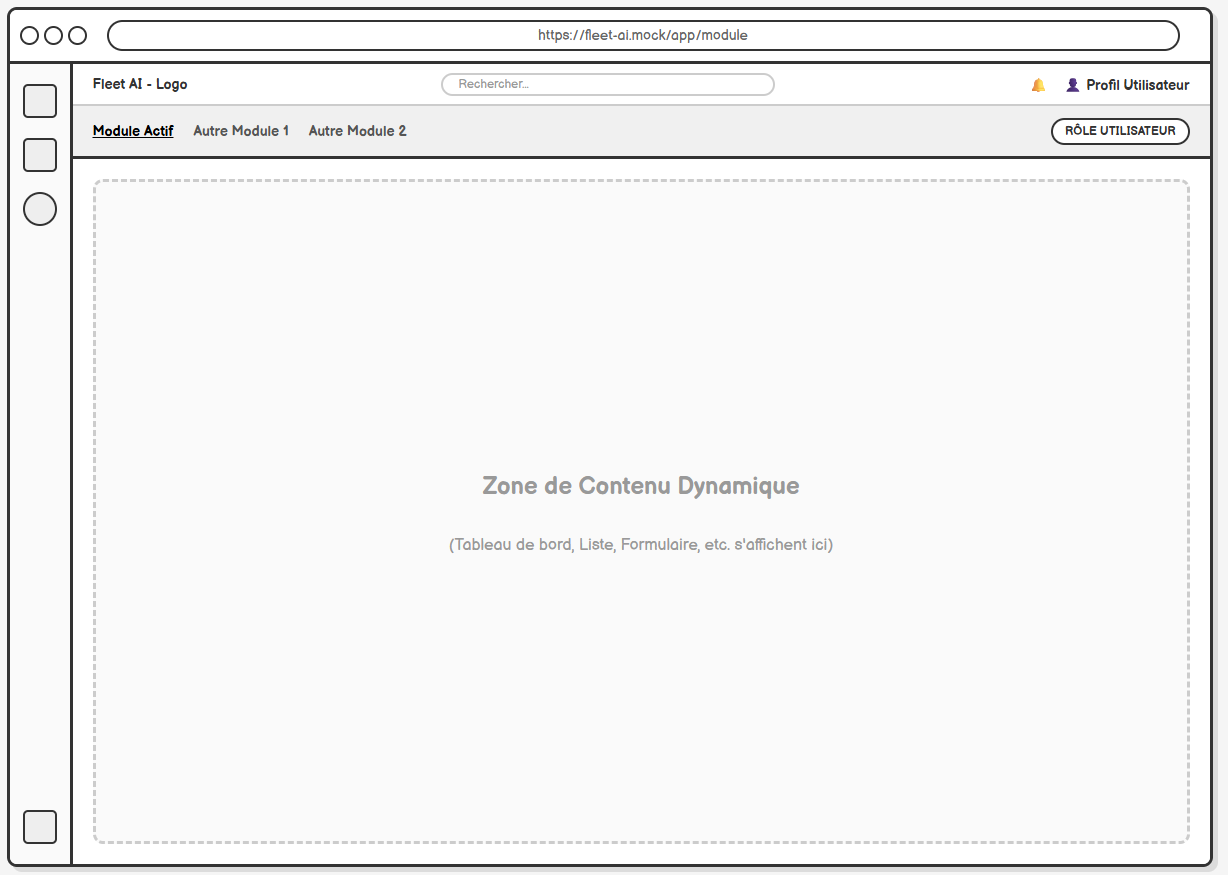
\includegraphics[width=0.9\linewidth, height=0.36\textheight, keepaspectratio]{img/maquette/maquette_layout_commun}
\caption{Maquette du layout commun de l'application}
\label{fig:maquette-layout-commun}
\end{figure}

\begin{figure}[H]
\centering
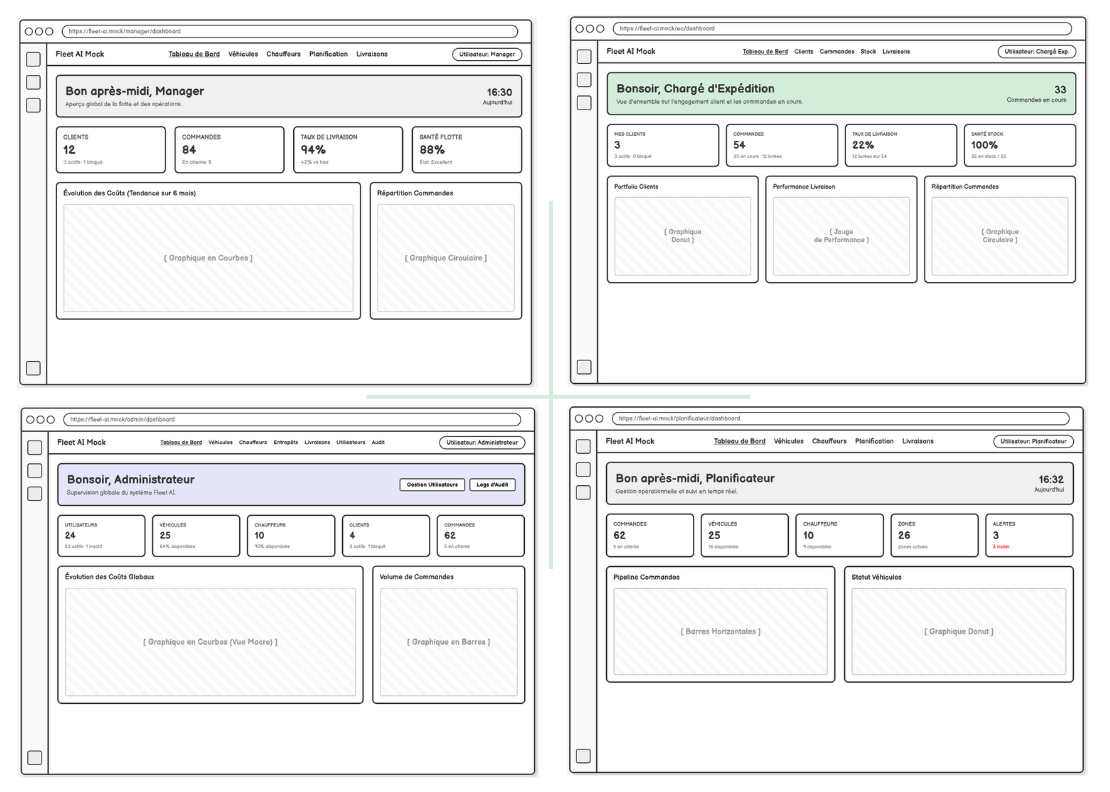
\includegraphics[width=0.9\linewidth, height=0.36\textheight, keepaspectratio]{img/maquette/maquette_dashboards}
\caption{Maquette de l'interface du tableau de bord}
\label{fig:maquette-dashboard}
\end{figure}

\begin{figure}[H]
\centering
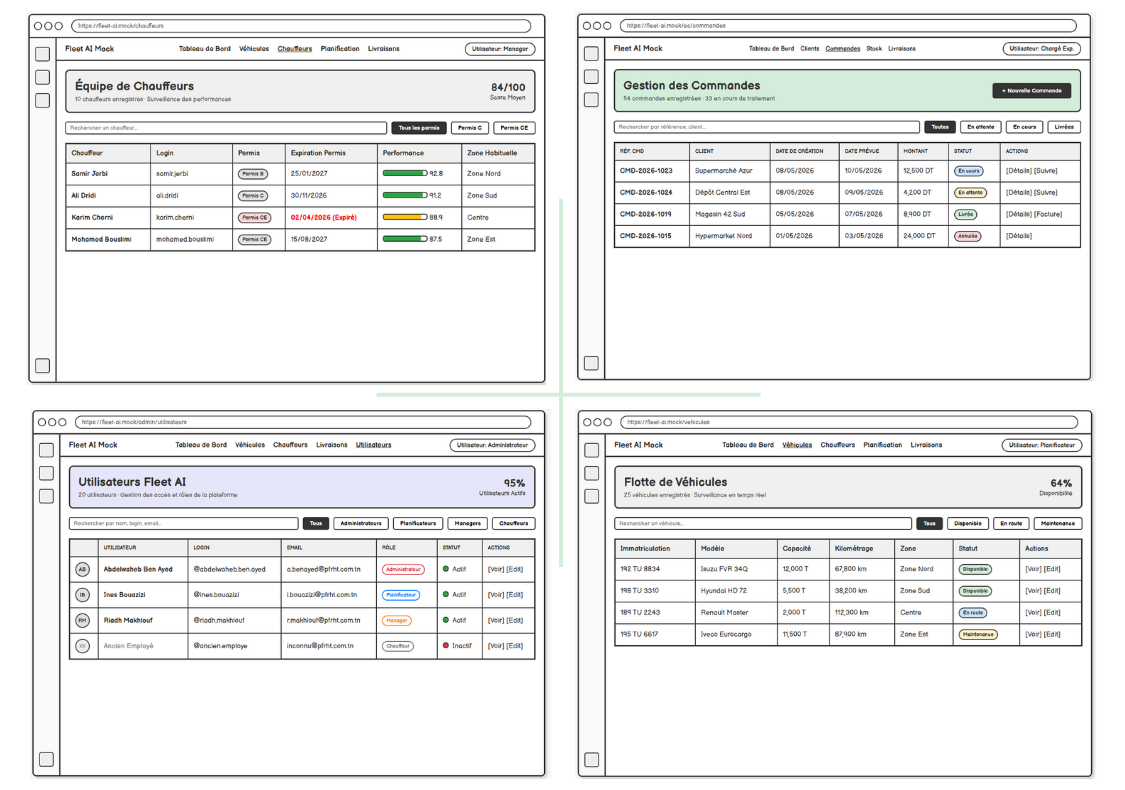
\includegraphics[width=0.9\linewidth, height=0.36\textheight, keepaspectratio]{img/maquette/maquette_desListes}
\caption{Maquette des interfaces de listes de données}
\label{fig:maquette-listes}
\end{figure}

\begin{figure}[H]
\centering
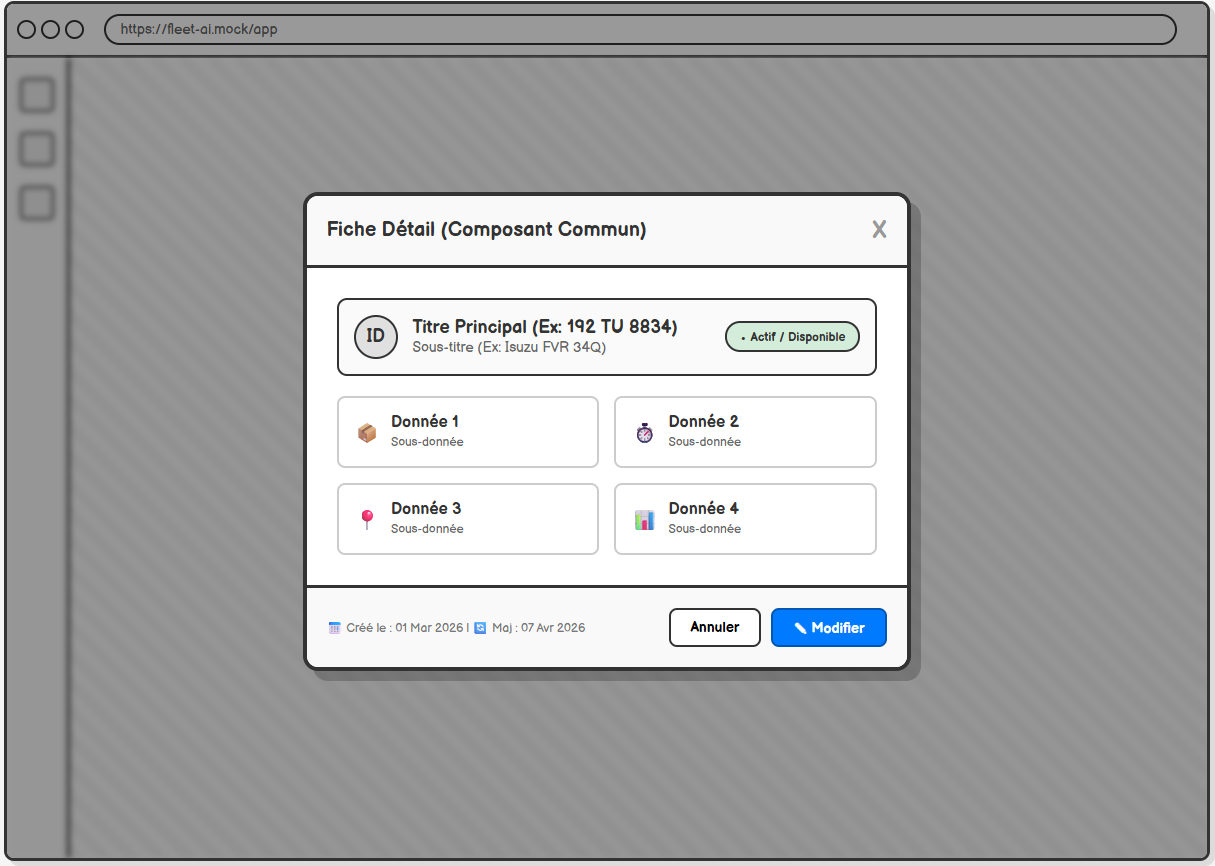
\includegraphics[width=0.9\linewidth, height=0.36\textheight, keepaspectratio]{img/maquette/maquette_modifier}
\caption{Maquette de l'interface de modification d'entité}
\label{fig:maquette-modifier}
\end{figure}

\begin{figure}[H]
\centering
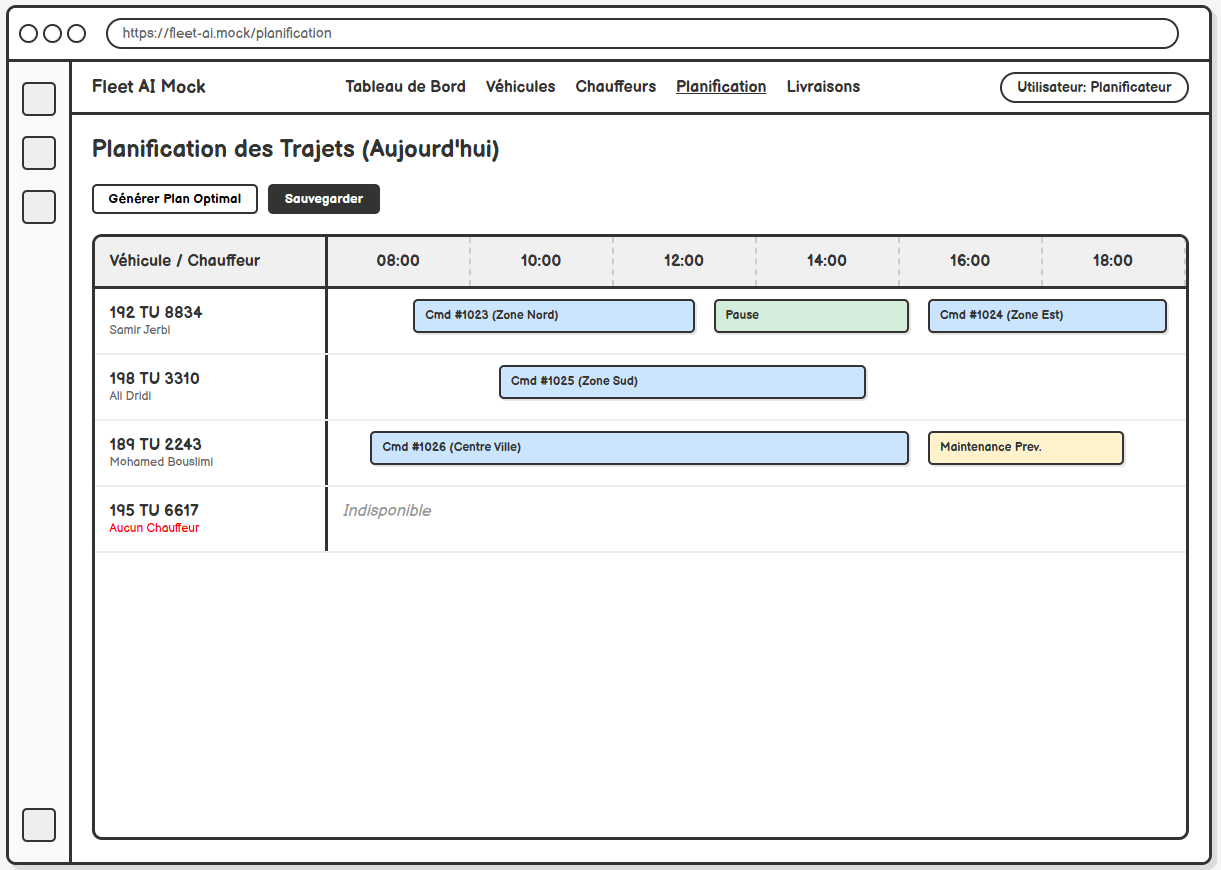
\includegraphics[width=0.9\linewidth, height=0.36\textheight, keepaspectratio]{img/maquette/maquette_disponibilite_desChauffeurs}
\caption{Maquette de l'interface de disponibilité des chauffeurs}
\label{fig:maquette-chauffeurs}
\end{figure}

\begin{figure}[H]
\centering
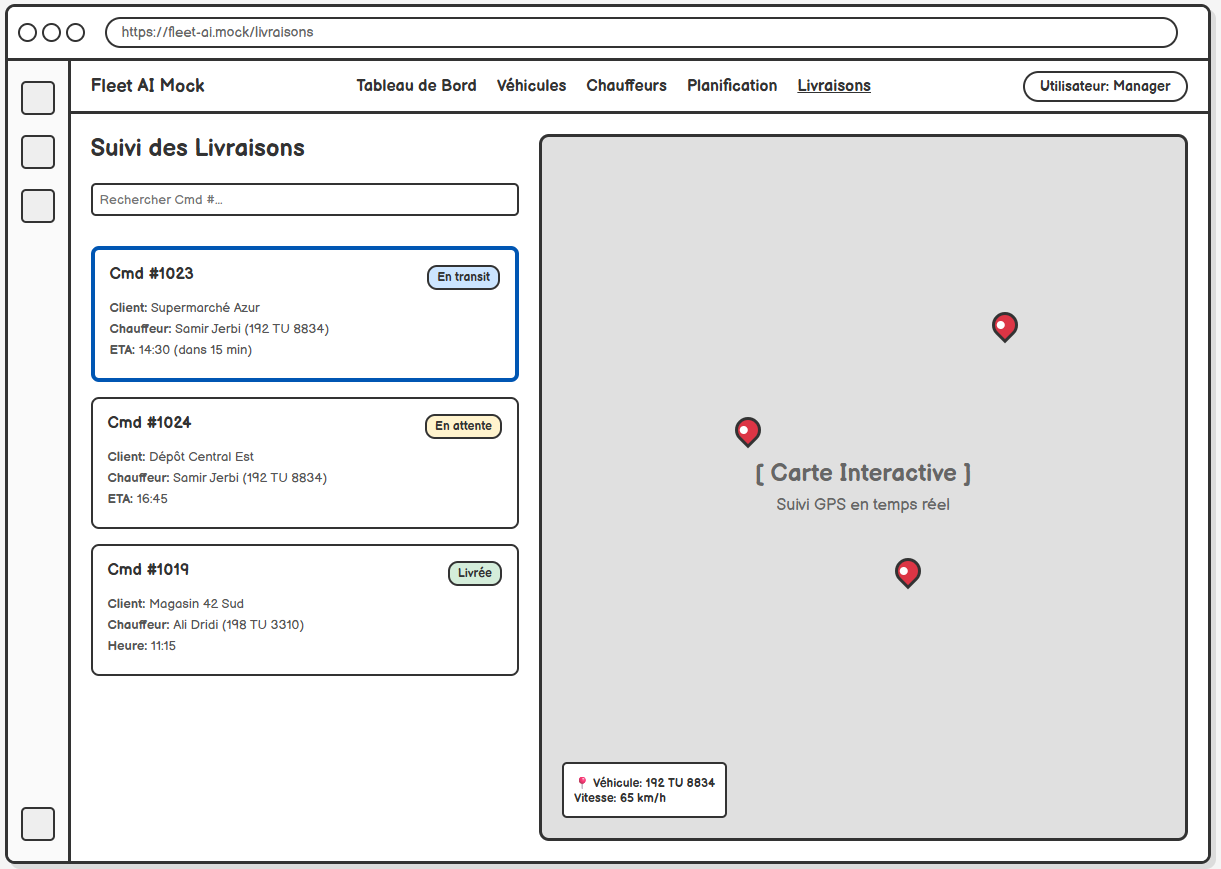
\includegraphics[width=0.9\linewidth, height=0.36\textheight, keepaspectratio]{img/maquette/maquette_suivi_livraison_endirect}
\caption{Maquette de la page de suivi des livraisons en direct}
\label{fig:maquette-planification}
\end{figure}

\subsection{Technologies à utiliser}

Le tableau ci-dessous liste les technologies retenues pour Fleet~AI.

\setlength{\arrayrulewidth}{1pt}
\begin{longtable}{|>{\raggedright\arraybackslash}p{4cm}|>{\raggedright\arraybackslash}p{3.5cm}|>{\raggedright\arraybackslash}p{7.5cm}|}
\hline
\rowcolor{headerbg}
\textbf{Technologie} & \textbf{Domaine} & \textbf{Rôle dans le projet} \\
\hline
\endfirsthead
\hline
\rowcolor{headerbg}
\textbf{Technologie} & \textbf{Domaine} & \textbf{Rôle dans le projet} \\
\hline
\endhead
\hline
\endfoot

Angular 19 + PrimeNG & Interface web & Application web Fleet~AI intégrée à la plateforme WFMS existante. \\
\hline
Flutter / Dart & Application mobile & Application mobile chauffeur et client (Android et iOS). \\
\hline
Spring Boot 3.4 & Backend & Services métier, API REST, sécurité et persistance des données. \\
\hline
Python / Flask & Passerelle & Passerelle WFMS existante gérant l'authentification centralisée. \\
\hline
Python / FastAPI & Service IA & Microservice dédié à l'optimisation des itinéraires et à la prédiction. \\
\hline
PostgreSQL & Base de données & Données structurées (utilisateurs, véhicules, commandes, paiements). \\
\hline
MongoDB & Base de données & Journaux d'audit applicatifs. \\
\hline
Redis & Cache & Mise en cache des données fréquemment consultées (KPIs, ressources). \\
\hline

\caption{Technologies retenues pour le projet Fleet~AI}
\end{longtable}
\setlength{\arrayrulewidth}{0.4pt}

\subsection{Contrainte technique : intégration WFMS et ERP}

Fleet~AI est une \textbf{application additionnelle} qui s'exécute dans un écosystème technique existant et en production. Cette contrainte impose deux règles architecturales non négociables.

\textbf{Intégration avec WFMS :}
\begin{itemize}[leftmargin=2.5em]
    \item[$\bullet$] Toutes les requêtes vers Fleet~AI transitent par la \textbf{passerelle Flask} de WFMS, qui gère l'authentification, le déchiffrement des tokens RSA et le routage.
    \item[$\bullet$] Le RBAC de Fleet~AI est aligné sur le système de rôles WFMS : AD, PL, MG, CH, REC, CL.
    \item[$\bullet$] L'interface Angular de Fleet~AI est intégrée dans la navigation latérale WFMS, avec le même thème PrimeNG et les mêmes mécanismes de session.
\end{itemize}

\textbf{Intégration avec l'ERP Poulina :}
\begin{itemize}[leftmargin=2.5em]
    \item[$\bullet$] Fleet~AI lit le stock réel depuis l'ERP via un adaptateur ETL en quasi temps réel.
    \item[$\bullet$] Quand une commande est acceptée dans Fleet~AI, elle est transmise à l'ERP pour préparation. L'ERP retourne le statut \textit{Prête} quand la commande est disponible pour l'affectation.
    \item[$\bullet$] Fleet~AI ne modifie pas le fonctionnement interne de l'ERP.
\end{itemize}

\subsection{Durée du projet}

Le projet a été réalisé sur une période de 4 mois (Février -- Mai 2025), organisée en cinq sprints de deux semaines.

\subsection{Livrables du projet}

À l'issue de ces travaux de conception et de développement, les livrables finaux fournis à GREPSYS et PGH sont structurés comme suit :
\begin{itemize}[leftmargin=2.5em]
    \item[$\bullet$] \textbf{Le code source complet :} L'ensemble du code backend (Spring Boot, FastAPI) et frontend (Angular).
    \item[$\bullet$] \textbf{L'application web :} Interface d'administration et de gestion déployée et intégrée au WFMS.
    \item[$\bullet$] \textbf{L'application mobile :} L'application Flutter (Android/iOS) destinée aux chauffeurs et aux clients.
    \item[$\bullet$] \textbf{Les modèles IA :} Les modèles de Machine Learning entraînés pour la prédiction et l'assistant conversationnel.
    \item[$\bullet$] \textbf{La documentation technique :} Les manuels d'architecture, de déploiement et d'utilisation de la plateforme.
    \item[$\bullet$] \textbf{La présentation du projet :} Support de présentation destiné à l'équipe logistique de PGH pour l'adoption du système.
\end{itemize}

\section*{Conclusion}
\addcontentsline{toc}{section}{Conclusion}
Ce chapitre a présenté GREPSYS Tunisia, Poulina Group Holding et le cahier des charges complet de Fleet~AI, incluant les fonctionnalités, les maquettes, les contraintes d'intégration WFMS/ERP et les livrables du projet. Le chapitre suivant analyse les solutions de gestion de flotte disponibles sur le marché et explique pourquoi aucune ne répond au besoin de PGH.


% ---- Chapitre 2 : Étude préalable ----
\chapter{Etude préalable}

\minitocsection

\section*{Introduction}
\addcontentsline{toc}{section}{Introduction}
Ce chapitre présente l'état actuel de la gestion logistique chez Poulina Group Holding, dresse un état de l'art des principales applications commerciales de gestion de flotte et en identifie les limites vis-à-vis des contraintes spécifiques de PGH. Il expose enfin les raisons pour lesquelles le développement sur mesure de Fleet~AI s'impose comme la seule solution viable.

% =============================================================
\section{Etude de l'existant}
% =============================================================

\subsection{Description des procédures actuelles}

Chez Poulina Group Holding, la gestion logistique repose intégralement sur des procédés manuels : un seul planificateur répartit les missions par téléphone, sans système centralisé. Les principales limites observées sont :

\begin{itemize}
  \item Aucune visibilité sur les commandes en attente ni priorisation objective.
  \item Itinéraires construits empiriquement, sans optimisation ni suivi GPS.
  \item Preuves de livraison informelles : pas de signature numérique, pas de photo horodatée.
  \item Encaissements non rapprochés automatiquement avec les commandes correspondantes.
  \item Absence de données opérationnelles exploitables : tout incident disparaît sans être tracé.
\end{itemize}

\subsection{Etude comparative des solutions existantes}

La gestion de flotte est un domaine couvert par plusieurs plateformes commerciales. Pour identifier les meilleures pratiques et évaluer leur adéquation aux besoins de PGH, nous avons étudié trois applications majeures : \textbf{Geotab}, \textbf{Samsara} et \textbf{Verizon Connect}.

\subsubsection*{Geotab}
Geotab est une plateforme très orientée télématique véhiculaire. Elle propose un suivi GPS avancé, des rapports de conduite détaillés et une intégration avec de nombreux partenaires via une marketplace ouverte. Sa forte dépendance aux boîtiers OBD physiques complique cependant le déploiement rapide sur une flotte hétérogène, et son interface nécessite une formation approfondie.

\begin{figure}[H]
\centering
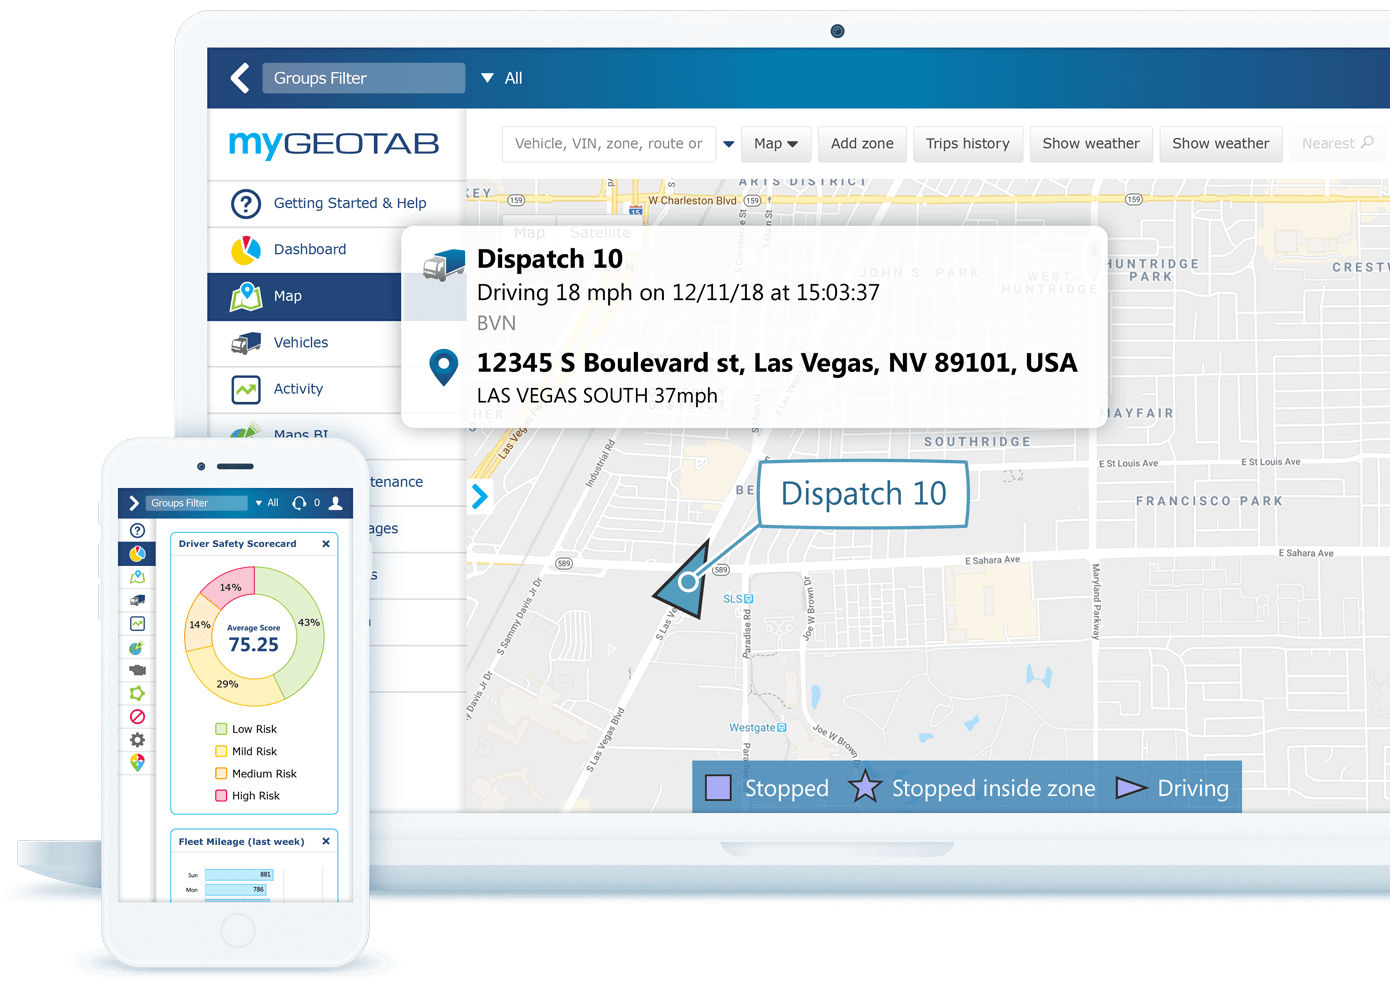
\includegraphics[width=0.85\linewidth]{img/geotab_screenshot}
\caption{Interface de la plateforme Geotab --- tableau de bord de suivi de flotte}
\label{fig:geotab-screenshot}
\end{figure}

\subsubsection*{Samsara}
Samsara est considérée comme l'une des plateformes les plus complètes du marché. Elle se distingue par l'intégration de caméras IA embarquées, un suivi GPS performant et des outils analytiques avancés. Néanmoins, la dépendance matérielle (caméras IA embarquées) constitue un frein logistique majeur pour un déploiement en Tunisie.

\begin{figure}[H]
\centering
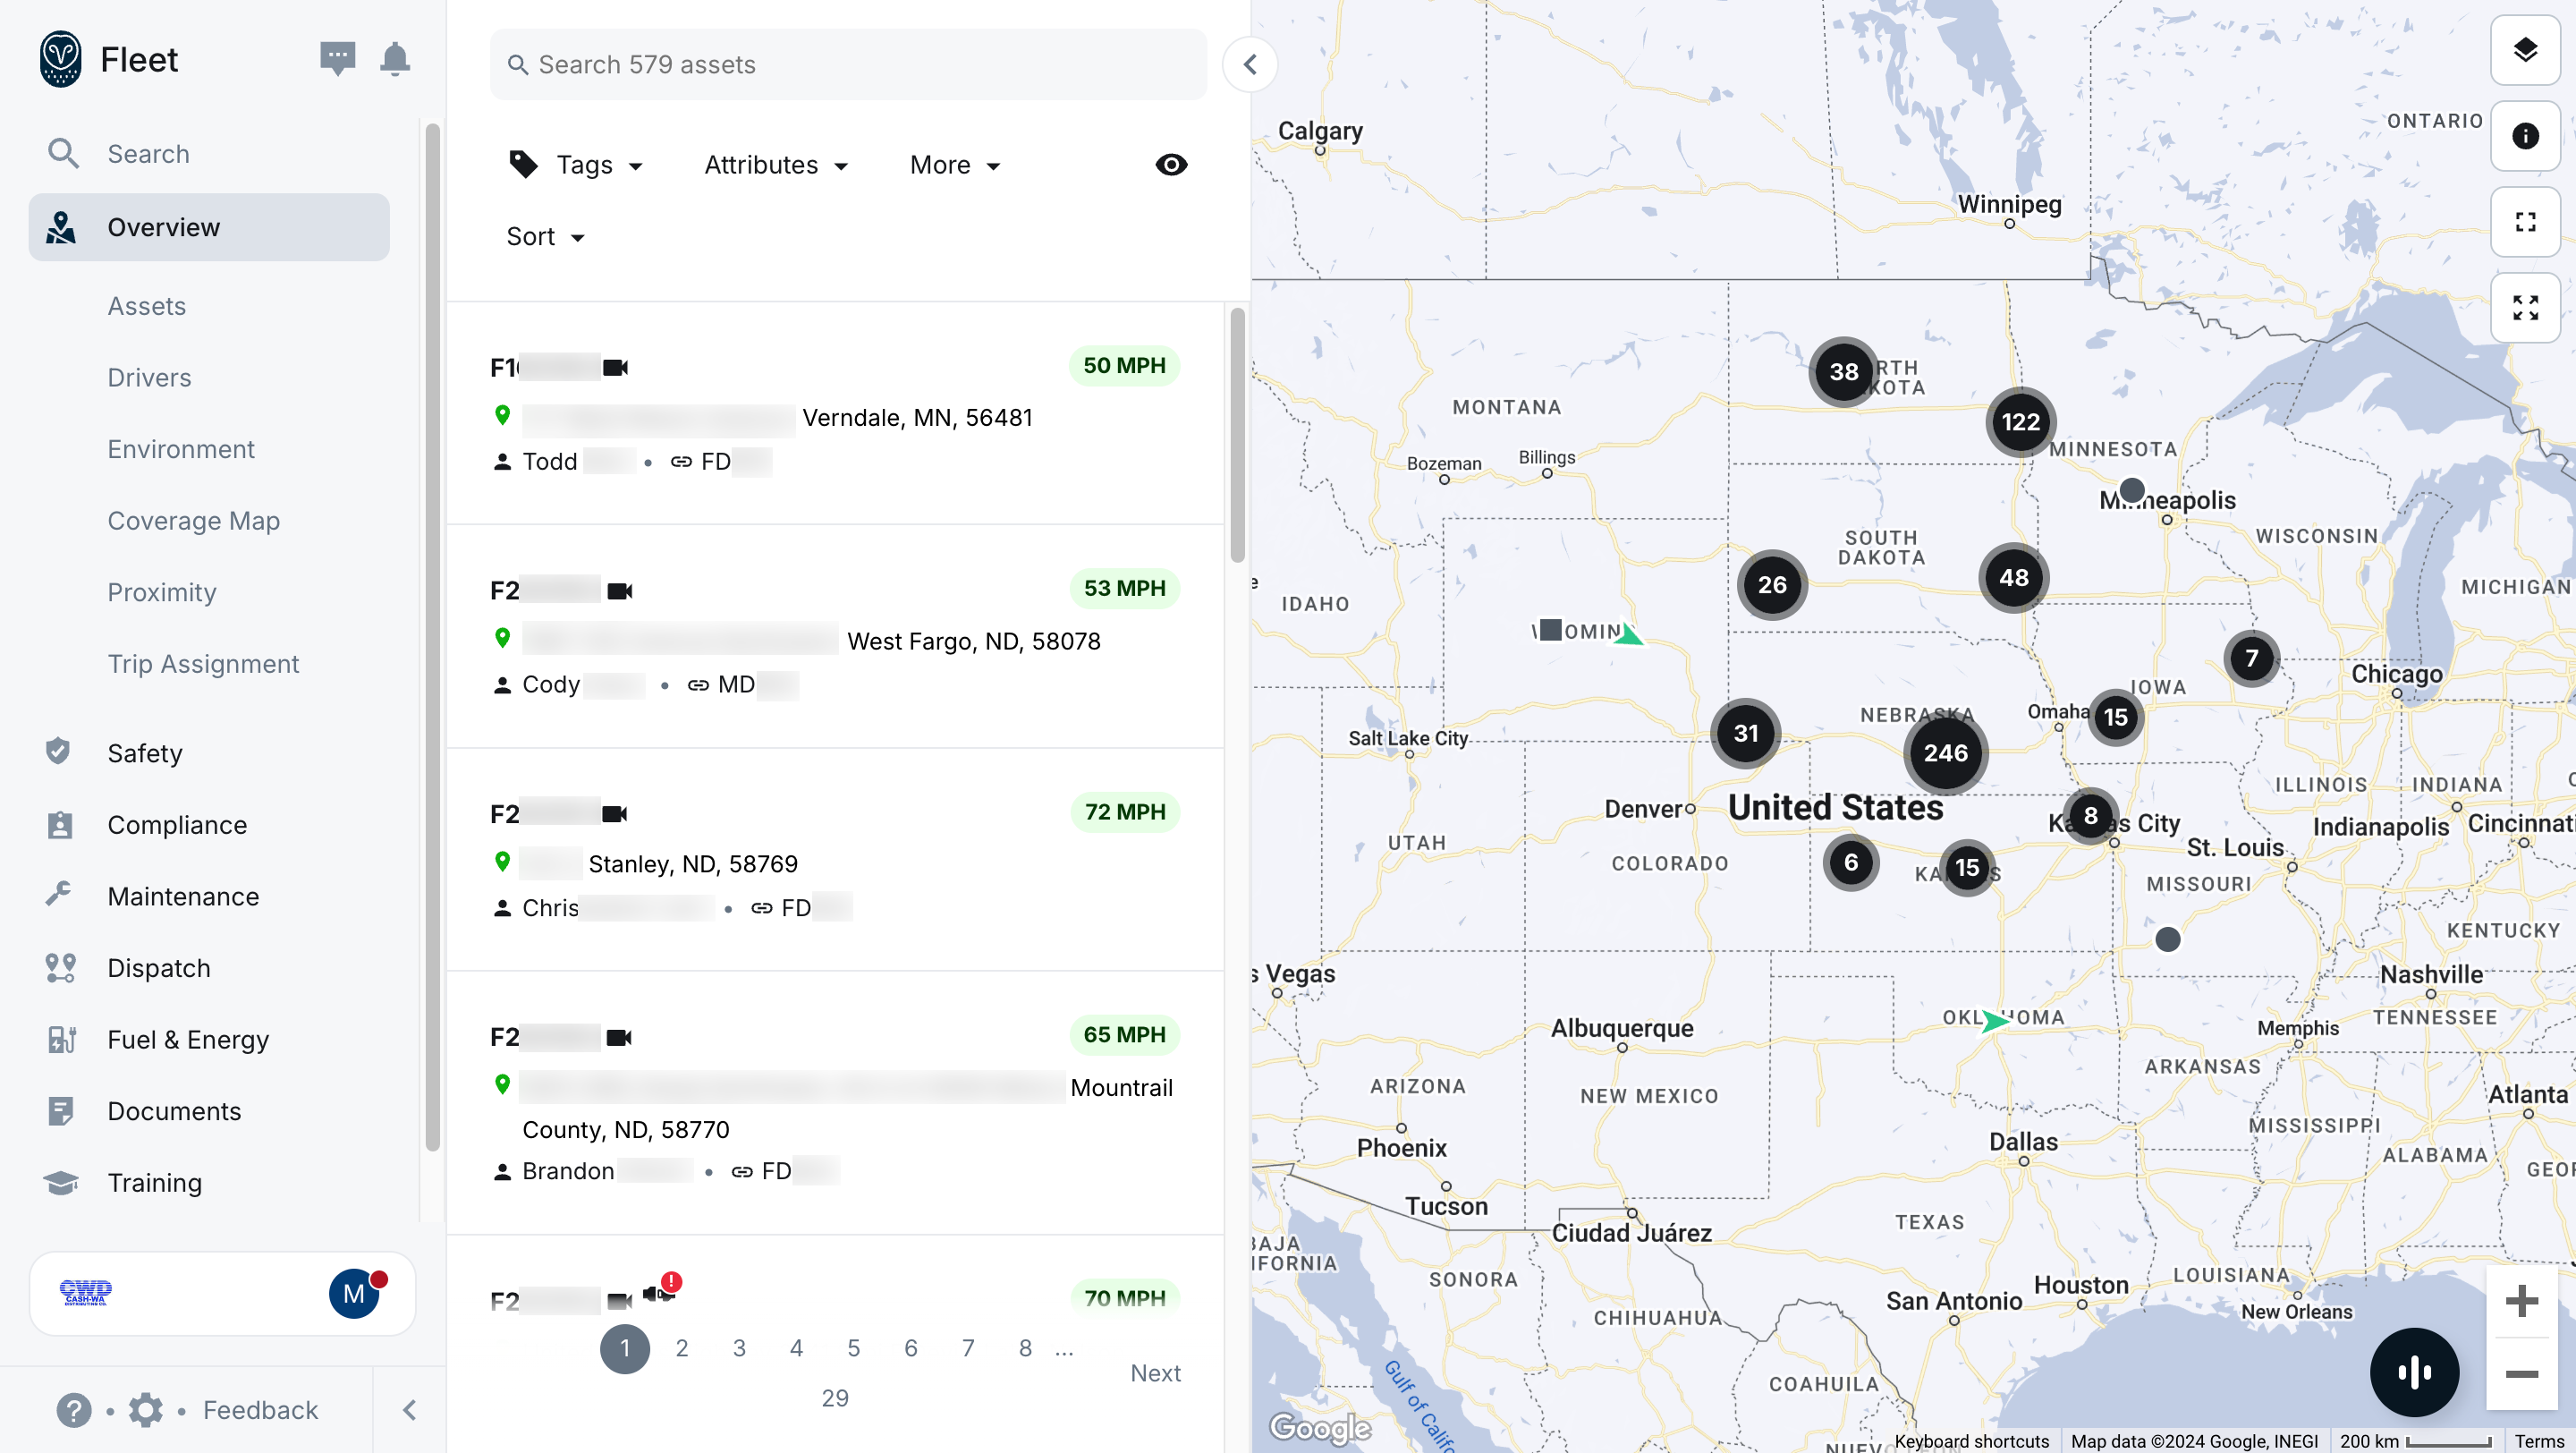
\includegraphics[width=0.85\linewidth]{img/samsara_screenshot}
\caption{Interface de la plateforme Samsara --- tableau de bord analytique}
\label{fig:samsara-screenshot}
\end{figure}

\subsubsection*{Verizon Connect}
Verizon Connect intègre un suivi GPS standard, la gestion des conducteurs et des alertes automatiques. Ses fonctionnalités analytiques manquent cependant de profondeur, et son API s'avère trop limitée pour une intégration poussée avec des systèmes d'information tiers.

\begin{figure}[H]
\centering
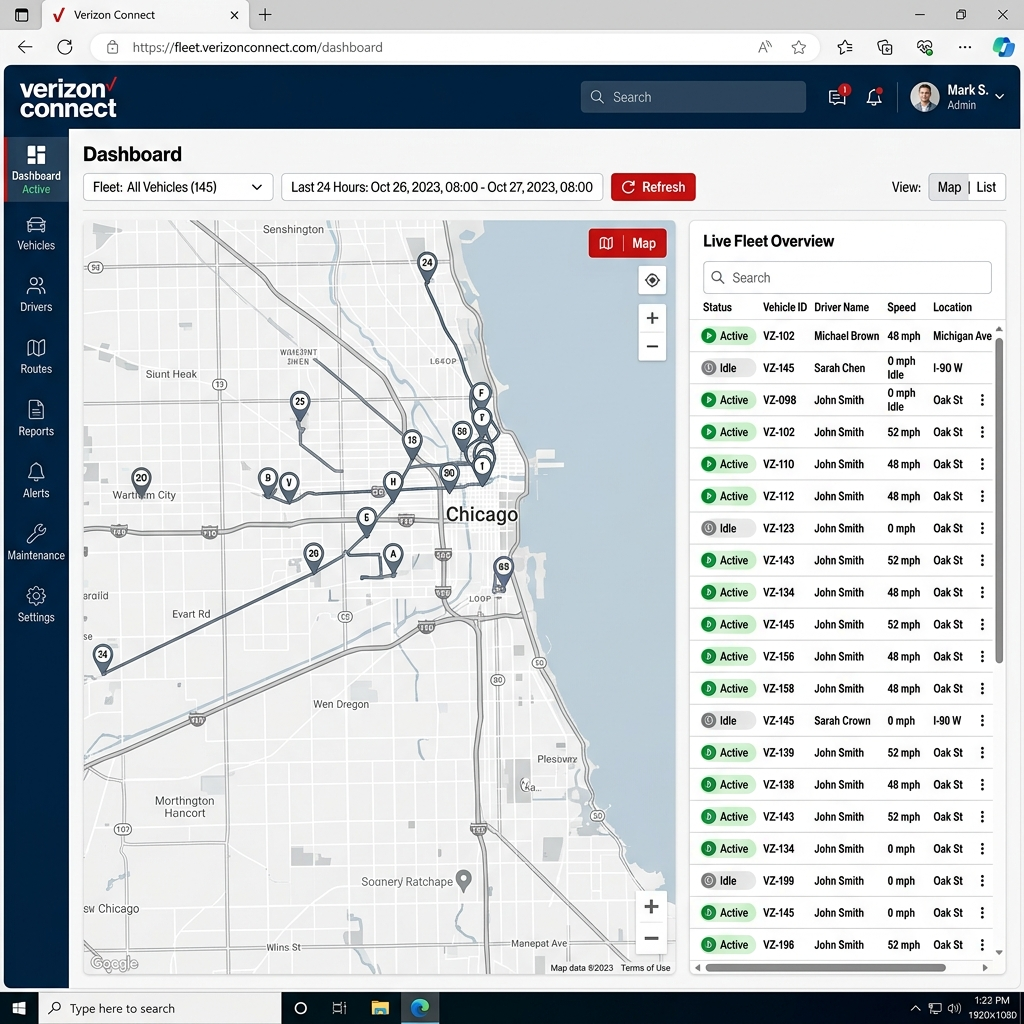
\includegraphics[width=0.85\linewidth]{img/verizon_screenshot}
\caption{Interface de la plateforme Verizon Connect --- vue de suivi des véhicules}
\label{fig:verizon-screenshot}
\end{figure}

\subsubsection*{Comparaison des fonctionnalités}
Le tableau ci-dessous synthétise les fonctionnalités offertes par ces trois applications.

\setlength{\arrayrulewidth}{1pt}
\begin{longtable}{|>{\raggedright\arraybackslash}p{3.5cm}|>{\raggedright\arraybackslash}p{3.5cm}|>{\raggedright\arraybackslash}p{3.5cm}|>{\raggedright\arraybackslash}p{3.5cm}|}
  \hline
  \rowcolor{headerbg}
  \textbf{Fonctionnalité} & \textbf{Geotab} & \textbf{Samsara} & \textbf{Verizon Connect} \\
  \hline
  \endfirsthead

  \hline
  \rowcolor{headerbg}
  \textbf{Fonctionnalité} & \textbf{Geotab} & \textbf{Samsara} & \textbf{Verizon Connect} \\
  \hline
  \endhead

  Suivi GPS temps réel & Oui, très avancé & Oui, intégré & Oui \\
  \hline
  Gestion des chauffeurs & Basique & Avancée (caméra IA) & Basique \\
  \hline
  Gestion des véhicules & Complète & Complète & Complète \\
  \hline
  Zones géographiques & Oui (géofencing) & Oui (géofencing) & Oui (géofencing) \\
  \hline
  Tableau de bord & Personnalisable & Moderne et intuitif & Standard \\
  \hline
  Gestion des coûts & Via marketplace & Intégrée & Basique \\
  \hline
  Contrôle d'accès (RBAC) & Limité & Basique & Limité \\
  \hline
  Intégration ERP/SI & API ouverte & API ouverte & API limitée \\
  \hline
  Audit/Traçabilité & Limité & Partiel & Limité \\
  \hline
  Hébergement & Cloud uniquement & Cloud uniquement & Cloud uniquement \\
  \hline
\caption{Comparaison des applications de gestion de flotte existantes}
\end{longtable}
\setlength{\arrayrulewidth}{0.4pt}

% =============================================================
\section{Critique de l'existant}
% =============================================================

L'analyse du fonctionnement actuel chez PGH et l'étude des solutions commerciales disponibles font apparaître des lacunes structurelles qui justifient pleinement le développement d'une solution sur mesure.

\subsubsection*{Limites organisationnelles du système actuel :}
\begin{itemize}
  \item La concentration de la planification sur un seul acteur crée un point de défaillance unique et limite la capacité de traitement lors des pics d'activité.
  \item La communication orale entre planificateur et chauffeurs génère des pertes d'information et une absence totale de traçabilité des échanges.
  \item L'absence d'optimisation des itinéraires entraîne une consommation excessive de carburant et un non-respect fréquent des créneaux horaires contractuels.
  \item Sans suivi GPS ni preuve de livraison numérique, il est impossible de détecter les retards, de résoudre les litiges ou de garantir la conformité des remises de marchandises.
  \item L'informalité des encaissements expose l'entreprise à des risques financiers et à des écarts comptables non détectés.
\end{itemize}

\subsubsection*{Incompatibilités des solutions commerciales étudiées :}
\begin{itemize}
  \item[$\bullet$] \textbf{Hébergement cloud exclusif :} Ces applications fonctionnent uniquement en mode SaaS, ce qui pose des problèmes critiques de souveraineté des données pour PGH, qui exige un déploiement on-premise.
  \item[$\bullet$] \textbf{Coût prohibitif :} Les tarifications par abonnement mensuel et par véhicule sont inadaptées à l'échelle de la flotte de PGH.
  \item[$\bullet$] \textbf{Absence d'intégration WFMS :} Aucune solution ne propose d'intégration native avec la plateforme WFMS du groupe ; des développements middleware coûteux seraient nécessaires.
  \item[$\bullet$] \textbf{Contrôle d'accès inadapté :} Les systèmes de permissions ne correspondent pas à la hiérarchie spécifique requise par PGH (Administrateur, Planificateur, Manager, Chauffeur, Responsable Engagement Client -- REC, Client).
  \item[$\bullet$] \textbf{Disponibilité locale limitée :} Le support technique en Tunisie de ces éditeurs internationaux est insuffisant pour garantir une continuité de service critique.
\end{itemize}

Ces constats démontrent qu'aucune solution du marché ne peut répondre simultanément aux exigences de déploiement on-premise, d'intégration WFMS, de contrôle d'accès hiérarchique et de couverture fonctionnelle métier propres à PGH. Le développement sur mesure de Fleet~AI s'impose donc comme la seule approche viable.

% =============================================================
\section{Solution proposée}
% =============================================================

Face à ces limites, PGH a fait le choix stratégique du développement sur mesure avec la création de \textbf{Fleet~AI} par GREPSYS. Cette solution est déployée directement sur les serveurs de PGH (on-premise) et s'intègre nativement à la plateforme WFMS existante, sans en modifier le code source.

Fleet~AI couvre l'ensemble du cycle logistique à travers cinq modules principaux :

\begin{itemize}
  \item La planification assistée avec optimisation algorithmique des itinéraires et affectation guidée.
  \item Une application mobile pour les chauffeurs garantissant la collecte de preuves de livraison numériques et supportant un mode hors-ligne.
  \item L'intégration de modèles d'intelligence artificielle pour prédire la demande par zone et anticiper les retards de livraison.
  \item La mise en place de tableaux de bord décisionnels et de KPIs centralisés à l'échelle du holding.
  \item La gestion numérisée des paiements et des réclamations avec traçabilité complète de chaque opération terrain.
\end{itemize}

\section*{Conclusion}
\addcontentsline{toc}{section}{Conclusion}
L'étude de l'existant a mis en évidence qu'aucune plateforme du marché, telles que Geotab, Samsara ou Verizon Connect, ne pouvait répondre aux exigences de PGH. Leurs limites en matière de coût, de déploiement cloud (SaaS), d'intégration au WFMS et de gestion des rôles les rendent inadaptées. C'est pourquoi le développement sur mesure de Fleet~AI s'est imposé comme la seule approche viable. Le chapitre suivant détaille la méthodologie et l'architecture adoptées pour concrétiser cette solution.


% ---- Chapitre 3 : Méthodologie et environnement ----
\chapter{Méthodologie et environnement de travail}

\section*{Introduction}
\addcontentsline{toc}{section}{Introduction}
Ce chapitre décrit les choix méthodologiques et techniques du projet : pourquoi Scrum, comment le Product Backlog est structuré, quels outils et quelle architecture ont été retenus.

% =============================================================
\section{Choix de la méthode de gestion de projet}
% =============================================================

\subsection{Les méthodes de gestion de projet}
Deux grandes familles de méthodes s'offrent pour la gestion d'un tel projet : Agile et Traditionnelle.

\definecolor{headerbg}{HTML}{d5f5e3}
\setlength{\arrayrulewidth}{1pt}
\begin{longtable}{|>{\raggedright\arraybackslash}p{3cm}|>{\raggedright\arraybackslash}p{5.5cm}|>{\raggedright\arraybackslash}p{6.5cm}|}
\hline
\rowcolor{headerbg}
\textbf{Méthode} & \textbf{Avantages} & \textbf{Inconvénients} \\
\hline
\endfirsthead
\endfoot

\textbf{Agile}
&
\begin{itemize}[left=0pt, topsep=0pt, itemsep=0pt, parsep=0pt, partopsep=0pt]
    \item[$\bullet$] Flexibilité
    \item[$\bullet$] Livraisons fréquentes
    \item[$\bullet$] Collaboration renforcée
    \item[$\bullet$] Amélioration continue
    \item[$\bullet$] Réduction des risques
\end{itemize}
&
\begin{itemize}[left=0pt, topsep=0pt, itemsep=0pt, parsep=0pt, partopsep=0pt]
    \item[$\bullet$] Moins de prévisibilité
    \item[$\bullet$] Documentation limitée
    \item[$\bullet$] Dépendance à l'implication du client
    \item[$\bullet$] Risque de dérive du périmètre
\end{itemize}
\\
\hline

\textbf{Traditionnelle}
&
\begin{itemize}[left=0pt, topsep=0pt, itemsep=0pt, parsep=0pt, partopsep=0pt]
    \item[$\bullet$] Planification détaillée
    \item[$\bullet$] Budget et délais définis
    \item[$\bullet$] Documentation exhaustive
    \item[$\bullet$] Structure hiérarchique claire
\end{itemize}
&
\begin{itemize}[left=0pt, topsep=0pt, itemsep=0pt, parsep=0pt, partopsep=0pt]
    \item[$\bullet$] Rigidité
    \item[$\bullet$] Livraison tardive
    \item[$\bullet$] Moins d'implication du client
    \item[$\bullet$] Risque d'effet tunnel
\end{itemize}
\\
\hline

\caption{Comparaison entre méthode traditionnelle et méthode Agile}
\end{longtable}
\setlength{\arrayrulewidth}{0.4pt}

\subsection*{Pourquoi Scrum ?}
Nous avons choisi Scrum car :
\begin{itemize}
    \item[$\bullet$] Les besoins de PGH ont évolué en cours de projet (règles de paiement, validation des livraisons), rendant toute planification rigide inadaptée.
    \item[$\bullet$] Le système est multi-composants (web Angular, mobile Flutter, back-end Spring Boot, IA FastAPI) avec des dépendances fortes entre modules.
    \item[$\bullet$] Les 4 mois de développement imposaient des livraisons fréquentes et validées à chaque itération par GREPSYS et PGH.
\end{itemize}

% =============================================================
\subsection{Méthodologie SCRUM}
% =============================================================

Le développement s'est organisé autour du cycle de vie Scrum, rythmé par des sprints de deux semaines produisant à chaque itération un incrément fonctionnel livrable. \cite{scrum_guide}

\begin{figure}[H]
\centering
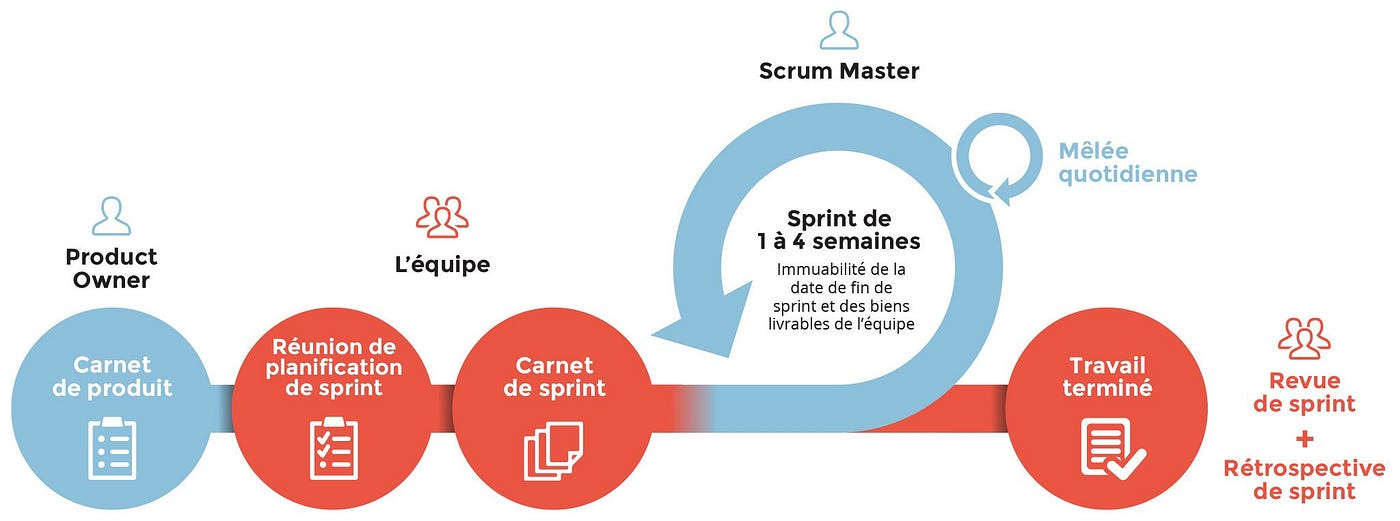
\includegraphics[width=0.65\linewidth]{img/logo/logo_scrum}
\caption{Le cycle de vie Scrum}
\label{fig:scrum-cycle}
\end{figure}

\paragraph*{Rôles Scrum}

\setlength{\arrayrulewidth}{1pt}
\begin{table}[H]
\centering
\begin{tabular}{|p{4cm}|p{11cm}|}
\hline
\rowcolor{headerbg}
\textbf{Rôle} & \textbf{Personne(s)} \\
\hline
Product Owner & M. Marouen Bouallegui \\
\hline
Scrum Master & Mme Lamia Mansouri\\
\hline
Équipe de développement & Mohamed Malek Ben Jemaa et Islem Gharsallah \\
\hline
\end{tabular}
\caption{Répartition des rôles Scrum}
\end{table}
\setlength{\arrayrulewidth}{0.4pt}

% =============================================================
\subsection{Product Backlog}
% =============================================================

Le Product Backlog suivant présente l'ensemble des user stories du projet, organisées en cinq sprints thématiques et priorisées sur une échelle de 1 à 3 (1 étant la priorité maximale).

\definecolor{headerbg}{HTML}{d5f5e3}
\definecolor{sprints}{HTML}{b8e6c8}
\renewcommand{\arraystretch}{0.88}
\setlength{\arrayrulewidth}{1pt}
\begin{longtable}{|c|>{\raggedright\arraybackslash}p{13cm}|c|}
\hline

\rowcolor{headerbg}
\textbf{ID} & \textbf{User Story} & \textbf{Priorité} \\
\hline
\endfirsthead

\rowcolor{headerbg}
\textbf{ID} & \textbf{User Story (suite)} & \textbf{Priorité} \\
\hline
\endhead

\multicolumn{3}{|>{\columncolor{sprints}}c|}{\textbf{Sprint 1 --- Fondation \& Gestion des Ressources} (S1--S2 $\mid$ 25 US)} \\\hline

US-001 & En tant qu'utilisateur, je veux me connecter avec mes identifiants habituels afin d'accéder aux fonctionnalités Fleet~AI correspondant à mon rôle. & 1 \\\hline
US-002 & En tant qu'Administrateur, je veux que les droits de chaque utilisateur soient contrôlés à chaque accès afin que chacun n'utilise que les fonctionnalités autorisées par son rôle. & 1 \\\hline
US-003 & En tant qu'Administrateur, je veux gérer les comptes utilisateurs afin de contrôler les accès au système. & 1 \\\hline
US-004 & En tant qu'Administrateur, je veux assigner un rôle à chaque utilisateur afin de définir ses permissions. & 1 \\\hline
US-005 & En tant qu'Administrateur, je veux gérer les zones géographiques de livraison afin de structurer les opérations par région. & 1 \\\hline
US-006 & En tant qu'Administrateur, je veux consulter le journal d'audit du système afin de tracer toutes les actions critiques. & 1 \\\hline
US-007 & En tant qu'Administrateur, je veux déclencher des sauvegardes des données afin de protéger les informations du système. & 2 \\\hline
US-008 & En tant qu'Administrateur, je veux consulter le tableau de bord avec les statistiques générales afin de superviser l'état du système. & 1 \\\hline
US-009 & En tant que Planificateur, je veux consulter la liste des véhicules avec leur statut afin de connaître les ressources disponibles. & 1 \\\hline
US-010 & En tant qu'Administrateur, je veux gérer les véhicules afin de maintenir le référentiel à jour. & 1 \\\hline
US-011 & En tant que Planificateur, je veux marquer un véhicule en maintenance afin de le retirer temporairement de la planification. & 2 \\\hline
US-012 & En tant que Manager, je veux consulter le taux d'utilisation des véhicules afin d'optimiser la flotte. & 2 \\\hline
US-013 & En tant que Manager, je veux consulter les coûts par véhicule afin de suivre les dépenses opérationnelles. & 2 \\\hline
US-014 & En tant que Planificateur, je veux consulter la disponibilité des chauffeurs afin de planifier les affectations. & 1 \\\hline
US-015 & En tant que Planificateur, je veux consulter les performances des chauffeurs afin de guider les affectations. & 2 \\\hline
US-016 & En tant que Manager, je veux consulter le classement des chauffeurs afin d'identifier les plus et les moins performants. & 2 \\\hline
US-017 & En tant qu'Administrateur, je veux configurer les indicateurs de performance des chauffeurs afin d'adapter le calcul du score global. & 2 \\\hline
US-018 & En tant que Chauffeur, je veux me connecter à l'application mobile afin d'accéder à mes fonctionnalités Fleet~AI. & 1 \\\hline
US-019 & En tant que Chauffeur, je veux consulter mes indicateurs de performance depuis l'application mobile afin de suivre mon activité. & 2 \\\hline
US-020 & En tant que Chauffeur, je veux déclarer ma disponibilité depuis l'application mobile afin de signaler mes périodes de présence. & 1 \\\hline

US-085 & En tant qu'utilisateur, je veux recevoir des notifications en temps réel afin d'être informé des événements importants. & 1 \\\hline
US-086 & En tant qu'utilisateur, je veux recevoir des notifications par email afin de suivre les événements même hors connexion. & 1 \\\hline
US-087 & En tant qu'utilisateur, je veux configurer mes préférences de notification afin de recevoir uniquement les alertes pertinentes. & 2 \\\hline
US-088 & En tant qu'utilisateur, je veux voir l'historique de mes notifications afin de retrouver les informations reçues. & 2 \\\hline
US-138 & En tant que Chauffeur, je veux configurer mes préférences de notification sur l'application mobile afin de gérer mes alertes. & 2 \\\hline
\multicolumn{3}{|>{\columncolor{sprints}}c|}{\textbf{Sprint 2 --- Gestion des Clients \& Commandes} (S3--S4 $\mid$ 30 US)} \\\hline

US-094 & En tant que Responsable des Engagements Clients, je veux gérer le référentiel clients afin de maintenir une base clients à jour. & 1 \\\hline
US-095 & En tant que Responsable des Engagements Clients, je veux gérer les adresses de livraison de mes clients afin d'assurer des livraisons précises à chaque emplacement. & 1 \\\hline
US-096 & En tant que Responsable des Engagements Clients, je veux consulter l'historique complet d'un client afin de piloter la relation client. & 1 \\\hline
US-097 & En tant que Responsable des Engagements Clients, je veux bloquer un client afin de suspendre ses commandes en cas de litige. & 1 \\\hline
US-098 & En tant que Responsable des Engagements Clients, je veux débloquer un client afin de rétablir ses droits après régularisation. & 1 \\\hline
US-099 & En tant que Responsable des Engagements Clients, je veux voir la liste des clients bloqués afin d'en assurer le suivi. & 1 \\\hline
US-100 & En tant que Responsable des Engagements Clients, je veux que la création d'une commande soit refusée pour un client bloqué afin d'éviter toute expédition non autorisée. & 1 \\\hline
US-101 & En tant que Responsable des Engagements Clients, je veux activer ou désactiver des comptes clients afin de gérer leurs accès. & 2 \\\hline
US-102 & En tant que Responsable des Engagements Clients, je veux définir un niveau de service par client afin de garantir le respect des engagements contractuels. & 2 \\\hline
US-103 & En tant que Client, je veux noter le service et le chauffeur après livraison afin de partager mon retour d'expérience. & 2 \\\hline
US-104 & En tant que Client, je veux voir l'estimation d'arrivée de mes livraisons afin de planifier ma réception. & 2 \\\hline
US-007b & En tant que Responsable des Engagements Clients, je veux créer une commande avec vérification de la disponibilité du stock afin d'éviter les ruptures. & 1 \\\hline
US-008b & En tant que Planificateur, je veux que le système suive le cycle de vie complet d'une commande afin d'assurer la traçabilité de bout en bout. & 1 \\\hline
US-009b & En tant que Client, je veux consulter le statut de mes commandes afin de suivre mes livraisons. & 1 \\\hline
US-010b & En tant que Client, je veux annuler une commande avant son expédition afin d'ajuster mes besoins. & 1 \\\hline
US-011b & En tant que Planificateur, je veux voir les commandes en attente d'affectation triées par priorité afin d'organiser le traitement. & 1 \\\hline
US-012b & En tant que Responsable des Engagements Clients, je veux consulter le stock réel disponible afin de gérer les commandes en conséquence. & 1 \\\hline
US-013b & En tant que Client, je veux consulter le stock disponible afin de passer commande en connaissance de cause. & 1 \\\hline
US-014b & En tant que Responsable des Engagements Clients, je veux définir le stock visible par les clients afin de contrôler les informations publiées. & 1 \\\hline
US-015b & En tant que Responsable des Engagements Clients, je veux modifier une commande existante afin de corriger ou d'adapter une demande. & 2 \\\hline
US-016b & En tant que Responsable des Engagements Clients, je veux reprogrammer une livraison à la demande du client afin d'adapter la date à ses contraintes. & 2 \\\hline
US-017b & En tant que Planificateur, je veux filtrer les commandes par statut, date, client et zone afin de gagner en efficacité. & 2 \\\hline
US-018b & En tant que Responsable des Engagements Clients, je veux gérer les priorités des commandes afin d'assurer le traitement des demandes urgentes en premier. & 2 \\\hline
US-019b & En tant que Responsable des Engagements Clients, je veux associer un niveau de priorité au client afin de personnaliser le service rendu. & 2 \\\hline
US-020b & En tant que Client, je veux consulter l'historique de mes livraisons passées afin de suivre mon activité. & 2 \\\hline
US-139 & En tant que Client, je veux noter une livraison depuis l'application mobile afin de partager mon évaluation. & 2 \\\hline

US-089 & En tant que Planificateur, je veux que des notifications soient envoyées à chaque étape du workflow afin d'assurer la coordination entre acteurs. & 1 \\\hline
US-090 & En tant que Client, je veux recevoir une notification à l'approche du chauffeur afin de me préparer à la réception. & 2 \\\hline
US-092 & En tant que Client, je veux recevoir des rappels automatiques avant ma livraison afin de ne pas manquer la réception. & 3 \\\hline
\multicolumn{3}{|>{\columncolor{sprints}}c|}{\textbf{Sprint 3 --- Planification \& Optimisation} (S5--S6 $\mid$ 21 US)} \\\hline

US-021 & En tant que Planificateur, je veux assigner manuellement une commande à un chauffeur et un véhicule afin d'organiser les livraisons. & 1 \\\hline
US-022 & En tant que Planificateur, je veux créer un plan de livraison quotidien regroupant plusieurs commandes afin d'optimiser les tournées. & 1 \\\hline
US-023 & En tant que Planificateur, je veux voir la charge de chaque chauffeur afin d'équilibrer les affectations. & 1 \\\hline
US-024 & En tant que Planificateur, je veux vérifier la capacité du véhicule avant affectation afin d'éviter les surcharges. & 1 \\\hline
US-025 & En tant que Planificateur, je veux réassigner une livraison en cas de problème afin de garantir la continuité du service. & 1 \\\hline
US-026 & En tant que Planificateur, je veux que le système estime les distances entre points de livraison afin d'optimiser les itinéraires. & 1 \\\hline
US-027 & En tant que Planificateur, je veux gérer les créneaux horaires de livraison afin de respecter les engagements clients. & 2 \\\hline
US-028 & En tant que Planificateur, je veux créer des plans hebdomadaires récurrents afin de faciliter la planification répétitive. & 2 \\\hline
US-029 & En tant que Planificateur, je veux générer un document de chargement pour l'entrepôt afin de préparer les expéditions. & 2 \\\hline
US-030 & En tant que Planificateur, je veux reprogrammer les livraisons échouées afin d'assurer leur traitement ultérieur. & 2 \\\hline
US-031 & En tant que Planificateur, je veux définir des règles d'incompatibilité entre chauffeurs et zones afin d'éviter les erreurs d'attribution. & 3 \\\hline
US-037 & En tant que Planificateur, je veux recevoir des suggestions du chauffeur le plus adapté afin d'optimiser les affectations. & 2 \\\hline
US-032 & En tant que Planificateur, je veux recevoir des suggestions d'itinéraires optimisés afin de réduire les distances parcourues. & 1 \\\hline
US-033 & En tant que Planificateur, je veux accepter, modifier ou rejeter chaque suggestion afin de garder le contrôle sur les décisions. & 1 \\\hline
US-034 & En tant que Chauffeur, je veux voir l'itinéraire optimisé sur une carte afin de naviguer efficacement. & 1 \\\hline
US-035 & En tant que Planificateur, je veux que le système respecte les contraintes métier lors de l'optimisation afin de garantir la faisabilité des plans. & 1 \\\hline
US-036 & En tant que Planificateur, je veux que les parties prenantes soient notifiées après validation du plan afin d'assurer la coordination. & 1 \\\hline
US-038 & En tant que Planificateur, je veux envoyer des retours au système afin d'améliorer la qualité des suggestions futures. & 2 \\\hline
US-131 & En tant que Chauffeur, je veux voir mes livraisons et l'itinéraire optimisé sur la carte mobile afin de démarrer ma tournée. & 1 \\\hline
US-106 & En tant que Planificateur, je veux un tableau de bord opérationnel en temps réel afin de suivre l'avancement des livraisons. & 1 \\\hline

US-091 & En tant que Planificateur, je veux recevoir des alertes afin d'être informé des anomalies et risques détectés. & 2 \\\hline
\multicolumn{3}{|>{\columncolor{sprints}}c|}{\textbf{Sprint 4 --- Exécution des Livraisons \& Paiement} (S7--S8 $\mid$ 32 US)} \\\hline

US-039 & En tant que Chauffeur, je veux démarrer une livraison et voir ses détails afin de préparer la remise de commande. & 1 \\\hline
US-040 & En tant que Chauffeur, je veux confirmer la livraison avec la signature du client afin de disposer d'une preuve numérique. & 1 \\\hline
US-041 & En tant que Chauffeur, je veux prendre des photos géolocalisées afin de constituer une preuve de livraison. & 1 \\\hline
US-042 & En tant que Chauffeur, je veux scanner les codes des articles livrés afin de valider la conformité de la commande. & 2 \\\hline
US-043 & En tant que Chauffeur, je veux signaler un problème lors d'une livraison afin d'alerter le planificateur. & 1 \\\hline
US-044 & En tant que Planificateur, je veux suivre en temps réel la position des chauffeurs afin de superviser les tournées. & 1 \\\hline
US-045 & En tant que Planificateur, je veux que le statut de la commande soit mis à jour automatiquement afin de refléter l'avancement réel. & 1 \\\hline
US-046 & En tant que Responsable des Engagements Clients, je veux générer un bordereau de livraison afin de documenter chaque tournée. & 2 \\\hline
US-047 & En tant que Chauffeur, je veux remplir une checklist de départ véhicule afin de vérifier l'état du camion avant la tournée. & 2 \\\hline
US-048 & En tant que Client, je veux suivre ma livraison en temps réel afin de connaître l'heure d'arrivée estimée. & 2 \\\hline
US-049 & En tant que Planificateur, je veux que le système détecte les retards automatiquement afin d'alerter les parties concernées. & 2 \\\hline
US-050 & En tant que Manager, je veux consulter les indicateurs de livraison du jour afin de superviser les opérations. & 2 \\\hline
US-105 & En tant que Manager, je veux un tableau de bord stratégique afin de suivre les indicateurs clés de performance. & 1 \\\hline
US-107 & En tant que Manager, je veux exporter les rapports afin de partager les résultats avec la direction. & 1 \\\hline
US-108 & En tant que Manager, je veux voir les tendances sur plusieurs mois afin d'identifier les évolutions. & 1 \\\hline
US-114 & En tant que Manager, je veux un tableau de bord financier afin de suivre les coûts et revenus liés au transport. & 3 \\\hline
US-063 & En tant que Planificateur, je veux voir le statut de paiement d'une commande afin d'autoriser ou bloquer la livraison. & 1 \\\hline
US-064 & En tant que Chauffeur, je veux enregistrer un paiement par chèque afin de le transmettre au Responsable pour validation. & 1 \\\hline
US-065 & En tant que Responsable des Engagements Clients, je veux enregistrer un paiement à crédit afin de gérer les encours clients. & 1 \\\hline
US-066 & En tant que Chauffeur, je veux consulter le récapitulatif de mes encaissements du jour afin de vérifier ma collecte. & 1 \\\hline
US-067 & En tant que Responsable des Engagements Clients, je veux rapprocher les encaissements avec les commandes livrées afin d'assurer la cohérence comptable. & 1 \\\hline
US-068 & En tant que Responsable des Engagements Clients, je veux gérer les encours clients afin de contrôler les risques financiers. & 2 \\\hline
US-069 & En tant que Manager, je veux voir les statistiques de paiement afin d'analyser les modes de règlement utilisés. & 2 \\\hline
US-070 & En tant que Client, je veux consulter mes factures et paiements afin de suivre mes transactions. & 2 \\\hline
US-071 & En tant que Responsable des Engagements Clients, je veux que les justificatifs de paiement soient conservés afin de répondre aux obligations de traçabilité. & 2 \\\hline
US-072 & En tant que Chauffeur, je veux remettre un justificatif de paiement au client après encaissement afin de documenter la transaction. & 3 \\\hline
US-132 & En tant que Chauffeur, je veux mettre à jour le statut de chaque livraison depuis l'application mobile afin d'informer le planificateur en temps réel. & 1 \\\hline
US-133 & En tant que Chauffeur, je veux capturer la signature du client sur l'application mobile afin de valider la remise de commande. & 1 \\\hline
US-134 & En tant que Chauffeur, je veux prendre des photos géolocalisées depuis l'application mobile afin de constituer une preuve de livraison. & 1 \\\hline
US-135 & En tant que Chauffeur, je veux valider les articles livrés depuis l'application mobile afin de confirmer la conformité de la commande. & 2 \\\hline
US-136 & En tant que Chauffeur, je veux remplir la checklist de départ sur l'application mobile afin d'attester de l'état du véhicule. & 2 \\\hline

\multicolumn{3}{|>{\columncolor{sprints}}c|}{\textbf{Sprint 5 --- Prédiction, Réclamations \& Notifications} (S9--S10 $\mid$ 34 US)} \\\hline

US-073 & En tant que Planificateur, je veux des prédictions de la demande par zone et par jour afin d'anticiper les besoins en ressources. & 1 \\\hline
US-074 & En tant que Planificateur, je veux des prédictions de retard pour chaque tournée afin de prendre des mesures préventives. & 1 \\\hline
US-075 & En tant que Manager, je veux voir le niveau de confiance des prédictions afin d'évaluer leur fiabilité. & 2 \\\hline
US-076 & En tant qu'Administrateur, je veux que les modèles de prédiction soient mis à jour périodiquement afin de maintenir leur précision. & 2 \\\hline
US-077 & En tant que Manager, je veux comparer les prédictions au réel afin d'évaluer la performance du système. & 2 \\\hline
US-078 & En tant que Planificateur, je veux des recommandations pour le dimensionnement de la flotte afin d'optimiser les ressources disponibles. & 3 \\\hline
US-079 & En tant que Client, je veux soumettre une réclamation afin de signaler un problème lié à ma livraison. & 1 \\\hline
US-080 & En tant que Responsable des Engagements Clients, je veux voir la liste des réclamations et les traiter afin d'assurer la satisfaction client. & 1 \\\hline
US-081 & En tant que Client, je veux suivre le statut de ma réclamation afin d'être informé de son traitement. & 1 \\\hline
US-082 & En tant que Manager, je veux des statistiques sur les réclamations afin d'identifier les points d'amélioration. & 2 \\\hline
US-083 & En tant que Responsable des Engagements Clients, je veux que les réclamations non traitées soient escaladées automatiquement afin de respecter les délais de réponse. & 2 \\\hline
US-084 & En tant que Manager, je veux identifier les causes récurrentes des réclamations afin de mettre en place des actions correctives. & 3 \\\hline
US-137 & En tant que Chauffeur, je veux signaler un problème directement depuis l'application mobile afin de l'enregistrer en temps réel. & 1 \\\hline
US-111 & En tant que Manager, je veux personnaliser mon tableau de bord afin d'afficher les indicateurs les plus pertinents pour mon activité. & 2 \\\hline
US-113 & En tant que Manager, je veux un tableau de bord de performance des chauffeurs afin d'évaluer la qualité du service rendu. & 2 \\\hline
US-110 & En tant que Manager, je veux recevoir des rapports récapitulatifs réguliers afin de suivre l'activité sans connexion permanente. & 2 \\\hline
US-115 & En tant qu'Administrateur, je veux superviser les temps de réponse du système afin de garantir une expérience utilisateur fluide. & 1 \\\hline
US-116 & En tant qu'Administrateur, je veux configurer des alertes sur les indicateurs clés afin d'être averti en cas de dépassement de seuil. & 2 \\\hline
US-117 & En tant qu'Administrateur, je veux que les données fréquemment consultées soient optimisées afin de réduire les temps d'attente pour les utilisateurs. & 2 \\\hline
US-118 & En tant qu'Administrateur, je veux que toutes les actions des utilisateurs soient journalisées afin d'assurer la traçabilité et la conformité réglementaire. & 1 \\\hline
US-112 & En tant qu'Administrateur, je veux consulter les métriques d'utilisation du système afin de détecter les anomalies de fonctionnement. & 2 \\\hline
US-140 & En tant que Chauffeur, je veux utiliser l'application en mode hors ligne afin de continuer à travailler sans connexion réseau. & 1 \\\hline
US-141 & En tant que Chauffeur, je veux que mes données se synchronisent automatiquement au retour du réseau afin d'éviter toute perte d'information. & 1 \\\hline
US-142 & En tant que Planificateur, je veux que les conflits de synchronisation soient gérés automatiquement afin d'assurer la cohérence des données. & 2 \\\hline
US-143 & En tant que Chauffeur, je veux voir un indicateur de connexion sur l'application afin de savoir si je suis en mode hors ligne. & 2 \\\hline

\hline
\rowcolor{headerbg}
\multicolumn{2}{|c|}{\textbf{Total}} & \textbf{133 US} \\
\hline

\caption{Product Backlog de Fleet~AI --- 5 sprints, 133 User Stories}
\end{longtable}
\setlength{\arrayrulewidth}{0.4pt}


% =============================================================
\section{Planification de projet}
% =============================================================

Le projet Fleet~AI s'est déroulé sur \textbf{16 semaines} (Février -- Mai~2025), découpées en phases dont la durée reflète la complexité technique de chaque incrément. Le diagramme de Gantt ci-dessous illustre la planification réelle du projet.


% ============================================================
% DIAGRAMME DE GANTT — Fleet AI (Février – Mai 2025)
% Diagramme dessiné en pur TikZ pour garantir l'affichage
% des labels à l'intérieur des barres.
% ============================================================

\definecolor{ganttDark}{RGB}{30,110,50}
\definecolor{ganttMid}{RGB}{30,110,50}
\definecolor{ganttBar}{HTML}{d5f5e3}
\definecolor{ganttBarLight}{HTML}{b7e4c7}
\definecolor{ganttGrey}{HTML}{e0e0e0}
\definecolor{ganttGreyDark}{HTML}{646464}
\definecolor{ganttTextDark}{RGB}{30,110,50}
\definecolor{ganttTextGrey}{HTML}{444444}
\definecolor{ganttBg}{HTML}{ffffff}
\definecolor{ganttRowAlt}{HTML}{f7f7f7}

\begin{figure}[htbp]
\centering
\begin{tikzpicture}[x=0.55cm, y=0.55cm]

  % Dimensions ajustées :
  % Colonne de gauche (titres longs) : de 0 à 5.0
  % Grille des semaines : de 5.1 à 21.1 (16 semaines)

  %% ── Fond général ─────────────────────────────────────────
  \fill[ganttBg, rounded corners=4pt] (-4.5,-0.5) rectangle (21.2,10.5);

  %% ── Fond alterné des lignes ───────────────────────────────
  \foreach \row/\col in {7/ganttBg, 6/ganttRowAlt, 5/ganttBg,
                          4/ganttRowAlt, 3/ganttBg, 2/ganttRowAlt, 1/ganttBg}{
    \fill[\col] (5.1,\row-1) rectangle (21.1,\row);
  }

  %% ── En-tête mois ─────────────────────────────────────────
  \fill[ganttDark,  rounded corners=2pt] (5.1,8)   rectangle (9.1,9);
  \fill[ganttMid,   rounded corners=2pt] (9.1,8)   rectangle (13.1,9);
  \fill[ganttDark,  rounded corners=2pt] (13.1,8)  rectangle (17.1,9);
  \fill[ganttMid,   rounded corners=2pt] (17.1,8)  rectangle (21.1,9);

  \node[text=white, font=\small\bfseries] at (7.1,  8.5) {F\'evrier};
  \node[text=white, font=\small\bfseries] at (11.1, 8.5) {Mars};
  \node[text=white, font=\small\bfseries] at (15.1, 8.5) {Avril};
  \node[text=white, font=\small\bfseries] at (19.1, 8.5) {Mai};

  %% ── En-tête semaines ──────────────────────────────────────
  \fill[ganttDark!80] (5.1,7) rectangle (21.1,8);
  \foreach \i in {1,...,16}{
    \node[text=white, font=\tiny\bfseries]
      at (5.1+\i-0.5, 7.5) {S\i};
  }

  %% ── Grille verticale : séparateurs de mois (tiretés) ─────
  \foreach \x in {9.1, 13.1, 17.1}{
    \draw[ganttMid!60, dashed, line width=0.6pt] (\x,0) -- (\x,7);
  }

  %% ── Grille verticale : semaines (très légère) ────────────
  \foreach \x in {6.1,7.1,8.1, 10.1,11.1,12.1, 14.1,15.1,16.1, 18.1,19.1,20.1}{
    \draw[ganttDark!12, line width=0.2pt] (\x,0) -- (\x,7);
  }

  %% ── Grille horizontale ───────────────────────────────────
  \foreach \y in {0,...,7}{
    \draw[ganttDark!20, line width=0.3pt] (5.1,\y) -- (21.1,\y);
  }

  %% ── Labels de lignes (à gauche) - TITRES DES TÂCHES ────
  \node[anchor=east, font=\scriptsize\bfseries, text=ganttGreyDark, align=right, text width=4.5cm]
    at (4.9, 6.5) {Analyse \& Conception};
  \node[anchor=east, font=\scriptsize\bfseries, text=ganttGreyDark, align=right, text width=4.5cm]
    at (4.9, 5.5) {Gestion des ressources};
  \node[anchor=east, font=\scriptsize\bfseries, text=ganttGreyDark, align=right, text width=4.5cm]
    at (4.9, 4.5) {Clients \& Commandes};
  \node[anchor=east, font=\scriptsize\bfseries, text=ganttGreyDark, align=right, text width=4.5cm]
    at (4.9, 3.5) {Planification \& Tracking};
  \node[anchor=east, font=\scriptsize\bfseries, text=ganttGreyDark, align=right, text width=4.5cm]
    at (4.9, 2.5) {Livraisons \& Paiements};
  \node[anchor=east, font=\scriptsize\bfseries, text=ganttGreyDark, align=right, text width=4.5cm]
    at (4.9, 1.5) {IA \& Chatbot};
  \node[anchor=east, font=\scriptsize\bfseries, text=ganttGreyDark, align=right, text width=4.5cm]
    at (4.9, 0.5) {Tests \& R\'edaction rapport};

  %% ═══════════════════════════════════════════════════════════
  %% BARRES DE TÂCHES - "Sprint X" à l'intérieur
  %% ═══════════════════════════════════════════════════════════

  %% Ligne 7 : Analyse & Conception — S1-S2 (x=5.1, w=2)
  \fill[ganttGrey, draw=ganttGreyDark, rounded corners=3pt, line width=0.5pt]
    (5.15, 6.12) rectangle (7.05, 6.88);
  \node[font=\tiny\bfseries, text=ganttTextGrey, align=center]
    at (6.1, 6.5) {Phase 1};

  %% Ligne 6 : Sprint 1 — S2-S5 (x=6.1, w=4)
  \fill[ganttBar, draw=ganttMid, rounded corners=3pt, line width=0.6pt]
    (6.15, 5.12) rectangle (10.05, 5.88);
  \node[font=\footnotesize\bfseries, text=ganttTextDark, align=center]
    at (8.1, 5.5) {Sprint 1};

  %% Ligne 5 : Sprint 2 — S5-S8 (x=9.1, w=3)
  \fill[ganttBar, draw=ganttMid, rounded corners=3pt, line width=0.6pt]
    (9.15, 4.12) rectangle (12.05, 4.88);
  \node[font=\footnotesize\bfseries, text=ganttTextDark, align=center]
    at (10.6, 4.5) {Sprint 2};

  %% Ligne 4 : Sprint 3 — S7-S10 (x=11.1, w=4)
  \fill[ganttBar, draw=ganttMid, rounded corners=3pt, line width=0.6pt]
    (11.15, 3.12) rectangle (15.05, 3.88);
  \node[font=\footnotesize\bfseries, text=ganttTextDark, align=center]
    at (13.1, 3.5) {Sprint 3};

  %% Ligne 3 : Sprint 4 — S10-S13 (x=14.1, w=4)
  \fill[ganttBar, draw=ganttMid, rounded corners=3pt, line width=0.6pt]
    (14.15, 2.12) rectangle (18.05, 2.88);
  \node[font=\footnotesize\bfseries, text=ganttTextDark, align=center]
    at (16.1, 2.5) {Sprint 4};

  %% Ligne 2 : Sprint 5 — S13-S16 (x=17.1, w=4)
  \fill[ganttBar, draw=ganttMid, rounded corners=3pt, line width=0.6pt]
    (17.15, 1.12) rectangle (21.05, 1.88);
  \node[font=\footnotesize\bfseries, text=ganttTextDark, align=center]
    at (19.1, 1.5) {Sprint 5};

  %% Ligne 1 : Tests & Rapport — S3-S16 (x=7.1, w=14)
  \fill[ganttBarLight, draw=ganttMid!70, rounded corners=3pt, line width=0.5pt]
    (7.15, 0.12) rectangle (21.05, 0.88);
  \node[font=\footnotesize\bfseries, text=ganttTextDark, align=center]
    at (14.1, 0.5) {Continu};

  %% ── Légende ──────────────────────────────────────────────
  \fill[ganttBar, draw=ganttMid, rounded corners=1.5pt, line width=0.4pt]
    (5.1,-0.9) rectangle (5.7,-0.5);
  \node[anchor=west, font=\tiny, text=ganttGreyDark] at (5.8,-0.7) {Sprint actif};

  \fill[ganttGrey, draw=ganttGreyDark, rounded corners=1.5pt, line width=0.4pt]
    (8.5,-0.9) rectangle (9.1,-0.5);
  \node[anchor=west, font=\tiny, text=ganttGreyDark] at (9.2,-0.7) {Phase pr\'eliminaire};

  \fill[ganttBarLight, draw=ganttMid!70, rounded corners=1.5pt, line width=0.4pt]
    (12.9,-0.9) rectangle (13.5,-0.5);
  \node[anchor=west, font=\tiny, text=ganttGreyDark] at (13.6,-0.7) {Parall\`ele continu};

  %% ── Bordure extérieure ───────────────────────────────────
  \draw[ganttDark!50, line width=0.8pt, rounded corners=4pt]
    (-4.5,-1.1) rectangle (21.2,9.1);

\end{tikzpicture}
\caption{Diagramme de Gantt du projet Fleet~AI (F\'evrier -- Mai~2025)}
\label{fig:gantt_planification}
\end{figure}


% =============================================================
\section{Environnement de travail}
% =============================================================

Cette section détaille l'environnement technique mis en place pour le développement de Fleet~AI. Elle couvre les frameworks utilisés, les outils de développement employés et les systèmes de gestion de base de données adoptés.

\definecolor{headerbg}{HTML}{d5f5e3}

\begin{longtable}{|>{\centering\arraybackslash}p{4cm}|>{\raggedright\arraybackslash}p{11cm}|}
    \hline
    \rowcolor{headerbg}
    \multicolumn{2}{|c|}{\textbf{Front-end}} \\
    \hline

    \begin{minipage}[t]{3.8cm}
      \vspace*{0pt}
        \centering
        
\includegraphics[width=0.45\linewidth]{img/technologie/logo_angular}
        \vspace*{0.3cm}
    \end{minipage}
    &
    \textbf{Angular 19 :} Framework front-end moderne développé par Google, utilisé pour construire des interfaces utilisateur dynamiques et performantes avec une architecture modulaire basée sur les composants. \\
    \hline

    \begin{minipage}[t]{3.8cm}
      \vspace*{0pt}
        \centering
        
\includegraphics[width=0.45\linewidth]{img/technologie/logo_primeng}
        \vspace*{0.3cm}
    \end{minipage}
    &
    \textbf{PrimeNG :} Bibliothèque de composants UI riches pour Angular, offrant des tableaux paginés, des formulaires, des graphiques et des thèmes configurables. \\
    \hline

    \rowcolor{headerbg}
    \multicolumn{2}{|c|}{\textbf{Mobile}} \\
    \hline

    \begin{minipage}[t]{3.8cm}
      \vspace*{0pt}
        \centering
        
\includegraphics[width=0.45\linewidth]{img/technologie/logo_flutter}
        \vspace*{0.3cm}
    \end{minipage}
    &
    \textbf{Flutter / Dart :} Framework multiplateforme de Google pour le développement d'applications mobiles natives (Android et iOS) à partir d'un code source unique. \\
    \hline

    \rowcolor{headerbg}
    \multicolumn{2}{|c|}{\textbf{Back-end métier}} \\
    \hline

    \begin{minipage}[t]{3.8cm}
      \vspace*{0pt}
        \centering
        
\includegraphics[width=0.45\linewidth]{img/technologie/logo_spring_boot}
        \vspace*{0.3cm}
    \end{minipage}
    &
    \textbf{Spring Boot 3.4 :} Framework Java pour le développement rapide d'applications back-end robustes et sécurisées, incluant Spring Web, Spring Data JPA et Spring Security. \\
    \hline



    \rowcolor{headerbg}
    \multicolumn{2}{|c|}{\textbf{Passerelle (Gateway)}} \\
    \hline

    \begin{minipage}[t]{3.8cm}
      \vspace*{0pt}
        \centering
        
\includegraphics[width=0.45\linewidth]{img/technologie/flask}
        \vspace*{0.3cm}
    \end{minipage}
    &
    \textbf{Python / Flask :} La passerelle WFMS, développée en Python avec Flask, gère le routage des requêtes, l'authentification centralisée et le proxy vers les microservices. \\
    \hline

    \rowcolor{headerbg}
    \multicolumn{2}{|c|}{\textbf{Services IA}} \\
    \hline

    \begin{minipage}[t]{3.8cm}
      \vspace*{0pt}
        \centering
        
\includegraphics[width=0.45\linewidth]{img/technologie/fastapi}
        \vspace*{0.3cm}
    \end{minipage}
    &
    \textbf{Python / FastAPI :} Service dédié à l'intelligence artificielle : optimisation d'itinéraires (OR-Tools VRP), prédiction de la demande et des retards (XGBoost), explicabilité (SHAP). \\
    \hline

    \rowcolor{headerbg}
    \multicolumn{2}{|c|}{\textbf{Bases de données}} \\
    \hline

    \begin{minipage}[t]{3.8cm}
      \vspace*{0pt}
        \centering
        
\includegraphics[width=0.45\linewidth]{img/technologie/logo_postgresql}
        \vspace*{0.3cm}
    \end{minipage}
    &
    \textbf{PostgreSQL :} Système de gestion de base de données relationnelle open-source, reconnu pour sa robustesse, sa conformité SQL et ses extensions avancées (types JSON, PostGIS). \\
    \hline

    \begin{minipage}[t]{3.8cm}
      \vspace*{0pt}
        \centering
        
\includegraphics[width=0.45\linewidth]{img/technologie/logo_mongodb}
        \vspace*{0.3cm}
    \end{minipage}
    &
    \textbf{MongoDB :} Base de données NoSQL orientée documents, utilisée pour le stockage flexible de données non structurées et les logs applicatifs. \\
    \hline

    \begin{minipage}[t]{3.8cm}
      \vspace*{0pt}
        \centering
        
\includegraphics[width=0.45\linewidth]{img/technologie/logo_redis}
        \vspace*{0.3cm}
    \end{minipage}
    &
    \textbf{Redis :} Base de données clé-valeur en mémoire, utilisée comme cache pour les données fréquemment consultées afin d'optimiser les performances (P95 $<$200ms). \\
    \hline

    \rowcolor{headerbg}
    \multicolumn{2}{|c|}{\textbf{Environnements de développement}} \\
    \hline

    \begin{minipage}[t]{3.8cm}
      \vspace*{0pt}
        \centering
        
\includegraphics[width=0.45\linewidth]{img/technologie/logo_intellij}
        \vspace*{0.3cm}
    \end{minipage}
    &
    \textbf{IntelliJ IDEA :} IDE Java de JetBrains, utilisé pour le développement Spring Boot avec une assistance de code avancée et un débogueur intégré. \\
    \hline

    \begin{minipage}[t]{3.8cm}
      \vspace*{0pt}
        \centering
        
\includegraphics[width=0.45\linewidth]{img/technologie/logo_vscode}
        \vspace*{0.3cm}
    \end{minipage}
    &
    \textbf{VS Code :} Éditeur de code léger et extensible, utilisé pour le développement Angular et Python. \\
    \hline

    \begin{minipage}[t]{3.8cm}
      \vspace*{0pt}
        \centering
        
\includegraphics[width=0.45\linewidth]{img/technologie/logo_android_studio}
        \vspace*{0.3cm}
    \end{minipage}
    &
    \textbf{Android Studio :} IDE officiel pour le développement Android, utilisé avec Flutter pour le test et le déploiement de l'application mobile. \\
    \hline

    \rowcolor{headerbg}
    \multicolumn{2}{|c|}{\textbf{Outils et collaboration}} \\
    \hline

    \begin{minipage}[t]{3.8cm}
      \vspace*{0pt}
        \centering
        
\includegraphics[width=0.45\linewidth]{img/technologie/logo_gitlab}
        \vspace*{0.3cm}
    \end{minipage}
    &
    \textbf{GitLab :} Plateforme de gestion de code source et de CI/CD, basée sur Git, facilitant le versionnage et le travail en équipe. \\
    \hline

    \begin{minipage}[t]{3.8cm}
      \vspace*{0pt}
        \centering
        
\includegraphics[width=0.45\linewidth]{img/technologie/logo_postman}
        \vspace*{0.3cm}
    \end{minipage}
    &
    \textbf{Postman :} Outil de test d'API REST permettant d'envoyer des requêtes HTTP et de valider les réponses des endpoints. \\
    \hline

    \begin{minipage}[t]{3.8cm}
      \vspace*{0pt}
        \centering
        
\includegraphics[width=0.45\linewidth]{img/technologie/logo_pgadmin}
        \vspace*{0.3cm}
    \end{minipage}
    &
    \textbf{pgAdmin :} Interface graphique d'administration de PostgreSQL pour la gestion et la consultation des bases de données. \\
    \hline

    \begin{minipage}[t]{3.8cm}
      \vspace*{0pt}
        \centering
        
\includegraphics[width=0.45\linewidth]{img/technologie/logo_mongodb_compass}
        \vspace*{0.3cm}
    \end{minipage}
    &
    \textbf{MongoDB Compass :} Interface graphique officielle de MongoDB pour l'exploration, la requête et l'analyse des données. \\
    \hline

\caption{Environnement technique de Fleet~AI}
\end{longtable}
\setlength{\arrayrulewidth}{0.4pt}



% =============================================================
\section{Architecture logicielle}
% =============================================================

L'architecture logicielle de Fleet~AI repose sur une séparation claire entre trois couches applicatives : le \textbf{front-end web} (Angular~19), le \textbf{back-end métier} (Spring Boot~3.4) et l'\textbf{application mobile} (Flutter/Dart). Ces couches communiquent via la passerelle WFMS (Python/Flask) qui assure le routage et l'authentification centralisée.

\subsection{Vue d'ensemble de l'architecture}

L'architecture est appelée \textbf{Architecture en Couches (N-Tier Layered Architecture)}, composée des couches suivantes :

\begin{table}[H]
\centering
\renewcommand{\arraystretch}{1.4}
\begin{tabular}{|>{\bfseries}p{2.8cm}|p{3.8cm}|p{5.5cm}|}
\hline
\rowcolor{pghGreen!20}
\textbf{Layer} & \textbf{Package} & \textbf{Technology} \\
\hline
Présentation & \texttt{controller/} & \texttt{@RestController}, Spring MVC \\
\hline
Service / Métier & \texttt{service/} & \texttt{@Service}, \texttt{@Transactional} \\
\hline
Accès aux données & \texttt{repository/} & Spring Data JPA / MongoDB \\
\hline
Domaine & \texttt{entity/} & JPA entities, JOINED inheritance \\
\hline
Cross-cutting & \texttt{security/}, \texttt{mapper/}, \texttt{dto/} & JWT filter, mappers, DTO pattern \\
\hline
\end{tabular}
\caption{Architecture globale de Fleet~AI}
\label{fig:architecture-globale}
\end{table}

\textbf{Flux de communication :}
\begin{enumerate}
    \item L'application \textbf{Angular 19} (web) ou \textbf{Flutter} (mobile) envoie les requêtes à la passerelle WFMS.
    \item La \textbf{passerelle WFMS} (Python/Flask, port 8081) identifie le service cible, transmet la requête au back-end Spring Boot avec les en-têtes d'authentification.
    \item Le \textbf{back-end Fleet~AI} (Spring Boot, port 8082) traite la requête, applique le RBAC, exécute la logique métier et interroge les bases de données.
    \item Les données sont stockées dans \textbf{PostgreSQL} (données relationnelles) et \textbf{MongoDB} (documents et logs).
    \item La réponse remonte par le même chemin jusqu'au client.
\end{enumerate}

% ------ BACKEND ARCHITECTURE ------
\subsection{Architecture du Back-end (Spring Boot)}

Le back-end Fleet~AI adopte une \textbf{architecture N-tiers en couches} (Layered Architecture) avec Spring Boot~3.4 et Java~17. Chaque couche a une responsabilité distincte, garantissant la séparation des préoccupations.

\begin{figure}[H]
\centering
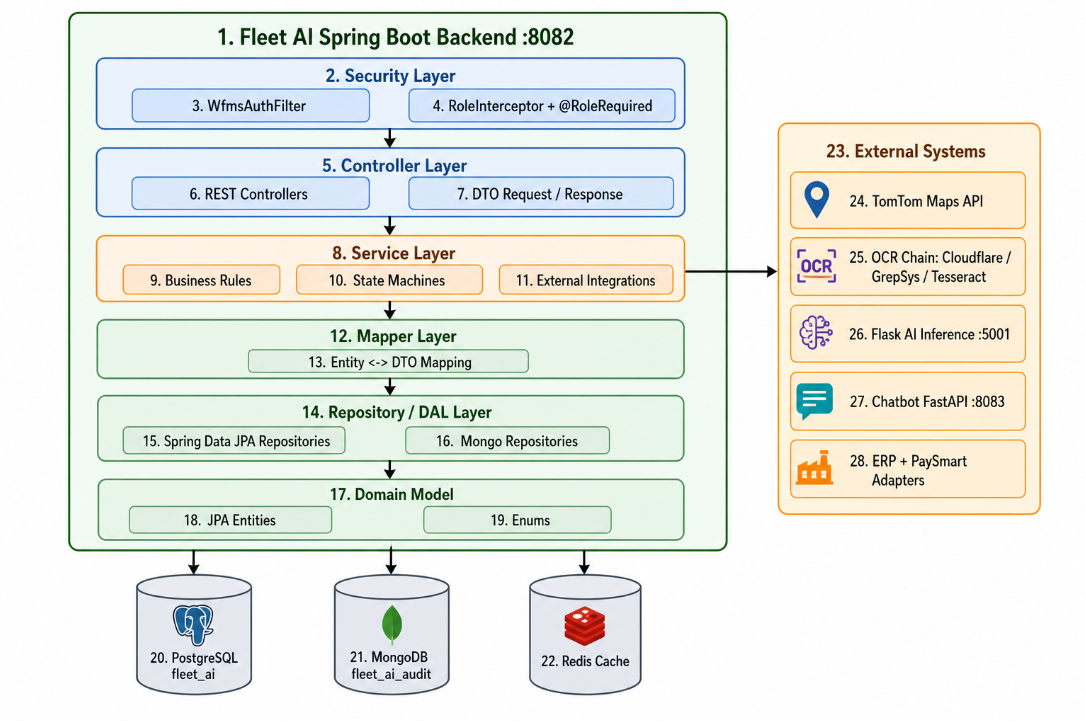
\includegraphics[width=\linewidth]{img/architecture/backend_architecture}
\caption{Architecture N-tiers en couches du back-end Fleet~AI}
\label{fig:archi-backend}
\end{figure}

\begin{itemize}
    \item[$\bullet$] \textbf{Controller :} Expose les endpoints REST, extrait le contexte WFMS et délègue aux services.
    \item[$\bullet$] \textbf{Service :} Contient la logique métier, les validations et les règles de gestion.
    \item[$\bullet$] \textbf{Repository :} Interface Spring Data JPA pour l'accès aux données relationnelles (PostgreSQL).
    \item[$\bullet$] \textbf{Entity :} Classes JPA avec héritage JOINED (FleetUser $\rightarrow$ Chauffeur, Administrateur, Manager, Planificateur).
    \item[$\bullet$] \textbf{DTO :} Objets de transfert séparés en \texttt{request/} et \texttt{response/} pour découpler l'API du modèle interne.
    \item[$\bullet$] \textbf{Mapper :} Convertit les entités JPA en DTOs et inversement.
    \item[$\bullet$] \textbf{Security :} Filtre d'authentification WFMS (\texttt{WfmsAuthFilter}) et intercepteur RBAC (\texttt{@RoleRequired}).
\end{itemize}

% ------ FRONTEND ARCHITECTURE ------
\subsection{Architecture du Front-end (Angular)}

Le front-end Angular~19 suit une \textbf{architecture modulaire} structurée en trois couches principales : \textbf{Core}, \textbf{Modules} (fonctionnalités métier) et \textbf{Shared} (composants réutilisables). Chaque module métier est découpé en sous-dossiers \texttt{data-access/} (services et modèles) et \texttt{pages/} (composants de vue).

\begin{figure}[H]
\centering
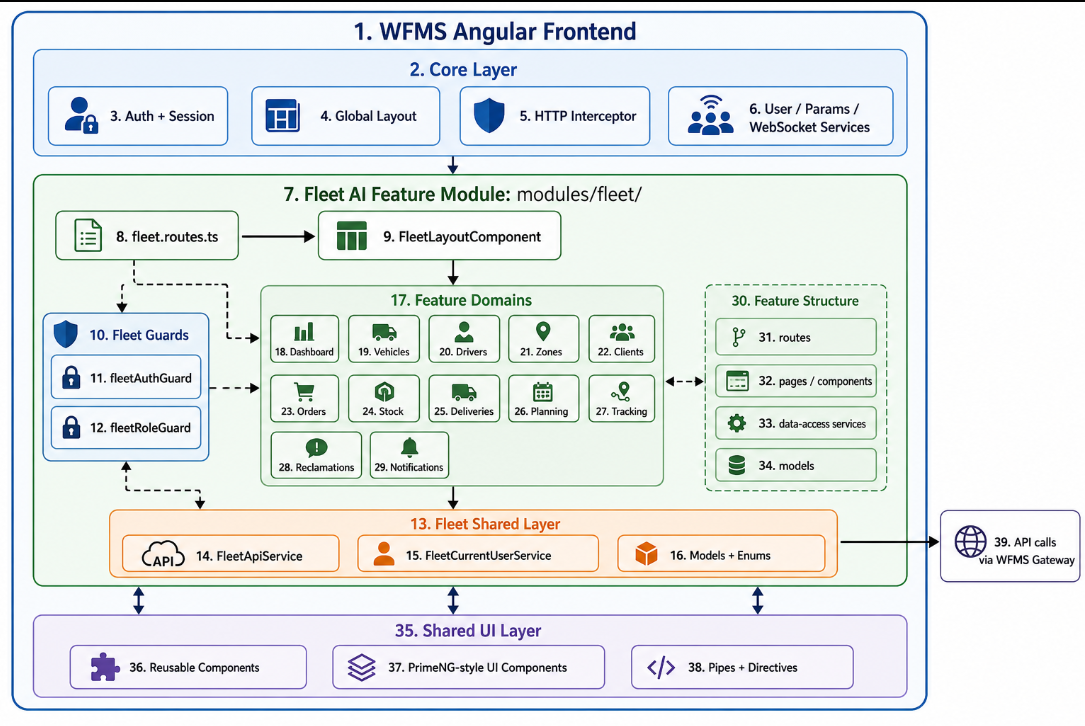
\includegraphics[width=\linewidth]{img/architecture/angular_frontend_architecture}
\caption{Architecture modulaire du front-end Angular~19}
\label{fig:archi-frontend}
\end{figure}

% ------ MOBILE ARCHITECTURE ------
\subsection{Architecture Mobile (Flutter -- MVVM)}

L'application mobile Flutter adopte le pattern \textbf{MVVM} (Model--View--ViewModel) qui sépare clairement la logique de présentation de la logique métier et de l'accès aux données.

\begin{figure}[H]
\centering
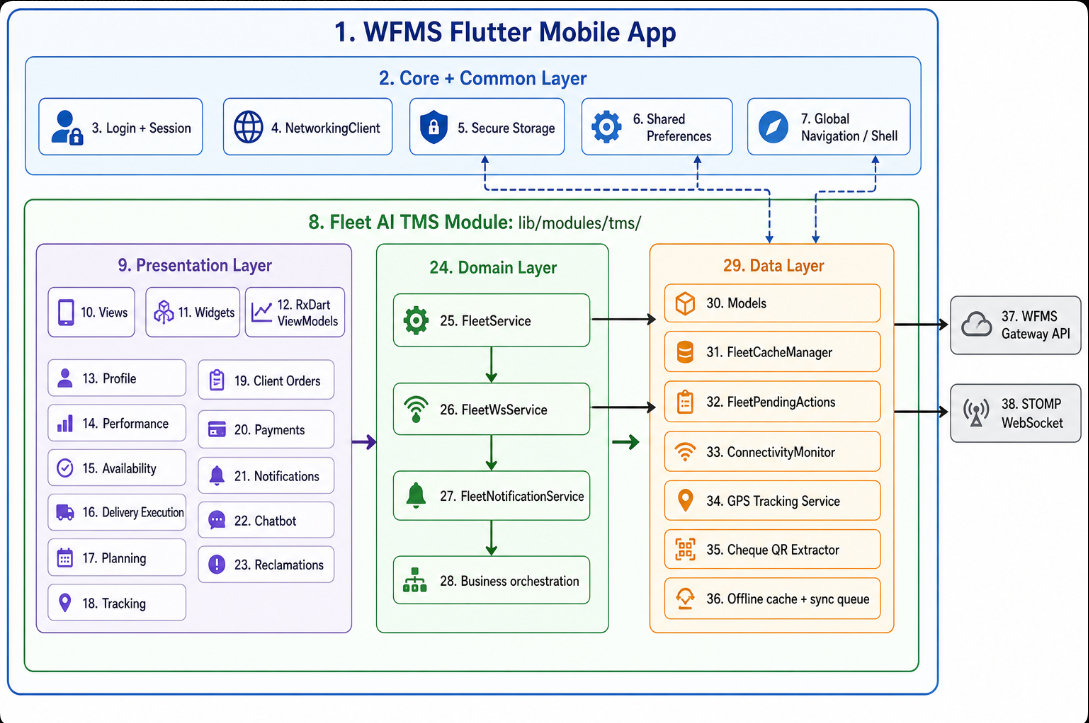
\includegraphics[width=\linewidth]{img/architecture/flutter_mvvm_architecture}
\caption{Architecture MVVM de l'application mobile Flutter}
\label{fig:archi-mobile}
\end{figure}

\begin{itemize}
    \item[$\bullet$] \textbf{View :} Les widgets Flutter affichent l'interface utilisateur et capturent les interactions de l'utilisateur (chauffeur).
    \item[$\bullet$] \textbf{ViewModel :} Gère l'état de l'application, transforme les données du modèle et notifie la vue des changements via le data binding.
    \item[$\bullet$] \textbf{Model :} Contient les entités de données, les repositories qui encapsulent l'accès aux API REST (via la passerelle WFMS) et le stockage local pour le mode hors ligne.
\end{itemize}



\section*{Conclusion}
\addcontentsline{toc}{section}{Conclusion}
La méthodologie Scrum a permis une grande flexibilité tout au long du projet. L'architecture N-Tiers associée à la passerelle WFMS offre une structure robuste pour accueillir l'ensemble des fonctionnalités que nous décrirons dans les prochains chapitres.


% ---- Chapitre 4 : Sprint 1 ----
\chapter{Sprint 1 : Fondation \& Gestion des Ressources}

\section*{Introduction}
\addcontentsline{toc}{section}{Introduction}
Le Sprint~1 constitue la fondation technique de Fleet~AI. Il met en place les mécanismes d'authentification unifiée via la passerelle WFMS et le contrôle d'accès par rôles, garantissant que chaque acteur n'accède qu'aux fonctionnalités qui lui sont attribuées. Les référentiels opérationnels — utilisateurs, véhicules, chauffeurs et zones géographiques — sont créés et gérés depuis l'interface web. Le journal d'audit et les sauvegardes assurent la traçabilité et la sécurité des données. En parallèle, l'application mobile Flutter est initialisée pour les Chauffeurs, leur permettant de se connecter, de consulter leurs indicateurs de performance et de déclarer leur disponibilité. Ce premier sprint pose les bases sur lesquelles tous les sprints suivants vont s'appuyer.

\clearpage

\section{Sprint Backlog}

\textbf{Objectif du sprint :} L'objectif est de mettre en place l'authentification WFMS, le contrôle d'accès par rôles et les référentiels de base — utilisateurs, véhicules, chauffeurs, zones — ainsi que le journal d'audit, les sauvegardes et l'application mobile Chauffeur.

\definecolor{headerbg}{HTML}{d5f5e3}
\setlength{\arrayrulewidth}{1pt}

Les story points (SP) sont estimés par l'équipe de développement selon la suite de Fibonacci (1, 2, 3, 5, 8, 13, \ldots). Chaque valeur reflète la \textbf{complexité fonctionnelle}, l'\textbf{effort} et le \textbf{risque} associé à la User Story, et non une durée en heures. L'échelle retenue est : 1--2 (tâche simple, déjà maîtrisée), 3--5 (complexité modérée), 8--13 (tâche complexe ou comportant une forte incertitude).

\begin{longtable}{|>{\raggedright\arraybackslash}p{4.2cm}|>{\raggedright\arraybackslash}p{4.8cm}|>{\raggedright\arraybackslash}p{4.5cm}|c|}
\hline
\rowcolor{headerbg}
\textbf{User Story} & \textbf{Tâche} & \textbf{Critères d'acceptation} & \textbf{\rotatebox{90}{SP}} \\
\hline
\endfirsthead
\hline
\rowcolor{headerbg}
\textbf{User Story} & \textbf{Tâche} & \textbf{Critères d'acceptation} & \textbf{\rotatebox{90}{SP}} \\
\hline
\endhead
\hline
\endfoot

%------ US-001 ------
\multirow{2}{=}{En tant qu'utilisateur, je veux me connecter avec mes identifiants habituels afin d'accéder aux fonctionnalités Fleet~AI correspondant à mon rôle.}
& Mettre en place la vérification des identifiants à la connexion afin de valider l'accès de l'utilisateur. & L'utilisateur peut se connecter avec ses identifiants habituels ; un message clair s'affiche en cas d'erreur. & 3 \\
\cline{2-4}
& Rediriger chaque utilisateur vers son espace dédié selon son rôle après connexion réussie. & Chaque rôle accède à son interface dédiée après authentification. & 2 \\
\hline

%------ US-002 ------
\multirow{2}{=}{En tant qu'Administrateur, je veux que les droits de chaque utilisateur soient contrôlés à chaque accès afin que chacun n'utilise que les fonctionnalités autorisées par son rôle.}
& Contrôler les droits d'accès de l'utilisateur à chaque action sensible selon son rôle. & Un utilisateur sans les droits requis se voit refuser l'accès avec un message explicite ; son rôle détermine ses permissions. & 3 \\
\cline{2-4}
& Valider que chaque rôle accède uniquement aux fonctionnalités qui lui sont autorisées. & Les accès autorisés et refusés sont cohérents avec les droits définis par rôle pour tous les profils du système. & 2 \\
\hline

%------ US-003 ------
\multirow{2}{=}{En tant qu'Administrateur, je veux gérer les comptes utilisateurs afin de contrôler les accès au système.}
& Permettre à l'Administrateur de créer, modifier et désactiver des comptes utilisateurs selon leur rôle. & Le CRUD complet fonctionne ; un compte désactivé ne peut plus accéder au système. & 3 \\
\cline{2-4}
& Mettre à disposition de l'Administrateur une interface de gestion des comptes avec liste paginée et formulaires. & La liste des utilisateurs est consultable avec filtres ; les formulaires de création et d'édition sont fonctionnels. & 2 \\
\hline

%------ US-004 ------
\multirow{2}{=}{En tant qu'Administrateur, je veux assigner un rôle à chaque utilisateur afin de définir ses permissions.}
& Associer un rôle unique à chaque utilisateur lors de sa création afin de définir ses droits dans le système. & Le rôle attribué détermine les fonctionnalités accessibles ; les permissions sont vérifiées à chaque action. & 3 \\
\cline{2-4}
& Présenter la liste des rôles disponibles dans le formulaire de création d'utilisateur avec sélection obligatoire. & La liste des rôles est affichée ; la sélection est obligatoire avant validation du formulaire. & 2 \\
\hline

%------ US-005 ------
\multirow{2}{=}{En tant qu'Administrateur, je veux gérer les zones géographiques de livraison afin de structurer les opérations par région.}
& Permettre la création et la modification de zones géographiques définies par des polygones sur carte. & Les zones sont définies par polygone sur carte ; leur surface et périmètre sont calculés automatiquement. & 3 \\
\cline{2-4}
& Mettre à disposition une carte interactive permettant à l'Administrateur de dessiner et modifier les zones. & La carte interactive permet la création et l'édition des polygones de zones géographiques. & 2 \\
\hline

%------ US-006 ------
\multirow{2}{=}{En tant qu'Administrateur, je veux consulter le journal d'audit du système afin de tracer toutes les actions critiques.}
& Enregistrer automatiquement toutes les actions critiques (entité concernée, acteur, date, type d'action). & Les entrées du journal sont enregistrées pour chaque action ; filtrables par date, utilisateur, action et entité. & 3 \\
\cline{2-4}
& Mettre à disposition de l'Administrateur une interface de consultation du journal avec pagination et filtres. & La liste des entrées est paginée ; les filtres combinés fonctionnent correctement. & 2 \\
\hline

%------ US-007 ------
\multirow{2}{=}{En tant qu'Administrateur, je veux déclencher des sauvegardes des données afin de protéger les informations du système.}
& Permettre à l'Administrateur de déclencher une sauvegarde complète de la base de données. & La sauvegarde est effectuée et archivée avec horodatage ; l'Administrateur peut confirmer son succès. & 2 \\
\cline{2-4}
& Afficher à l'Administrateur l'historique des sauvegardes avec leur statut. & L'historique des sauvegardes est consultable avec statut mis à jour (en cours, terminée, échouée). & 1 \\
\hline

%------ US-008 ------
\multirow{2}{=}{En tant qu'Administrateur, je veux consulter le tableau de bord avec les statistiques générales afin de superviser l'état du système.}
& Calculer et exposer les indicateurs clés du système (utilisateurs actifs, véhicules, chauffeurs, zones, coûts). & Les indicateurs affichés sont corrects et filtrables par période. & 3 \\
\cline{2-4}
& Présenter les indicateurs et tendances sous forme de graphiques et de tableau de bord visuel. & Le tableau de bord affiche les KPIs, les tendances de coûts et l'activité récente. & 2 \\
\hline

%------ US-009 ------
\multirow{2}{=}{En tant que Planificateur, je veux consulter la liste des véhicules avec leur statut afin de connaître les ressources disponibles.}
& Mettre à disposition du Planificateur la liste des véhicules filtrée par statut et par zone. & La liste affiche le statut, la capacité (poids/volume), le kilométrage et la zone ; pagination intégrée. & 2 \\
\cline{2-4}
& Permettre au Planificateur de filtrer et trier la liste des véhicules selon ses besoins. & La liste des véhicules s'affiche avec filtres fonctionnels par statut et par zone. & 1 \\
\hline

%------ US-010 ------
\multirow{2}{=}{En tant qu'Administrateur, je veux gérer les véhicules afin de maintenir le référentiel à jour.}
& Permettre à l'Administrateur de créer, modifier et supprimer des véhicules, avec protection contre la suppression d'un véhicule en mission. & Un véhicule en mission ne peut être supprimé ; la suppression est logique et réversible. & 2 \\
\cline{2-4}
& Mettre à disposition de l'Administrateur un formulaire de création et modification des véhicules avec validation des champs. & Le formulaire valide tous les champs obligatoires ; la liste se met à jour après sauvegarde. & 1 \\
\hline

%------ US-011 ------
\multirow{2}{=}{En tant que Planificateur, je veux marquer un véhicule en maintenance afin de le retirer temporairement de la planification.}
& Permettre au Planificateur de changer le statut d'un véhicule vers « En maintenance », avec enregistrement dans le journal d'audit. & Le changement est immédiat ; le véhicule en maintenance est exclu des affectations. & 2 \\
\cline{2-4}
& Afficher une demande de confirmation au Planificateur avant le changement de statut du véhicule. & La confirmation est demandée avant l'action ; le statut est mis à jour dans la liste. & 1 \\
\hline

%------ US-012 ------
\multirow{2}{=}{En tant que Manager, je veux consulter le taux d'utilisation des véhicules afin d'optimiser la flotte.}
& Calculer le taux d'utilisation des véhicules à partir de leur historique de kilométrage. & Le taux est calculé par véhicule et de manière globale sur la période sélectionnée. & 3 \\
\cline{2-4}
& Présenter le taux d'utilisation sous forme de graphique par véhicule avec sélection de période. & Le graphique s'affiche par véhicule avec sélection de la période. & 2 \\
\hline

%------ US-013 ------
\multirow{2}{=}{En tant que Manager, je veux consulter les coûts par véhicule afin de suivre les dépenses opérationnelles.}
& Calculer et exposer les coûts par véhicule ventilés par catégorie (carburant, entretien, assurance). & Les coûts sont ventilés par catégorie ; les tendances mensuelles sont calculées. & 3 \\
\cline{2-4}
& Présenter les coûts sous forme de graphique et identifier les 5 véhicules les plus coûteux. & Le tableau de bord affiche les 5 véhicules les plus coûteux avec graphique mensuel. & 2 \\
\hline

%------ US-014 ------
\multirow{2}{=}{En tant que Planificateur, je veux consulter la disponibilité des chauffeurs afin de planifier les affectations.}
& Mettre à disposition du Planificateur un calendrier de disponibilité des chauffeurs avec filtres par type et par zone. & Le calendrier affiche les disponibilités par type (disponible, congé, mission) et par zone. & 3 \\
\cline{2-4}
& Permettre au Planificateur de filtrer les disponibilités par plage de dates et par zone. & La vue calendrier filtrée par date et par zone fonctionne correctement. & 2 \\
\hline

%------ US-015 ------
\multirow{2}{=}{En tant que Planificateur, je veux consulter les performances des chauffeurs afin de guider les affectations.}
& Calculer les indicateurs de performance des chauffeurs (taux de livraison, ponctualité, notation moyenne) selon les coefficients configurés. & Les indicateurs sont calculés selon les coefficients définis par l'Administrateur et affichés dans la fiche du chauffeur. & 3 \\
\cline{2-4}
& Présenter les indicateurs de performance du chauffeur avec des repères visuels dans son profil. & La fiche chauffeur affiche les indicateurs avec des repères visuels de niveau. & 2 \\
\hline

%------ US-016 ------
\multirow{2}{=}{En tant que Manager, je veux consulter le classement des chauffeurs afin d'identifier les plus et les moins performants.}
& Calculer et présenter le classement des chauffeurs selon leur score global pondéré. & Le classement est trié par score global ; accessible depuis le tableau de bord. & 2 \\
\cline{2-4}
& Afficher le classement des chauffeurs avec des indicateurs permettant d'identifier les plus et moins performants. & Le classement s'affiche avec indicateurs colorés de performance. & 1 \\
\hline

%------ US-017 ------
\multirow{2}{=}{En tant qu'Administrateur, je veux configurer les indicateurs de performance des chauffeurs afin d'adapter le calcul du score global.}
& Permettre à l'Administrateur de modifier les 3 coefficients de performance des chauffeurs ; toute modification est enregistrée dans le journal d'audit. & Les modifications sont tracées dans le journal d'audit. & 2 \\
\cline{2-4}
& Présenter un formulaire de configuration des coefficients avec validation de leur cohérence. & Le formulaire vérifie que les coefficients sont cohérents et la somme correcte avant enregistrement. & 1 \\
\hline

%------ US-018 ------
\multirow{2}{=}{En tant que Chauffeur, je veux me connecter à l'application mobile afin d'accéder à mes fonctionnalités Fleet~AI.}
& Permettre au Chauffeur de se connecter à l'application mobile avec ses identifiants habituels et de rester authentifié. & La connexion mobile fonctionne ; l'application Fleet~AI est accessible depuis l'application après authentification. & 3 \\
\cline{2-4}
& Permettre au Chauffeur d'accéder à l'application Fleet~AI depuis le menu de navigation de l'application mobile. & L'application Fleet~AI est accessible depuis le menu de navigation après connexion. & 2 \\
\hline

%------ US-019 ------
\multirow{2}{=}{En tant que Chauffeur, je veux consulter mes indicateurs de performance depuis l'application mobile afin de suivre mon activité.}
& Présenter au Chauffeur ses indicateurs de performance personnels sur l'application mobile. & L'écran affiche les indicateurs avec graphiques ; les coefficients de pondération sont ceux configurés par l'Administrateur. & 3 \\
\cline{2-4}
& Afficher les graphiques de performance sur l'application mobile de manière lisible. & Les graphiques de performance s'affichent correctement sur l'application mobile. & 2 \\
\hline

%------ US-020 ------
\multirow{2}{=}{En tant que Chauffeur, je veux déclarer ma disponibilité depuis l'application mobile afin de signaler mes périodes de présence et d'absence.}
& Permettre au Chauffeur de déclarer ses périodes de disponibilité ou d'absence depuis l'application mobile (types : disponible, congé, formation, mission). & La déclaration est enregistrée ; les chevauchements de créneaux sont détectés et signalés. & 3 \\
\cline{2-4}
& Valider les règles de disponibilité selon le type de contrat du chauffeur (officiel ou prestataire). & Les chauffeurs officiels ne peuvent déclarer que des absences ; les prestataires peuvent déclarer leur disponibilité. & 2 \\
\hline

%------ US-113/114 ------
\multirow{2}{=}{En tant qu'utilisateur, je veux configurer mes préférences de notifications et consulter mon historique depuis mon application.}
& Permettre à l'utilisateur de choisir ses canaux de notification (dans l'application, par email) par type d'événement. & L'utilisateur peut choisir les canaux par type d'événement et sauvegarder ses préférences. & 2 \\
\cline{2-4}
& Permettre à l'utilisateur de consulter l'historique de ses notifications depuis l'application web ou mobile. & Les préférences sont sauvegardées ; l'historique des notifications est accessible. & 1 \\
\hline

\caption{Sprint Backlog du Sprint 1 --- Fondation \& Gestion des Ressources (20 stories, 76 SP)}
\end{longtable}
\setlength{\arrayrulewidth}{0.4pt}


\section{Conception}

\subsection{Diagramme de cas d'utilisation}

\begin{figure}[H]
\centering
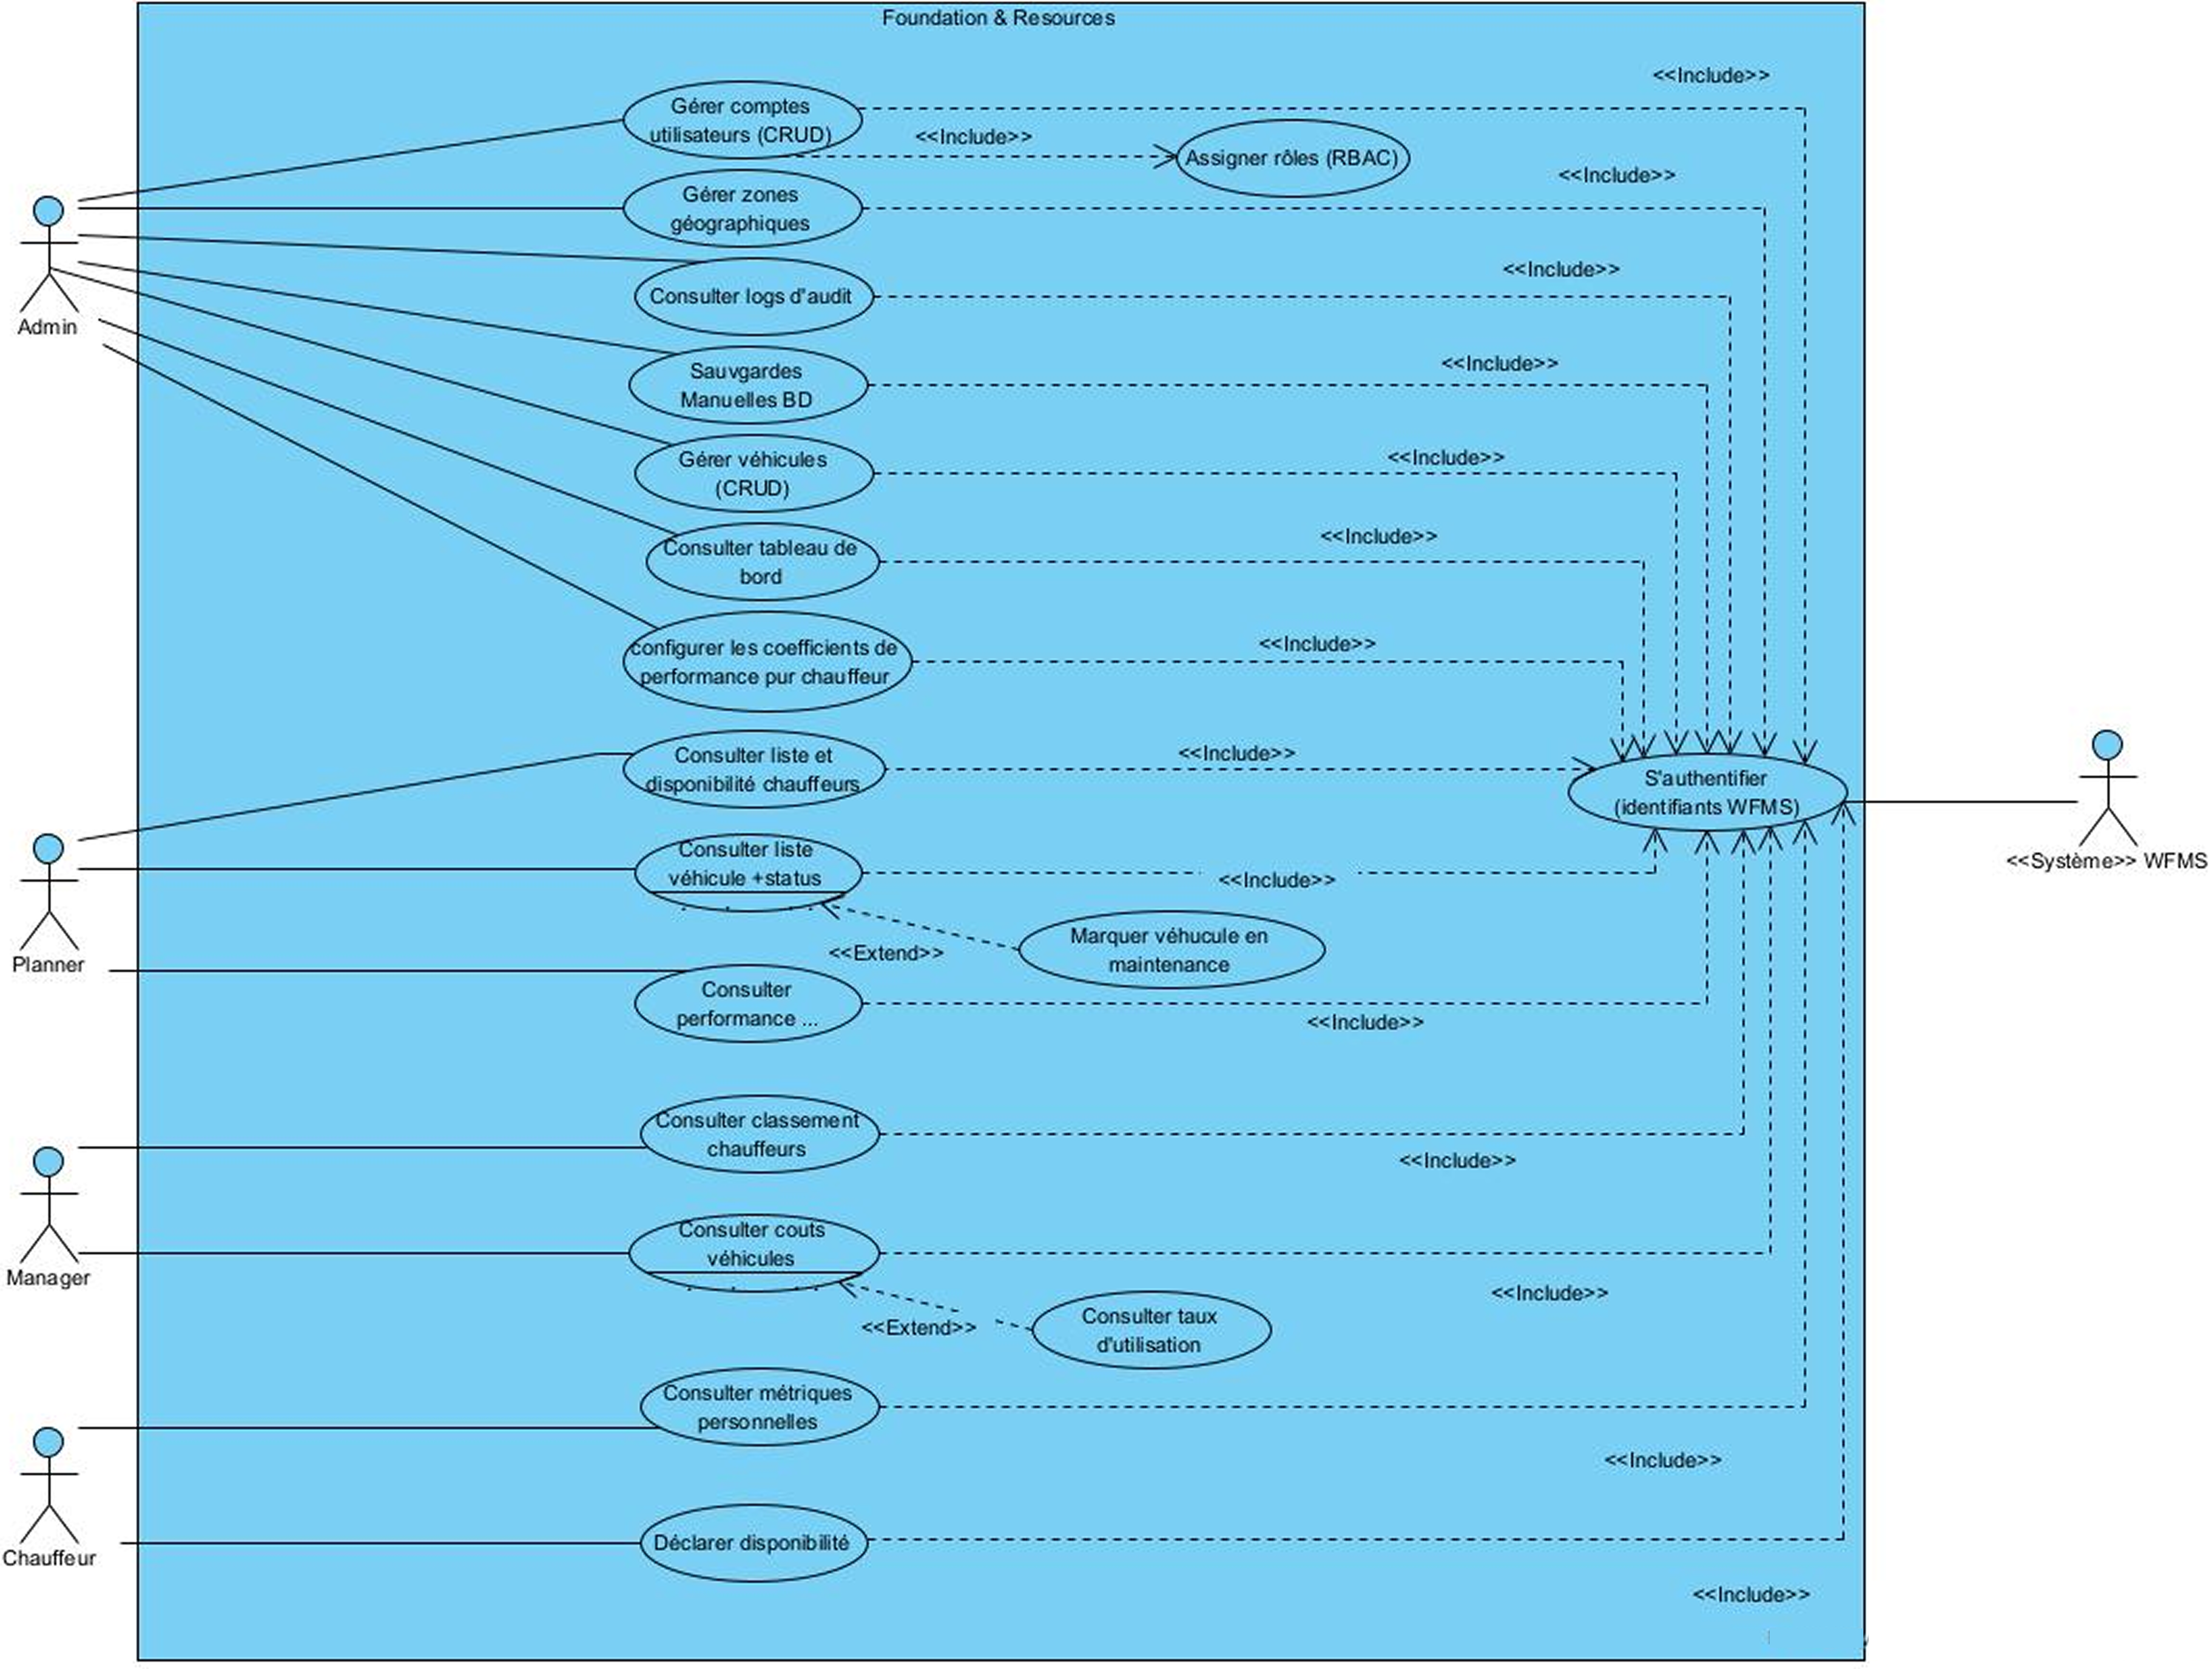
\includegraphics[width=\linewidth, height=0.85\textheight, keepaspectratio]{img/diagrammes/sprint_1_usecase}
\caption{Diagramme de cas d'utilisation du Sprint 1}
\label{fig:cas-utilisation-sp1}
\end{figure}

\subsection{Description textuelle}

\captionsetup[longtable]{justification=centering}
\setlength{\arrayrulewidth}{1pt}
\begin{longtable}{|p{4cm}|p{11cm}|}
\hline
\rowcolor{headerbg}
\textbf{Élément} & \textbf{Description} \\
\hline
\textbf{Titre} & Gérer les chauffeurs \\
\hline
\textbf{Acteurs} & Administrateur, Planificateur \\
\hline
\textbf{Objectif} & Permettre la gestion complète des profils chauffeurs : création, consultation, modification et suppression depuis l'application web. \\
\hline
\textbf{Précondition} & L'utilisateur est authentifié via WFMS et possède le rôle Administrateur ou Planificateur. \\
\hline
\textbf{Postcondition} & L'opération est enregistrée dans le journal d'audit MongoDB. \\
\hline
\textbf{Scénario nominal} &
\begin{enumerate}[start=1, label=\arabic*.]
    \item L'utilisateur accède à la page « Chauffeurs » depuis le menu latéral.
    \item Le système affiche la liste paginée des chauffeurs (nom, prénom, zone, permis, score).
    \item Pour ajouter : l'utilisateur clique sur « Ajouter », remplit le formulaire et valide.
    \item Pour modifier : l'utilisateur clique sur l'icône d'édition, modifie les champs et valide.
    \item Pour supprimer : l'utilisateur clique sur l'icône de suppression et confirme.
    \item Le système enregistre l'opération et met à jour l'affichage.
\end{enumerate} \\
\hline
\textbf{Scénario alternatif} &
\begin{enumerate}[start=1, label=\arabic*.]
    \item Si les données sont invalides (permis expiré, champ vide), un message d'erreur est affiché.
    \item Si l'utilisateur n'a pas le rôle requis, le système retourne une erreur 403.
\end{enumerate} \\
\hline
\caption{Description textuelle --- Gérer les chauffeurs (Sprint 1)}
\end{longtable}
\setlength{\arrayrulewidth}{0.4pt}

\subsection{Diagramme de classes}

\newpage
\thispagestyle{empty}
\begin{landscape}
\begin{figure}[H]
\centering
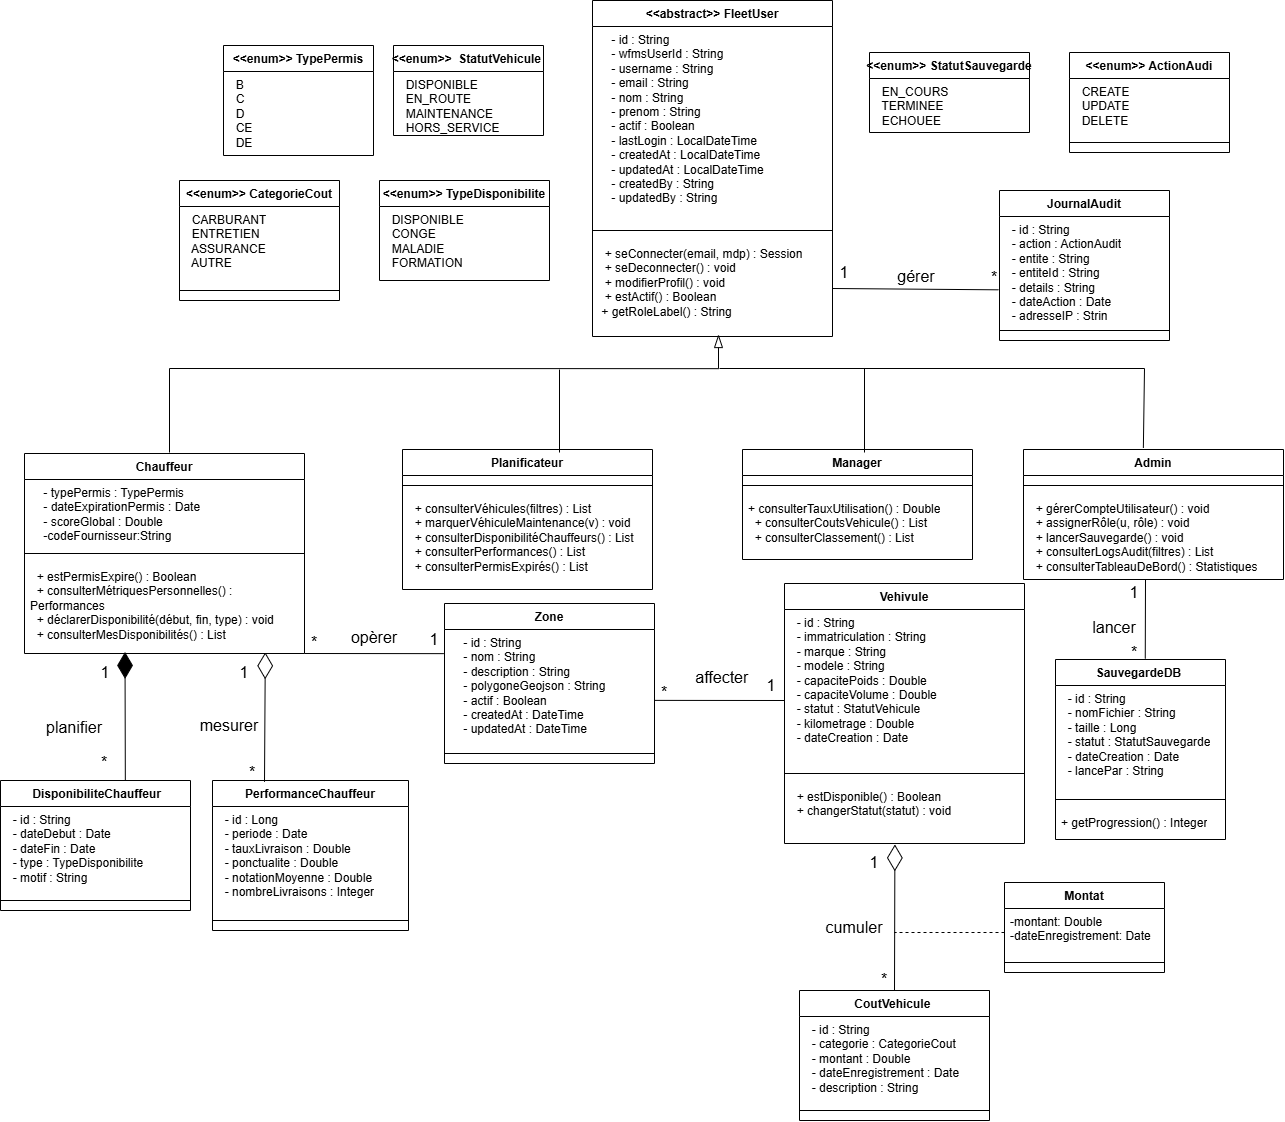
\includegraphics[width=\linewidth, height=0.95\textheight, keepaspectratio]{img/diagrammes/DiagrammeCorrige}
\caption{Diagramme de classes du Sprint 1}
\label{fig:class-diagram-sp1}
\end{figure}
\end{landscape}

% =============================================================
\section{Réalisation}
% =============================================================

\subsection{Sécurité : Authentification et RBAC}
La sécurité applicative repose sur deux composants :
\begin{itemize}
    \item[$\bullet$] \textbf{WfmsAuthFilter :} Filtre qui intercepte les requêtes, déchiffre le token RSA WFMS et injecte l'identité de l'utilisateur.
    \item[$\bullet$] \textbf{RoleInterceptor + @RoleRequired :} Vérifie le rôle requis via l'héritage polymorphique des entités FleetUser.
\end{itemize}

\subsection{Tableau de bord et authentification}

L'authentification passe par WFMS. Chaque acteur est redirigé vers son tableau de bord avec KPIs en temps réel.

\begin{figure}[H]
\centering
\IfFileExists{img/capture/web/sp1_dashboard_composite.png}{%
  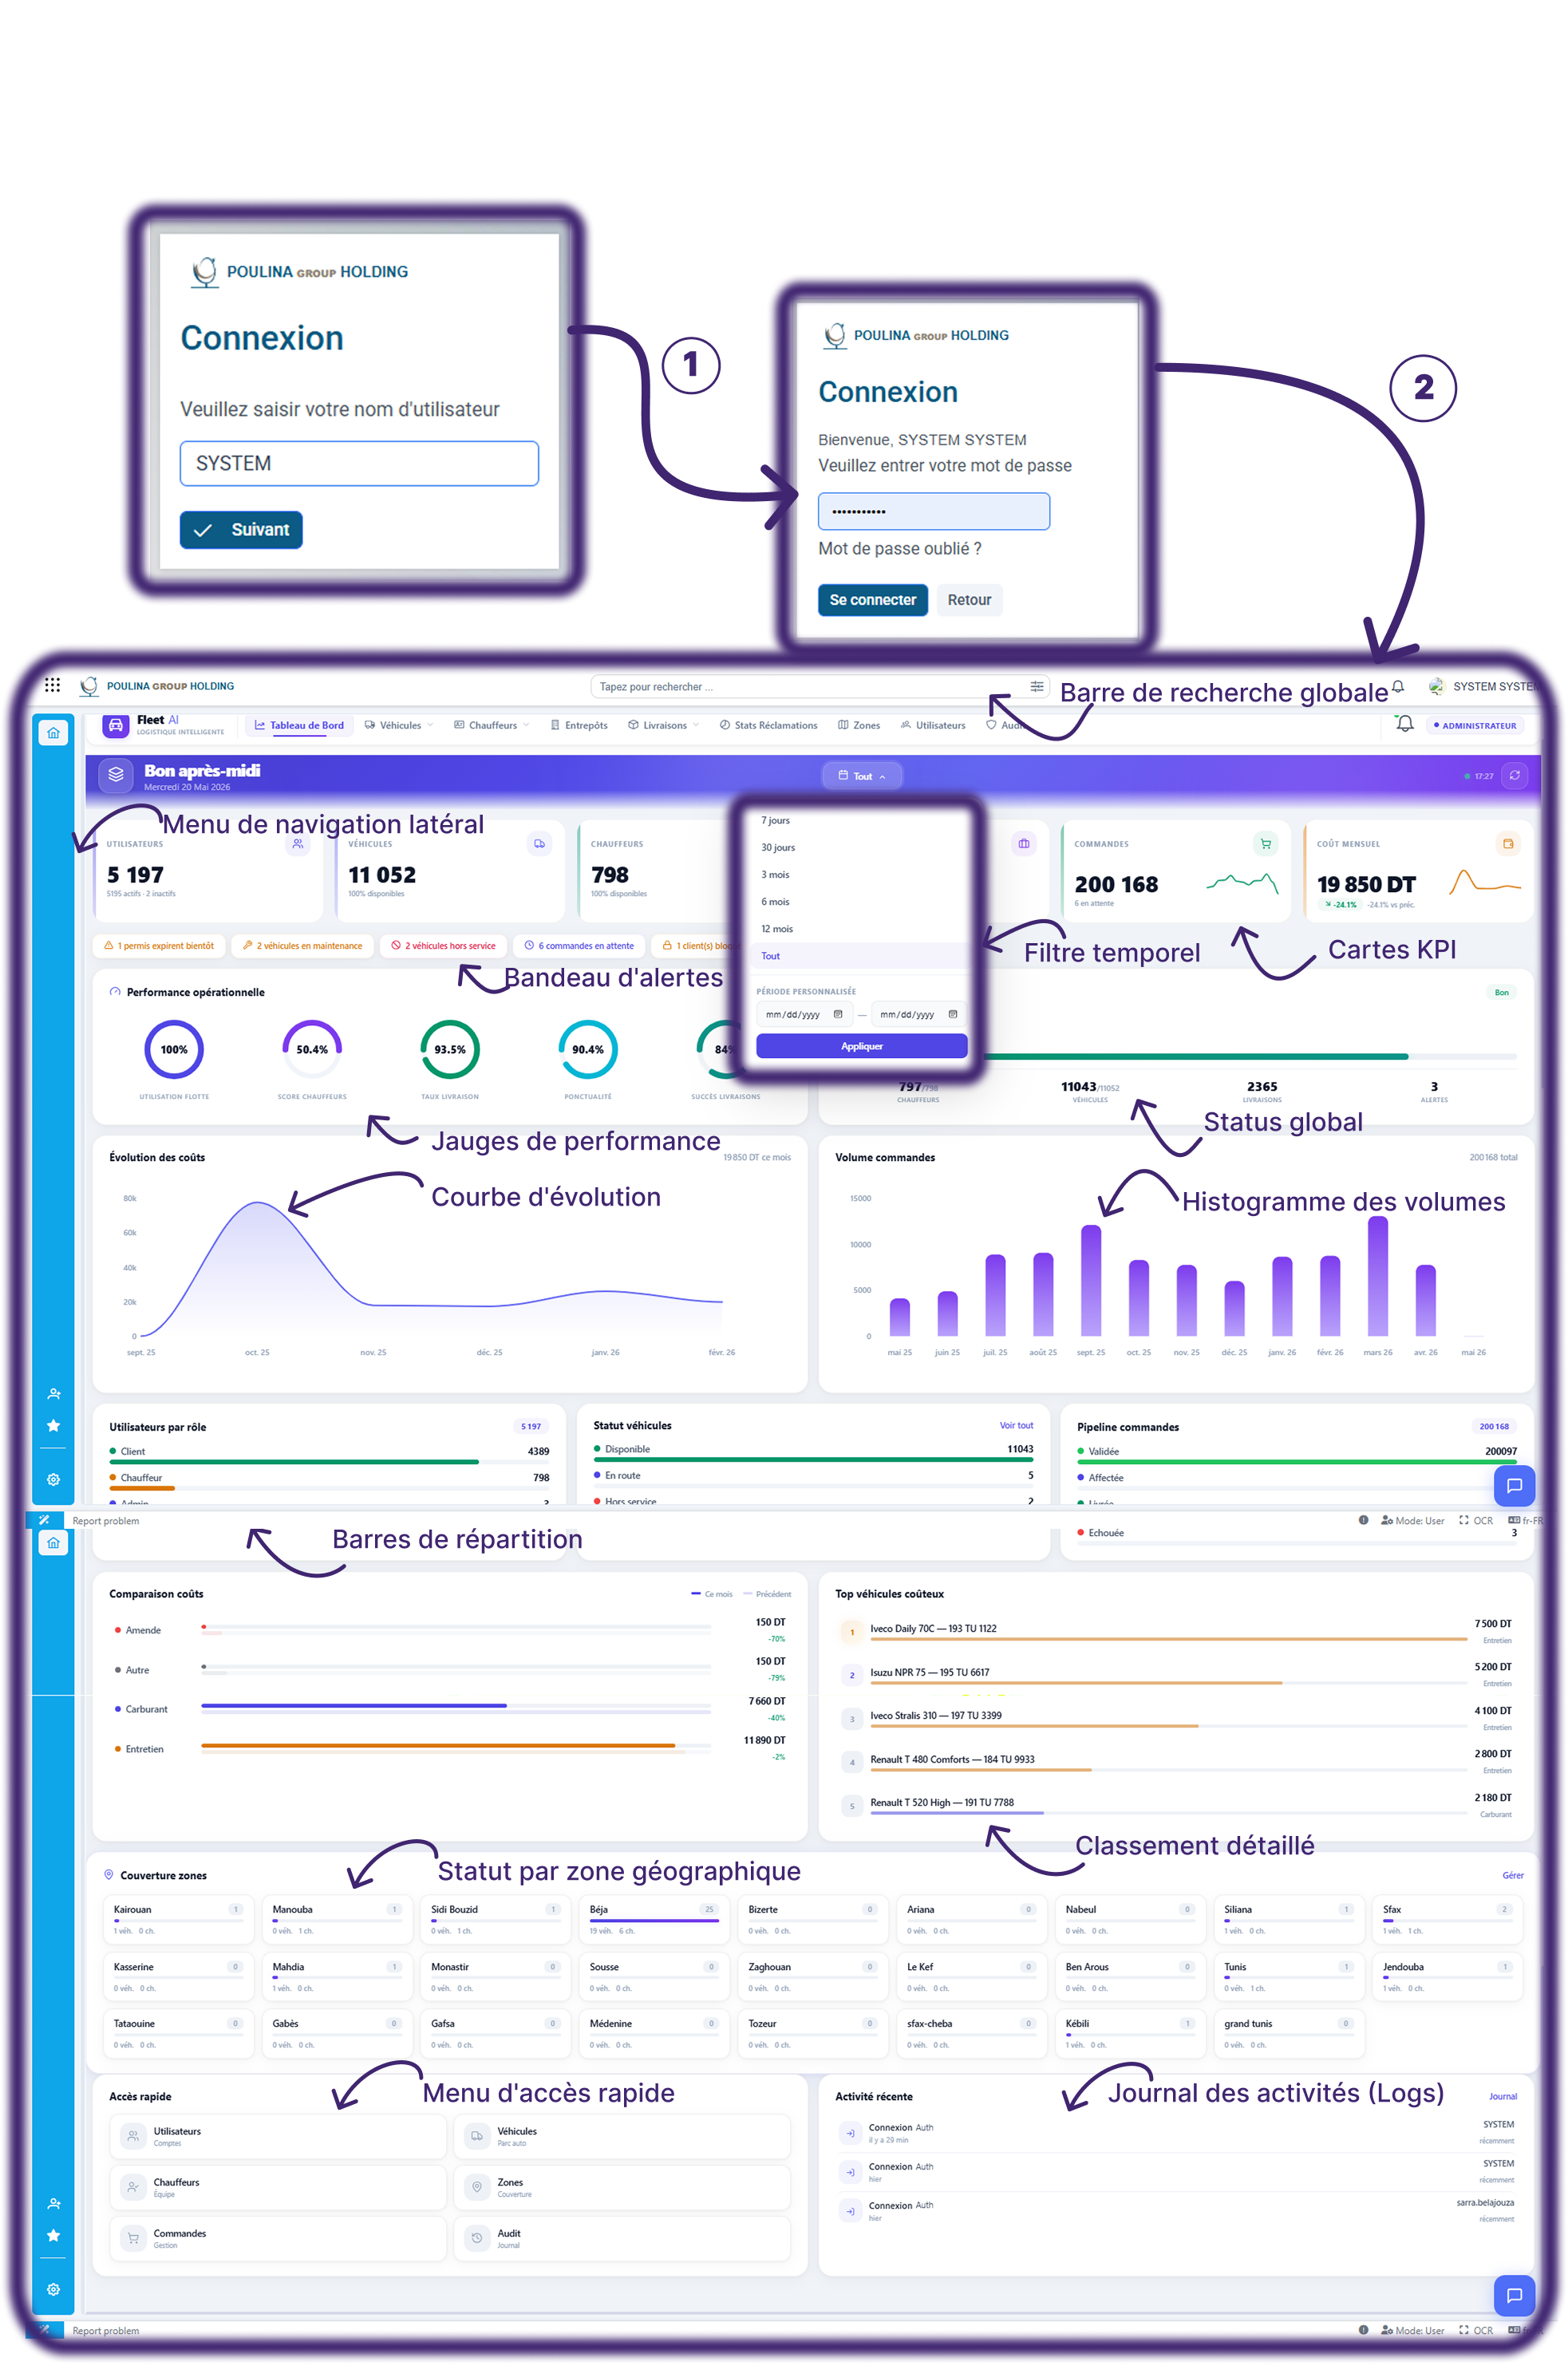
\includegraphics[width=\linewidth, keepaspectratio]{img/capture/web/sp1_dashboard_composite}%
}{%
  \fbox{\parbox{0.9\linewidth}{\centering\vspace{4cm}\textit{[img/sp1\_dashboard\_composite]}\vspace{4cm}}}%
}
\caption{Tableau de bord Fleet~AI : KPIs administrateur et connexion WFMS}
\label{fig:sp1-dashboard}
\end{figure}

\subsection{Gestion des utilisateurs}

L'Administrateur crée, modifie et désactive des comptes utilisateurs, en assignant l'un des six rôles disponibles : AD, MG, PL, CH, REC, CL. Un compte désactivé perd immédiatement tout accès.

\begin{figure}[H]
\centering
\IfFileExists{img/capture/web/sp1_users_composite.png}{%
  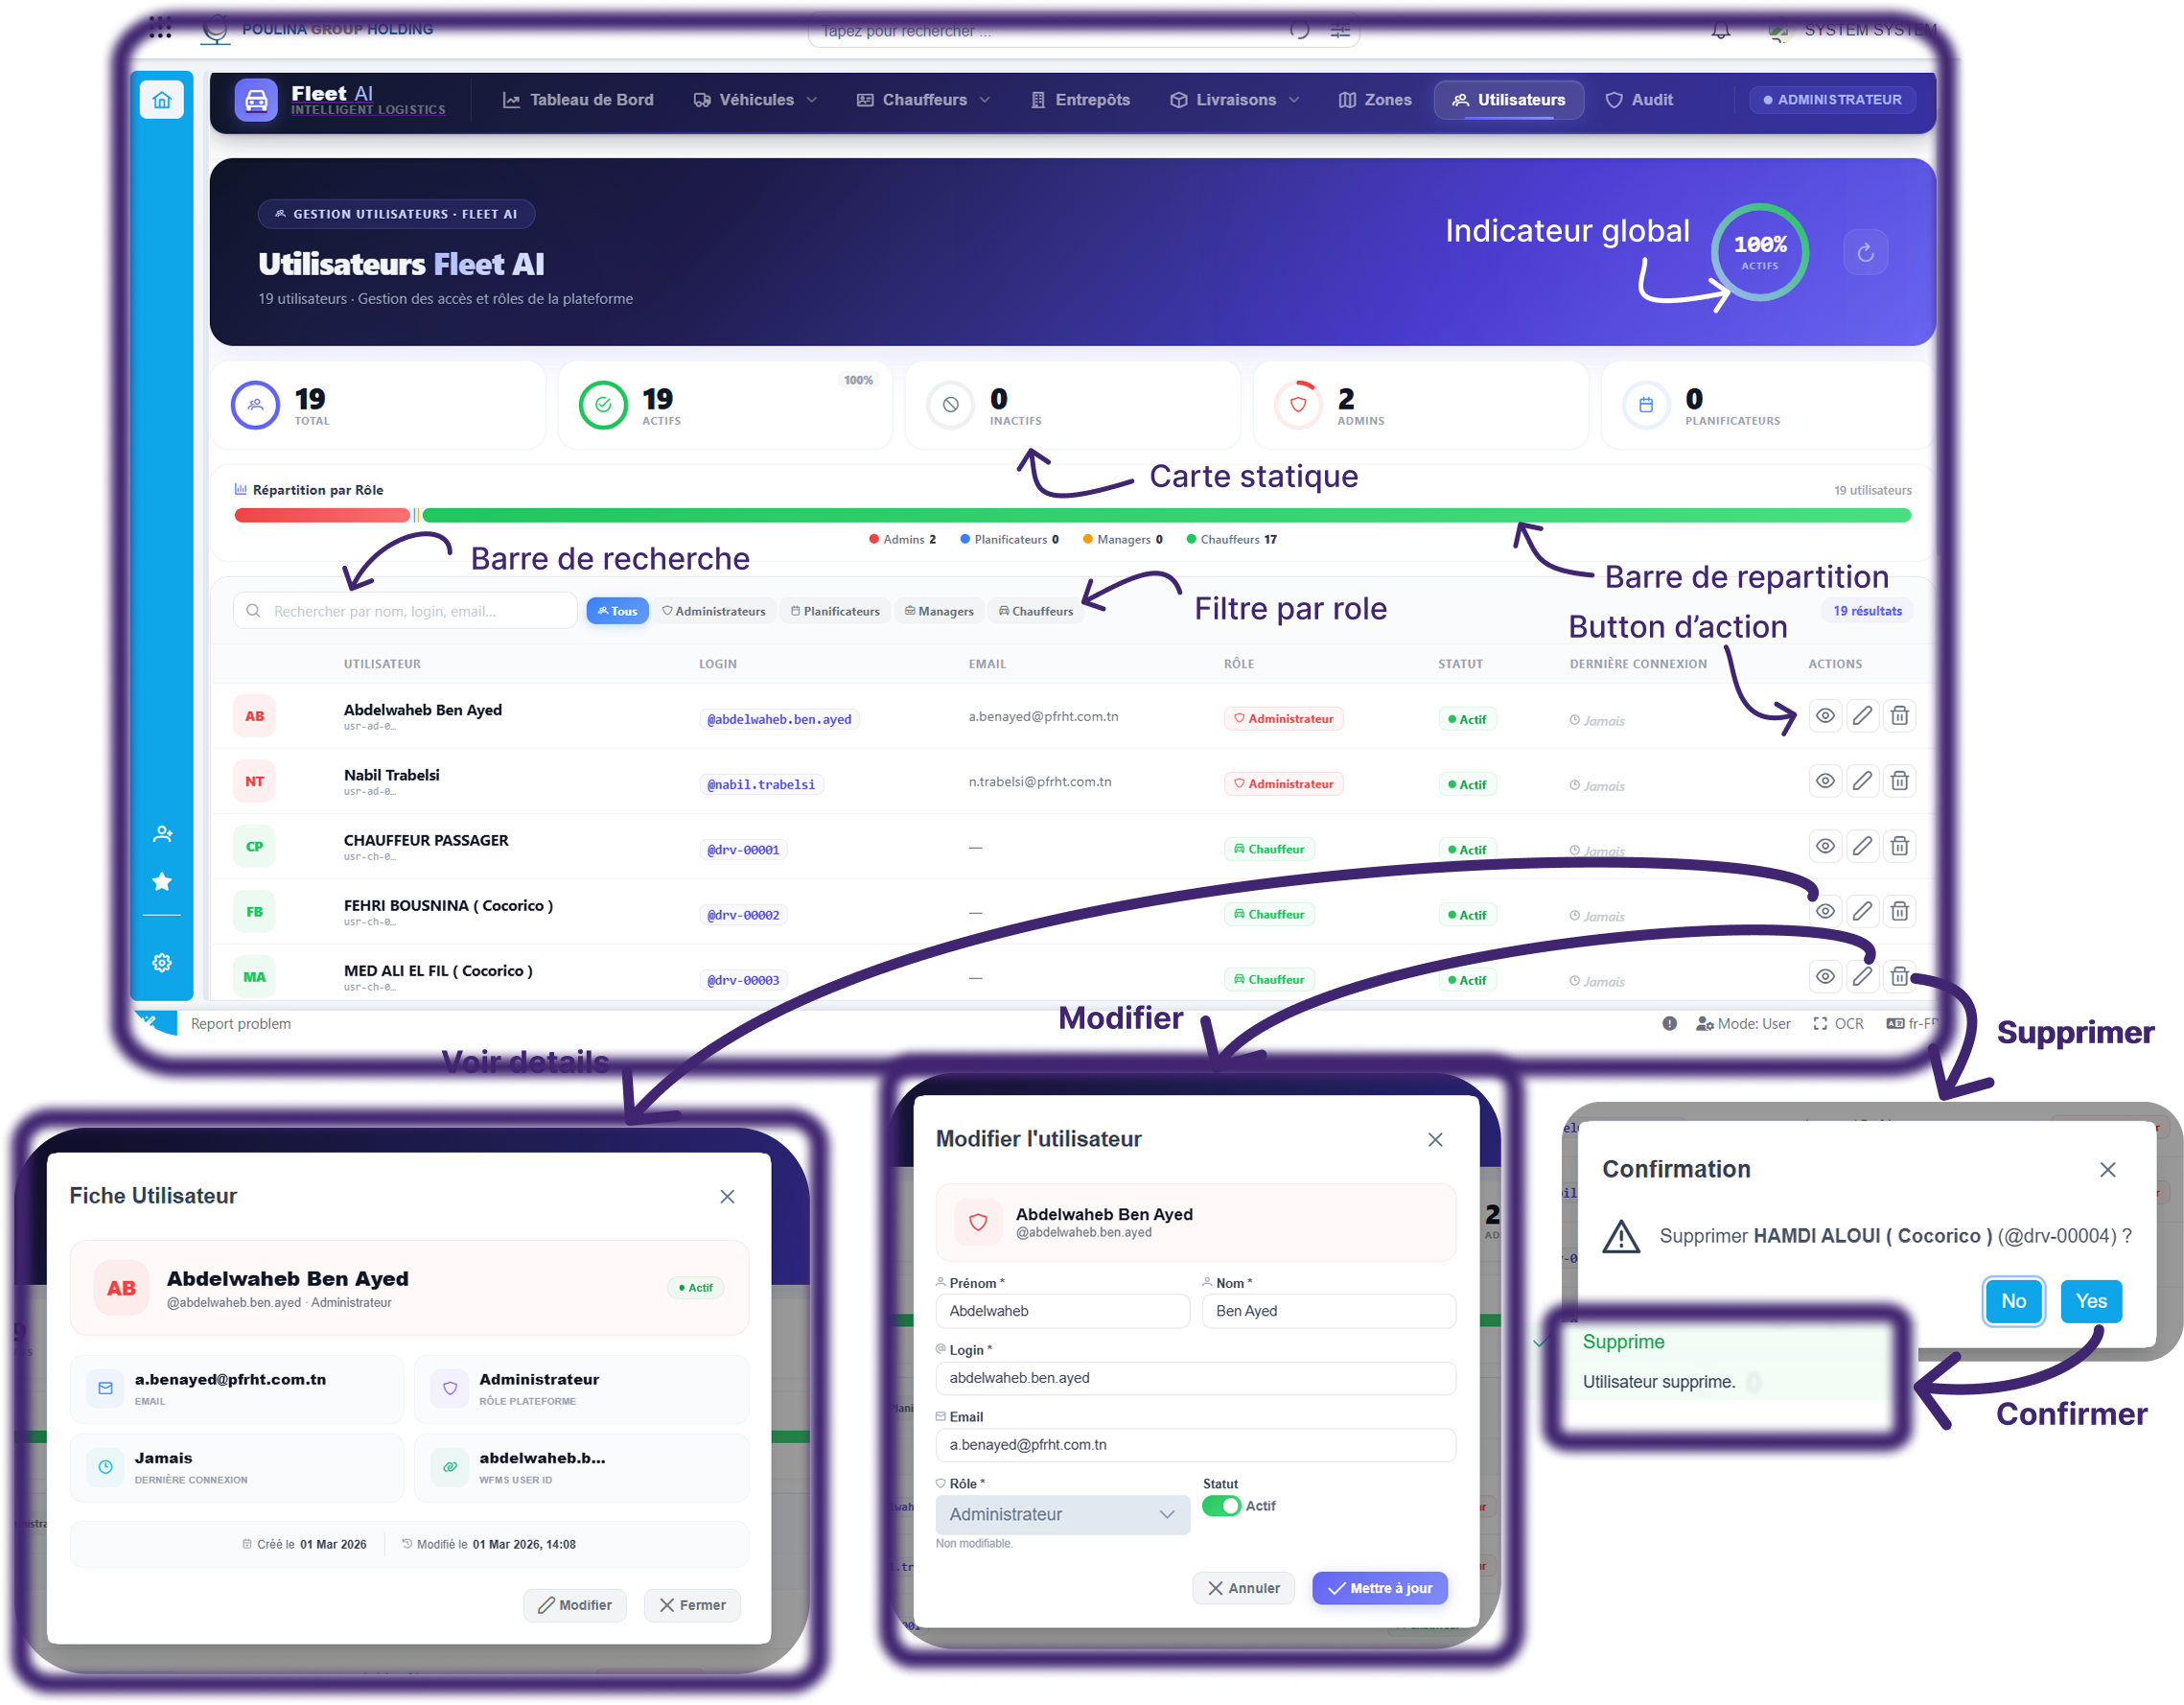
\includegraphics[width=\linewidth, keepaspectratio]{img/capture/web/sp1_users_composite}%
}{%
  \fbox{\parbox{0.9\linewidth}{\centering\vspace{4cm}\textit{[img/sp1\_users\_composite]}\vspace{4cm}}}%
}
\caption{Gestion des utilisateurs : liste par rôle et formulaire de création}
\label{fig:sp1-users}
\end{figure}

\subsection{Gestion des véhicules}

Chaque véhicule est défini par son immatriculation, ses capacités (poids, volume), son statut et sa zone d'affectation. Le suivi des coûts et de l'historique kilométrique est intégré.

\begin{figure}[H]
\centering
\IfFileExists{img/capture/web/sp1_vehicles_composite.png}{%
  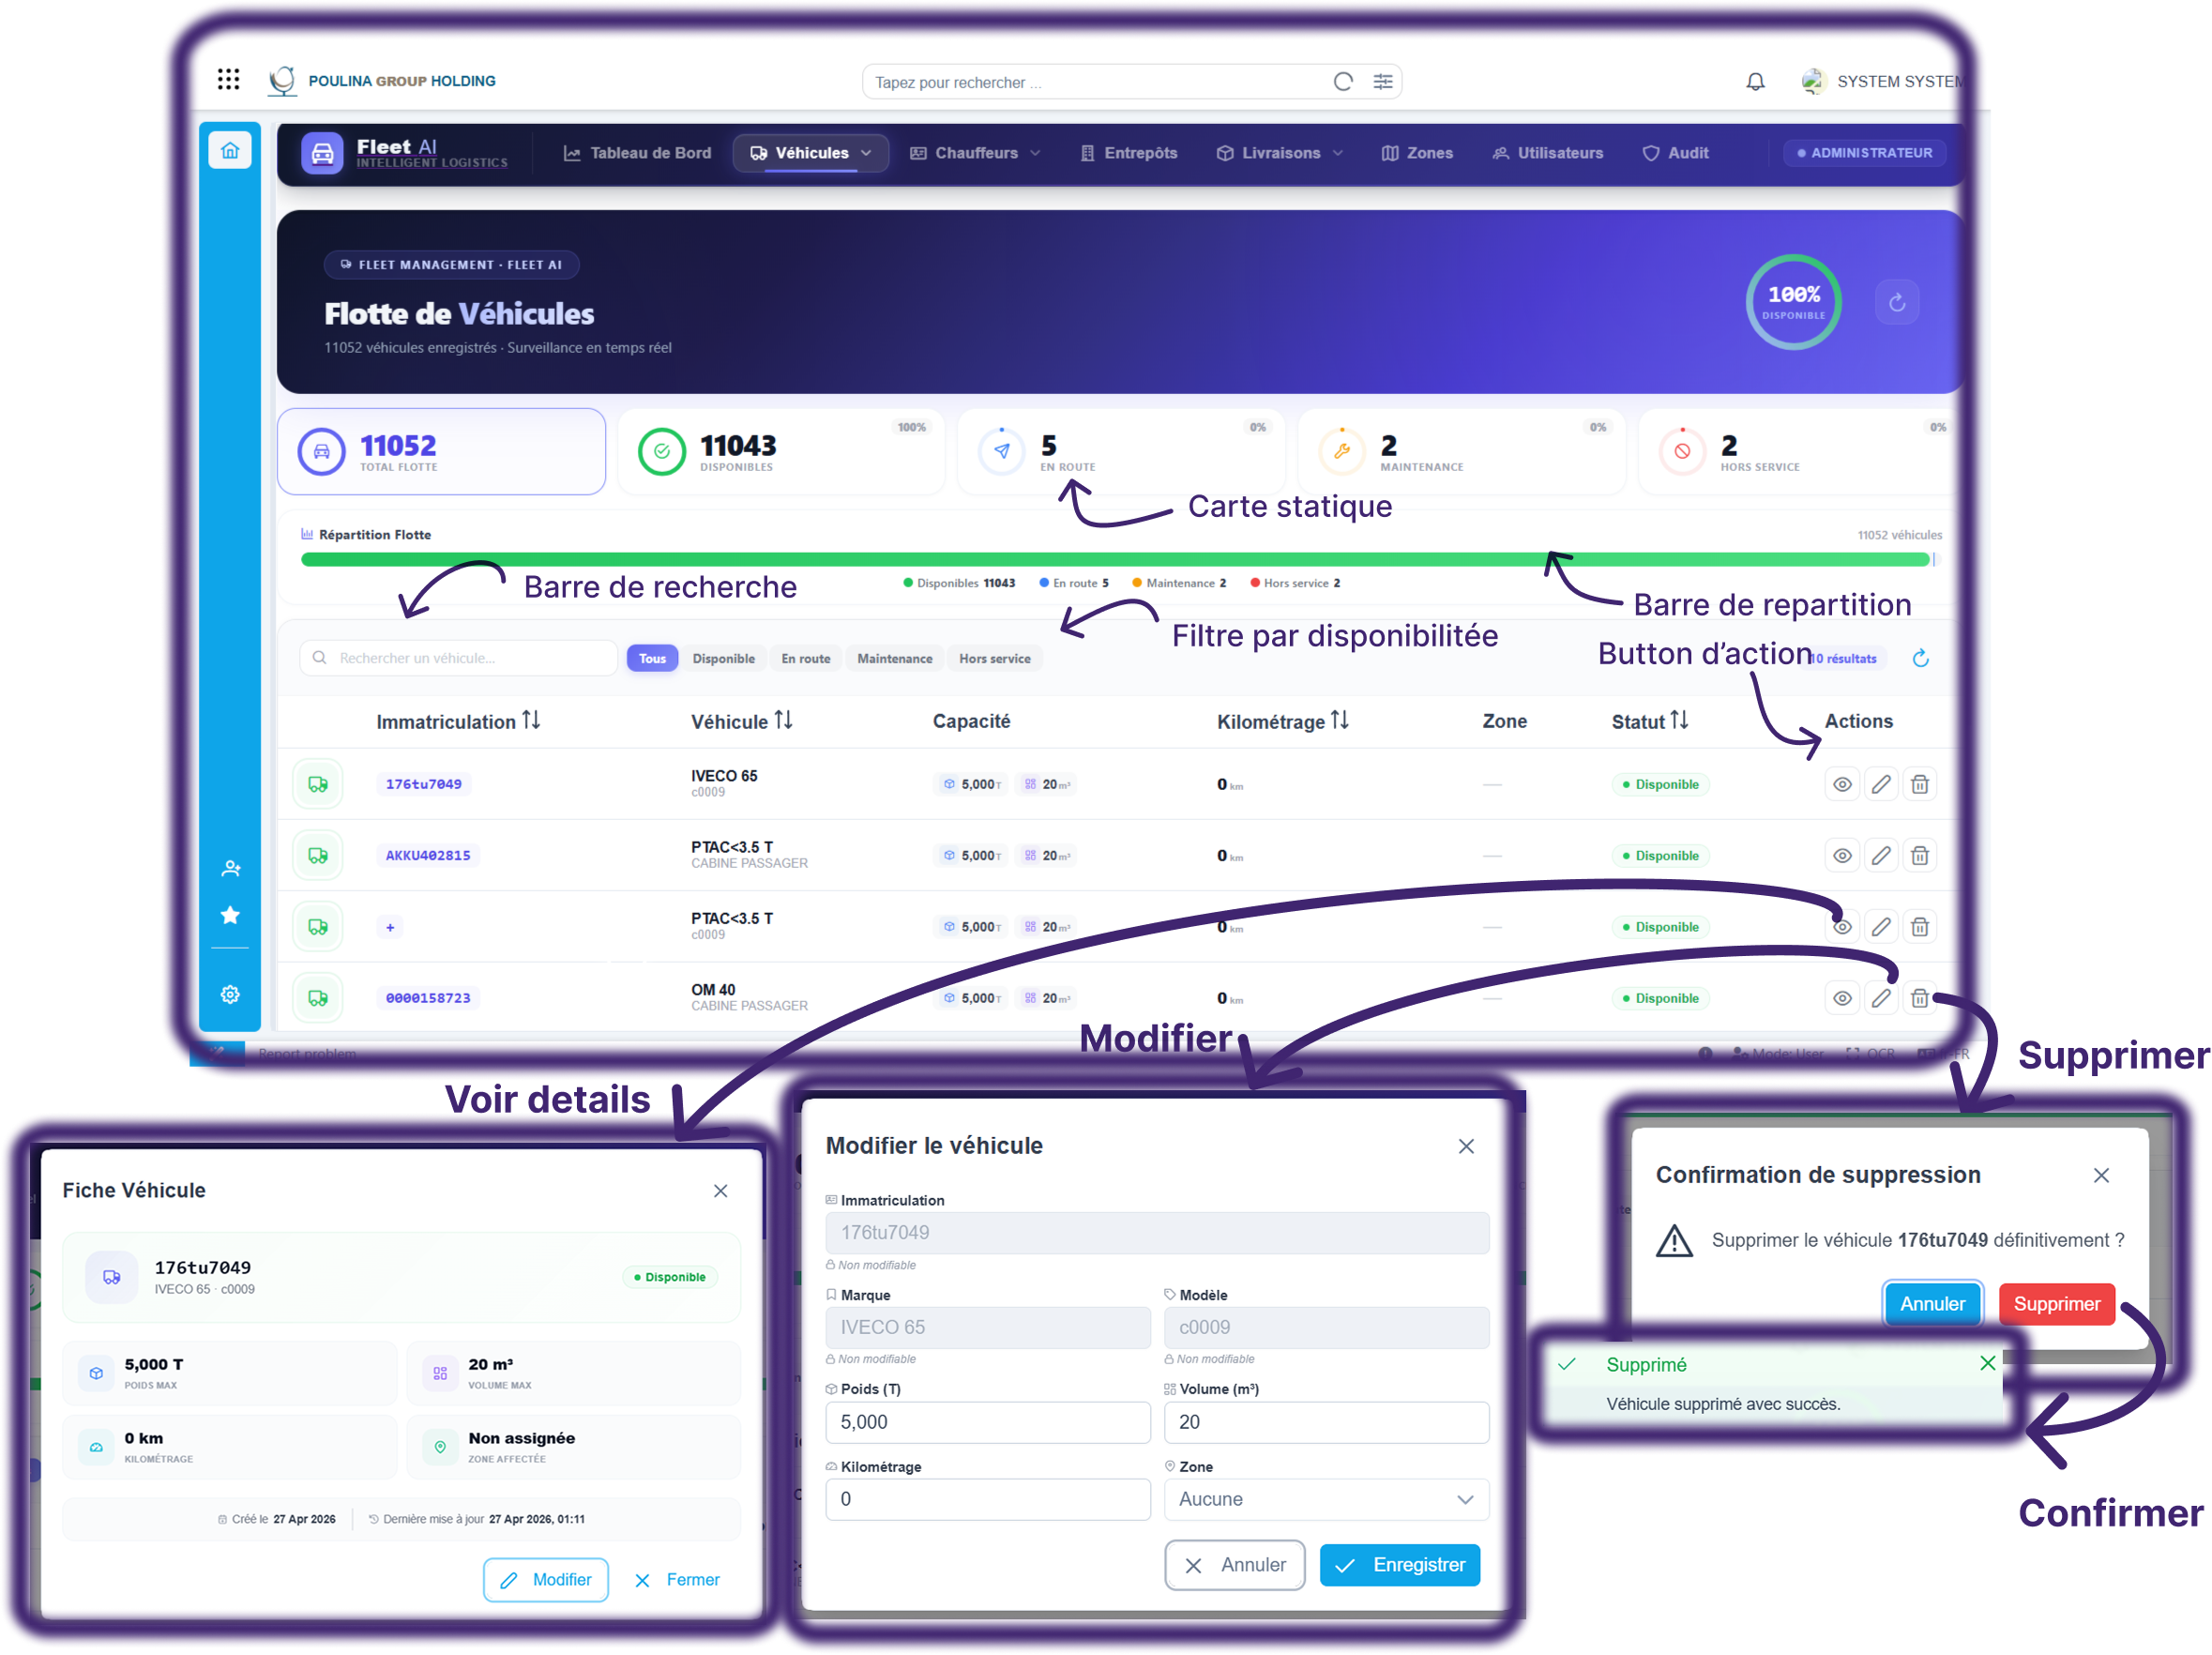
\includegraphics[width=\linewidth, keepaspectratio]{img/capture/web/sp1_vehicles_composite}%
}{%
  \fbox{\parbox{0.9\linewidth}{\centering\vspace{4cm}\textit{[img/sp1\_vehicles\_composite]}\vspace{4cm}}}%
}
\caption{Gestion des véhicules : statuts, capacités et formulaire d'ajout}
\label{fig:sp1-vehicles}
\end{figure}

\subsection{Gestion des chauffeurs}

Le cycle de vie complet est couvert : création avec type de permis (B, C, CE, D, DE), zone d'affectation et contrat (Officiel / Prestataire). Le score global est calculé automatiquement à partir de trois coefficients configurables.

\begin{figure}[H]
\centering
\IfFileExists{img/capture/web/sp1_drivers_composite.png}{%
  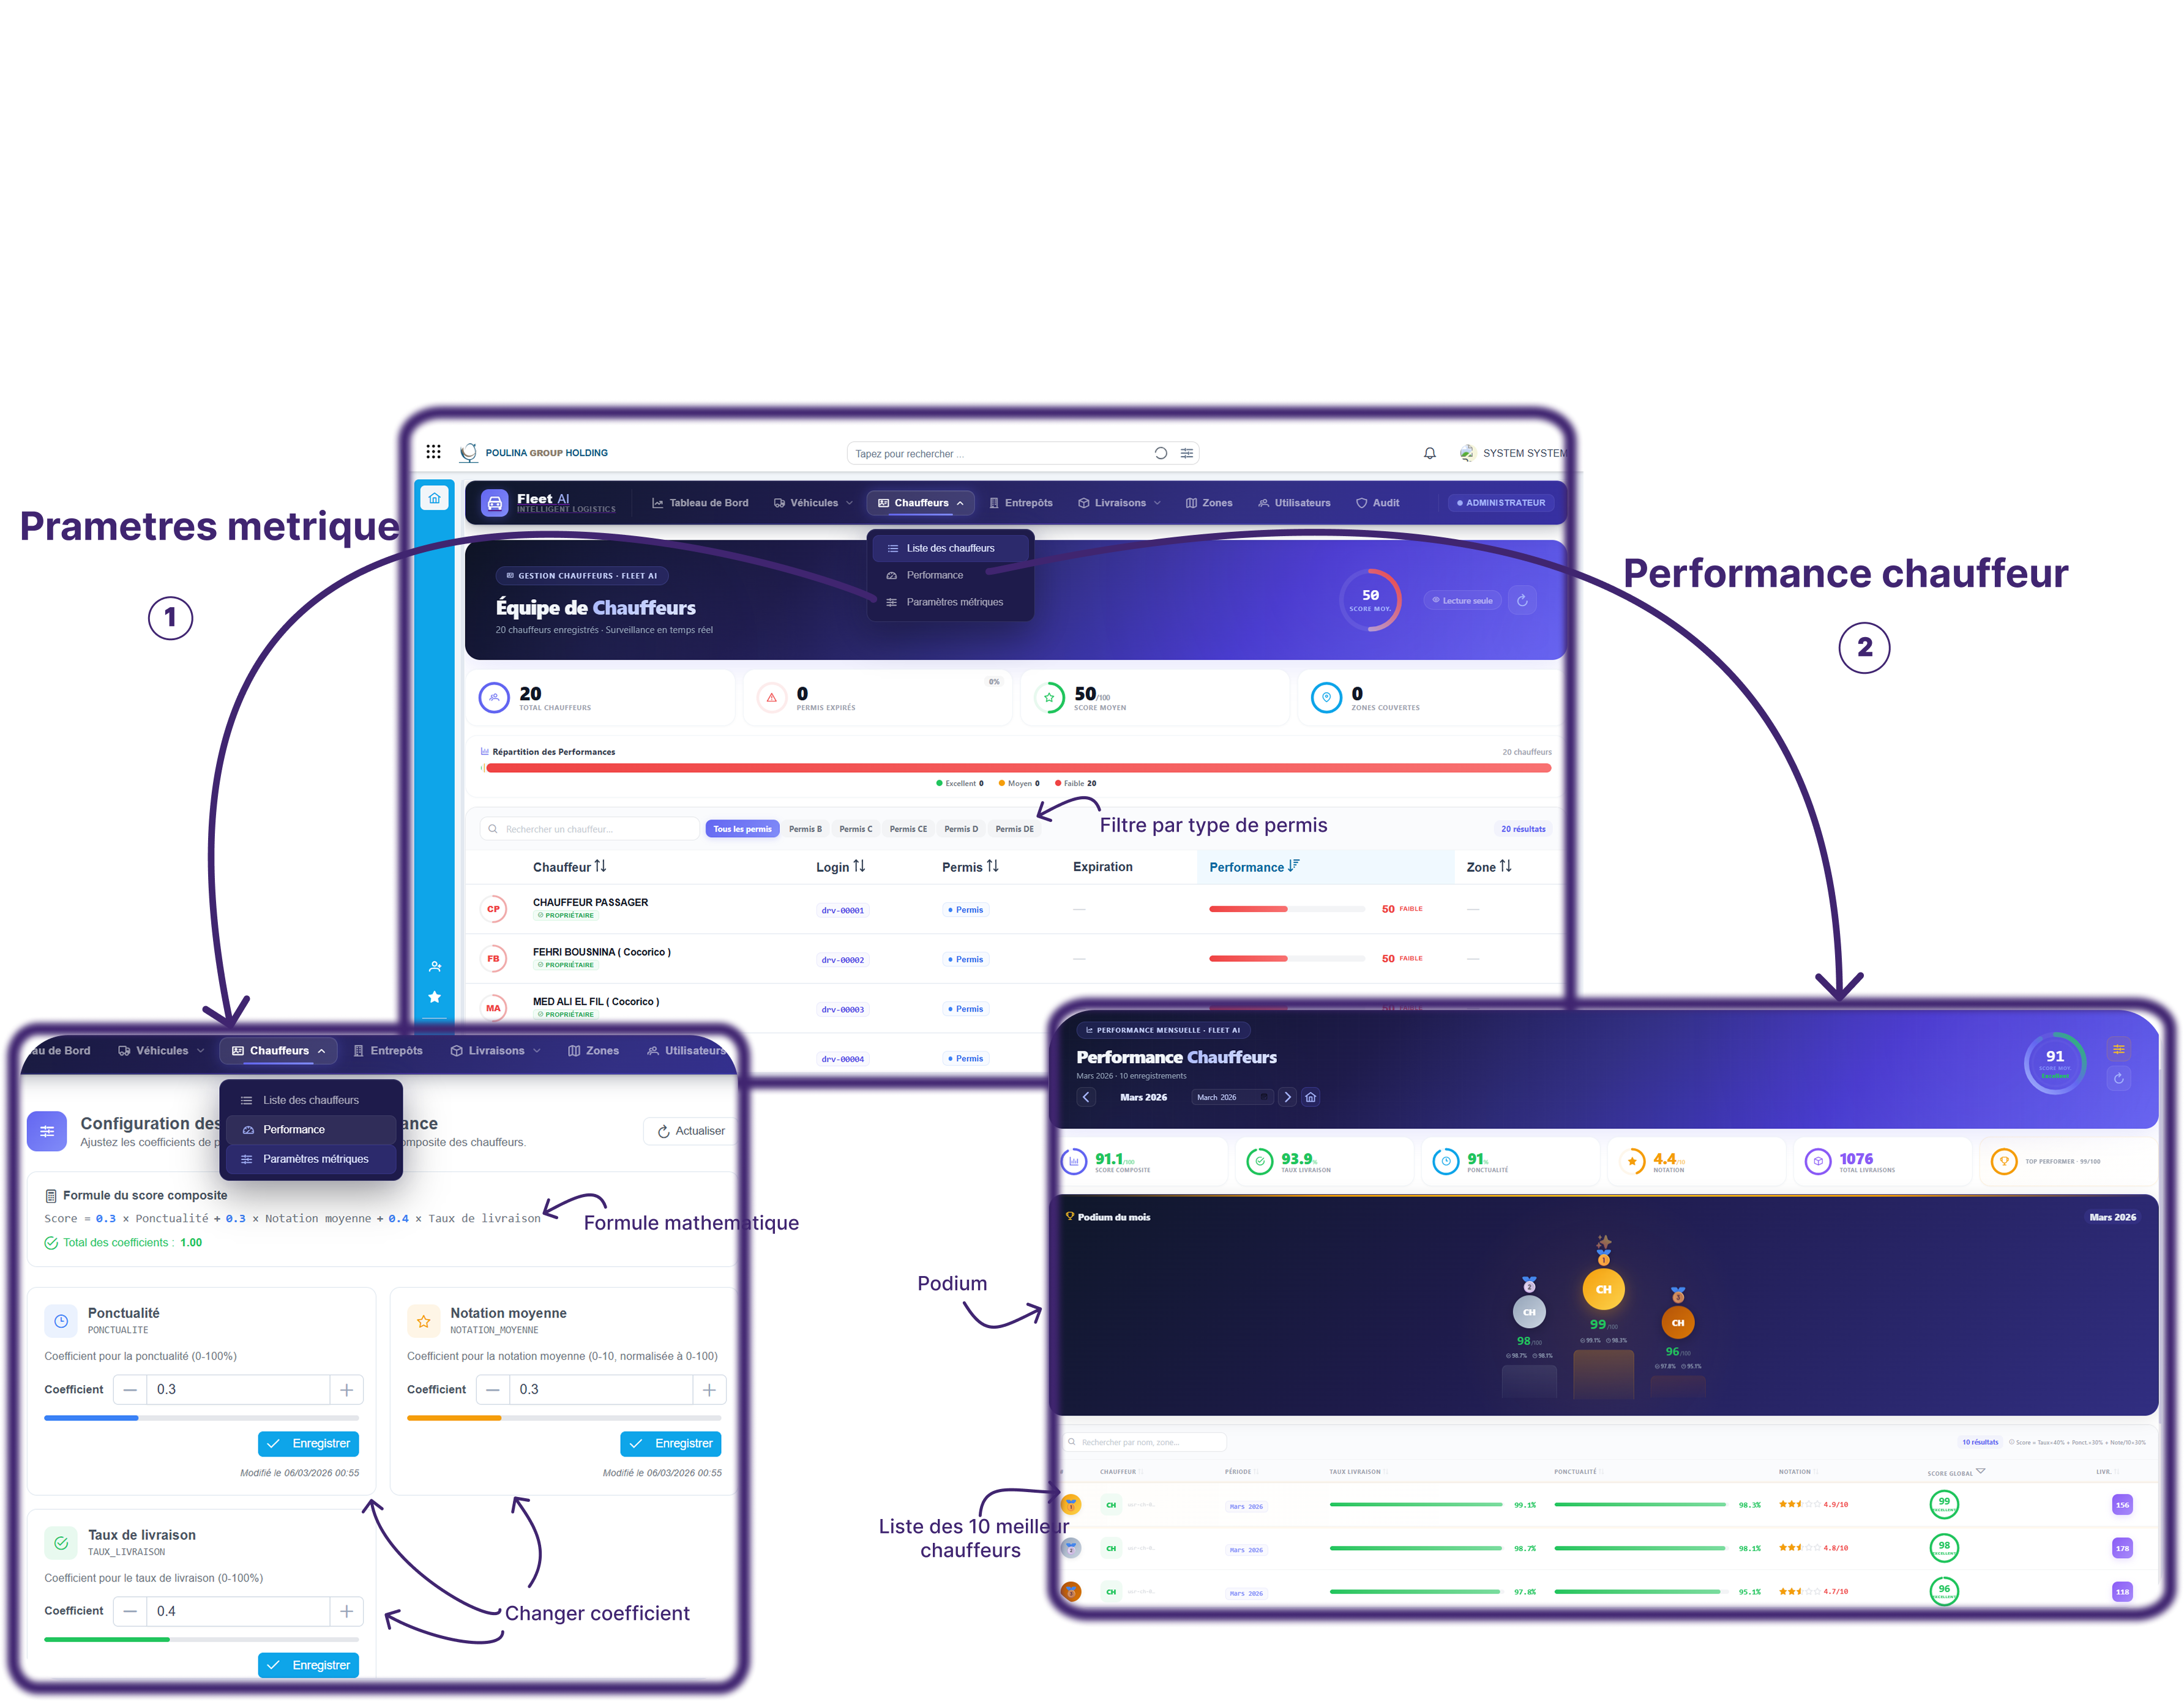
\includegraphics[width=\linewidth, keepaspectratio]{img/capture/web/sp1_drivers_composite}%
}{%
  \fbox{\parbox{0.9\linewidth}{\centering\vspace{4cm}\textit{[img/sp1\_drivers\_composite]}\vspace{4cm}}}%
}
\caption{Gestion des chauffeurs : score, performance et type de permis}
\label{fig:sp1-drivers}
\end{figure}

\subsection{Gestion des zones géographiques}

La gestion des zones permet de définir les périmètres de livraison. Deux types de zones sont supportés : \texttt{STATE\_BASED} (24 gouvernorats tunisiens) et \texttt{MANUAL\_POLYGON} (zones dessinées librement sur carte Leaflet). La détection automatique de zone s'effectue lors de l'ajout d'une adresse client.

\begin{figure}[H]
\centering
\IfFileExists{img/capture/web/sp1_zones_composite.png}{%
  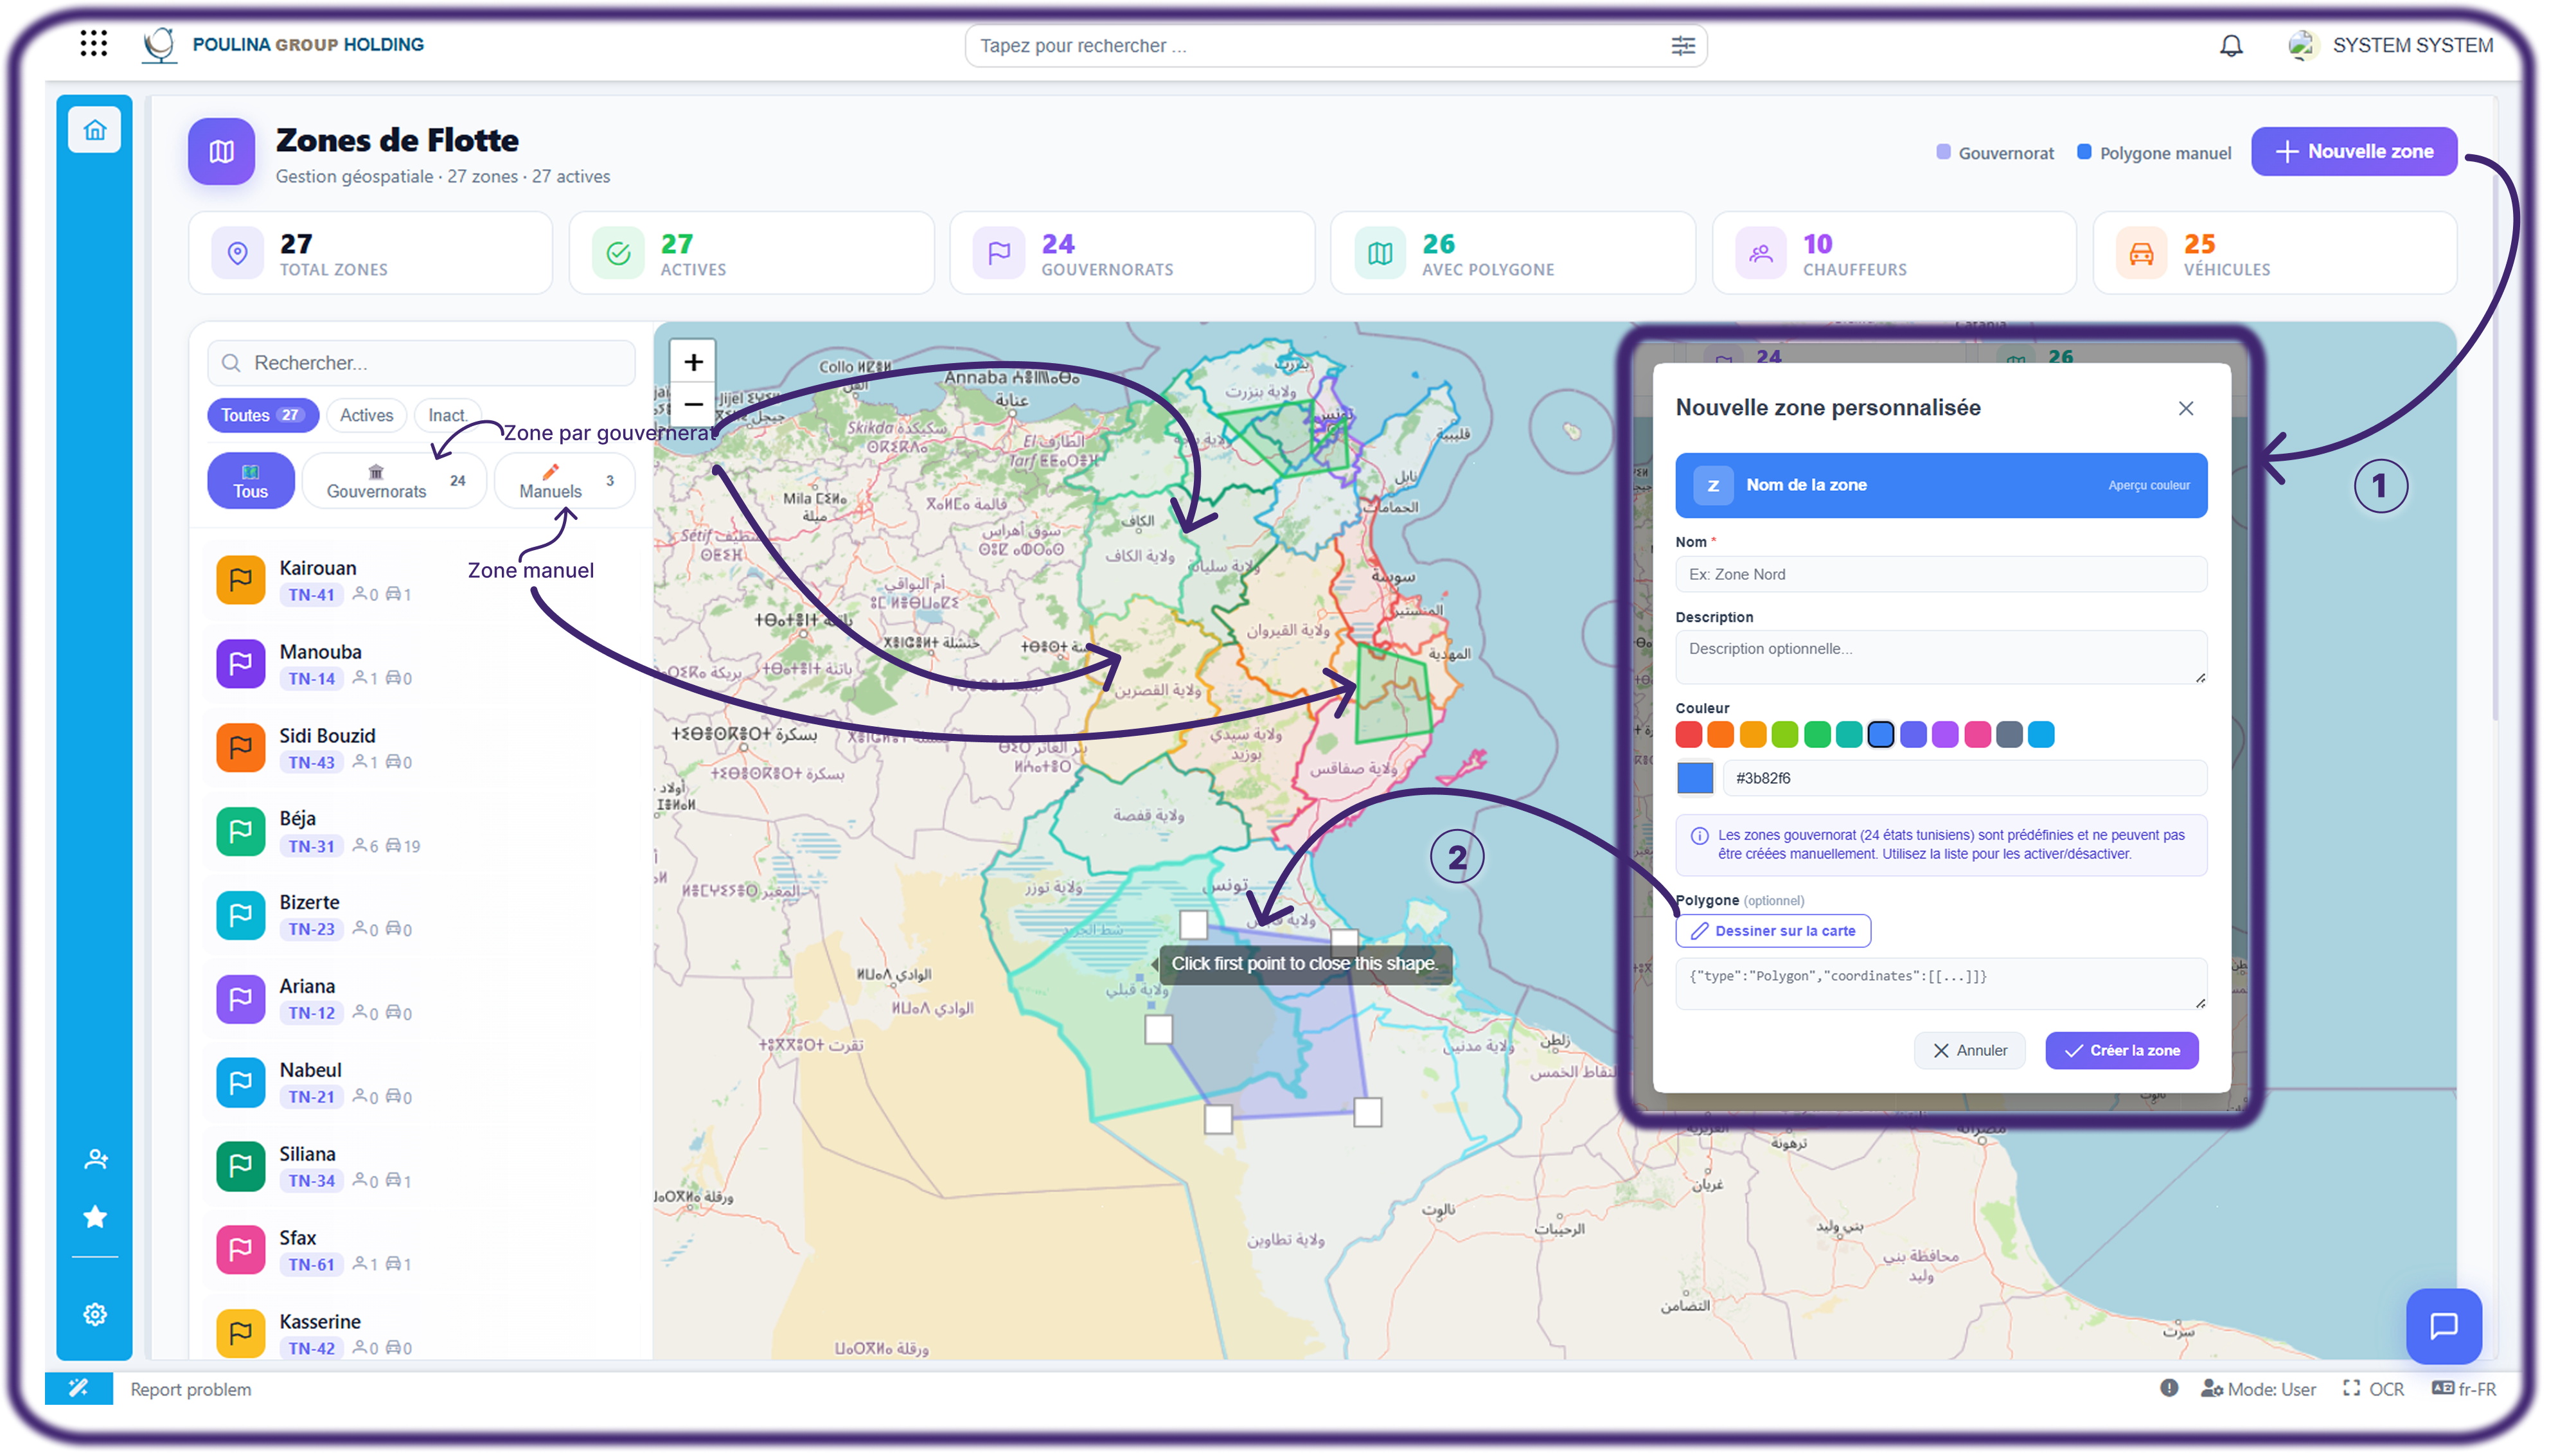
\includegraphics[width=\linewidth, keepaspectratio]{img/capture/web/sp1_zones_composite}%
}{%
  \fbox{\parbox{0.9\linewidth}{\centering\vspace{4cm}\textit{[img/sp1\_zones\_composite]}\vspace{4cm}}}%
}
\caption{Gestion des zones : périmètres et éditeur de polygone Leaflet}
\label{fig:sp1-zones}
\end{figure}

\subsection{Journal d'audit et sauvegardes}

Toutes les actions critiques sont enregistrées automatiquement dans le journal d'audit avec double stockage PostgreSQL et MongoDB. L'Administrateur filtre le journal par date, utilisateur et action. La fonctionnalité de sauvegarde déclenche une copie complète de la base.

\begin{figure}[H]
\centering
\IfFileExists{img/capture/web/sp1_audit_composite.png}{%
  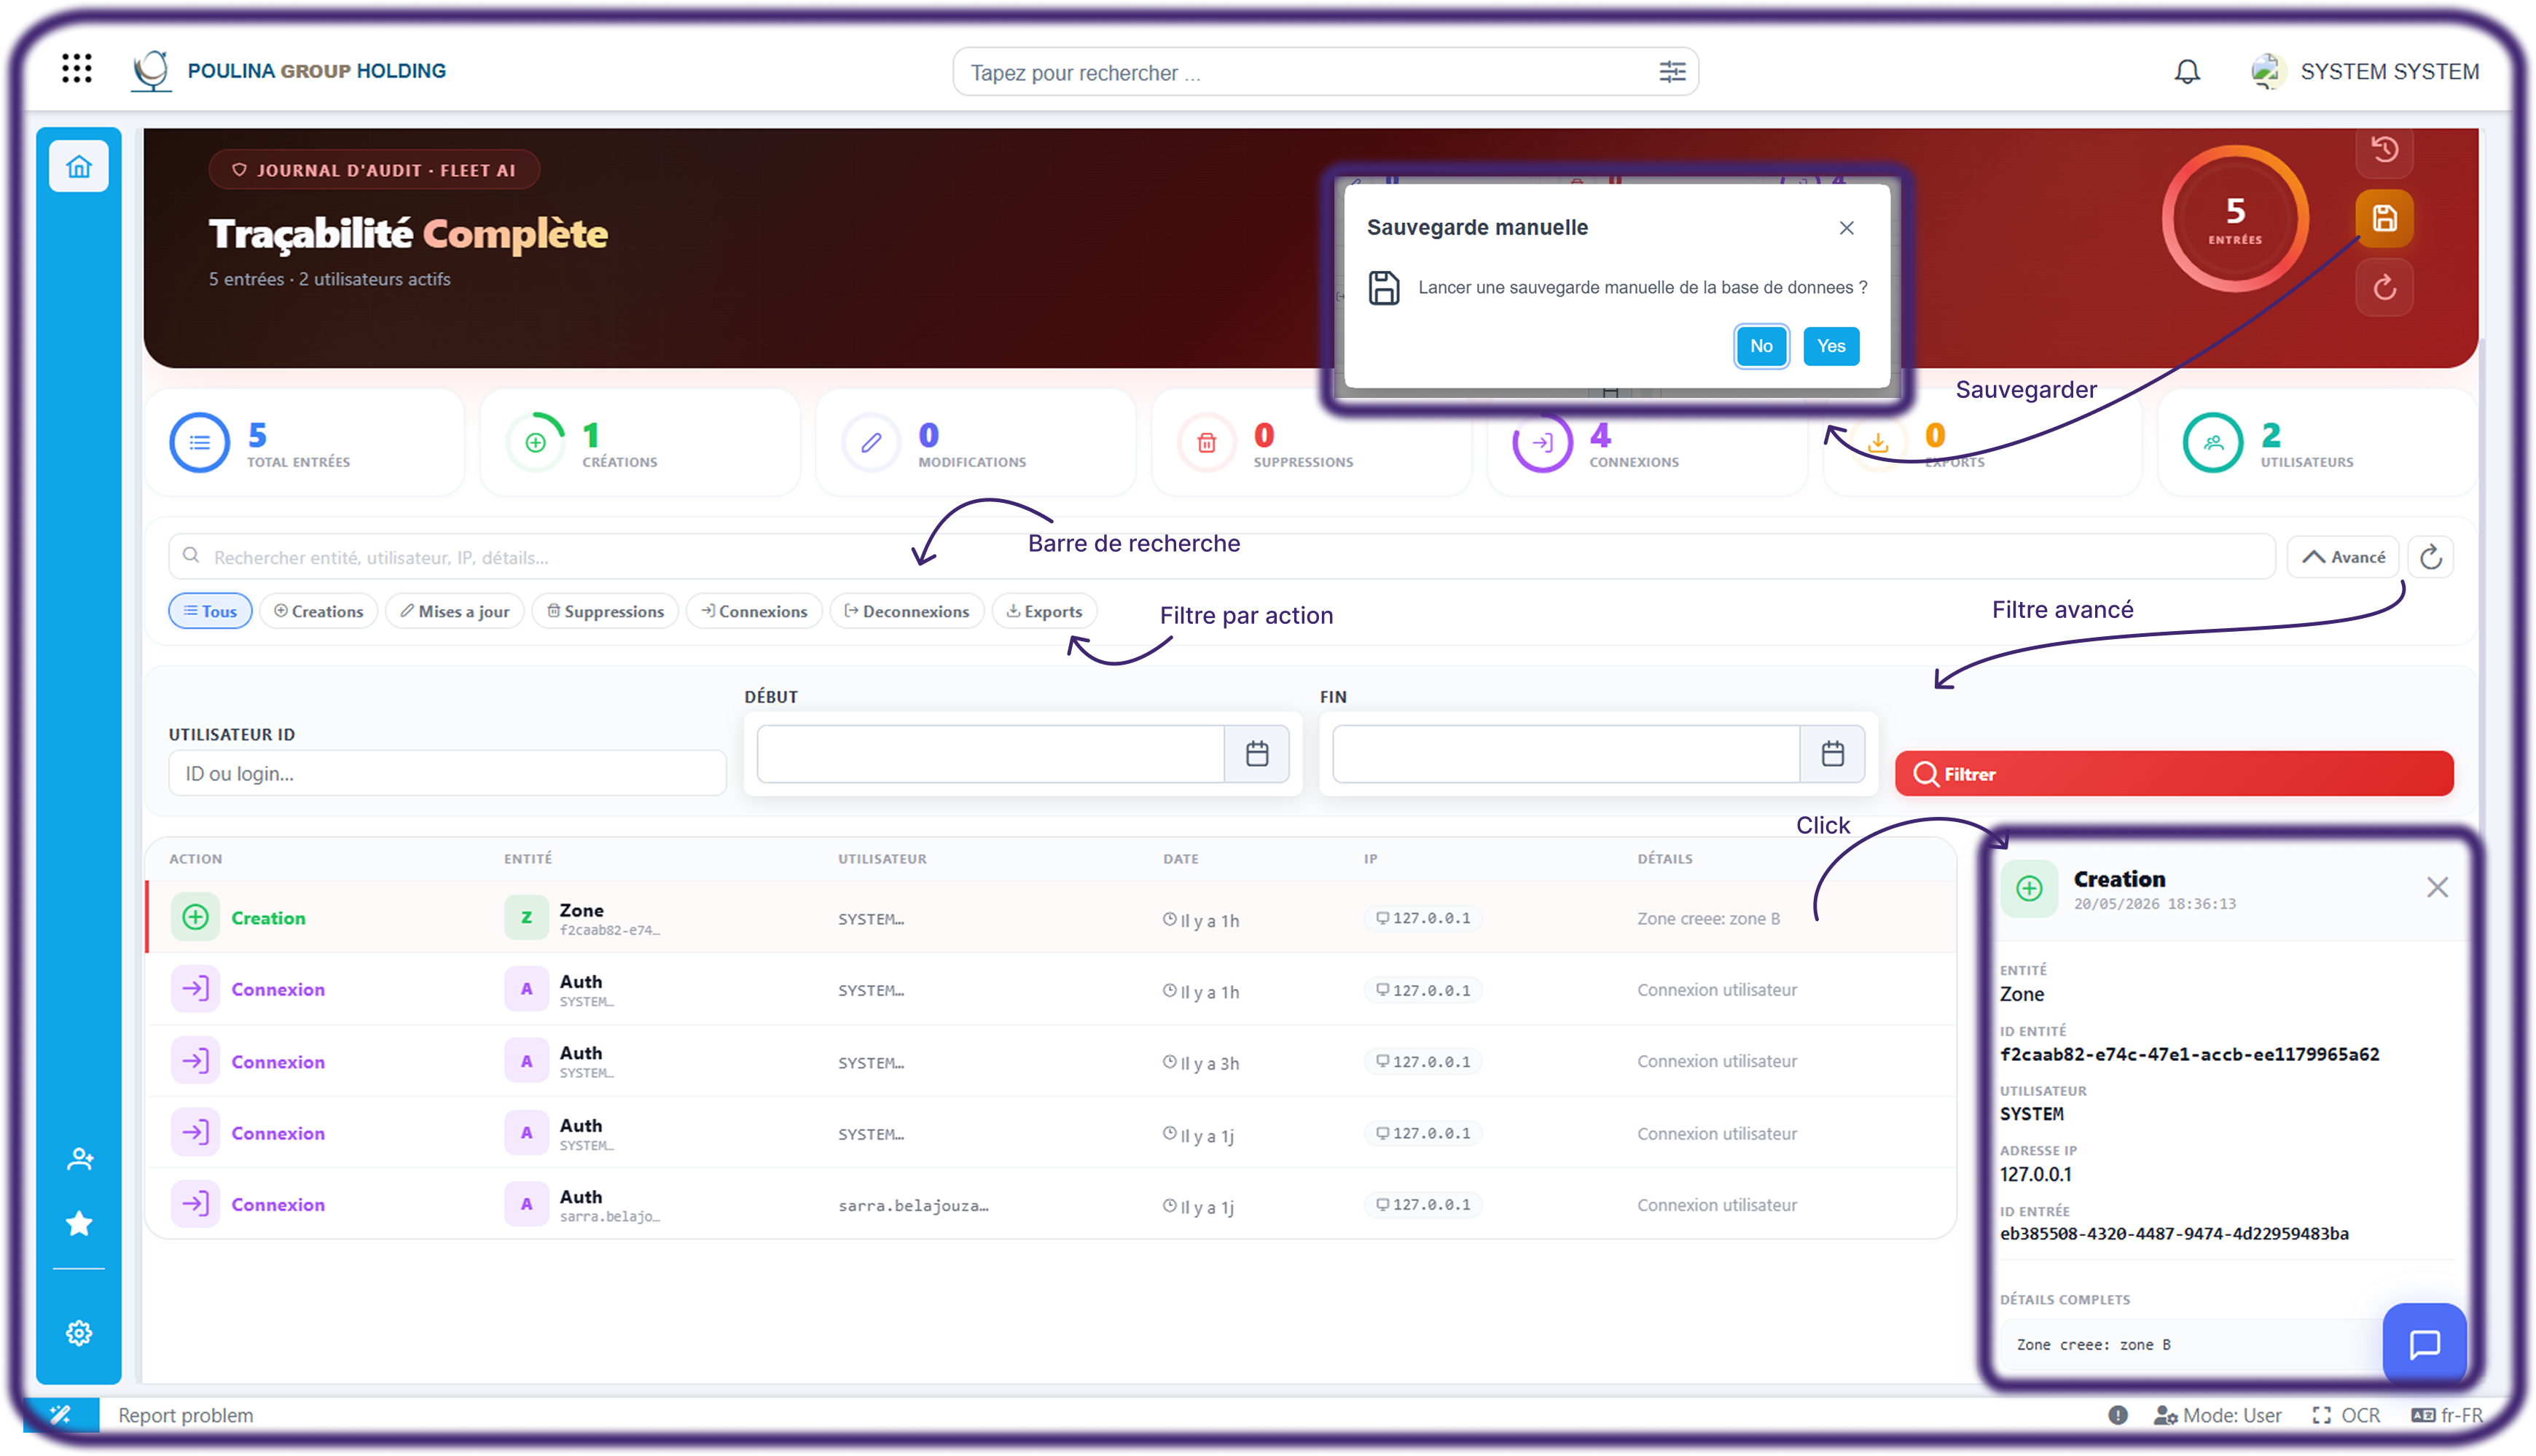
\includegraphics[width=\linewidth, keepaspectratio]{img/capture/web/sp1_audit_composite}%
}{%
  \fbox{\parbox{0.9\linewidth}{\centering\vspace{4cm}\textit{[img/sp1\_audit\_composite]}\vspace{4cm}}}%
}
\caption{Journal d'audit filtrable et déclenchement de sauvegarde}
\label{fig:sp1-audit}
\end{figure}

\subsection{Centre de notifications}

Le système intègre un centre de notifications temps réel (WebSocket). Les utilisateurs configurent leurs préférences (push in-app) par type d'événement.

\begin{figure}[H]
\centering
\IfFileExists{img/capture/web/sp1_notifications_composite.png}{%
  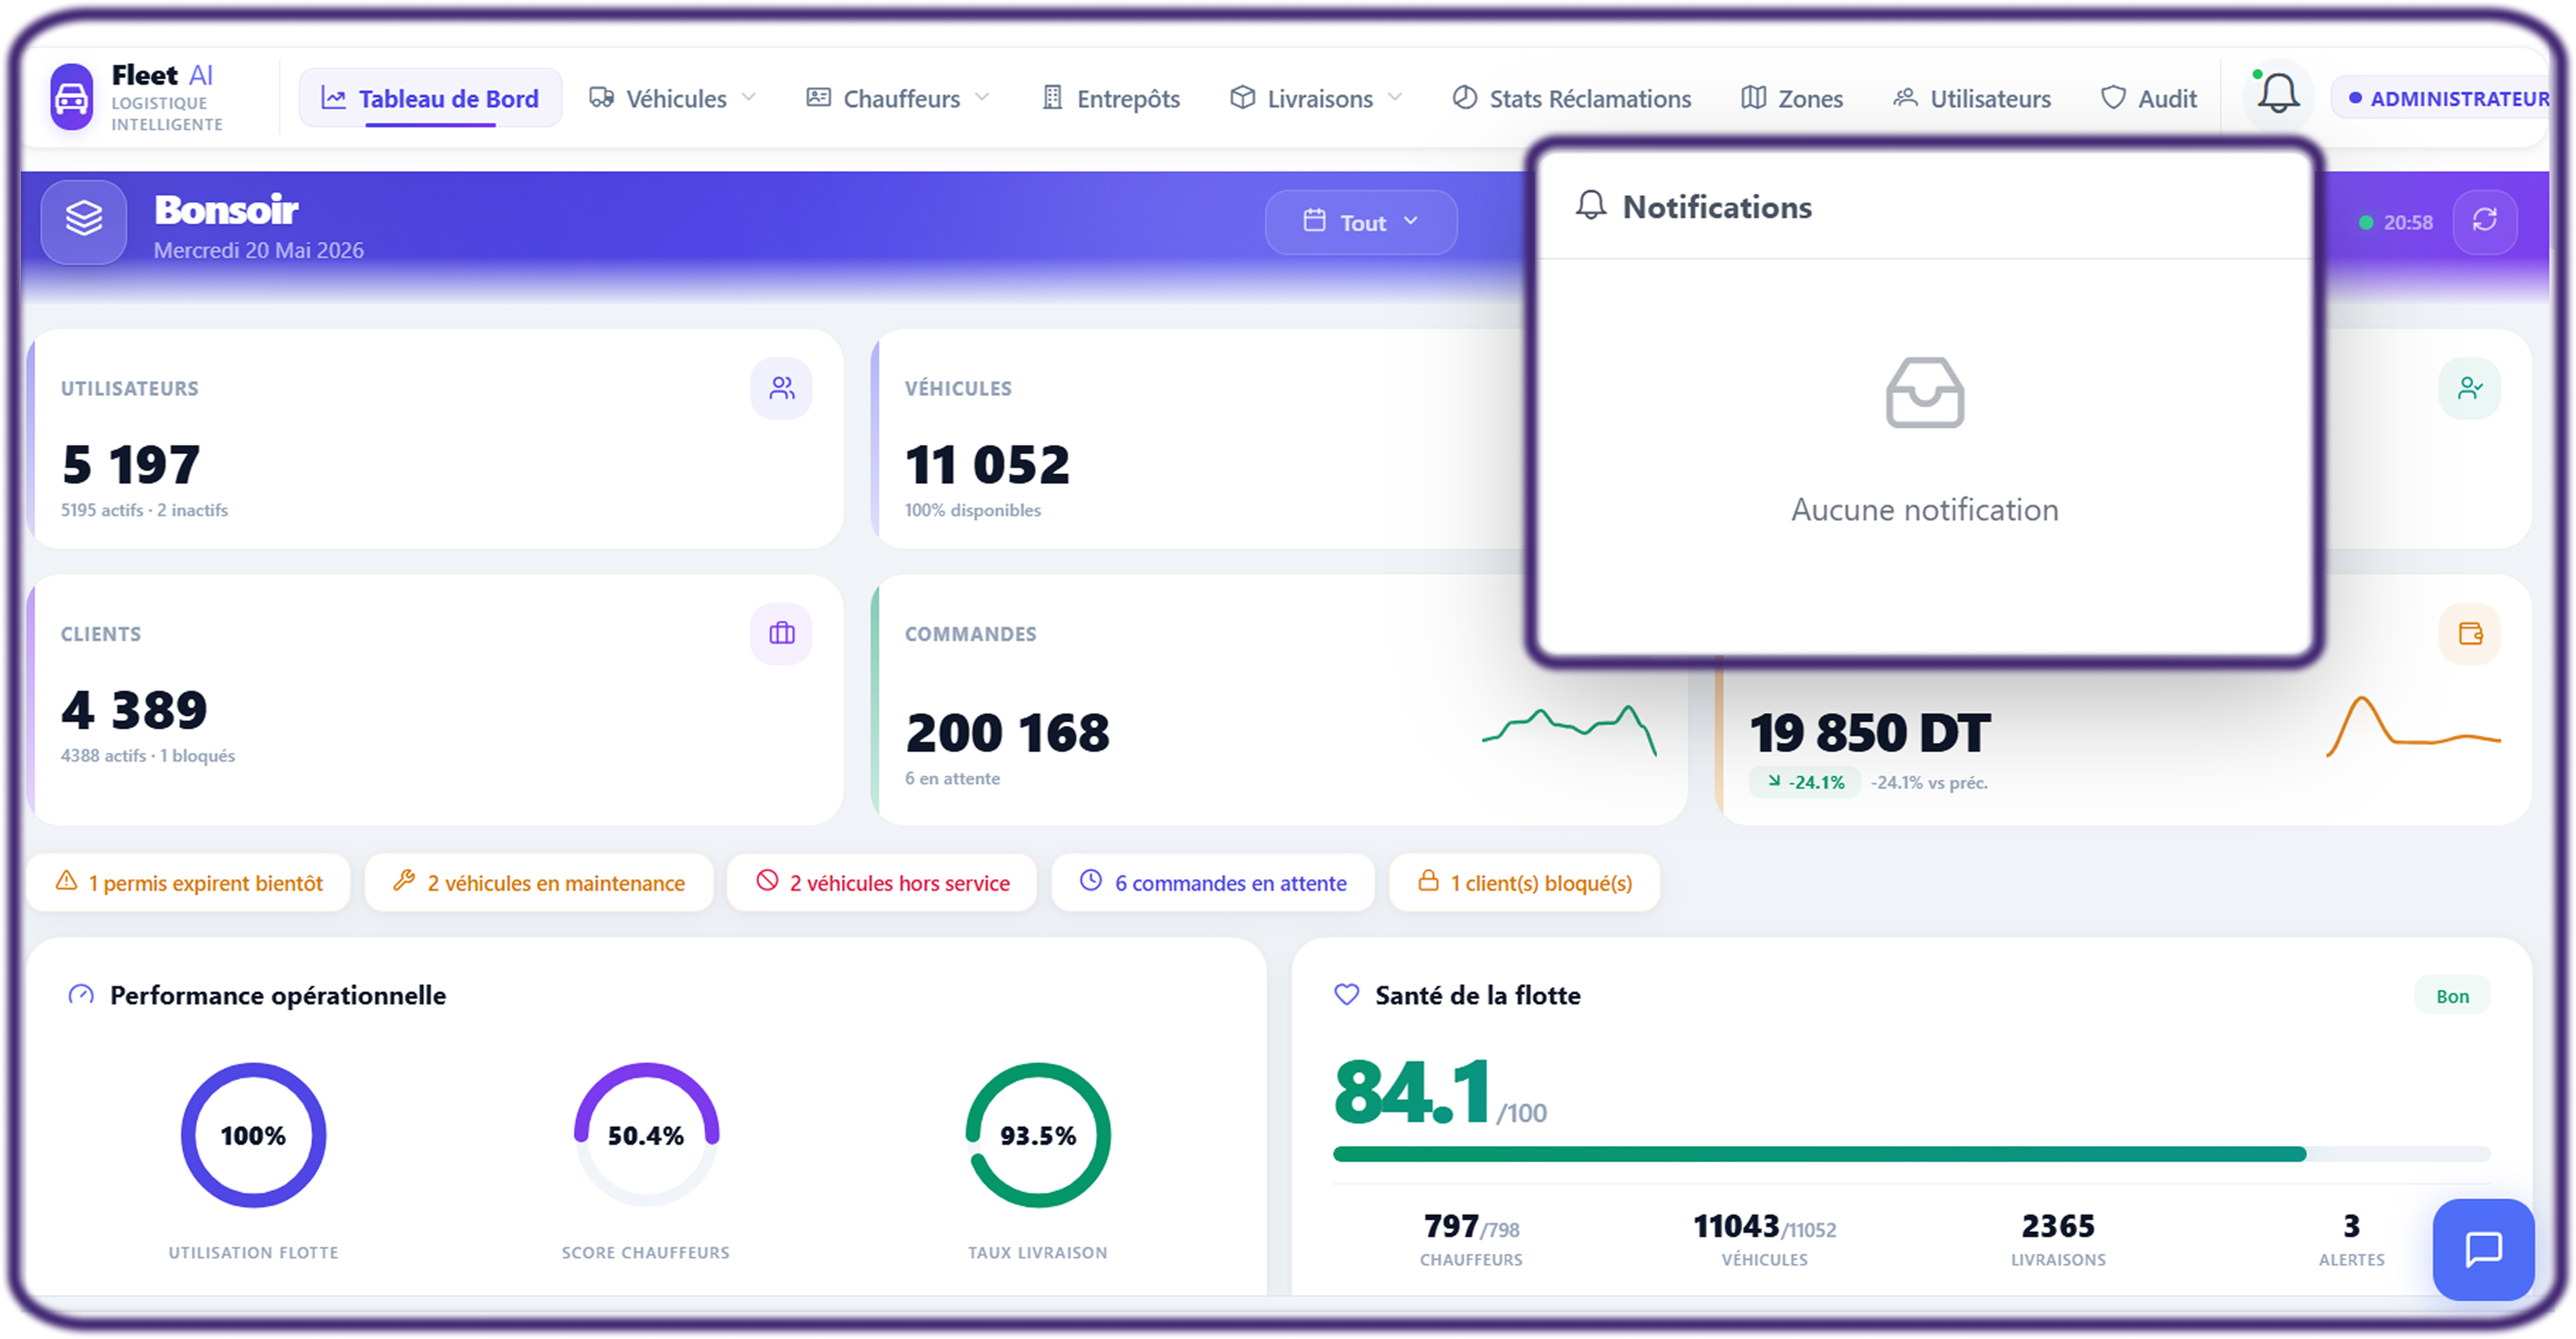
\includegraphics[width=\linewidth, keepaspectratio]{img/capture/web/sp1_notifications_composite}%
}{%
  \fbox{\parbox{0.9\linewidth}{\centering\vspace{4cm}\textit{[img/sp1\_notifications\_composite]}\vspace{4cm}}}%
}
\caption{Centre de notifications WebSocket et préférences}
\label{fig:sp1-notifications}
\end{figure}

% =============================================================
\section{Tests}
% =============================================================

Afin de garantir la fiabilité et la robustesse des fonctionnalités développées dès les fondations du projet, une validation rigoureuse a été mise en place à l'aide de tests unitaires.

\begin{itemize}
    \item \textbf{Les Tests Unitaires :} Ils permettent de valider le comportement précis d'un composant logiciel ou d'une méthode de manière totalement isolée, indépendamment du reste du système.
\end{itemize}

\begin{figure}[H]
\centering
\IfFileExists{img/capture/web/sp1_test_junit.png}{%
  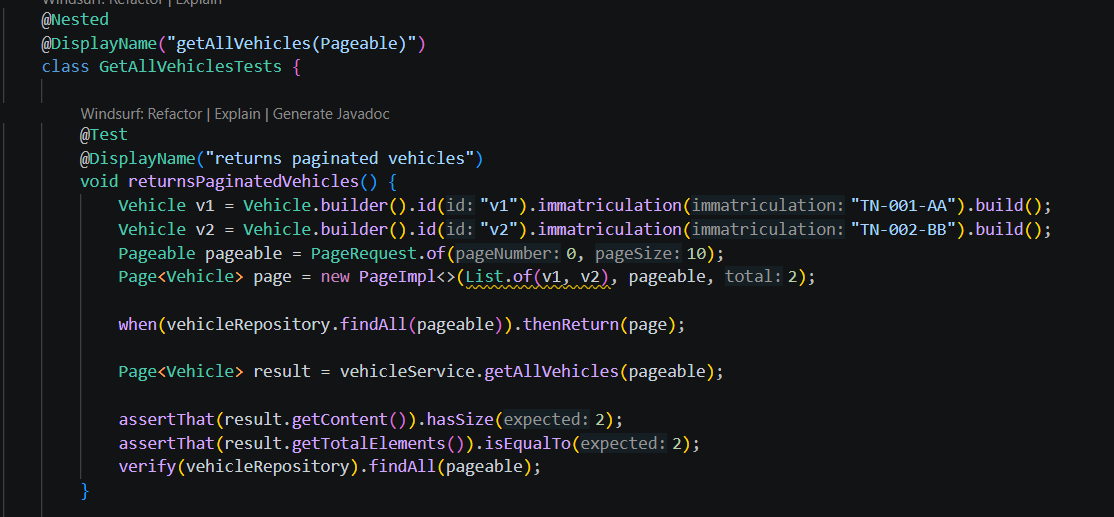
\includegraphics[width=\linewidth, keepaspectratio]{img/capture/web/sp1_test_junit}%
}{%
  \fbox{\parbox{0.9\linewidth}{\centering\vspace{4cm}\textit{[img/capture/web/sp1\_test\_junit.png]}\vspace{4cm}}}%
}
\caption{Exemple d'un test unitaire et résultat d'exécution (Succès)}
\label{fig:sp1-test}
\end{figure}

\section*{Conclusion}
\addcontentsline{toc}{section}{Conclusion}

Le Sprint~1 livre les fondations de Fleet~AI : authentification unifiée via la passerelle WFMS, contrôle d'accès par rôles, gestion complète des référentiels opérationnels (utilisateurs, véhicules, chauffeurs, zones) et journal d'audit avec double persistance. L'application mobile Flutter permet au Chauffeur de consulter son profil et ses performances. Ces composants constituent la base sur laquelle reposent tous les sprints suivants.


% ---- Chapitre 5 : Sprint 2 ----
\chapter{Sprint 2 : Données Métier, Commandes \& Client Mobile}

\section*{Introduction}
\addcontentsline{toc}{section}{Introduction}
Le Sprint~2 enrichit la plateforme avec les entités métier au cœur de l'activité logistique de PGH. La gestion des clients, du stock et du cycle de vie des commandes est mise en place côté web pour le REC et le Planificateur. Le REC peut créer des commandes, vérifier la disponibilité du stock, bloquer ou débloquer un client et consulter son historique complet. En parallèle, l'application mobile Client est développée, permettant de parcourir le catalogue, passer commande et suivre l'avancement des livraisons en temps réel. Ce sprint constitue le cœur fonctionnel de la plateforme, autour duquel s'articulent les sprints de planification et d'exécution terrain.

\section{Sprint Backlog}

\textbf{Objectif du sprint :} L'objectif est de livrer la gestion complète des données métier : référentiel clients, cycle de vie des commandes avec vérification de stock, et application mobile Client avec catalogue et suivi de commandes.

\definecolor{headerbg}{HTML}{d5f5e3}
\setlength{\arrayrulewidth}{1pt}

Les story points (SP) reflètent la complexité et l'effort de chaque tâche, estimés selon la suite de Fibonacci.

\renewcommand{\arraystretch}{0.92}
\begin{longtable}{|>{\raggedright\arraybackslash}p{4.5cm}|>{\raggedright\arraybackslash}p{5.2cm}|>{\raggedright\arraybackslash}p{4.8cm}|c|}
\hline
\rowcolor{headerbg}
\textbf{User Story} & \textbf{Tâche} & \textbf{Critères d'acceptation} & \textbf{\rotatebox{90}{SP}} \\
\hline
\endfirsthead
\hline
\rowcolor{headerbg}
\textbf{User Story} & \textbf{Tâche} & \textbf{Critères d'acceptation} & \textbf{\rotatebox{90}{SP}} \\
\hline
\endhead
\hline
\endfoot

%------ US-094 ------
\multirow{2}{=}{En tant que Responsable des Engagements Clients (REC), je veux gérer le référentiel clients afin de maintenir une base clients à jour.}
& Permettre au REC de créer, modifier et rechercher des clients avec pagination et filtres par nom et code. & Le CRUD complet fonctionne ; la recherche par nom et code est opérationnelle ; pagination et tri intégrés. & 3 \\
\cline{2-4}
& Mettre à disposition du REC une interface de gestion des clients avec liste et formulaire de création. & La liste des clients s'affiche avec filtres ; le formulaire de création/édition fonctionne. & 2 \\
\hline

%------ US-095 ------
\multirow{2}{=}{En tant que Responsable des Engagements Clients, je veux gérer les adresses de livraison de mes clients afin d'assurer des livraisons précises à chaque emplacement.}
& Permettre au REC d'ajouter, modifier et supprimer les adresses de livraison de ses clients avec localisation géographique automatique. & Ajout, modification, suppression d'adresses ; la zone de livraison est détectée automatiquement selon les coordonnées. & 3 \\
\cline{2-4}
& Permettre la désignation d'une adresse par défaut et la détection des doublons géographiques. & Une adresse peut être marquée par défaut ; les adresses en doublon sont signalées. & 2 \\
\hline

%------ US-096 ------
\multirow{2}{=}{En tant que REC, je veux consulter l'historique complet d'un client afin de piloter la relation client.}
& Rassembler pour le REC l'ensemble des commandes, paiements et réclamations d'un client dans une vue unifiée. & La vue agrège les commandes passées, les paiements effectués et les réclamations ouvertes ; filtrable par période. & 3 \\
\cline{2-4}
& Organiser l'historique client en sections distinctes consultables depuis la fiche client. & Les sections Commandes, Paiements et Réclamations s'affichent avec les données correctes. & 2 \\
\hline

%------ US-097 ------
\multirow{2}{=}{En tant que REC, je veux bloquer un client afin de suspendre ses commandes en cas de litige.}
& Permettre au REC de bloquer un client avec saisie obligatoire du motif et notification automatique au client. & Le blocage est immédiat avec motif obligatoire ; le client est notifié automatiquement. & 2 \\
\cline{2-4}
& Demander une confirmation au REC avant l'action de blocage avec saisie du motif obligatoire. & La confirmation exige un motif non vide avant validation ; le statut est mis à jour dans la liste. & 1 \\
\hline

%------ US-098 ------
\multirow{2}{=}{En tant que REC, je veux débloquer un client précédemment bloqué en conservant l'historique de blocage.}
& Permettre au REC de débloquer un client ; l'historique complet des blocages est conservé et consultable. & Le déblocage réactive le compte client ; l'historique des blocages est conservé et consultable. & 2 \\
\cline{2-4}
& Afficher l'option de déblocage uniquement pour les clients bloqués, avec traçabilité de l'action. & L'option de déblocage est visible uniquement pour les clients bloqués ; l'action est tracée dans le journal. & 1 \\
\hline

%------ US-100 ------
\multirow{2}{=}{En tant que Responsable des Engagements Clients, je veux que la création d'une commande soit refusée pour un client bloqué afin d'éviter toute expédition non autorisée.}
& Vérifier systématiquement le statut de blocage du client avant d'accepter la création d'une commande. & Toute tentative de commande pour un client bloqué est refusée avec un message explicite au REC. & 2 \\
\cline{2-4}
& Afficher un message d'erreur clair au REC lors de la tentative de création de commande pour un client bloqué. & Le message d'erreur est clair ; la soumission du formulaire est bloquée tant que le client reste suspendu. & 1 \\
\hline

%------ US-102 ------
\multirow{2}{=}{En tant que REC, je veux définir un niveau de service par client afin de garantir le respect des engagements contractuels.}
& Permettre au REC de définir et mettre à jour le niveau de service (standard, express, premium) par client, avec alerte si le délai est dépassé. & Les niveaux de service sont enregistrés par client ; une alerte est déclenchée si le délai garanti est dépassé. & 2 \\
\cline{2-4}
& Afficher le niveau de service dans la fiche client avec un indicateur visuel coloré. & L'indicateur de niveau de service est visible sur la fiche client et dans la liste. & 1 \\
\hline

%------ US-103 ------
\multirow{2}{=}{En tant que Client, je veux noter le service et le chauffeur après une livraison depuis l'application mobile.}
& Permettre au Client de noter le service et le chauffeur (1 à 5 étoiles) après chaque livraison, avec commentaire optionnel. & Le Client peut noter le service après chaque livraison ; un seul avis est possible par livraison. & 2 \\
\cline{2-4}
& Enregistrer la notation et recalculer la moyenne globale du chauffeur visible par le Manager. & La note est enregistrée et la moyenne recalculée ; visible par le Manager. & 1 \\
\hline

%------ US-007b ------
\multirow{2}{=}{En tant que REC, je veux créer une commande avec vérification de la disponibilité du stock afin d'éviter les ruptures.}
& Vérifier la disponibilité du stock au moment de la création de la commande et refuser si le stock est insuffisant. & La création vérifie le stock disponible ; la commande est refusée si le stock est insuffisant, avec message explicite. & 3 \\
\cline{2-4}
& Afficher au REC la quantité disponible par article lors de la saisie de la commande. & Le formulaire affiche le stock disponible ; la soumission est bloquée si le stock est insuffisant. & 2 \\
\hline

%------ US-008b ------
\multirow{2}{=}{En tant que Planificateur, je veux que le système suive le cycle de vie complet d'une commande afin d'assurer la traçabilité de bout en bout.}
& Implémenter la gestion des transitions d'état de la commande selon un enchaînement strict (créée, acceptée, envoyée, prête, affectée, en cours, livrée ou échouée). & Les transitions sont validées dans l'ordre prévu ; chaque changement est tracé avec l'acteur et la date. & 5 \\
\cline{2-4}
& Afficher visuellement l'avancement de la commande étape par étape dans l'interface du Planificateur. & Chaque changement de statut est visible ; des notifications sont envoyées aux parties prenantes concernées. & 3 \\
\hline

%------ US-009b ------
\multirow{2}{=}{En tant que Client, je veux consulter le statut de mes commandes afin de suivre mes livraisons.}
& Permettre au Client de consulter l'état actuel de chaque commande depuis l'application mobile. & Le Client voit le statut actuel de chaque commande ; l'affichage est mis à jour en temps réel. & 3 \\
\cline{2-4}
& Afficher au Client l'historique des changements de statut de sa commande sous forme de chronologie. & L'historique des transitions de statut est visible sous forme de chronologie. & 2 \\
\hline

%------ US-010b ------
\multirow{2}{=}{En tant que Client, je veux annuler une commande avant son expédition depuis l'application mobile.}
& Permettre au Client d'annuler une commande uniquement si elle n'a pas encore été expédiée ou affectée. & Le Client peut annuler ; l'annulation est refusée si la commande est déjà affectée ou expédiée. & 2 \\
\cline{2-4}
& Afficher le bouton d'annulation uniquement si le statut de la commande le permet, avec confirmation obligatoire. & Le bouton est visible uniquement si le statut autorise l'annulation ; confirmation requise. & 1 \\
\hline

%------ US-011b ------
\multirow{2}{=}{En tant que Planificateur, je veux voir les commandes en attente d'affectation triées par priorité afin d'organiser le traitement.}
& Mettre à disposition du Planificateur la liste des commandes prêtes à être affectées, triées par priorité et par date. & La liste des commandes en attente est accessible au Planificateur ; tri par priorité et par date. & 2 \\
\cline{2-4}
& Permettre au Planificateur de filtrer les commandes en attente par plusieurs critères. & Les filtres multiples fonctionnent ; les résultats sont paginés. & 1 \\
\hline

%------ US-012b ------
\multirow{2}{=}{En tant que REC, je veux consulter le stock réel disponible afin de gérer les commandes en conséquence.}
& Permettre au REC de consulter le niveau de stock réel de chaque article en temps réel. & Le stock réel est consultable ; distinction claire entre stock réel et stock publié. & 2 \\
\cline{2-4}
& Afficher au REC un indicateur de disponibilité par article avec mise à jour en temps réel. & L'affichage distingue le stock réel et le stock publié ; l'indicateur est actualisé en continu. & 1 \\
\hline

%------ US-013b ------
\multirow{2}{=}{En tant que Client, je veux consulter le stock disponible afin de passer commande en connaissance de cause.}
& Permettre au Client de consulter uniquement le stock publié par le REC, sans accès au stock réel. & Le Client voit uniquement le stock publié défini par le REC ; le stock réel n'est jamais exposé. & 2 \\
\cline{2-4}
& Afficher au Client le catalogue d'articles avec le stock publié par article. & L'affichage du catalogue est clair ; le stock publié est visible par article. & 1 \\
\hline

%------ US-014b ------
\multirow{2}{=}{En tant que REC, je veux définir le stock visible par les clients afin de contrôler les informations publiées.}
& Permettre au REC de définir le stock publié par article, dans la limite du stock réel disponible. & Le REC peut définir le stock publié ; la valeur publiée ne peut pas dépasser le stock réel. & 2 \\
\cline{2-4}
& Mettre à jour immédiatement le stock visible par les clients après publication par le REC. & La mise à jour est immédiate ; les clients voient instantanément les nouvelles valeurs publiées. & 1 \\
\hline

%------ US-104 (Affectation REC-Client) ------
\multirow{2}{=}{En tant que Manager, je veux assigner des clients à un Responsable des Engagements Clients afin de structurer les responsabilités commerciales.}
& Permettre au Manager d'affecter et désaffecter des clients à un REC, avec contrainte d'unicité d'affectation. & L'affectation est enregistrée ; un client ne peut être assigné qu'à un seul REC à la fois. & 3 \\
\cline{2-4}
& Permettre au Manager de gérer les affectations en lot depuis une interface dédiée. & L'interface permet d'assigner et désassigner des clients en lot. & 2 \\
\hline

%------ US-109 (Dashboard Manager) ------
\multirow{2}{=}{En tant que Manager, je veux comparer les performances par zone afin d'identifier les zones à améliorer.}
& Calculer les indicateurs de performance agrégés par zone (taux de livraison, délais moyens) et les exposer au Manager. & Les indicateurs sont calculés par zone et disponibles pour la visualisation. & 3 \\
\cline{2-4}
& Afficher au Manager une vue comparative des performances par zone, filtrable par période. & La vue des performances par zone s'affiche avec filtres par période. & 2 \\
\hline

%------ US-111/115 ------
\multirow{2}{=}{En tant qu'utilisateur, je veux recevoir des notifications à chaque étape du workflow afin de rester informé des événements importants.}
& Développer le service de notifications multicanal (notifications dans l'application, par email) couvrant les principales étapes du workflow. & Les notifications sont reçues rapidement après chaque événement déclencheur. & 3 \\
\cline{2-4}
& Configurer les modèles de notification par type d'événement (affectation, livraison, paiement, réclamation). & Chaque transition de statut déclenche une notification adaptée au rôle du destinataire. & 2 \\
\hline

\caption{Sprint Backlog du Sprint 2 --- Données Métier, Commandes \& Client Mobile}
\end{longtable}
\setlength{\arrayrulewidth}{0.4pt}


\section{Conception}

\subsection{Diagramme de cas d'utilisation}

\begin{figure}[H]
\centering
\IfFileExists{img/diagrammes/sprint_2_usecase_p1.png}{%
  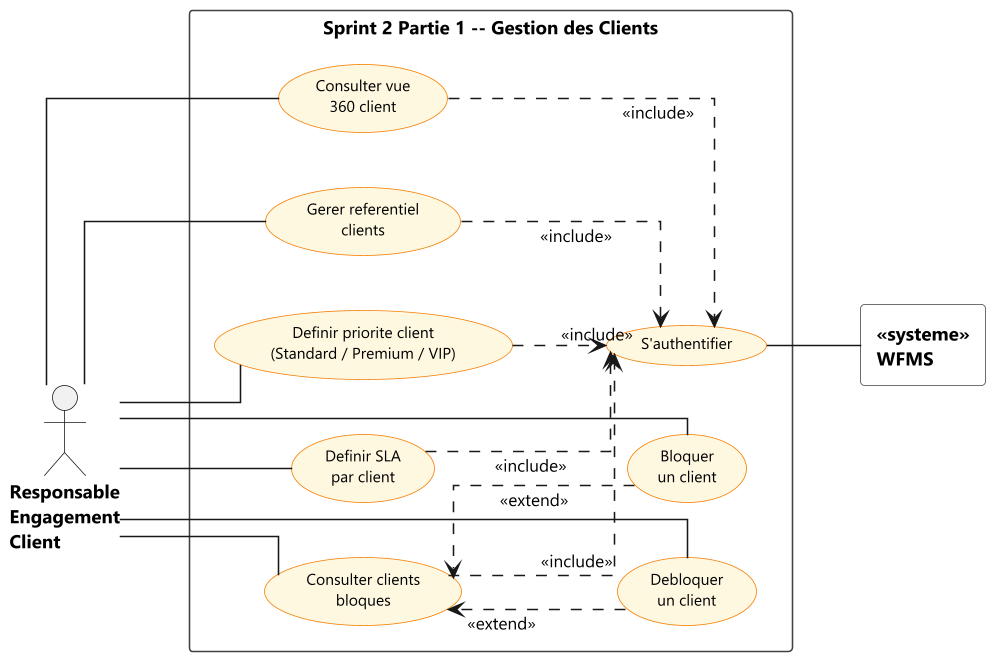
\includegraphics[width=0.9\textwidth, height=0.85\textheight, keepaspectratio]{img/diagrammes/sprint_2_usecase_p1}%
}{%
  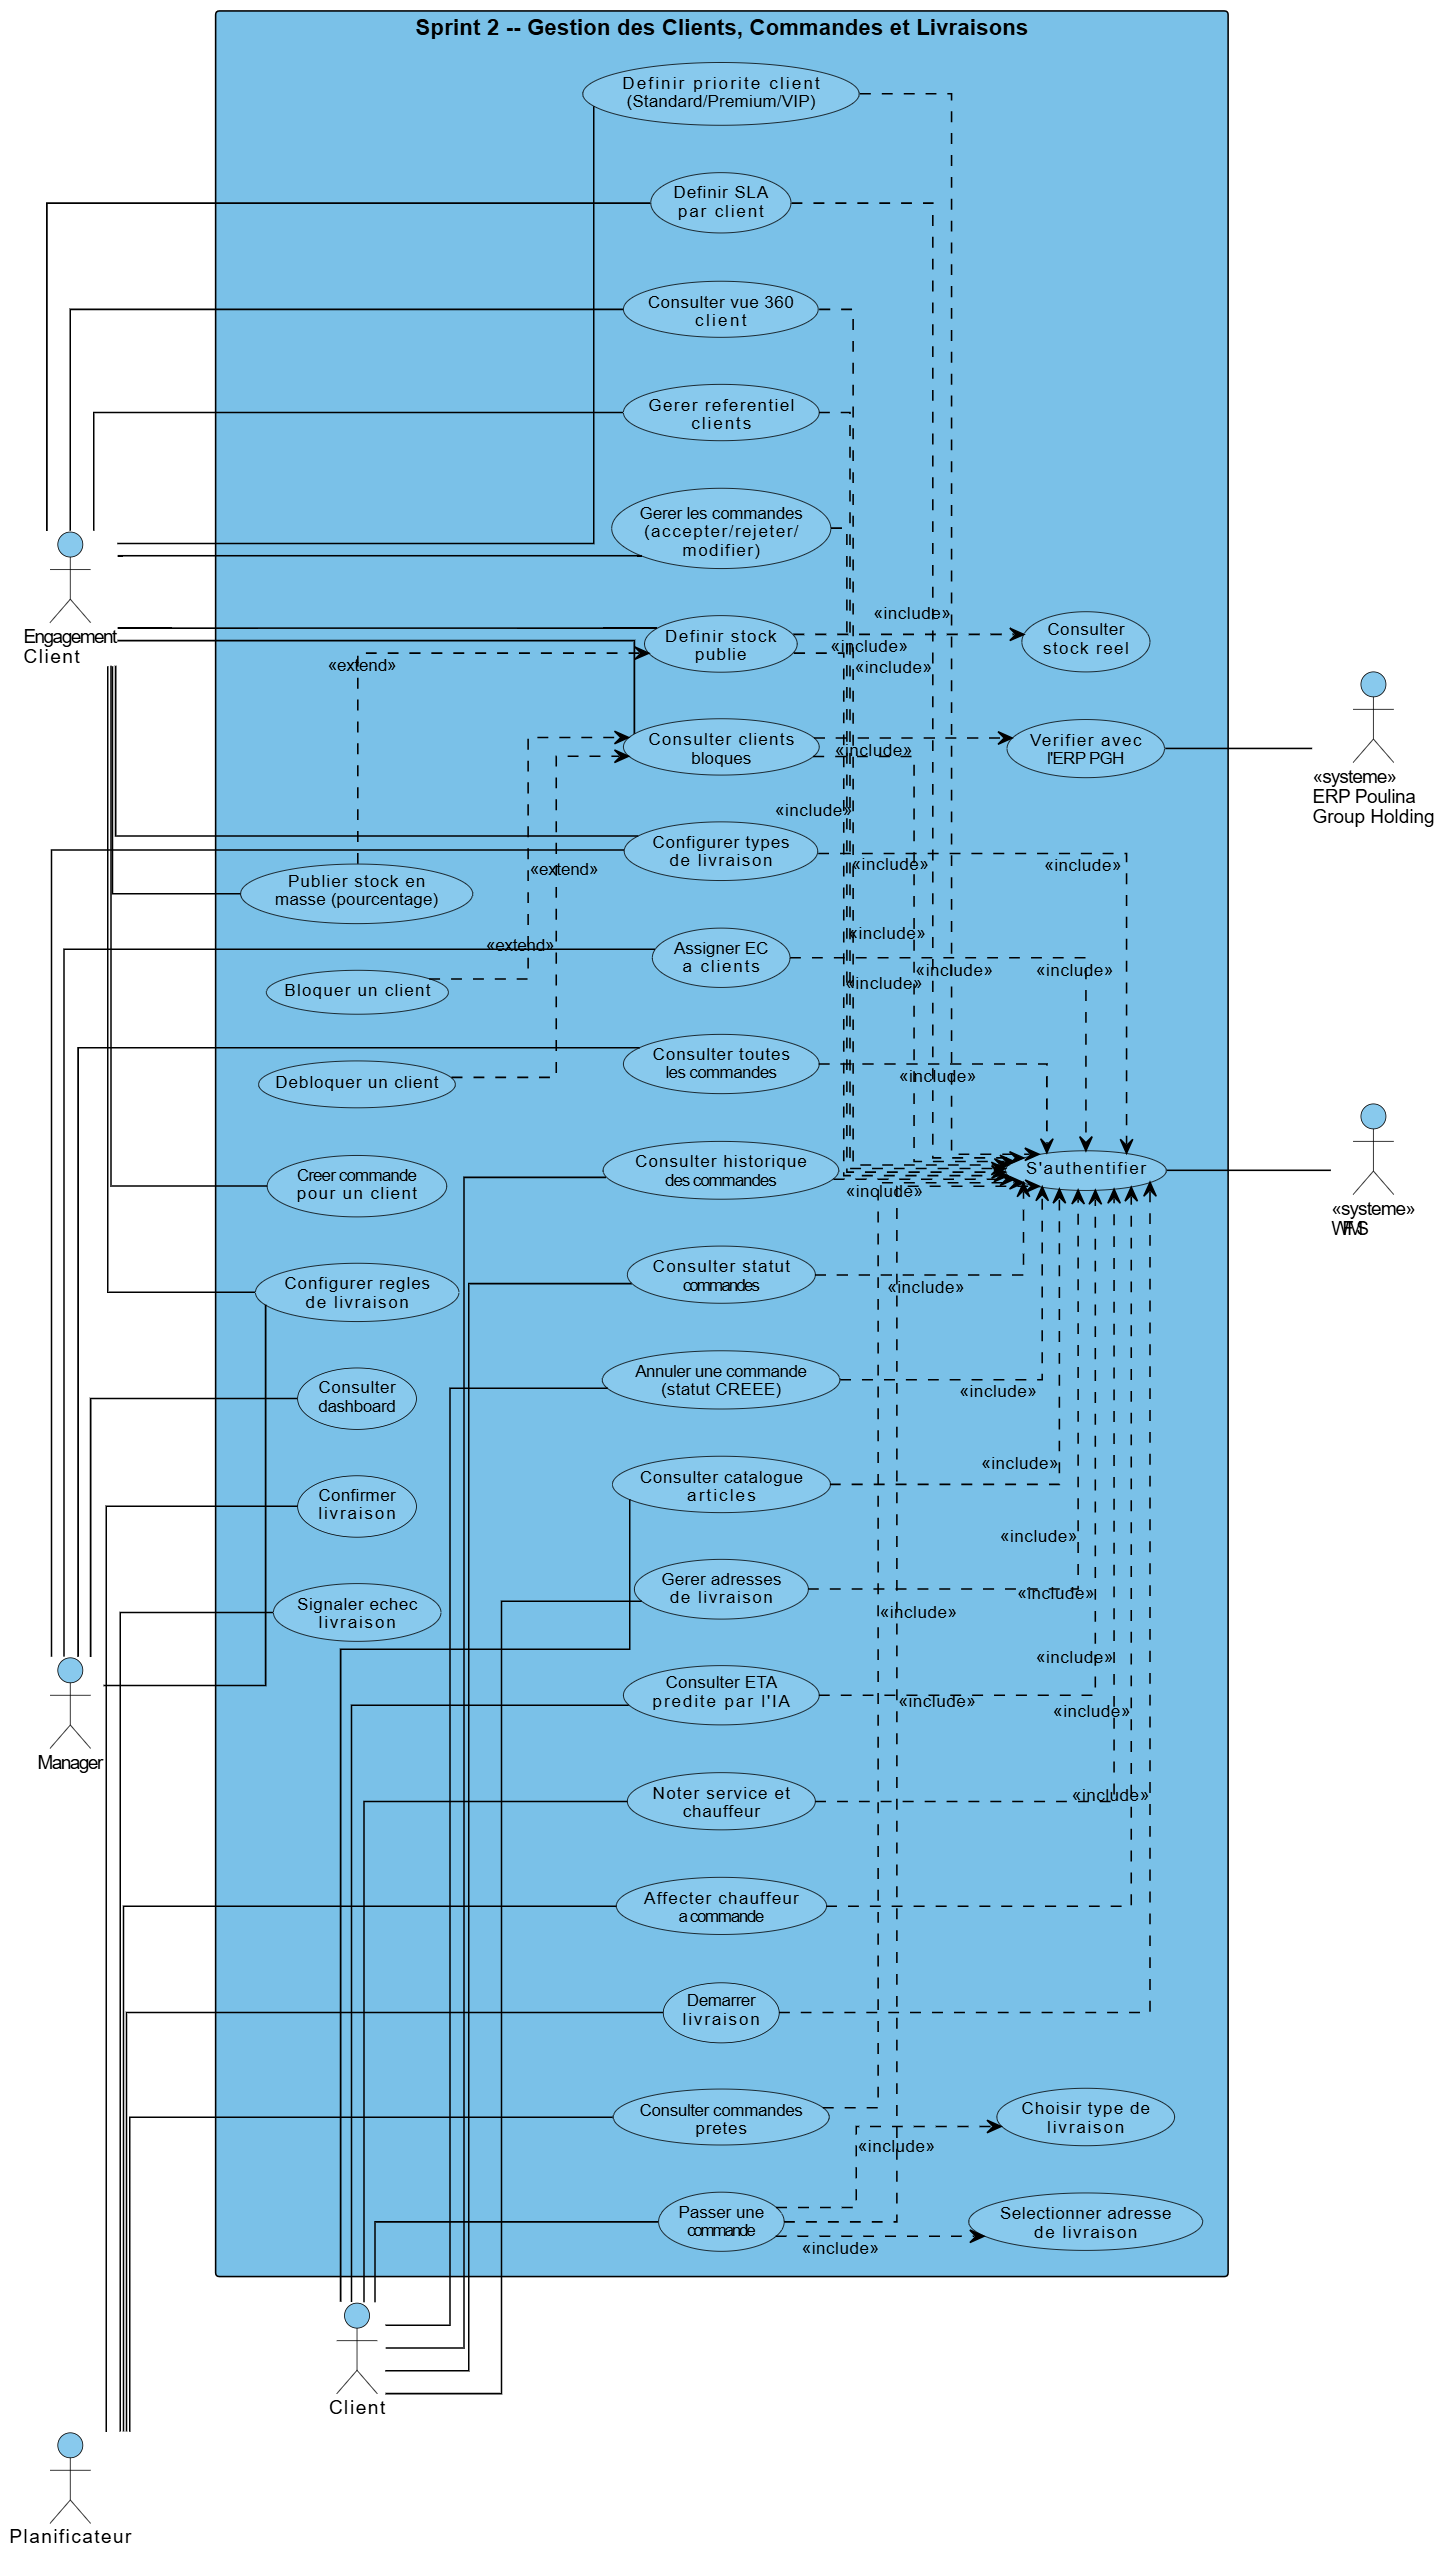
\includegraphics[width=0.9\textwidth, height=0.85\textheight, keepaspectratio]{img/diagrammes/sprint_2_usecase}%
}
\caption{Diagramme de cas d'utilisation du Sprint~2 --- Partie~1}
\label{fig:cas-utilisation-sp2-p1}
\end{figure}

\begin{figure}[H]
\centering
\IfFileExists{img/diagrammes/sprint_2_usecase_p2.png}{%
  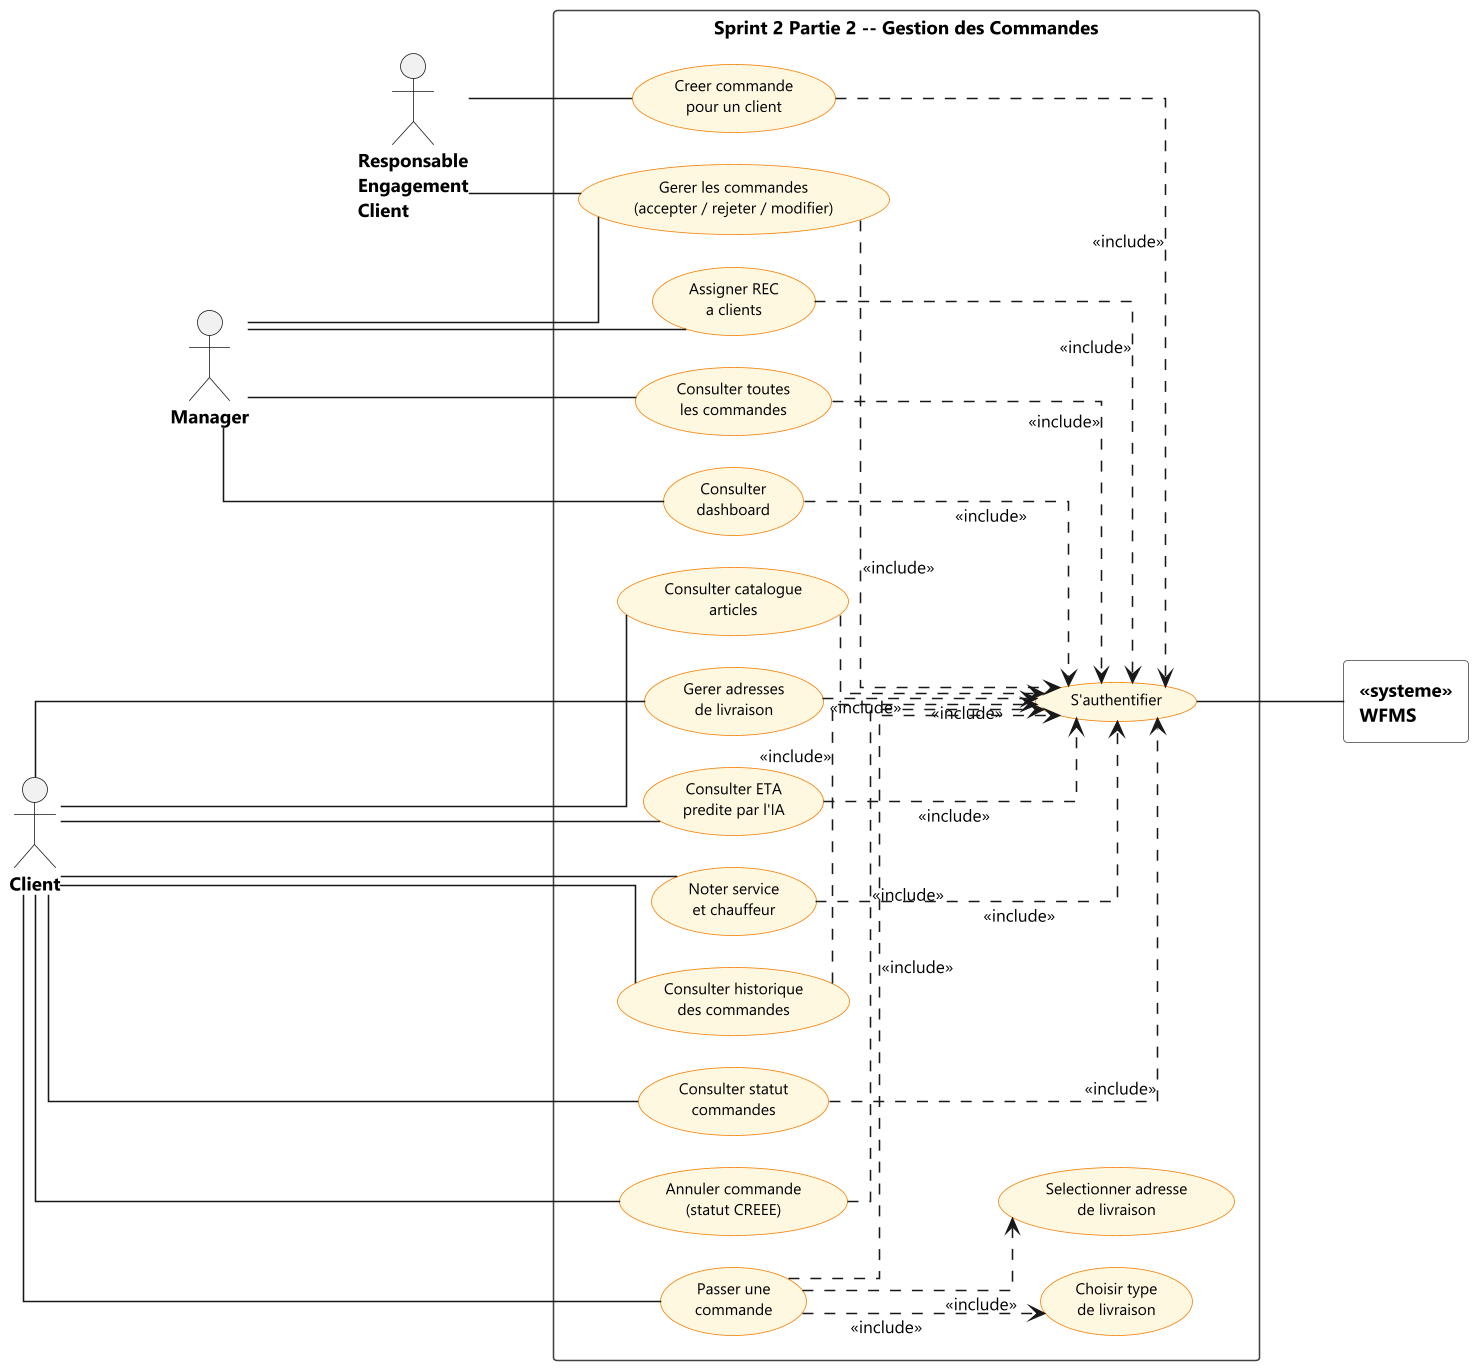
\includegraphics[width=0.9\textwidth, height=0.85\textheight, keepaspectratio]{img/diagrammes/sprint_2_usecase_p2}%
}{%
  \fbox{\parbox{0.9\linewidth}{\centering\vspace{1.5cm}\textit{[img/diagrammes/sprint\_2\_usecase\_p2.png]}\vspace{1.5cm}}}%
}
\caption{Diagramme de cas d'utilisation du Sprint~2 --- Partie~2}
\label{fig:cas-utilisation-sp2-p2}
\end{figure}

\begin{figure}[H]
\centering
\IfFileExists{img/diagrammes/sprint_2_usecase_p3.png}{%
  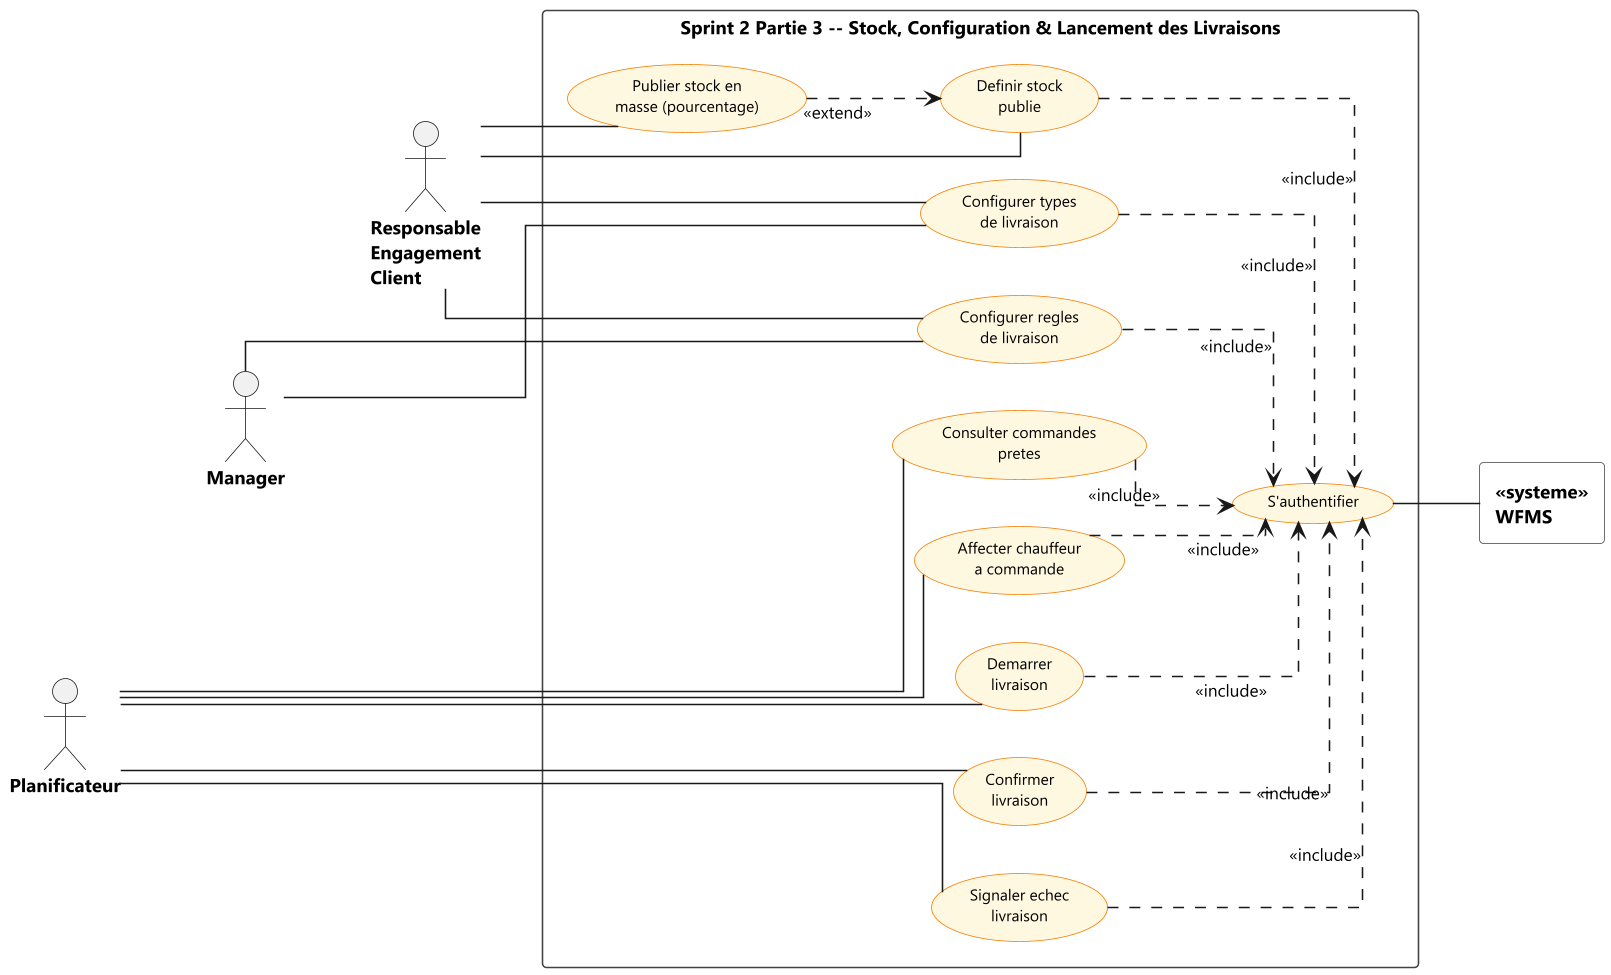
\includegraphics[width=0.9\textwidth, height=0.85\textheight, keepaspectratio]{img/diagrammes/sprint_2_usecase_p3}%
}{%
  \fbox{\parbox{0.9\linewidth}{\centering\vspace{1.5cm}\textit{[img/diagrammes/sprint\_2\_usecase\_p3.png]}\vspace{1.5cm}}}%
}
\caption{Diagramme de cas d'utilisation du Sprint~2 --- Partie~3}
\label{fig:cas-utilisation-sp2-p3}
\end{figure}

\subsection{Description textuelle}

\captionsetup[longtable]{justification=centering}
\setlength{\arrayrulewidth}{1pt}
\begin{longtable}{|p{4cm}|p{11cm}|}
\hline
\rowcolor{headerbg}
\textbf{Élément} & \textbf{Description} \\
\hline
\textbf{Titre} & Gérer les commandes \\
\hline
\textbf{Acteurs} & REC (parties 1, 2, 3), Manager (parties 2, 3), Client (partie 2), Planificateur (partie 3), Système WFMS \\
\hline
\textbf{Objectif} &
\begin{itemize}[nosep, leftmargin=1.4em]
    \item \textbf{P1 :} Maintenir le référentiel clients (vue~360, priorité Standard/Premium/VIP, SLA, blocage/déblocage).
    \item \textbf{P2 :} Gérer le cycle de vie des commandes (création, acceptation/rejet, suivi ETA par IA) pour le REC, le Manager et le Client.
    \item \textbf{P3 :} Configurer le stock et les règles de livraison, affecter les chauffeurs et lancer les missions.
\end{itemize} \\
\hline
\textbf{Précondition} & Tous les acteurs sont authentifiés via WFMS. Le catalogue produits, le stock et les règles de livraison sont disponibles. \\
\hline
\textbf{Postcondition} & Le référentiel clients est à jour~; la commande est transmise à l'ERP (statut ACCEPTÉE)~; les livraisons sont affectées et leur statut (confirmée ou échec) est enregistré. \\
\hline
\textbf{Scénario nominal} &
\begin{enumerate}[start=1, label=\arabic*., nosep, leftmargin=1.4em]
    \item Le REC met à jour la priorité et le SLA du client depuis la vue~360.
    \item Le Client passe une commande~; le REC la crée, vérifie le stock et l'accepte (statut ACCEPTÉE) — la commande est envoyée à l'ERP.
    \item Le Manager pilote via le dashboard~; le Client suit l'état et consulte l'ETA prédit par IA.
    \item Le REC publie le stock en masse et configure les règles/types de livraison.
    \item Le Planificateur consulte les commandes prêtes, affecte un chauffeur, démarre et confirme la livraison.
\end{enumerate} \\
\hline
\textbf{Scénario alternatif} &
\begin{enumerate}[start=1, label=\arabic*., nosep, leftmargin=1.4em]
    \item Client bloqué : commande refusée~; le REC peut débloquer après régularisation.
    \item Stock insuffisant : création bloquée~; le REC publie une mise à jour de stock en masse.
    \item Commande rejetée par le REC : le Client est notifié et peut l'annuler (statut CRÉÉE uniquement).
    \item Échec de livraison : le Planificateur le signale~; la mission est replanifiée.
\end{enumerate} \\
\hline
\caption{Description textuelle --- Gérer les commandes (Sprint 2)}
\end{longtable}
\setlength{\arrayrulewidth}{0.4pt}

\subsection{Cycle de vie d'une commande}

La figure~\ref{fig:cycle-vie-commande-sp2} illustre le cycle de vie complet d'une commande Fleet AI depuis sa création jusqu'à la livraison, en montrant les interactions entre le Client, le REC, l'ERP Poulina et le système de livraison.

\begin{figure}[H]
\centering
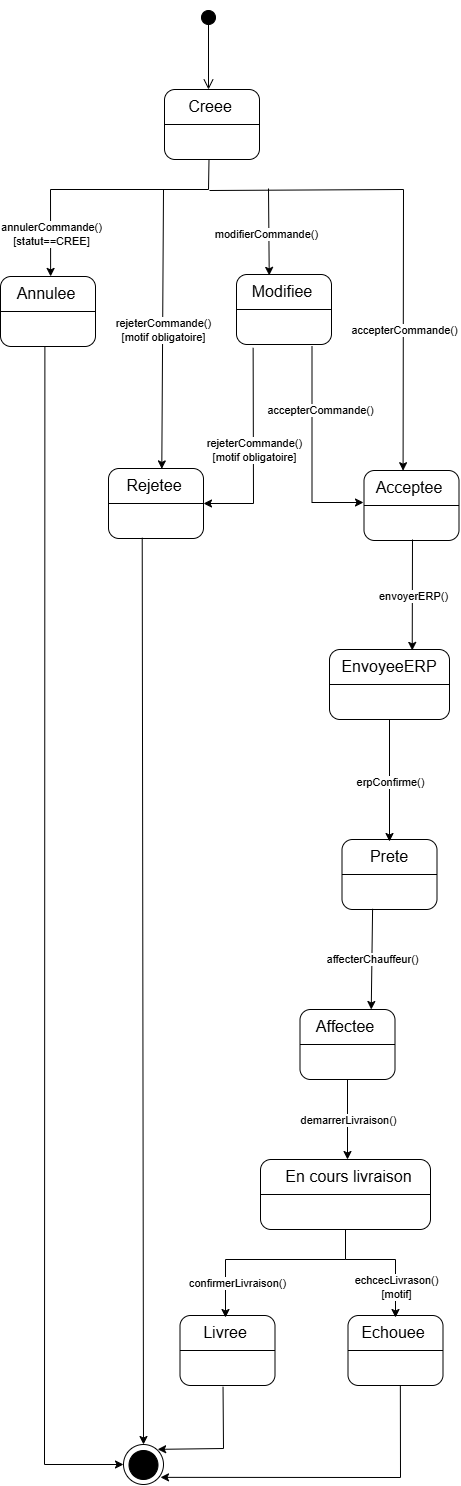
\includegraphics[width=\textwidth, height=0.7\textheight, keepaspectratio]{img/diagrammes/sprint2_cycleVieCommande}
\caption{Cycle de vie complet d'une commande Fleet AI}
\label{fig:cycle-vie-commande-sp2}
\end{figure}

\subsection{Diagramme de classes}

\newpage
\thispagestyle{empty}
\begin{landscape}
\begin{figure}[H]
\centering
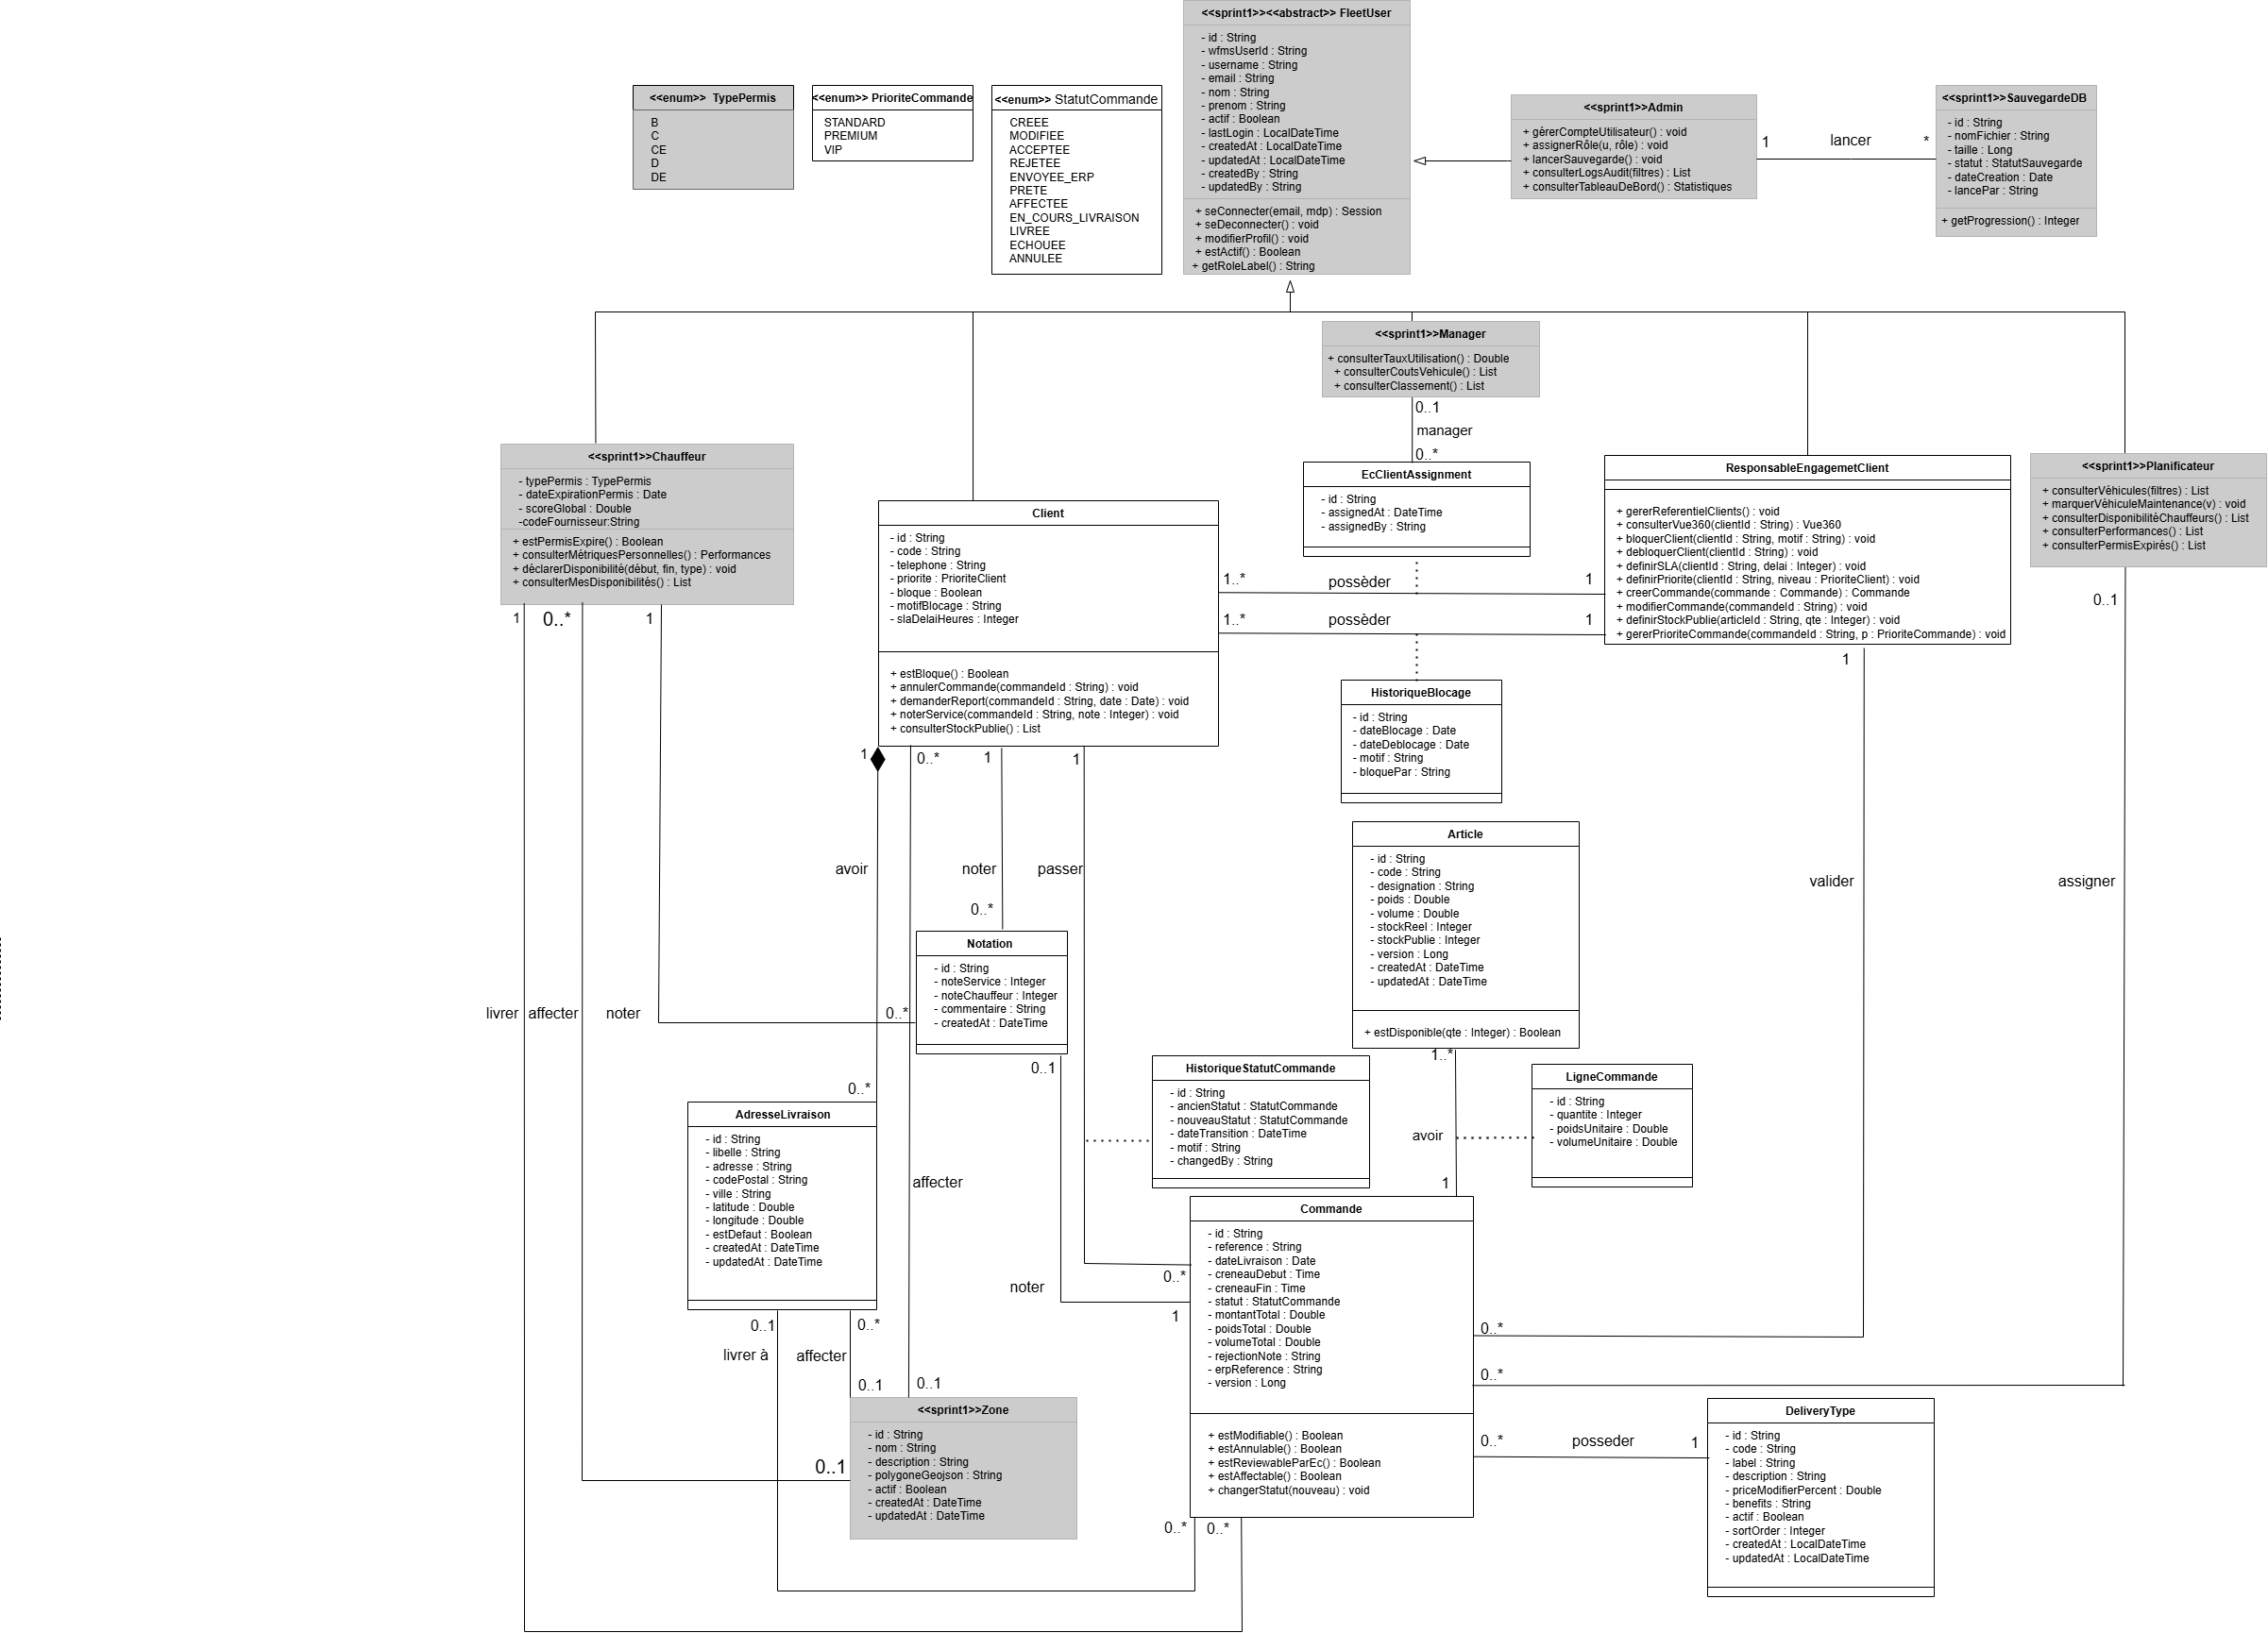
\includegraphics[width=\linewidth, height=0.95\textheight, keepaspectratio]{img/diagrammes/sprint_2_classes}
\caption{Diagramme de classes du Sprint 2}
\label{fig:diag-classes-sp2}
\end{figure}
\end{landscape}

% =============================================================
\section{Réalisation}
% =============================================================

\subsection{Gestion des clients et adresses de livraison}

Le REC gère son portefeuille via une liste paginable avec filtres. La Vue 360° d'un client regroupe ses commandes, ses adresses et son historique de blocage. Le blocage est immédiat avec motif obligatoire. Le REC gère également les adresses de livraison de ses clients, avec détection automatique de la zone de livraison à partir des coordonnées GPS (algorithme Ray-Casting). Une seule adresse peut être marquée comme adresse par défaut.

\begin{figure}[H]
\centering
\IfFileExists{img/capture/web/sp2_clients_composite.png}{%
  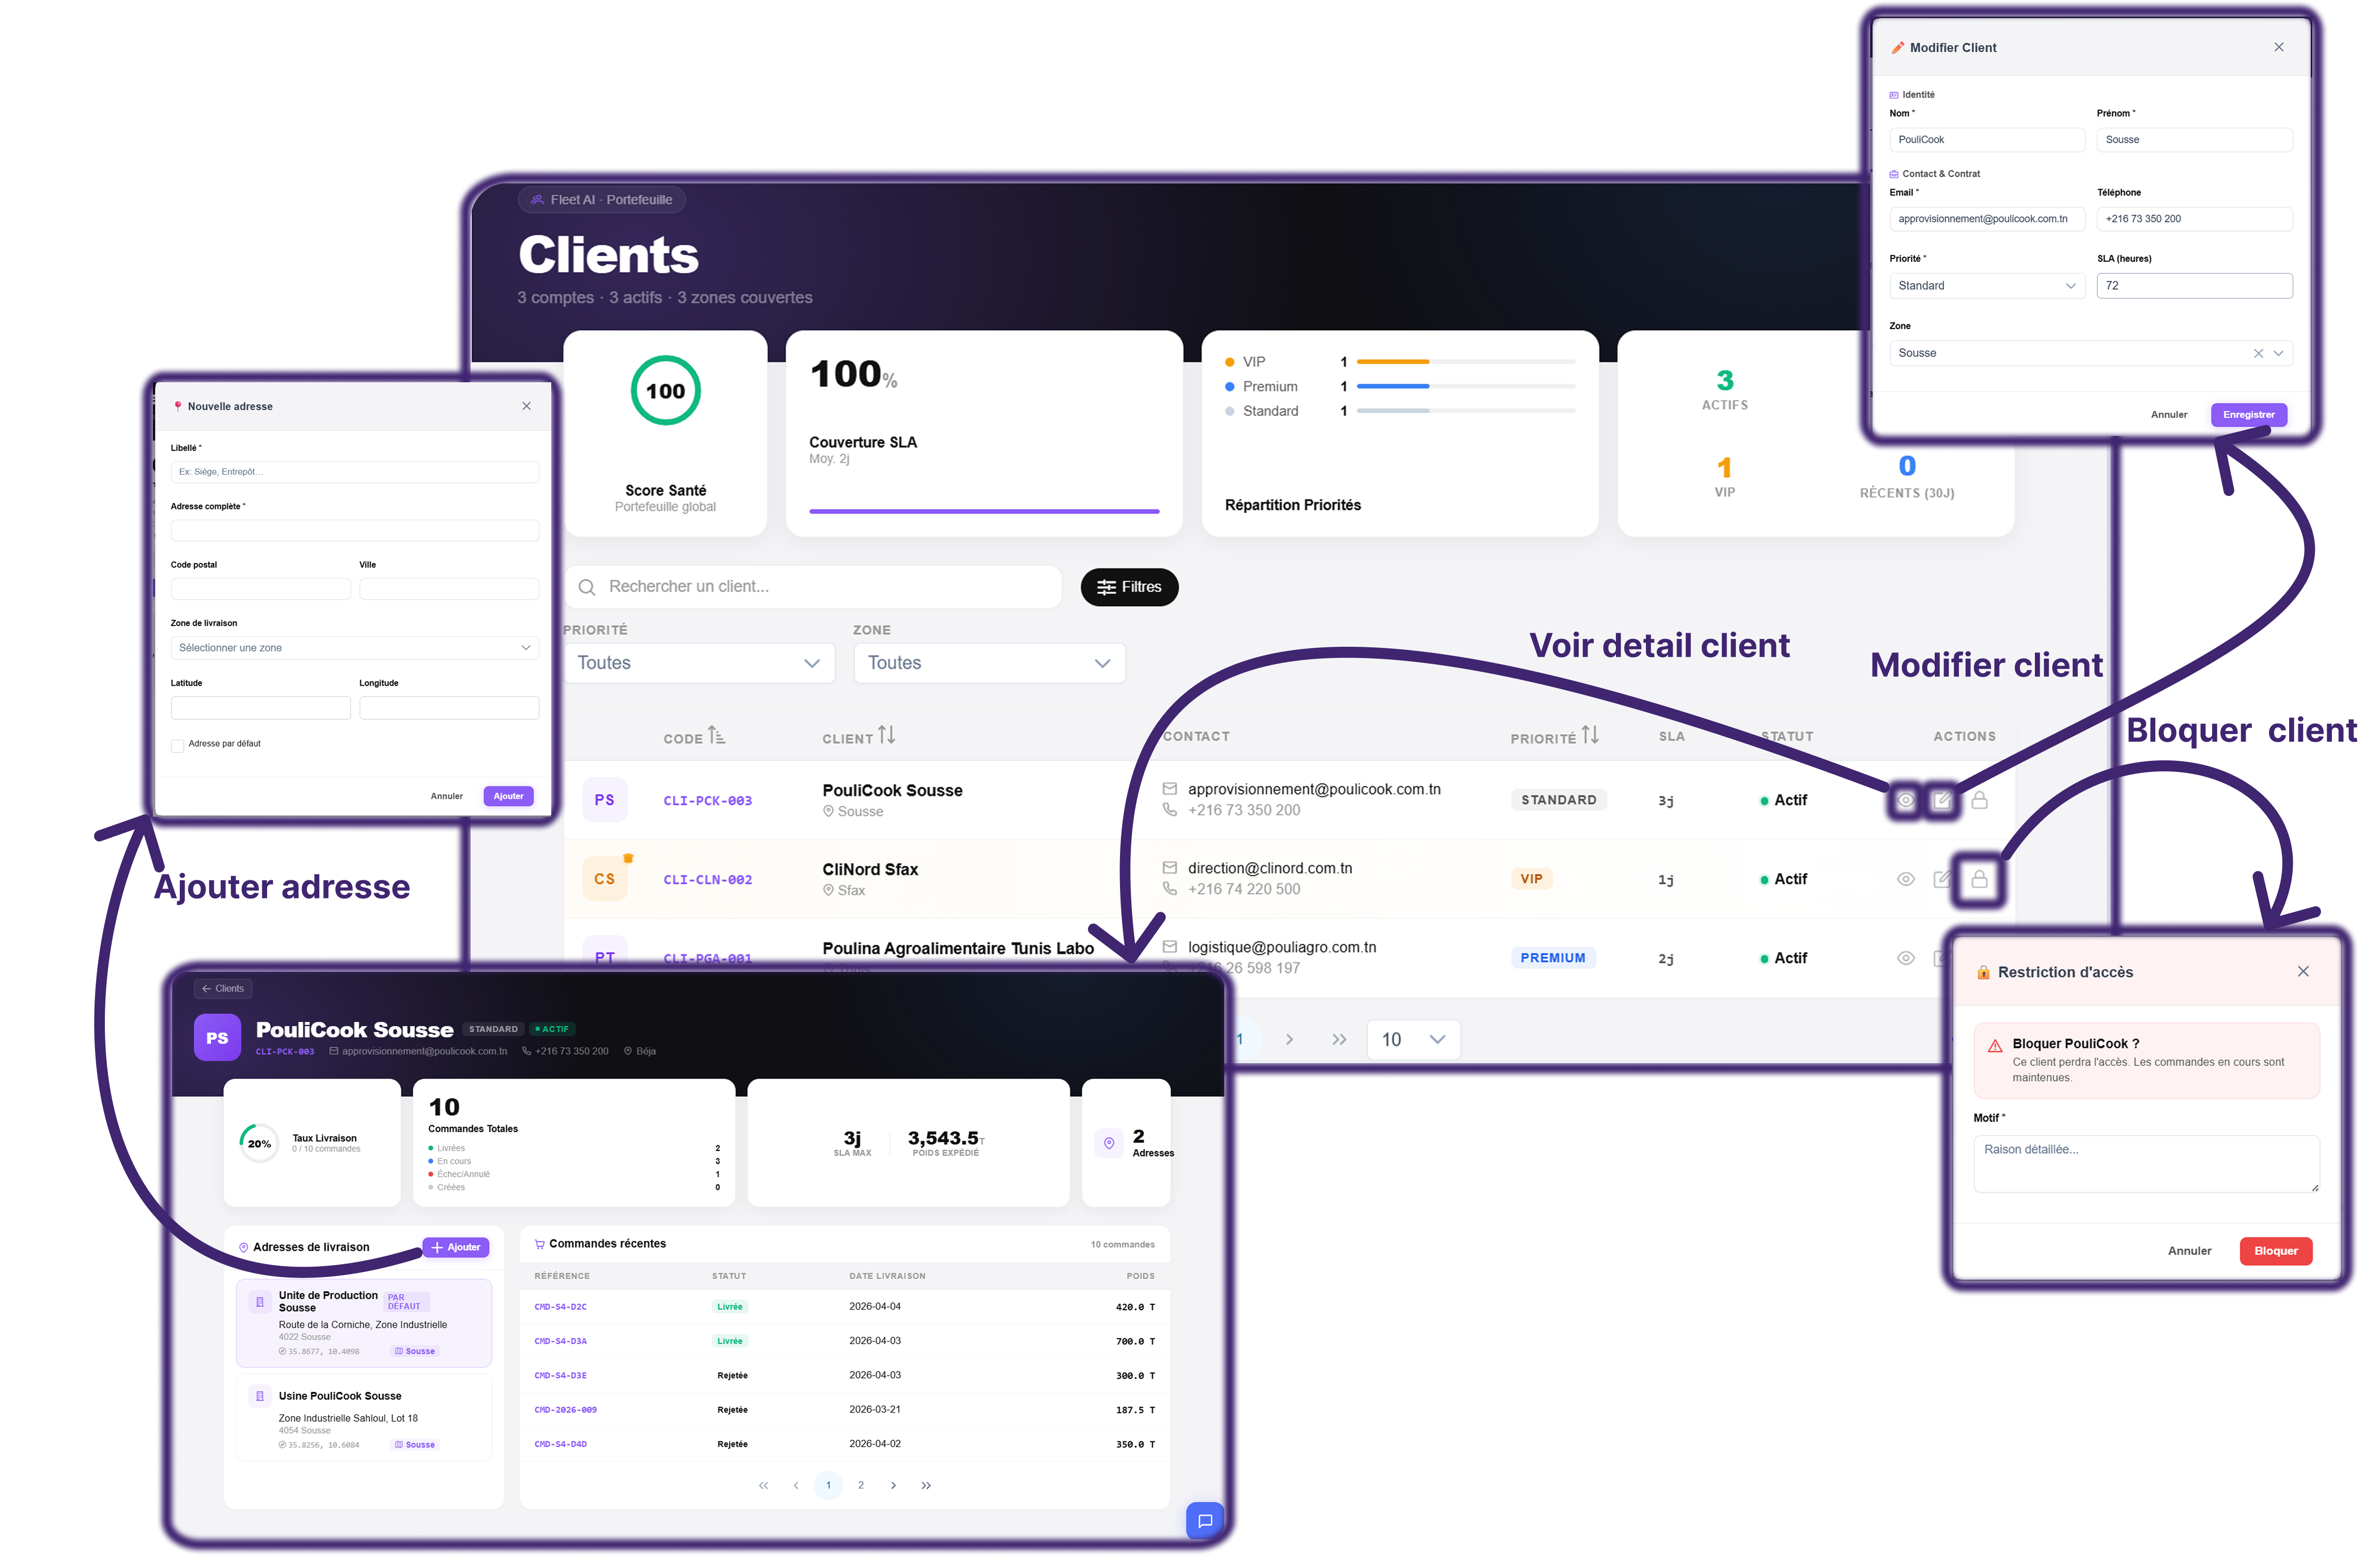
\includegraphics[width=\linewidth, keepaspectratio]{img/capture/web/sp2_clients_composite}%
}{%
  \fbox{\parbox{0.9\linewidth}{\centering\vspace{1.5cm}\textit{[img/sp2\_clients\_composite]}\vspace{1.5cm}}}%
}
\caption{Gestion clients : Vue 360°, blocage et adresses GPS}
\label{fig:sp2-clients-addresses}
\end{figure}

\subsection{Catalogue et gestion du stock}

Deux niveaux de stock coexistent : le stock réel (visible REC uniquement) et le stock publié (visible Client). Le REC fixe manuellement le stock publié dans la limite du stock réel.

\begin{figure}[H]
\centering
\IfFileExists{img/capture/web/sp2_stock_composite.png}{%
  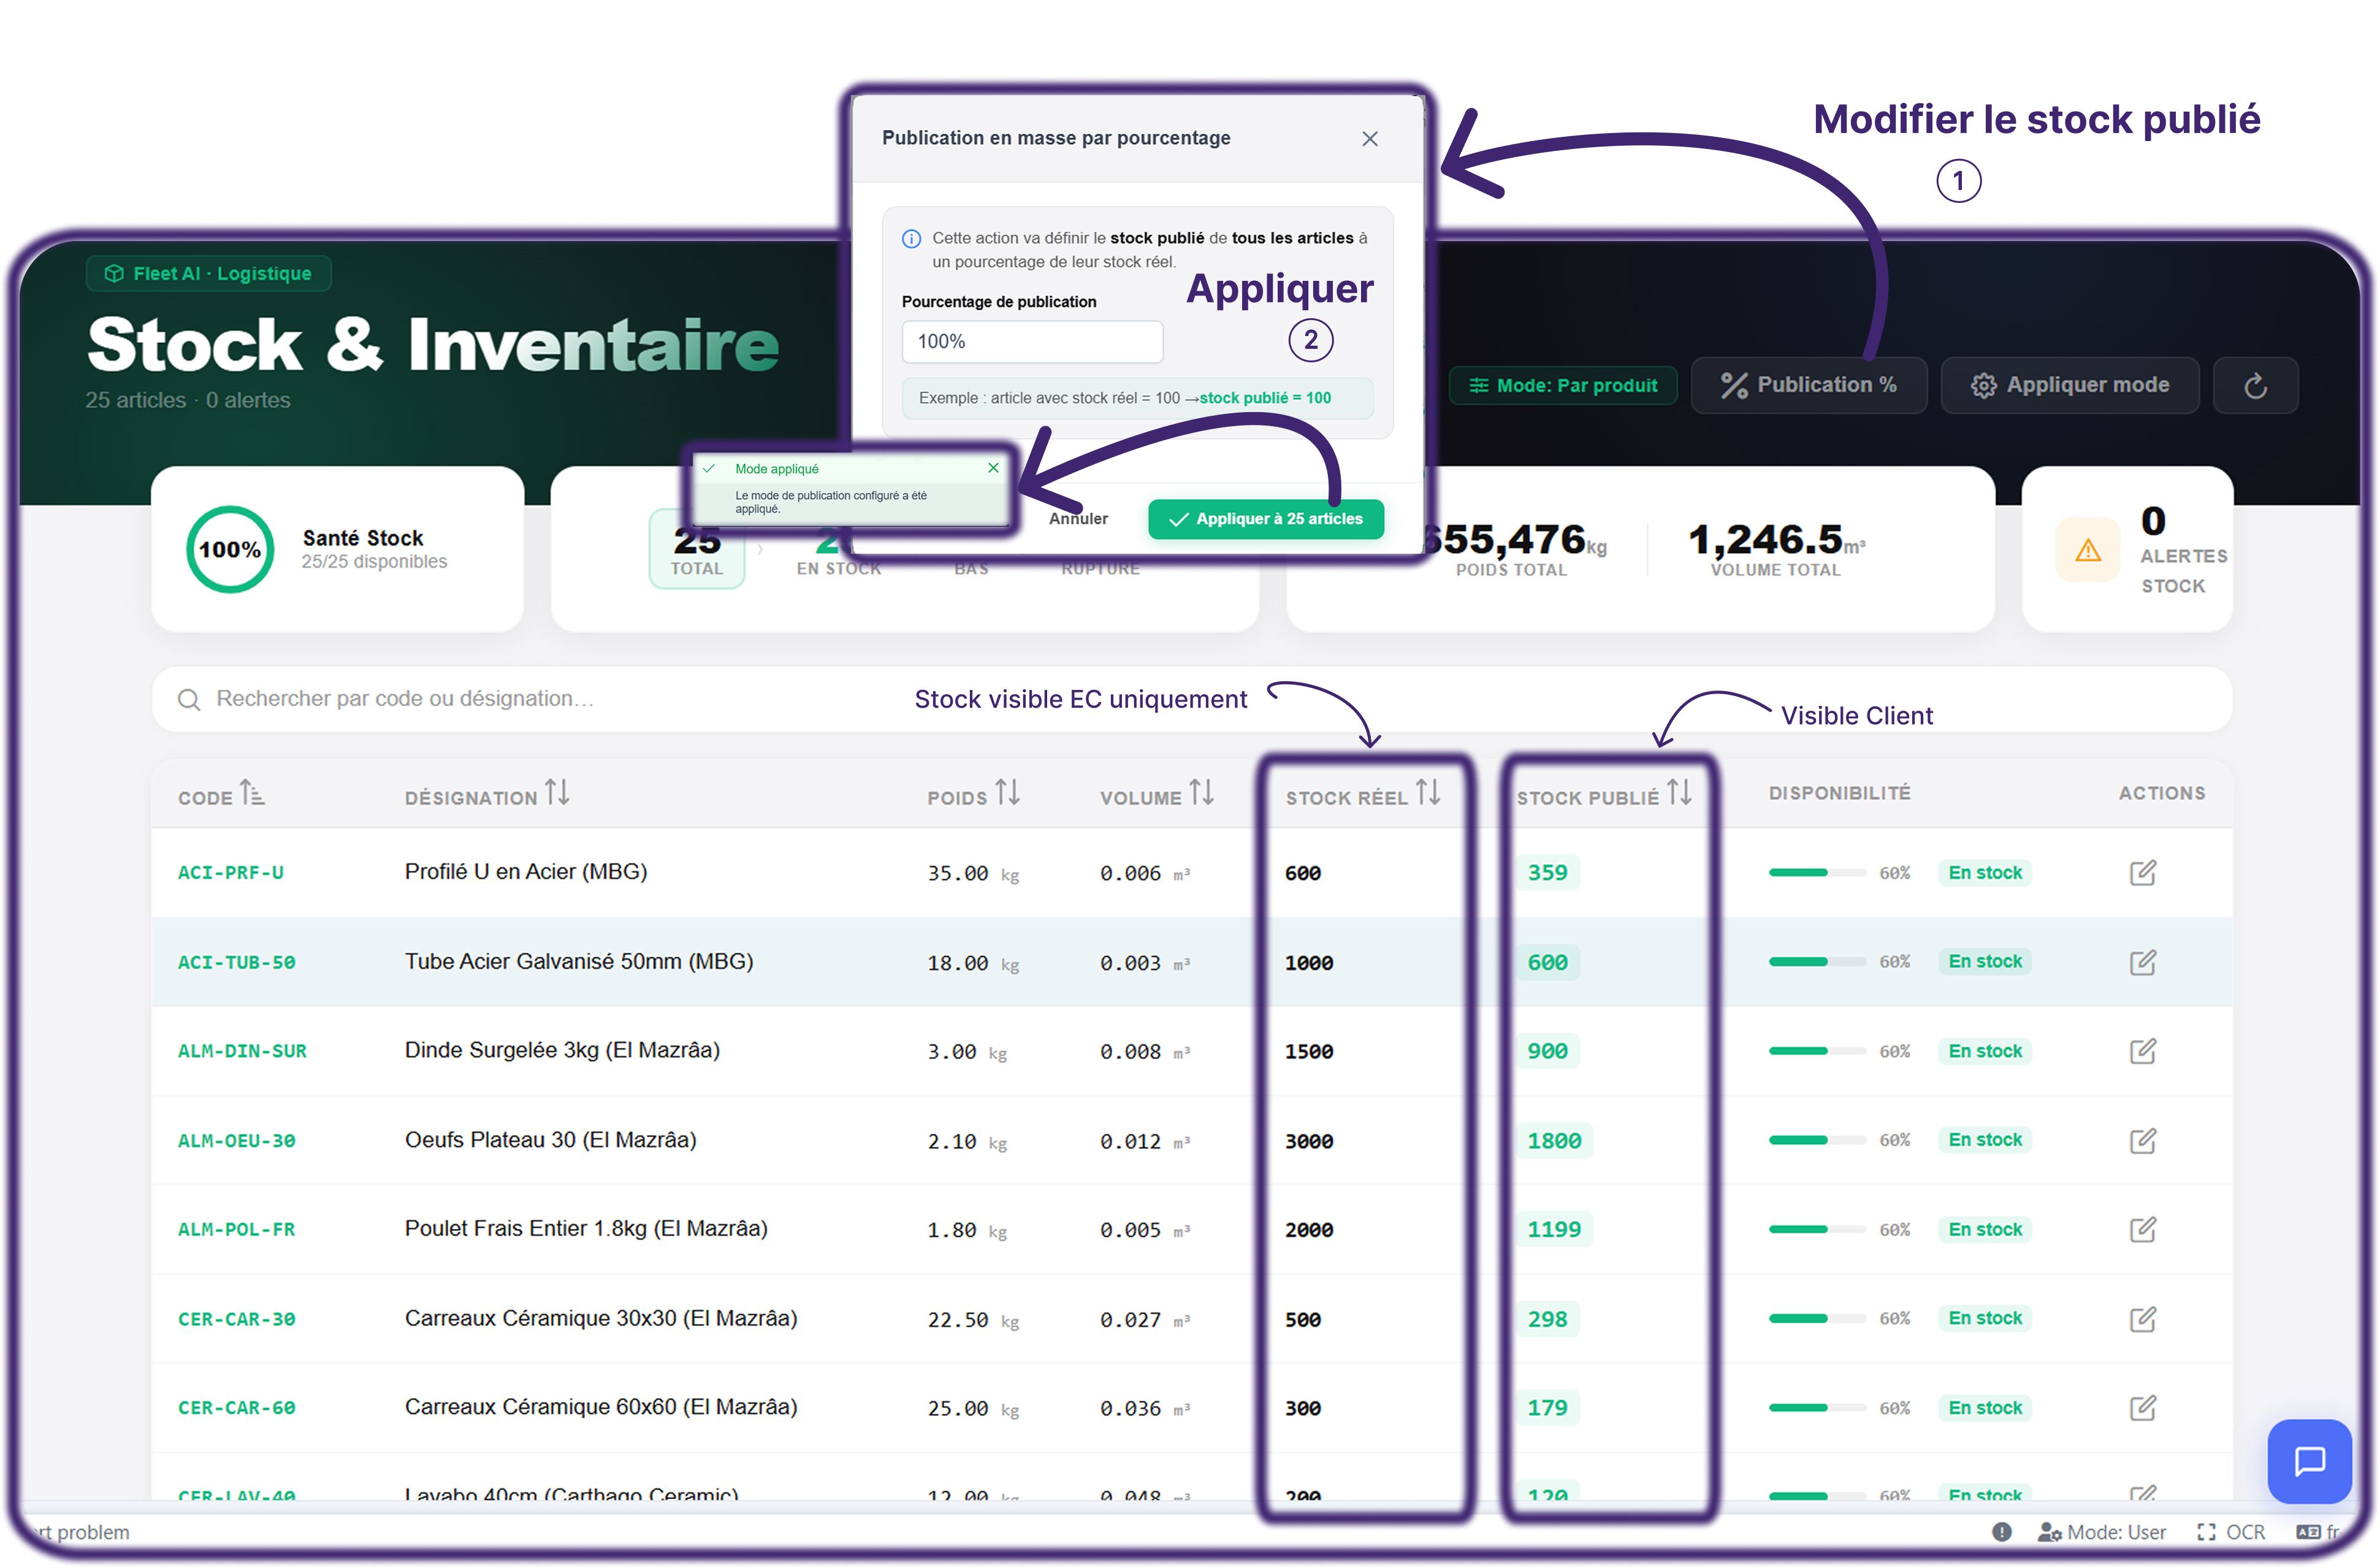
\includegraphics[width=\linewidth, keepaspectratio]{img/capture/web/sp2_stock_composite}%
}{%
  \fbox{\parbox{0.9\linewidth}{\centering\vspace{1.5cm}\textit{[img/sp2\_stock\_composite]}\vspace{1.5cm}}}%
}
\caption{Catalogue : niveaux stock réel et publié}
\label{fig:sp2-stock}
\end{figure}

\subsection{Gestion des commandes}

La création d'une commande vérifie le statut de blocage du client et la disponibilité du stock. La commande suit un cycle de vie strict à dix statuts, chaque transition tracée avec acteur et horodatage.

\begin{figure}[H]
\centering
\IfFileExists{img/capture/web/sp2_orders_composite.png}{%
  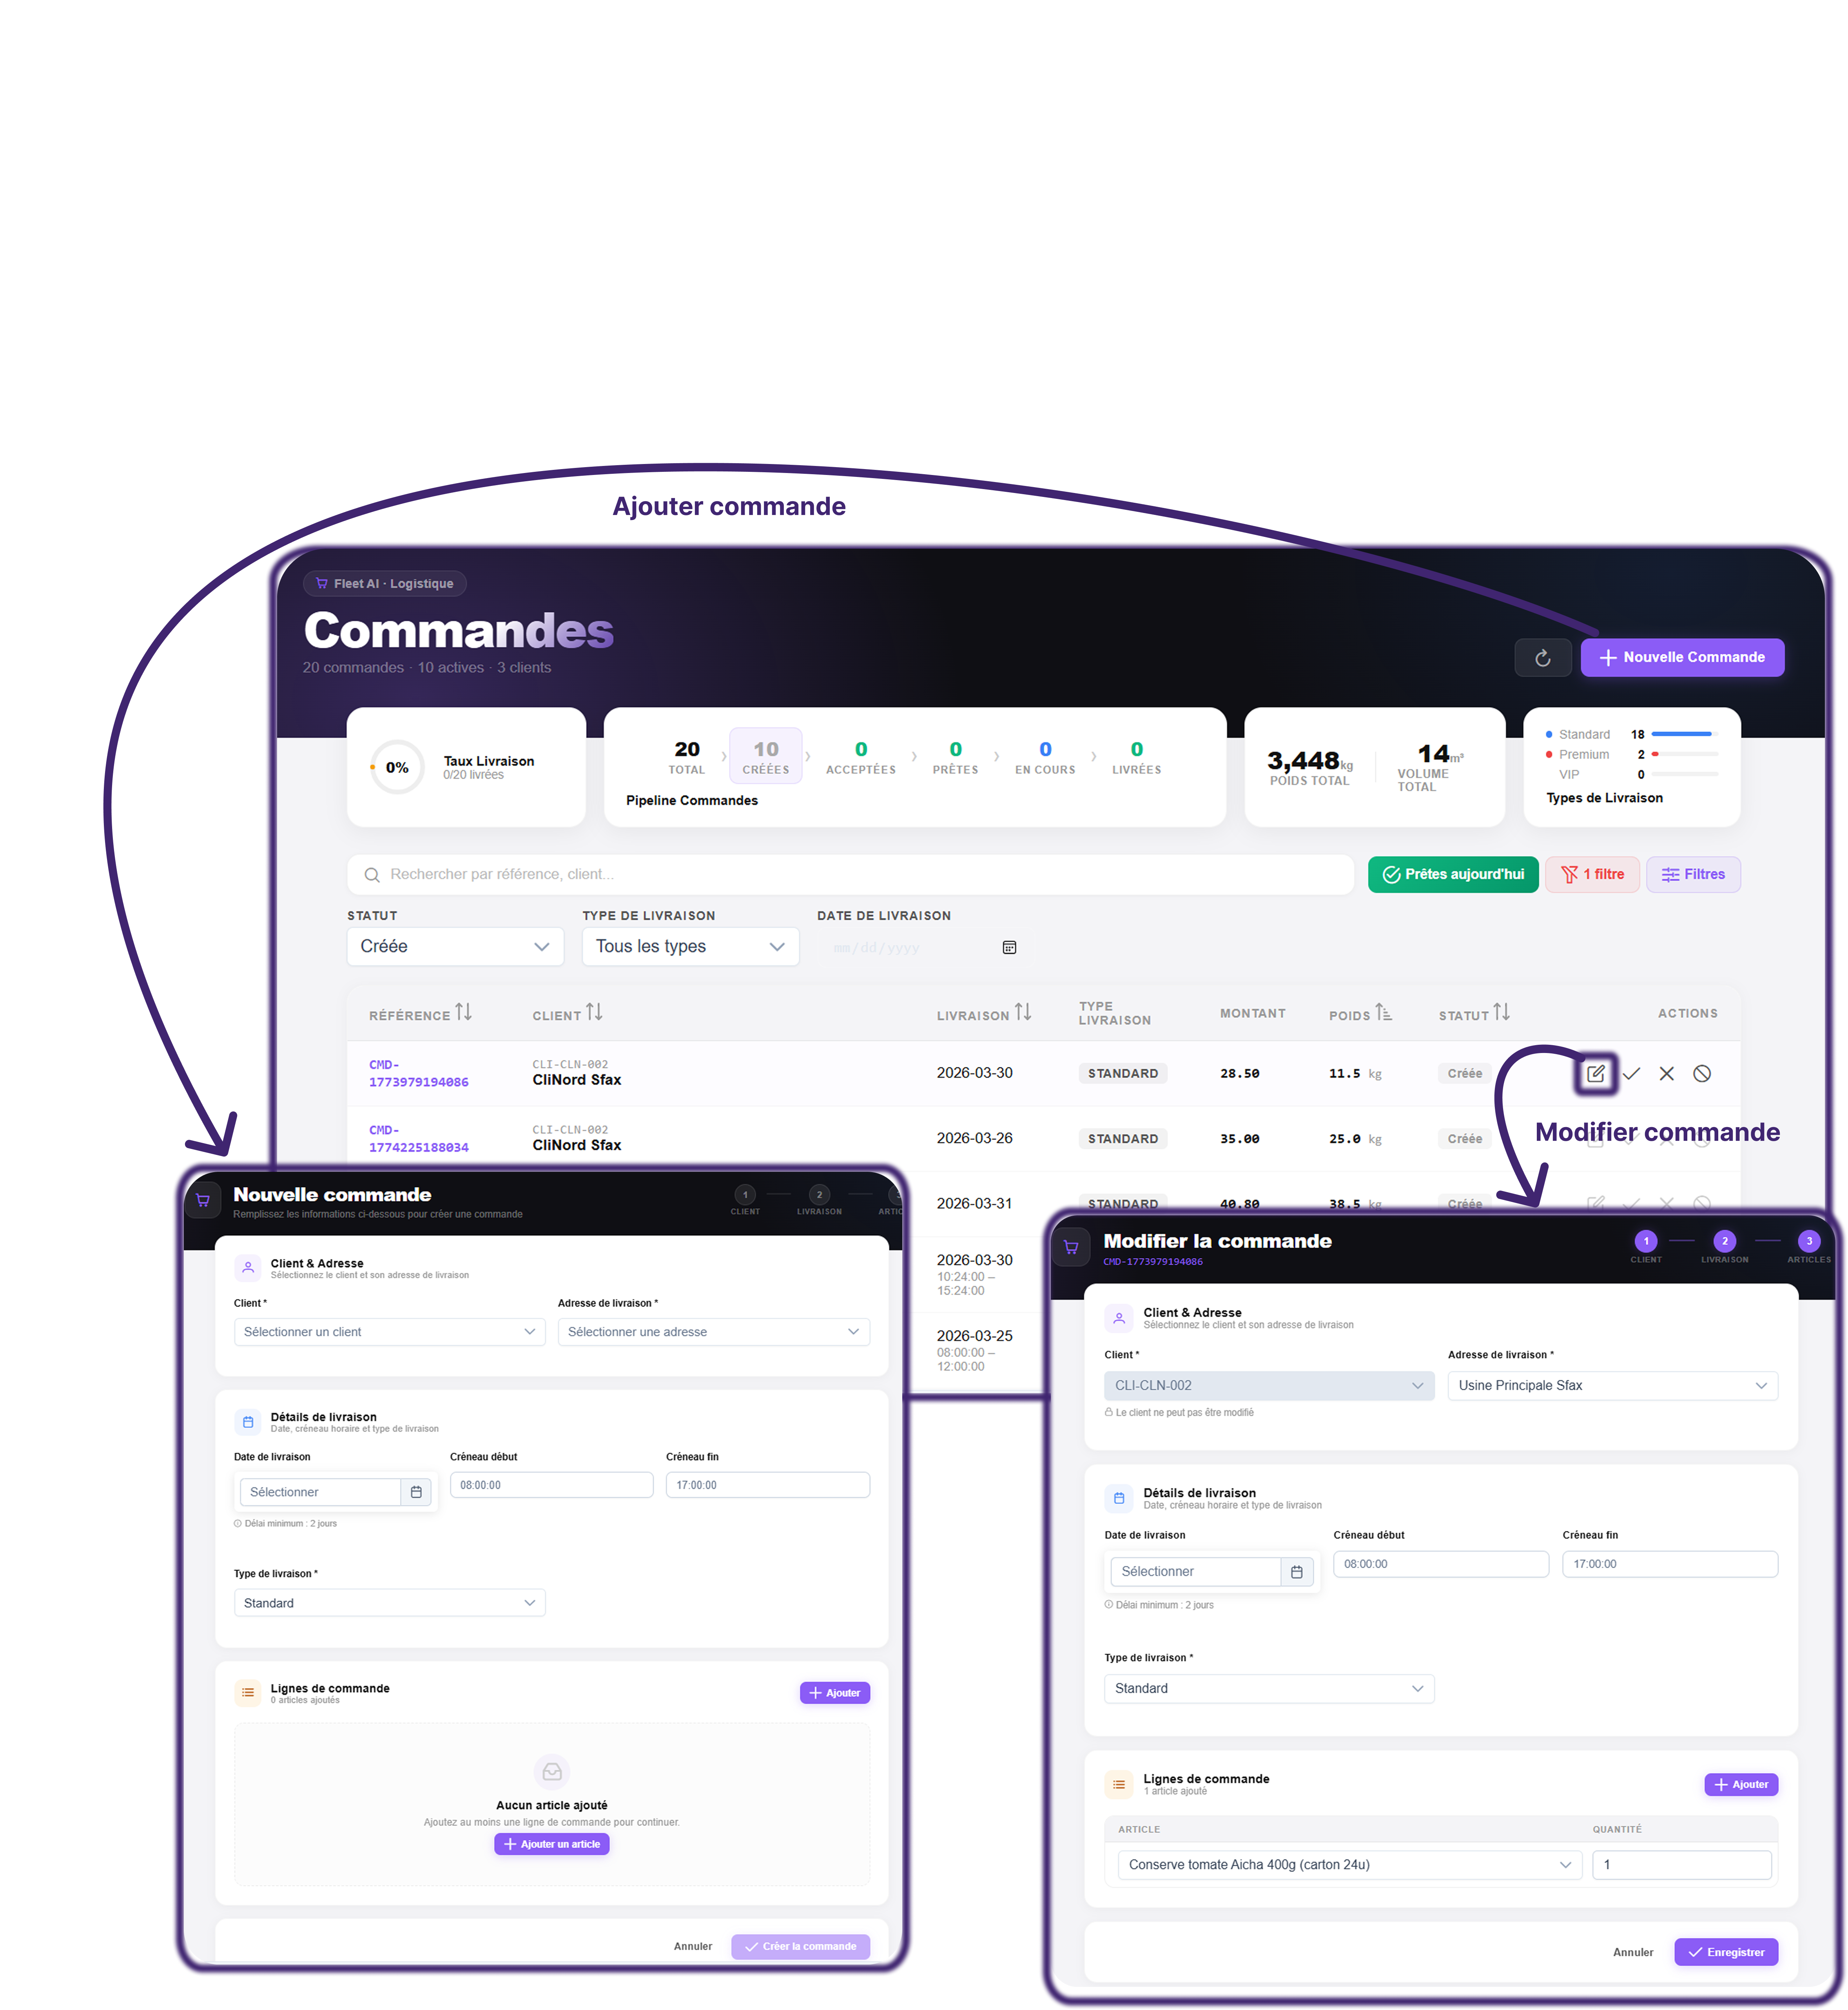
\includegraphics[width=\linewidth, keepaspectratio]{img/capture/web/sp2_orders_composite}%
}{%
  \fbox{\parbox{0.9\linewidth}{\centering\vspace{1.5cm}\textit{[img/sp2\_orders\_composite]}\vspace{1.5cm}}}%
}
\caption{Commandes : badge de statut et formulaire de création}
\label{fig:sp2-orders}
\end{figure}

\subsection{Affectation REC-Client}

Le Manager définit les périmètres de responsabilité en assignant des clients à des REC. Un client ne peut être assigné qu'à un seul REC à la fois. Les affectations et désaffectations en lot sont possibles depuis l'interface dédiée.

\begin{figure}[H]
\centering
\IfFileExists{img/capture/web/sp2_ec_assignments_composite.png}{%
  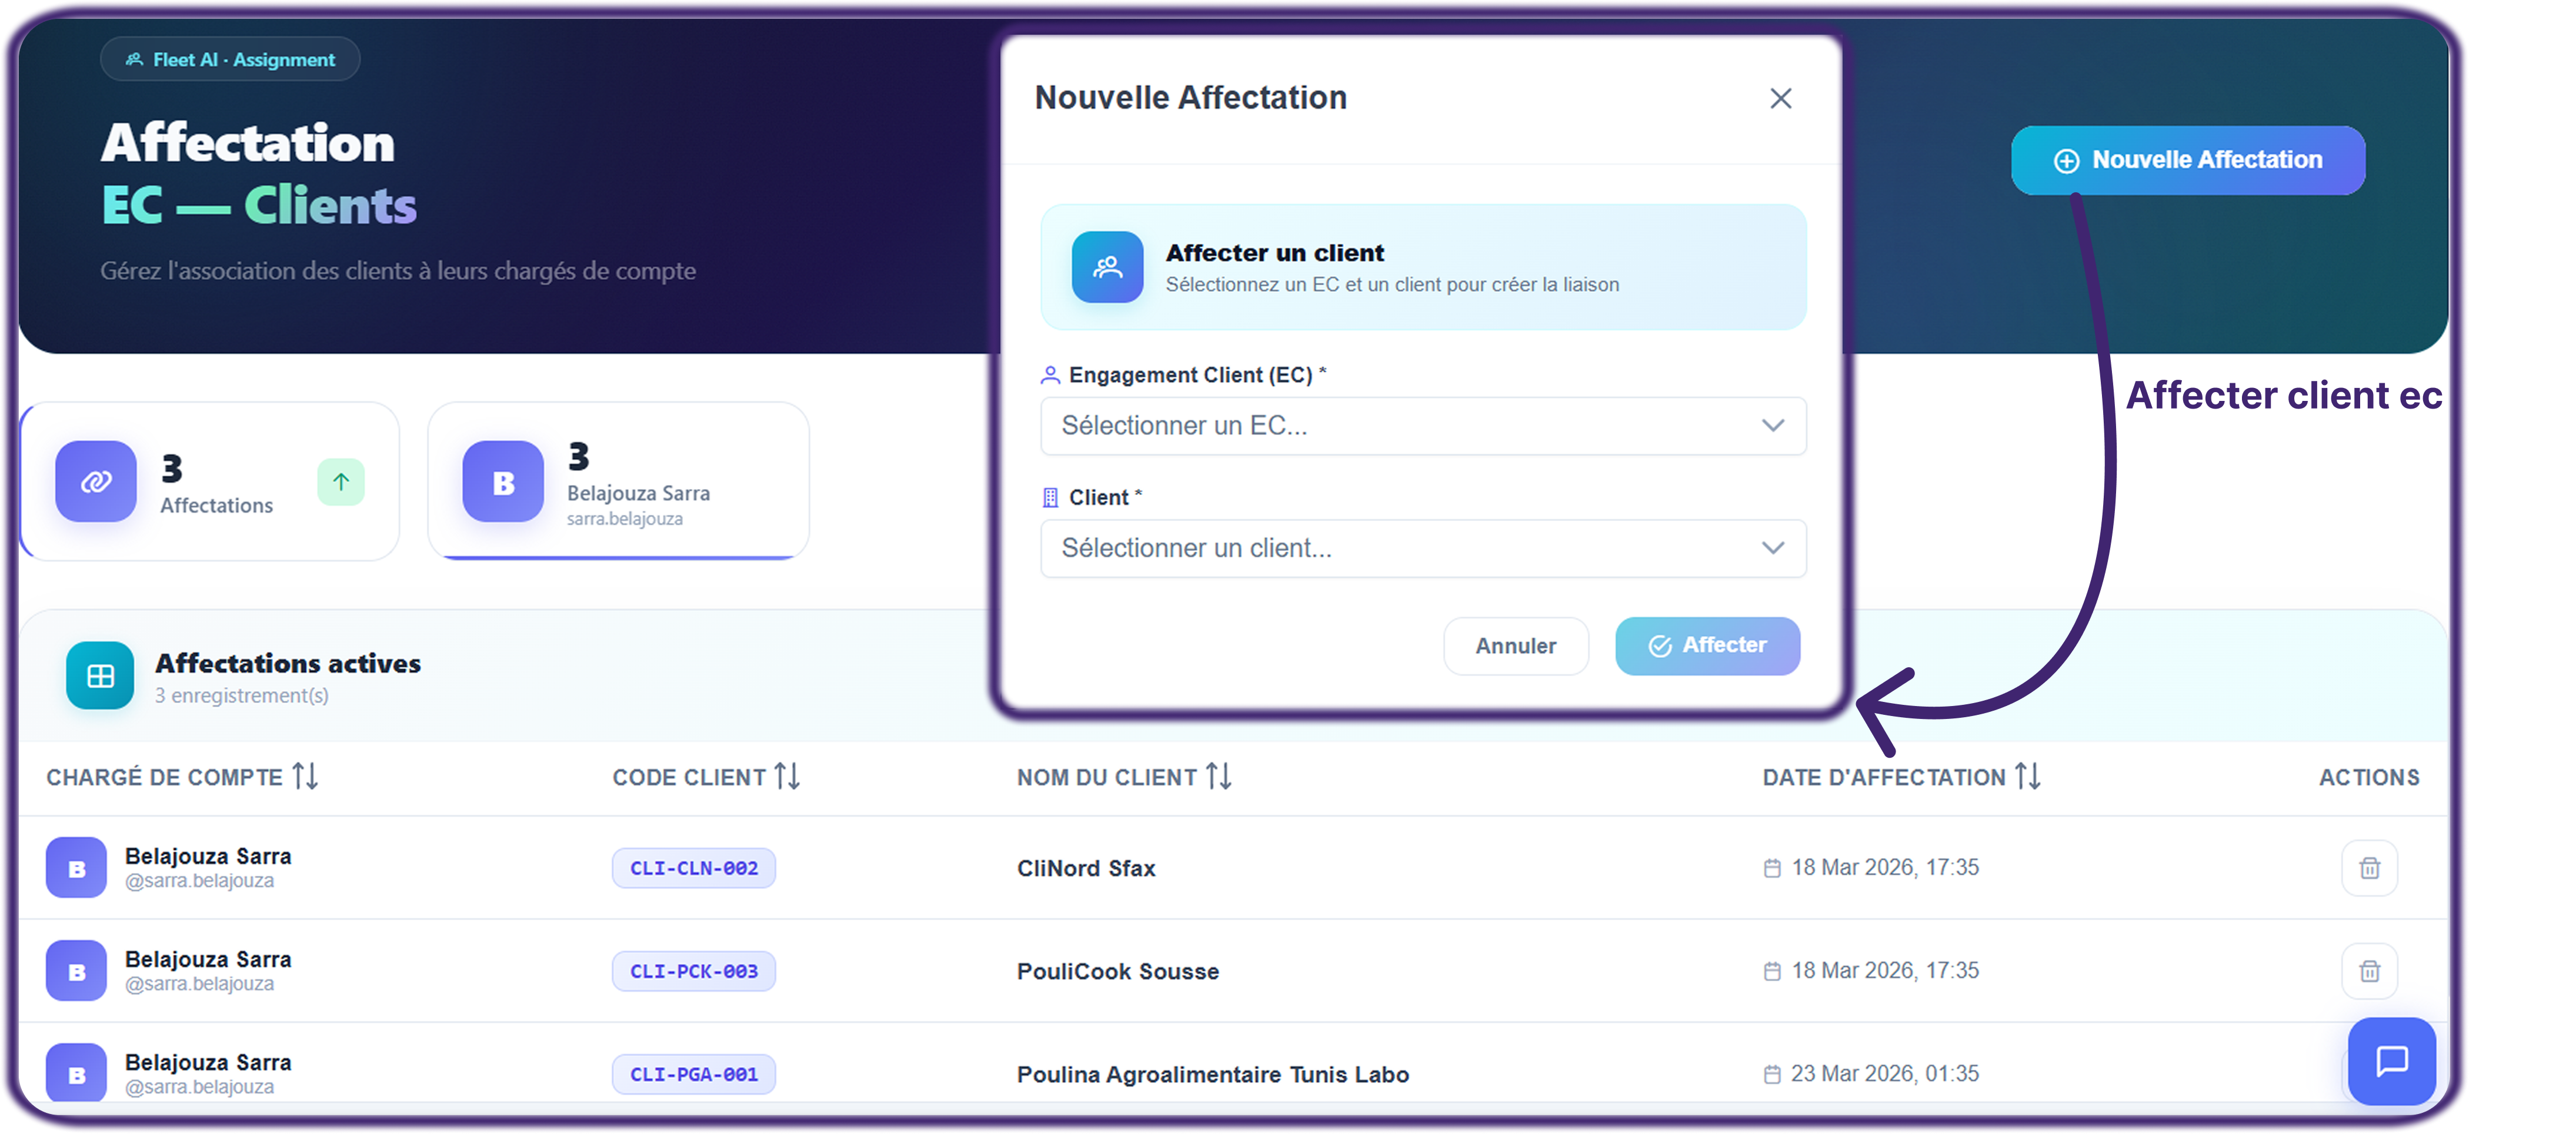
\includegraphics[width=\linewidth, keepaspectratio]{img/capture/web/sp2_ec_assignments_composite}%
}{%
  \fbox{\parbox{0.9\linewidth}{\centering\vspace{1.5cm}\textit{[img/sp2\_ec\_assignments\_composite]}\vspace{1.5cm}}}%
}
\caption{Affectation REC-Client en lot}
\label{fig:sp2-ec-assign}
\end{figure}

\subsection{Application mobile Client (Flutter)}

L'application mobile permet au Client de parcourir le catalogue d'articles, de passer des commandes via un workflow en quatre étapes (catalogue \textrightarrow{} panier \textrightarrow{} adresse \textrightarrow{} type~\&~date de livraison \textrightarrow{} confirmation), et de suivre ses commandes actives avec leur statut en temps réel.

\begin{figure}[H]
\centering
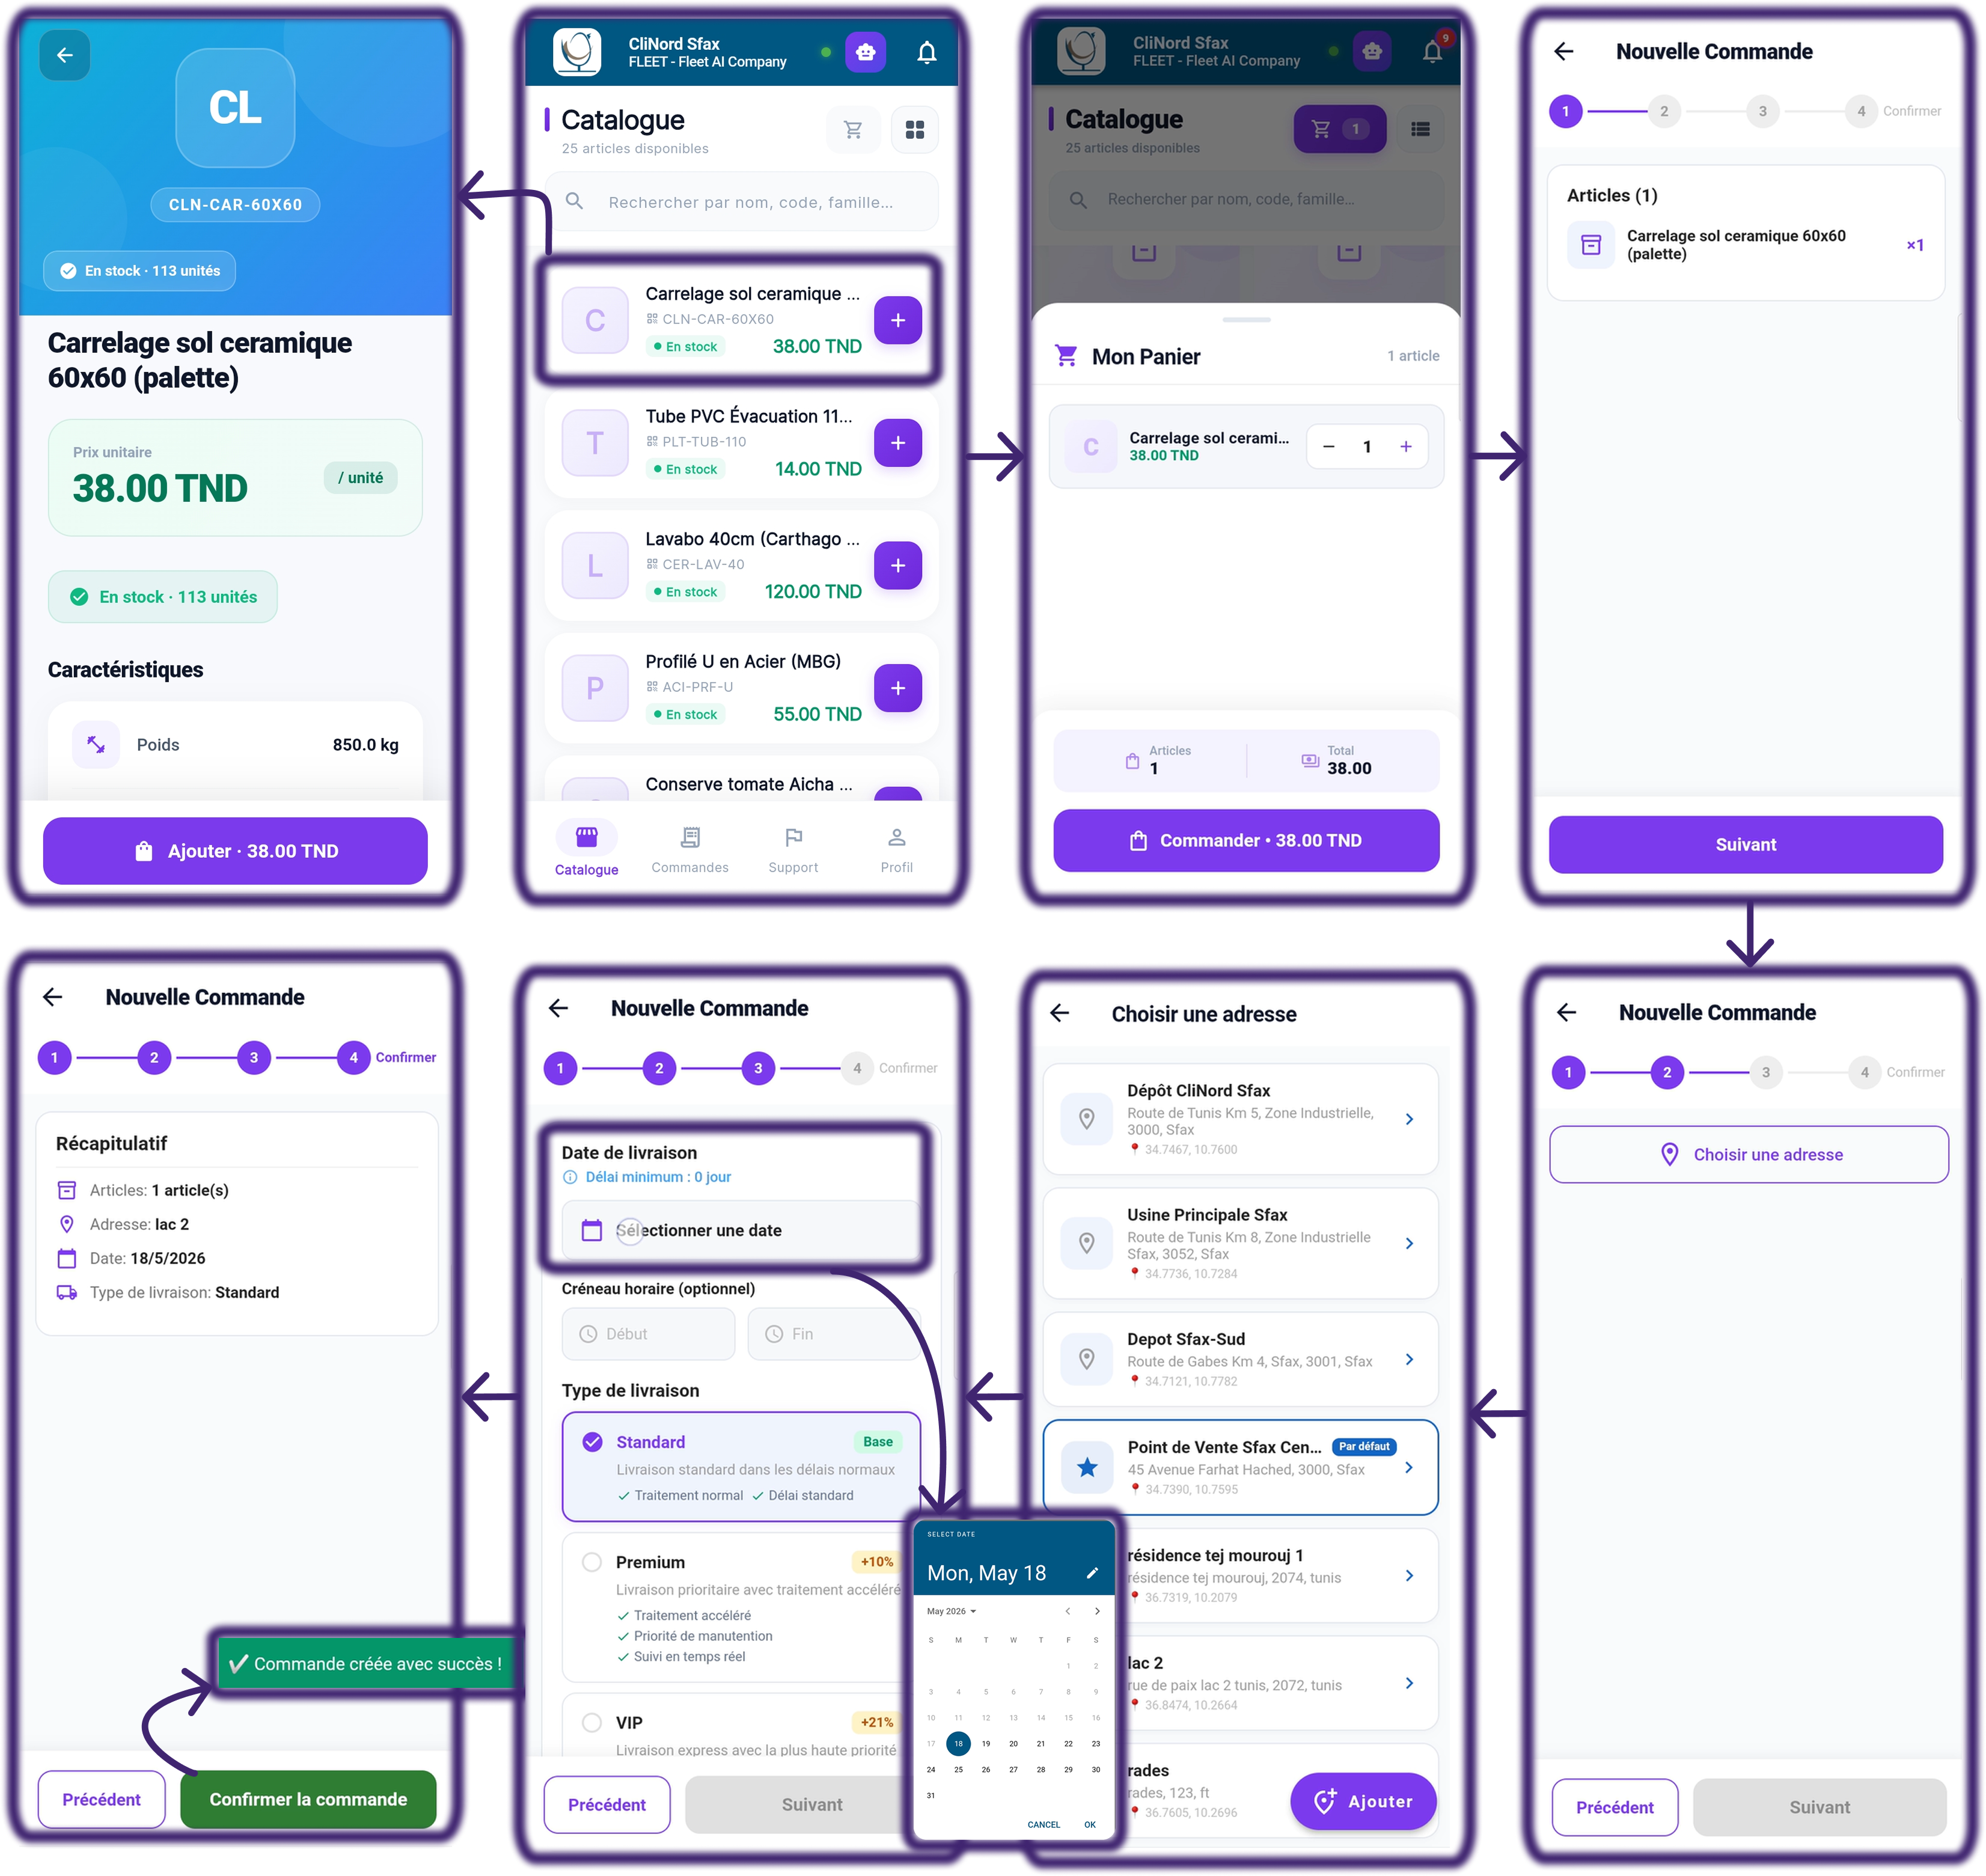
\includegraphics[width=\linewidth, height=0.40\textheight, keepaspectratio]{img/capture/mobile/realisation_commande_client}
\caption{Application mobile Client --- Processus complet de commande : catalogue, sélection d'article, panier, choix de l'adresse de livraison, type de livraison (Standard / Premium / VIP), sélection de créneau horaire et confirmation de la commande}
\label{fig:sp2-mobile-order}
\end{figure}

\begin{figure}[H]
\centering
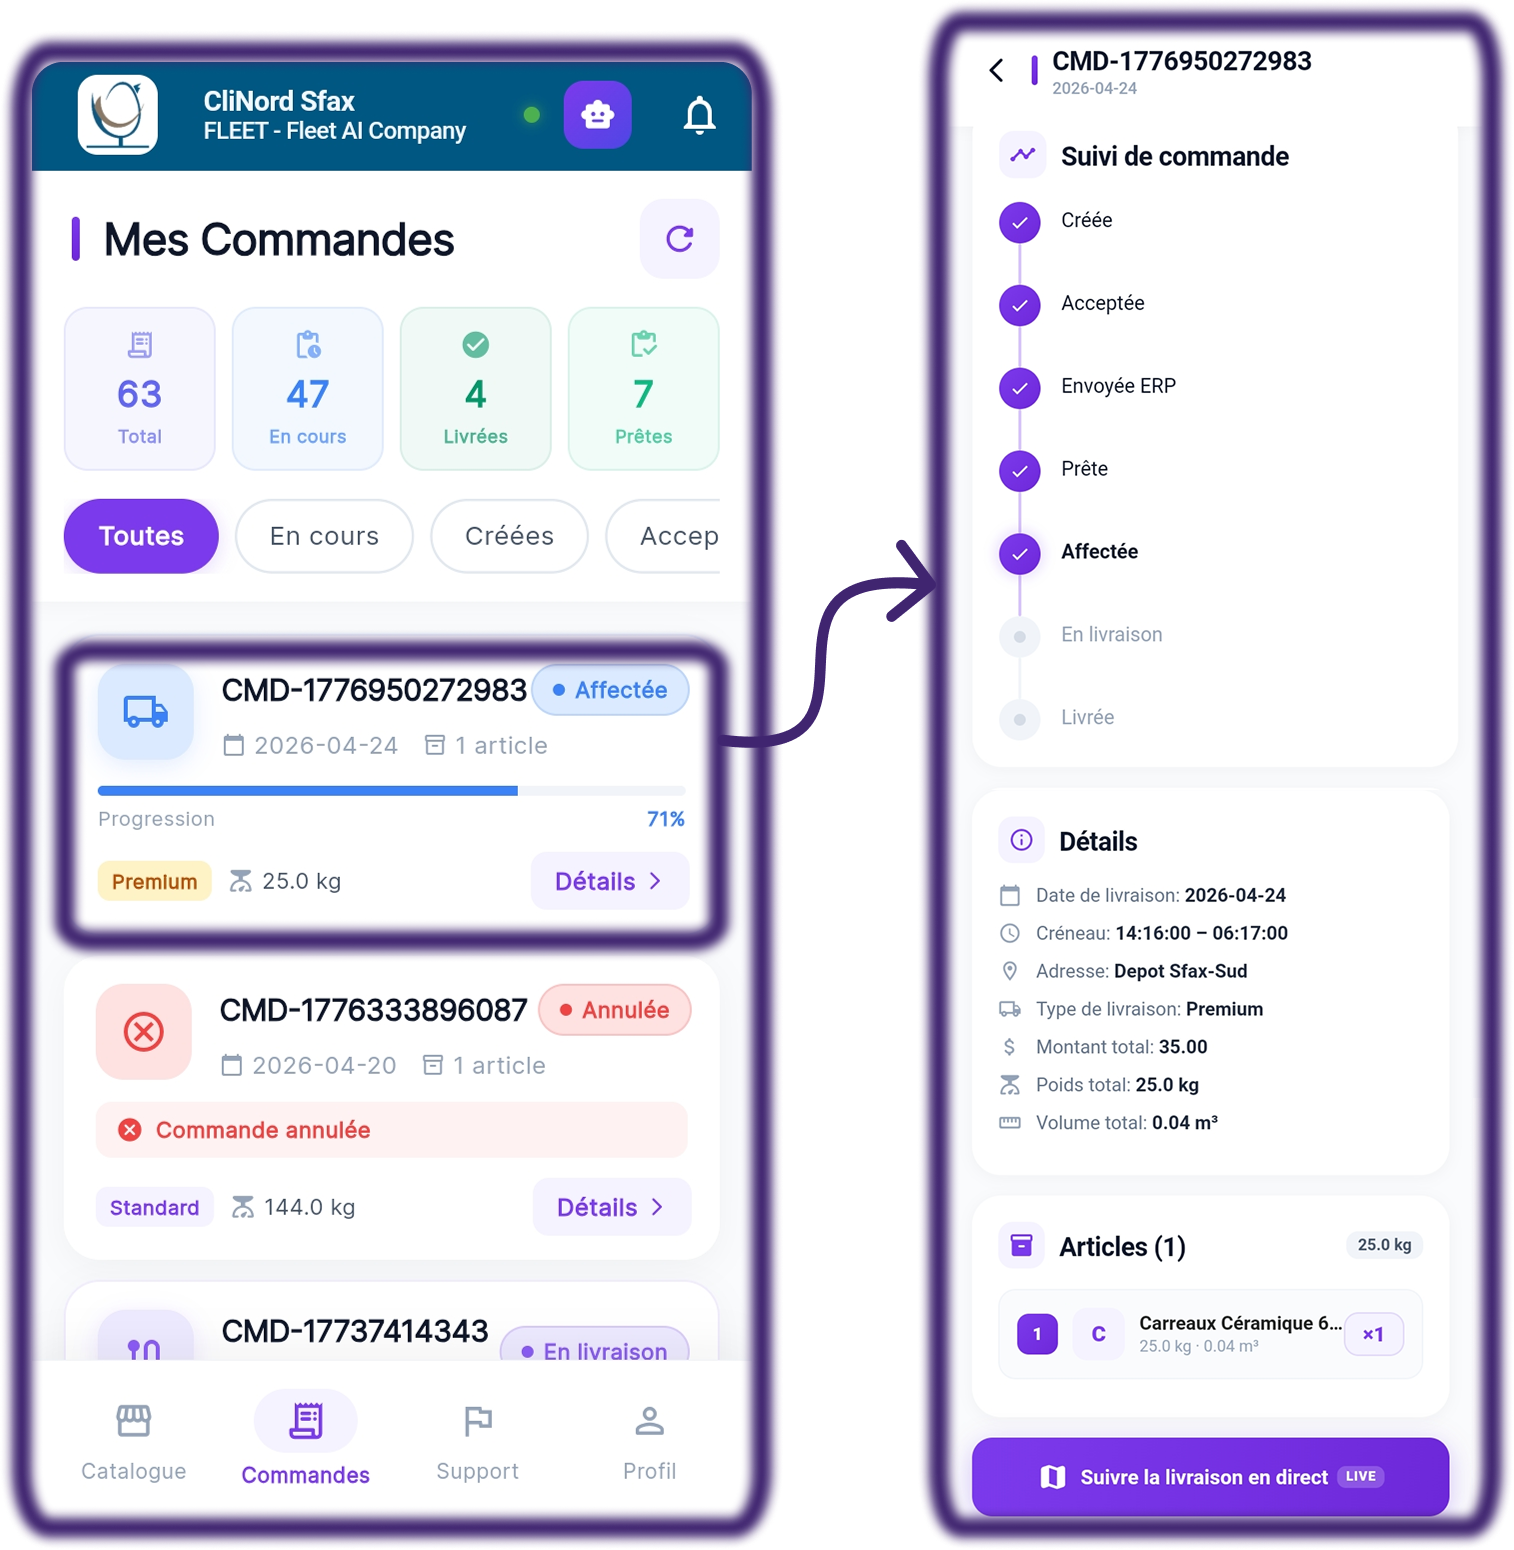
\includegraphics[width=0.55\linewidth, height=0.37\textheight, keepaspectratio]{img/capture/mobile/commande_client}
\caption{Application mobile Client --- Suivi des commandes : liste avec statuts (Affectée, En livraison, Annulée) et détail d'une commande avec progression live}
\label{fig:sp2-mobile-tracking}
\end{figure}

\subsection{Notifications du workflow client}

Le client est notifié automatiquement à chaque changement de statut de ses commandes (commande prête, mise en livraison, livraison échouée) depuis le centre de notifications de l'application mobile. Les notifications sont horodatées et classées par type ; le client peut consulter l'historique complet avec les compteurs (total, non lues, aujourd'hui).

\begin{figure}[H]
\centering
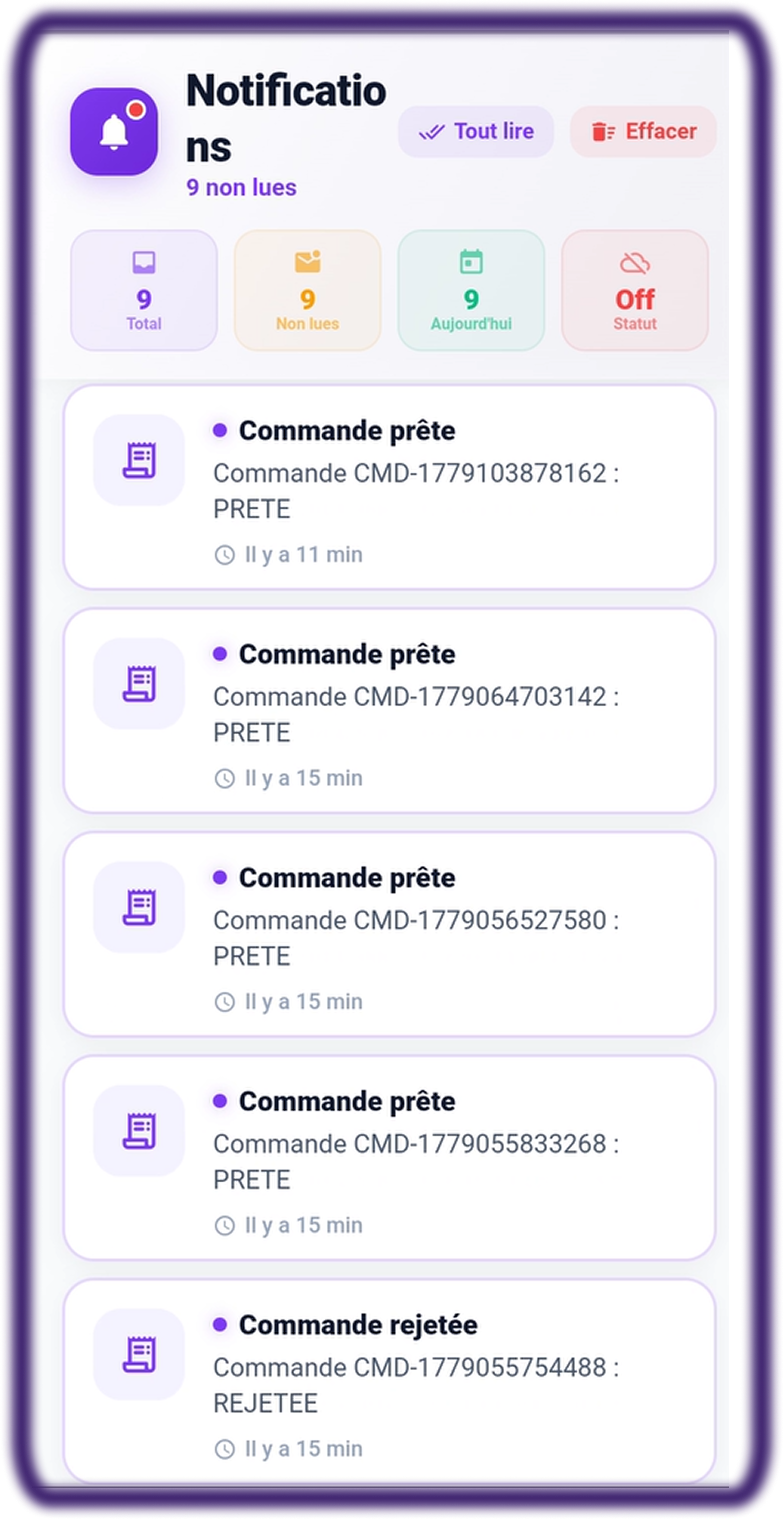
\includegraphics[width=0.40\linewidth, height=0.30\textheight, keepaspectratio]{img/capture/mobile/notification_client}
\caption{Application mobile Client --- Centre de notifications : alertes de statut de commande (prête, rejetée) avec horodatage et compteurs de lecture}
\label{fig:sp2-notification-client}
\end{figure}

\subsection{Profil client et gestion des adresses}

Le Client accède à son profil depuis l'onglet \textit{Profil}. Il y consulte le récapitulatif de ses commandes (total, actives, livrées, annulées) et gère ses adresses de livraison. L'ajout d'une adresse se fait soit manuellement (nom, adresse complète, code postal, ville), soit automatiquement via la géolocalisation GPS («~Utiliser ma position actuelle~»). Une adresse peut être marquée \textit{par défaut} pour être présélectionnée lors des commandes.

\begin{figure}[H]
\centering
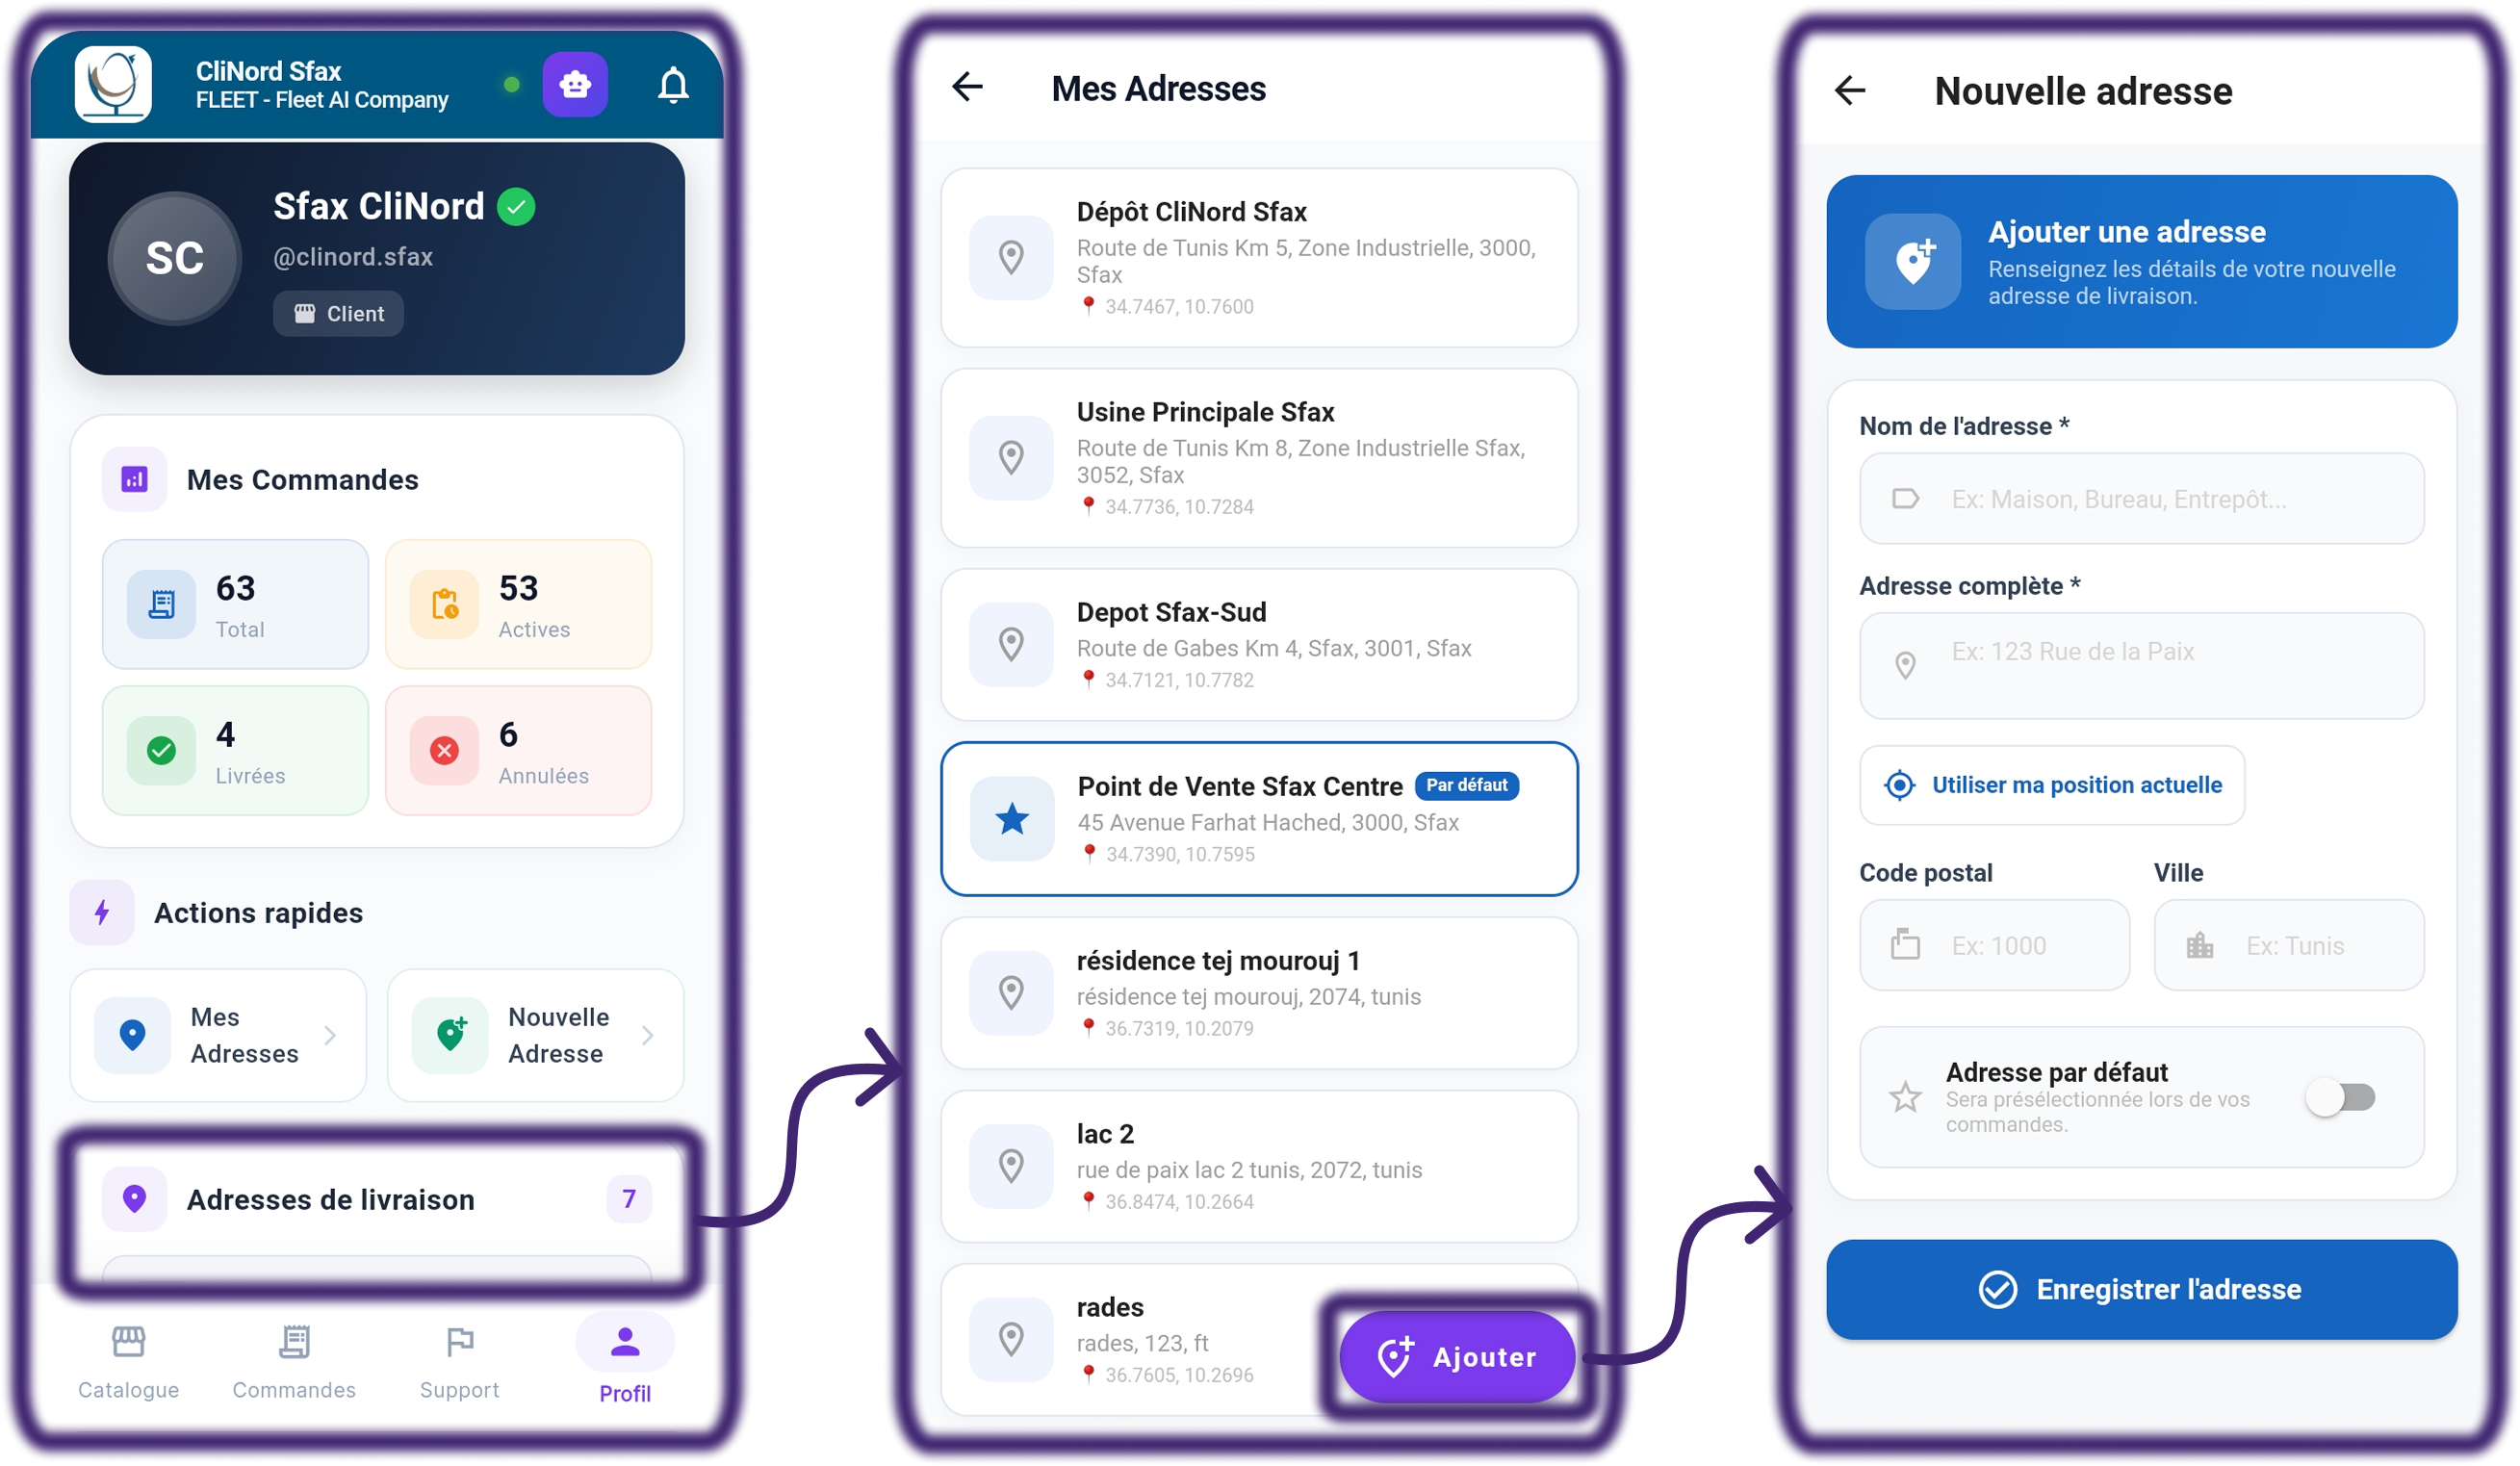
\includegraphics[width=\linewidth, height=0.38\textheight, keepaspectratio]{img/capture/mobile/profile_client}
\caption{Application mobile Client --- Profil et gestion des adresses : récapitulatif commandes, liste des adresses de livraison enregistrées et formulaire d'ajout d'une nouvelle adresse}
\label{fig:sp2-mobile-profile}
\end{figure}

% =============================================================
\section{Tests}
% =============================================================

\begin{figure}[H]
\centering
\IfFileExists{img/capture/web/sp2_test_e2e.png}{%
  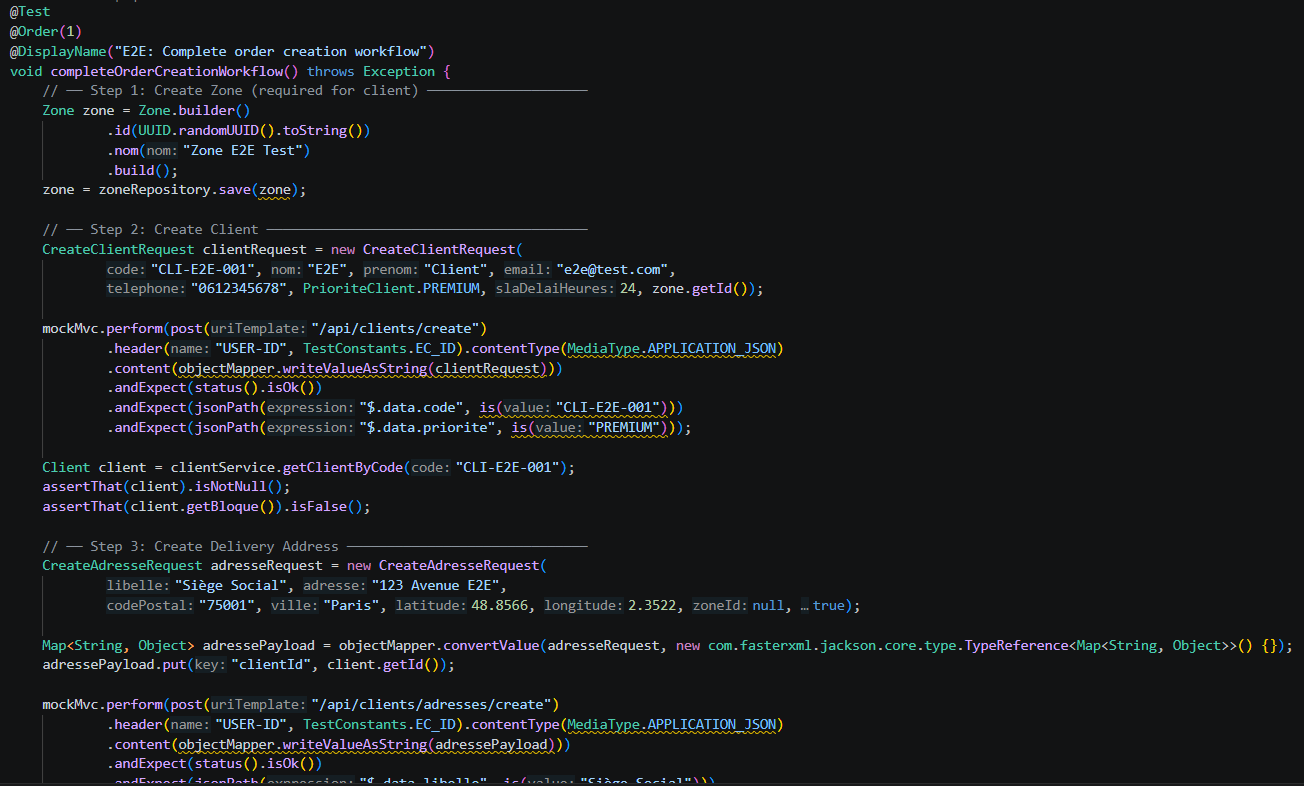
\includegraphics[width=\linewidth, keepaspectratio]{img/capture/web/sp2_test_e2e}%
}{%
  \fbox{\parbox{0.9\linewidth}{\centering\vspace{1.5cm}\textit{[img/capture/web/sp2\_test\_e2e.png]}\vspace{1.5cm}}}%
}
\caption{Exemple d'un test End-to-End (E2E) --- Sprint~2}
\label{fig:sp2-test}
\end{figure}

\begin{figure}[H]
\centering
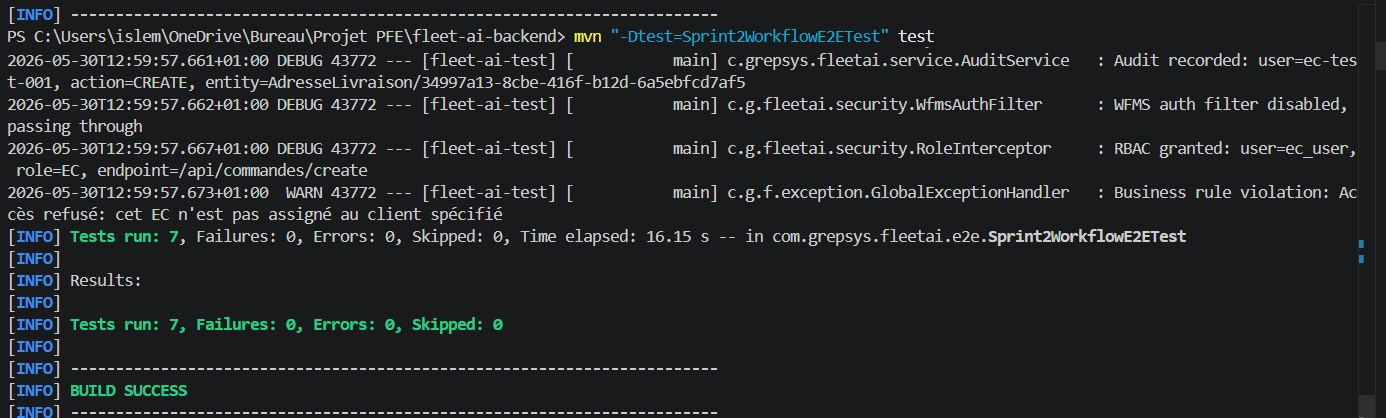
\includegraphics[width=\linewidth, height=0.32\textheight, keepaspectratio]{img/capture/web/sp2_resultat_test_e2e}
\caption{Résultats d'exécution des tests End-to-End --- Sprint~2 (Succès)}
\label{fig:sp2-test-result}
\end{figure}

\section*{Conclusion}
\addcontentsline{toc}{section}{Conclusion}

Le Sprint~2 livre le c{\oe}ur métier de Fleet~AI : gestion des clients, workflow de commandes à dix statuts, stock à deux niveaux et application mobile client. Le Sprint~3 couvre la planification et l'optimisation des tournées.


% ---- Chapitre 6 : Sprint 3 ----
\chapter{Sprint 3 : Planification \& Optimisation des Livraisons}

\section*{Introduction}
\addcontentsline{toc}{section}{Introduction}
Le Sprint~3 introduit le moteur de planification logistique de Fleet~AI. Il permet au Planificateur d'affecter les commandes prêtes aux chauffeurs disponibles, en tenant compte de la capacité des véhicules, des règles d'incompatibilité chauffeur-zone et de la charge journalière. Les plans de tournées journaliers et récurrents peuvent être créés, réordonnés et validés depuis l'interface web, avec génération des bons de chargement. Le Chauffeur consulte son itinéraire du jour et ses points de livraison depuis l'application mobile. Ce sprint marque la transition du référentiel vers l'opérationnel : les données des sprints précédents sont désormais mobilisées pour orchestrer les livraisons sur le terrain.

\section{Sprint Backlog}

\textbf{Objectif du sprint :} L'objectif est de rendre opérationnel le moteur de planification : affectation manuelle des commandes, création de plans journaliers et récurrents, génération des bons de chargement et consultation de l'itinéraire depuis l'application mobile Chauffeur.

\definecolor{headerbg}{HTML}{d5f5e3}
\setlength{\arrayrulewidth}{1pt}

Les story points (SP) sont estimés selon la suite de Fibonacci. L'échelle retenue est : 1--2 (tâche simple), 3--5 (complexité modérée), 8--13 (tâche complexe ou incertaine). Ce sprint totalise \textbf{20 stories, 99 SP}.

\begin{longtable}{|>{\raggedright\arraybackslash}p{4.2cm}|>{\raggedright\arraybackslash}p{4.8cm}|>{\raggedright\arraybackslash}p{4.5cm}|c|}
\hline
\rowcolor{headerbg}
\textbf{User Story} & \textbf{Tâche} & \textbf{Critères d'acceptation} & \textbf{\rotatebox{90}{SP}} \\
\hline
\endfirsthead
\hline
\rowcolor{headerbg}
\textbf{User Story} & \textbf{Tâche} & \textbf{Critères d'acceptation} & \textbf{\rotatebox{90}{SP}} \\
\hline
\endhead
\hline
\endfoot

%------ US-021 ------
\multirow{2}{=}{En tant que Planificateur, je veux assigner manuellement une commande à un chauffeur et un véhicule afin d'organiser les livraisons.}
& Vérifier la disponibilité du chauffeur et la capacité du véhicule avant de valider l'affectation. & L'affectation est bloquée si la capacité du véhicule est dépassée ou si le chauffeur est indisponible. & 3 \\
\cline{2-4}
& Permettre au Planificateur de sélectionner un chauffeur et un véhicule pour une commande avec indication des conflits. & Le formulaire signale clairement les conflits et bloque la soumission en cas d'incompatibilité. & 2 \\
\hline

%------ US-022 ------
\multirow{2}{=}{En tant que Planificateur, je veux créer un plan de livraison quotidien regroupant plusieurs commandes afin d'organiser la journée.}
& Permettre au Planificateur de regrouper plusieurs commandes dans un plan journalier avec calcul des distances estimées et de la charge par chauffeur. & Le plan affiche le nombre de commandes, les distances estimées et la charge par chauffeur. & 3 \\
\cline{2-4}
& Permettre au Planificateur de réordonner visuellement les commandes dans le plan journalier. & La liste des commandes du plan est réordonnée par le Planificateur avec mise à jour immédiate. & 2 \\
\hline

%------ US-023 ------
\multirow{2}{=}{En tant que Planificateur, je veux voir la charge de chaque chauffeur afin d'équilibrer les affectations.}
& Calculer et afficher la charge de chaque chauffeur (nombre de commandes, distances, poids) pour la journée en cours. & Un avertissement est affiché si un chauffeur dépasse le seuil de charge configuré. & 3 \\
\cline{2-4}
& Afficher un indicateur de surcharge par chauffeur dans le tableau de bord du Planificateur. & L'indicateur change de couleur si le chauffeur est surchargé ; visible directement sur le tableau de bord. & 2 \\
\hline

%------ US-024 ------
\multirow{2}{=}{En tant que Planificateur, je veux vérifier la capacité d'un véhicule avant affectation afin d'éviter les surcharges.}
& Vérifier automatiquement la capacité maximale (poids et volume) du véhicule à chaque tentative d'affectation. & L'affectation est bloquée si le poids ou le volume dépasse la capacité maximale du véhicule. & 3 \\
\cline{2-4}
& Afficher au Planificateur les indicateurs de capacité restante lors du formulaire d'affectation. & Les indicateurs de capacité poids/volume restante s'affichent et se mettent à jour en temps réel. & 2 \\
\hline

%------ US-025 ------
\multirow{2}{=}{En tant que Planificateur, je veux réassigner une livraison en cas de problème afin d'assurer la continuité du service.}
& Permettre au Planificateur de réassigner une livraison à un autre chauffeur disponible, avec notification au nouveau chauffeur. & La réassignation met à jour le plan et notifie le nouveau chauffeur automatiquement. & 3 \\
\cline{2-4}
& Afficher au Planificateur la liste des chauffeurs disponibles pour une réassignation depuis la fiche livraison. & La fenêtre de réassignation s'affiche depuis la fiche livraison ; la liste des disponibles est filtrée. & 2 \\
\hline

%------ US-026 ------
\multirow{2}{=}{En tant que Planificateur, je veux que le système estime les distances entre les points de livraison afin d'optimiser les itinéraires.}
& Calculer les distances entre les points de livraison à partir des coordonnées géographiques enregistrées. & Les distances sont calculées et affichées ; la précision est acceptable pour les zones urbaines tunisiennes. & 5 \\
\cline{2-4}
& Valider les calculs de distance sur des jeux de données représentatifs de zones réelles. & Les distances calculées sont cohérentes avec les distances réelles sur les itinéraires utilisés. & 3 \\
\hline

%------ US-027 ------
\multirow{2}{=}{En tant que Planificateur, je veux gérer les créneaux horaires de livraison demandés par les clients afin de respecter leurs contraintes.}
& Intégrer les créneaux horaires demandés dans le modèle de commande et les vérifier lors de l'affectation. & Les créneaux sont respectés lors de l'affectation ; un conflit de créneau est signalé au Planificateur. & 2 \\
\cline{2-4}
& Permettre au REC de saisir un créneau horaire lors de la création ou modification d'une commande. & Le sélecteur de créneau est disponible dans le formulaire ; les conflits sont affichés avant soumission. & 1 \\
\hline

%------ US-028 ------
\multirow{2}{=}{En tant que Planificateur, je veux créer des plans de livraison hebdomadaires récurrents afin de gagner du temps.}
& Permettre au Planificateur de définir un modèle de plan hebdomadaire récurrent avec sélection des jours. & Le plan récurrent se génère automatiquement chaque semaine à partir du modèle défini. & 3 \\
\cline{2-4}
& Permettre au Planificateur d'activer ou désactiver un plan récurrent depuis son tableau de bord. & Le modèle de plan récurrent est sauvegardé et peut être activé ou désactivé. & 2 \\
\hline

%------ US-029 ------
\multirow{2}{=}{En tant que Planificateur, je veux générer un bon de chargement pour l'entrepôt afin de faciliter la préparation des expéditions.}
& Générer un document de chargement listant les articles par commande et par véhicule, sous format téléchargeable. & Le document liste les articles par commande et par véhicule ; téléchargeable en un clic. & 3 \\
\cline{2-4}
& Mettre à disposition du Planificateur le bouton de génération du bon de chargement depuis la page du plan journalier. & Le document est généré et téléchargeable depuis l'interface en un clic. & 2 \\
\hline

%------ US-030 ------
\multirow{2}{=}{En tant que Planificateur, je veux reprogrammer les livraisons échouées au jour suivant afin de finaliser les commandes.}
& Proposer automatiquement les livraisons échouées en priorité dans le plan du lendemain. & Les livraisons échouées sont proposées en priorité dans le plan du lendemain. & 3 \\
\cline{2-4}
& Afficher au Planificateur un panneau dédié aux livraisons à reprogrammer avec option de validation rapide. & Le panneau des livraisons à reprogrammer s'affiche avec option de validation rapide. & 2 \\
\hline

%------ US-031 ------
\multirow{2}{=}{En tant que Planificateur, je veux définir des règles d'incompatibilité entre chauffeurs et zones afin d'éviter les erreurs d'attribution.}
& Permettre au Planificateur de définir des règles d'incompatibilité entre un chauffeur et une zone, vérifiées à chaque affectation. & La règle est vérifiée lors de chaque affectation ; une alerte est levée en cas de violation. & 2 \\
\cline{2-4}
& Permettre au Planificateur de consulter et modifier la liste des règles d'incompatibilité définies. & La liste des règles est consultable et modifiable ; les violations sont signalées lors de l'affectation. & 1 \\
\hline

%------ US-032 ------
\multirow{2}{=}{En tant que Planificateur, je veux recevoir des suggestions d'itinéraires optimisés afin de minimiser les kilomètres parcourus.}
& Générer des itinéraires optimisés tenant compte de la capacité des véhicules, des créneaux horaires et des zones de livraison. & Le système produit des itinéraires optimisés ; le gain en kilomètres est calculé et affiché. & 8 \\
\cline{2-4}
& Afficher les suggestions d'itinéraires dans le tableau de bord du Planificateur avec un indicateur de qualité. & Les suggestions s'affichent dans le tableau de bord avec un score de qualité. & 5 \\
\hline

%------ US-033 ------
\multirow{2}{=}{En tant que Planificateur, je veux accepter, modifier ou rejeter chaque suggestion d'itinéraire afin de garder le contrôle sur les décisions.}
& Permettre au Planificateur de valider, ajuster ou rejeter chaque suggestion avec traçabilité pour améliorer les suggestions futures. & Le Planificateur peut valider, éditer ou rejeter ; l'action est enregistrée pour la rétroaction. & 3 \\
\cline{2-4}
& Mettre à disposition les actions (Accepter / Modifier / Rejeter) pour chaque suggestion avec possibilité d'ajustement. & Les actions sont accessibles sur chaque suggestion ; un formulaire d'ajustement est disponible. & 2 \\
\hline

%------ US-037 ------
\multirow{2}{=}{En tant que Planificateur, je veux recevoir des suggestions du chauffeur le plus adapté afin d'optimiser les affectations.}
& Calculer un score de pertinence pour chaque chauffeur selon ses performances, sa zone et sa disponibilité, et proposer les 3 meilleurs candidats. & Le système propose les 3 chauffeurs les plus adaptés avec un score de pertinence et une justification. & 3 \\
\cline{2-4}
& Afficher les suggestions de chauffeurs avec score et justification dans le formulaire d'affectation. & Les 3 suggestions s'affichent avec score et justification (zone, performance, disponibilité). & 2 \\
\hline

%------ US-034 ------
\multirow{2}{=}{En tant que Chauffeur, je veux voir l'itinéraire optimisé sur une carte afin de faciliter mes déplacements.}
& Afficher au Chauffeur les points de livraison numérotés dans l'ordre optimal sur une carte. & La carte affiche les points de livraison numérotés dans l'ordre optimal de passage. & 3 \\
\cline{2-4}
& Permettre au Chauffeur de lancer la navigation vers chaque point de livraison depuis l'application mobile. & Le Chauffeur peut lancer la navigation vers chaque point depuis l'application mobile. & 2 \\
\hline

%------ US-035 ------
\multirow{2}{=}{En tant que Planificateur, je veux que le système respecte toutes les contraintes métier lors de l'optimisation afin de garantir la faisabilité des suggestions.}
& Intégrer les contraintes métier dans le moteur d'optimisation (capacité, créneaux, zones, règles d'incompatibilité). & Aucune suggestion ne viole les contraintes définies ; un rapport de faisabilité est fourni. & 5 \\
\cline{2-4}
& Présenter au Planificateur un rapport des contraintes respectées et des éventuelles violations pour chaque suggestion. & Le rapport de faisabilité est consultable depuis l'interface de validation des suggestions. & 3 \\
\hline

%------ US-036 ------
\multirow{2}{=}{En tant que Planificateur, je veux que les parties prenantes soient notifiées après validation du plan afin d'assurer la coordination entre acteurs.}
& Envoyer une notification adaptée à chaque destinataire (Chauffeur, REC, Client) après validation du plan. & Le Chauffeur, le Responsable et le Client reçoivent chacun une notification adaptée à leur rôle. & 3 \\
\cline{2-4}
& Délivrer les notifications dans les 30 secondes suivant la validation du plan. & Les notifications apparaissent dans les 30 secondes suivant la validation. & 2 \\
\hline

%------ US-038 ------
\multirow{2}{=}{En tant que Planificateur, je veux envoyer des retours au système afin d'améliorer la qualité des suggestions futures.}
& Permettre au Planificateur d'enregistrer un retour (acceptation ou rejet avec motif) sur chaque suggestion du système. & Les retours sont enregistrés et utilisés pour améliorer les suggestions futures. & 3 \\
\cline{2-4}
& Afficher un formulaire de retour au Planificateur après chaque rejet d'une suggestion. & Le formulaire de motif est affiché après chaque rejet ; la saisie est optionnelle mais encouragée. & 2 \\
\hline

%------ US-106 ------
\multirow{2}{=}{En tant que Planificateur, je veux un tableau de bord opérationnel en temps réel afin de suivre l'avancement des livraisons.}
& Exposer au Planificateur les métriques opérationnelles en temps réel (livraisons en cours, retards, alertes). & Le tableau de bord s'actualise régulièrement ; les retards et alertes s'affichent automatiquement. & 3 \\
\cline{2-4}
& Afficher les indicateurs opérationnels (livraisons en cours, retards détectés, alertes) dans le tableau de bord. & Les indicateurs s'affichent avec mise à jour automatique. & 2 \\
\hline

%------ US-131 ------
\multirow{2}{=}{En tant que Chauffeur, je veux voir mes livraisons du jour et l'itinéraire optimisé sur la carte depuis l'application mobile.}
& Récupérer et afficher au Chauffeur la liste de ses livraisons du jour, triées dans l'ordre optimal défini par le Planificateur. & La liste des livraisons du jour est récupérée et triée dans l'ordre optimal défini par le Planificateur. & 3 \\
\cline{2-4}
& Afficher la carte avec les points de livraison numérotés et permettre la navigation vers chaque point. & La carte s'affiche avec les points numérotés ; la navigation est accessible pour chaque point. & 2 \\
\hline

\caption{Sprint Backlog du Sprint 3 --- Planification \& Optimisation (20 stories, 99 SP)}
\end{longtable}
\setlength{\arrayrulewidth}{0.4pt}


% =============================================================
\section{Conception}
% =============================================================

\subsection{Diagramme de cas d'utilisation}

\begin{figure}[H]
\centering
\IfFileExists{img/diagrammes/sprint_3_usecase_p1.png}{%
  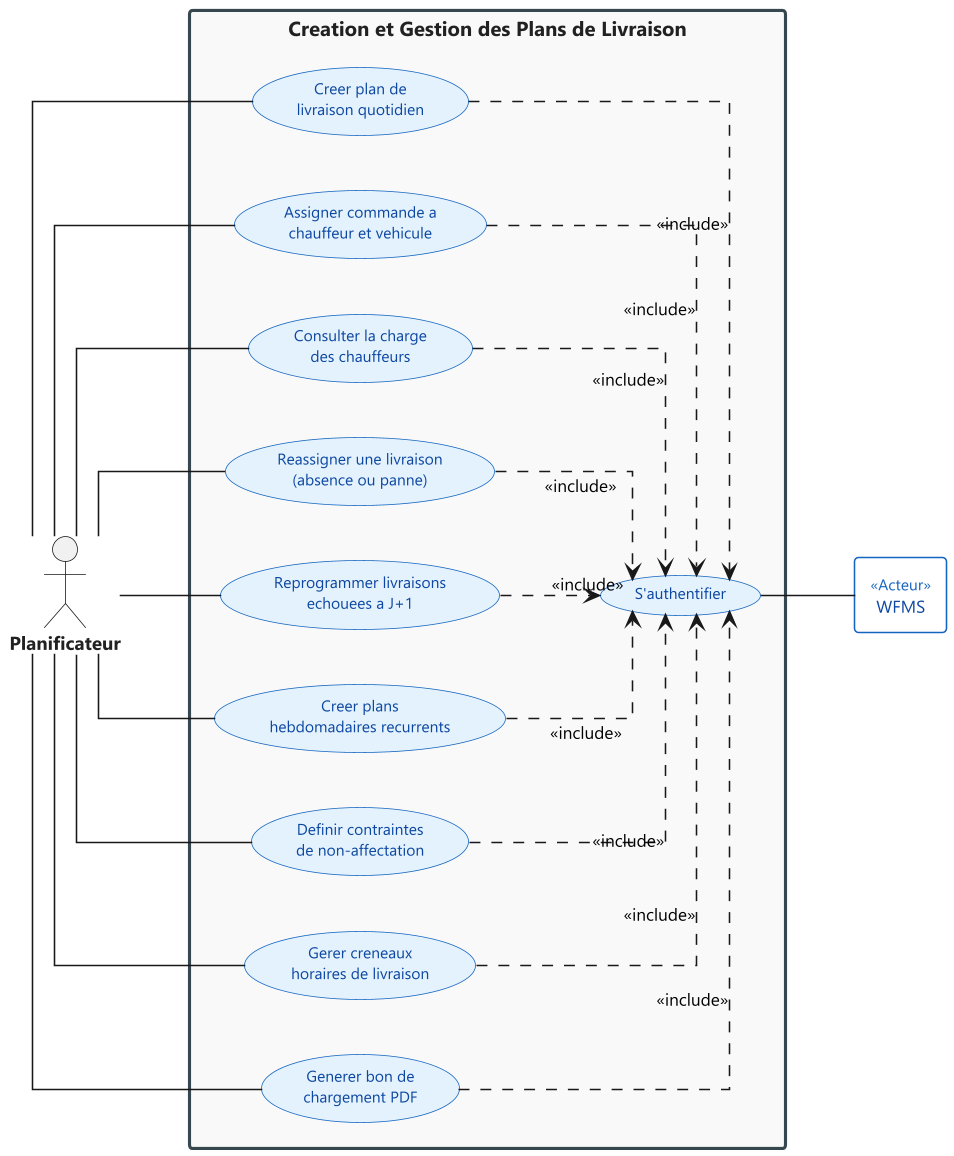
\includegraphics[width=0.9\textwidth, height=0.85\textheight, keepaspectratio]{img/diagrammes/sprint_3_usecase_p1}%
}{%
  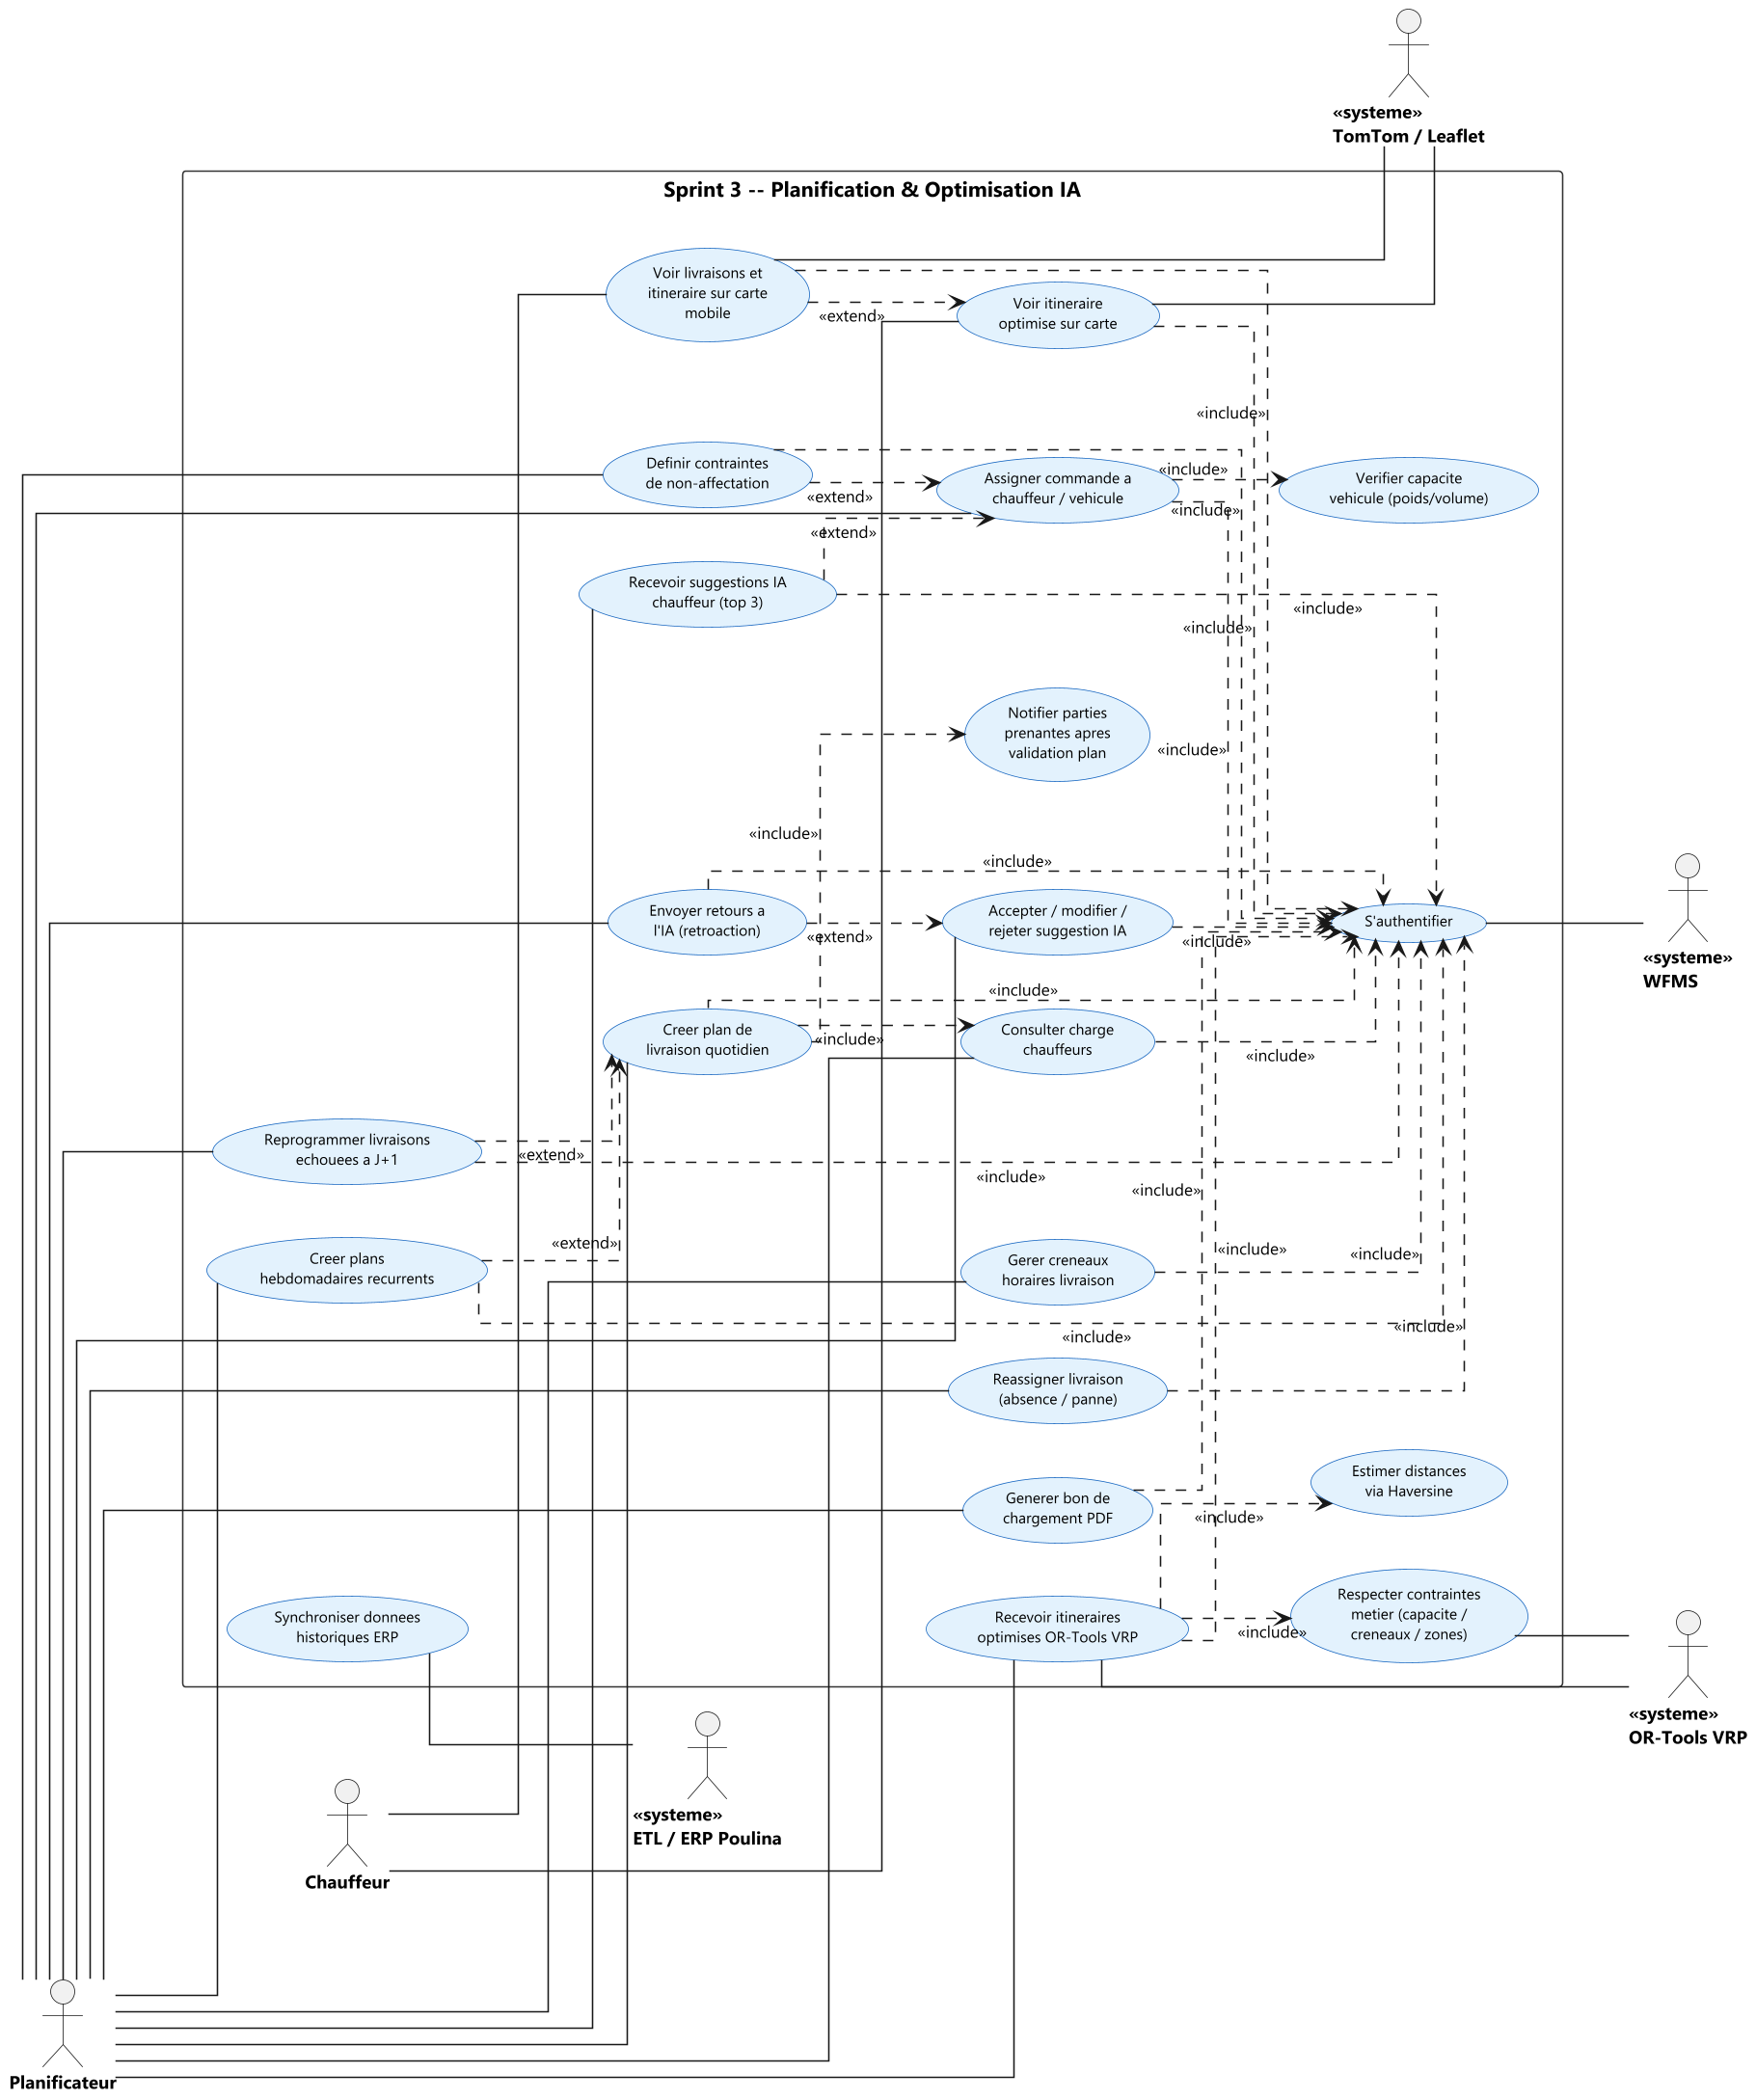
\includegraphics[width=0.9\textwidth, height=0.85\textheight, keepaspectratio]{img/diagrammes/sprint_3_usecase}%
}
\caption{Diagramme de cas d'utilisation du Sprint~3 --- Partie~1}
\label{fig:cas-utilisation-sp3-p1}
\end{figure}

\begin{figure}[H]
\centering
\IfFileExists{img/diagrammes/sprint_3_usecase_p2.png}{%
  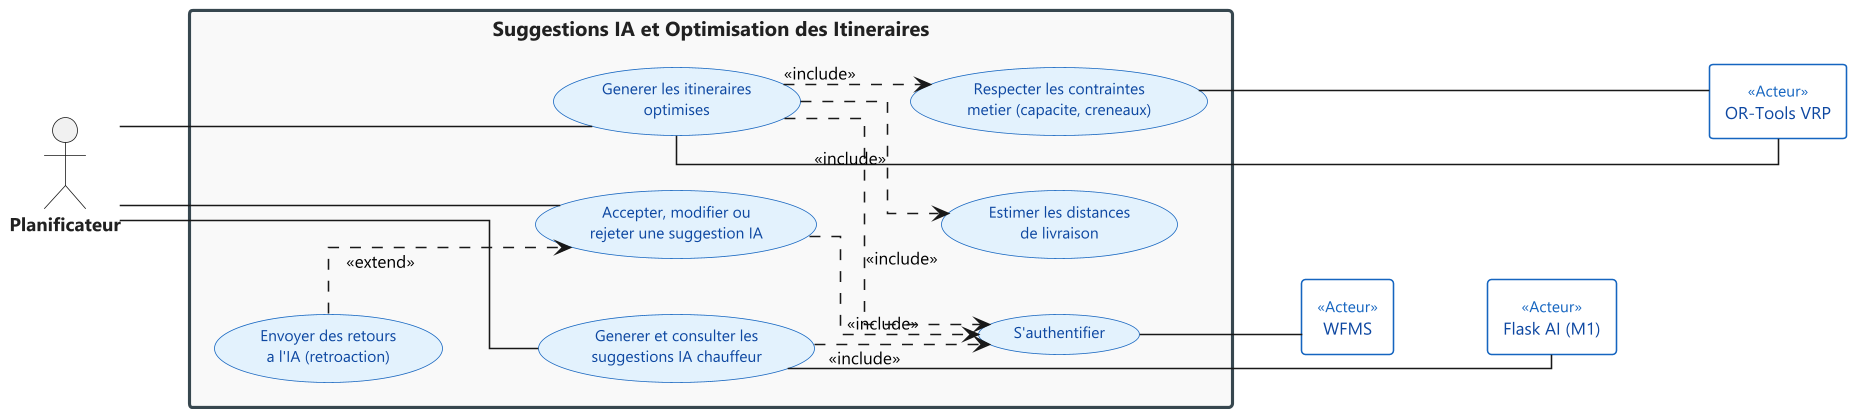
\includegraphics[width=0.9\textwidth, height=0.85\textheight, keepaspectratio]{img/diagrammes/sprint_3_usecase_p2}%
}{%
  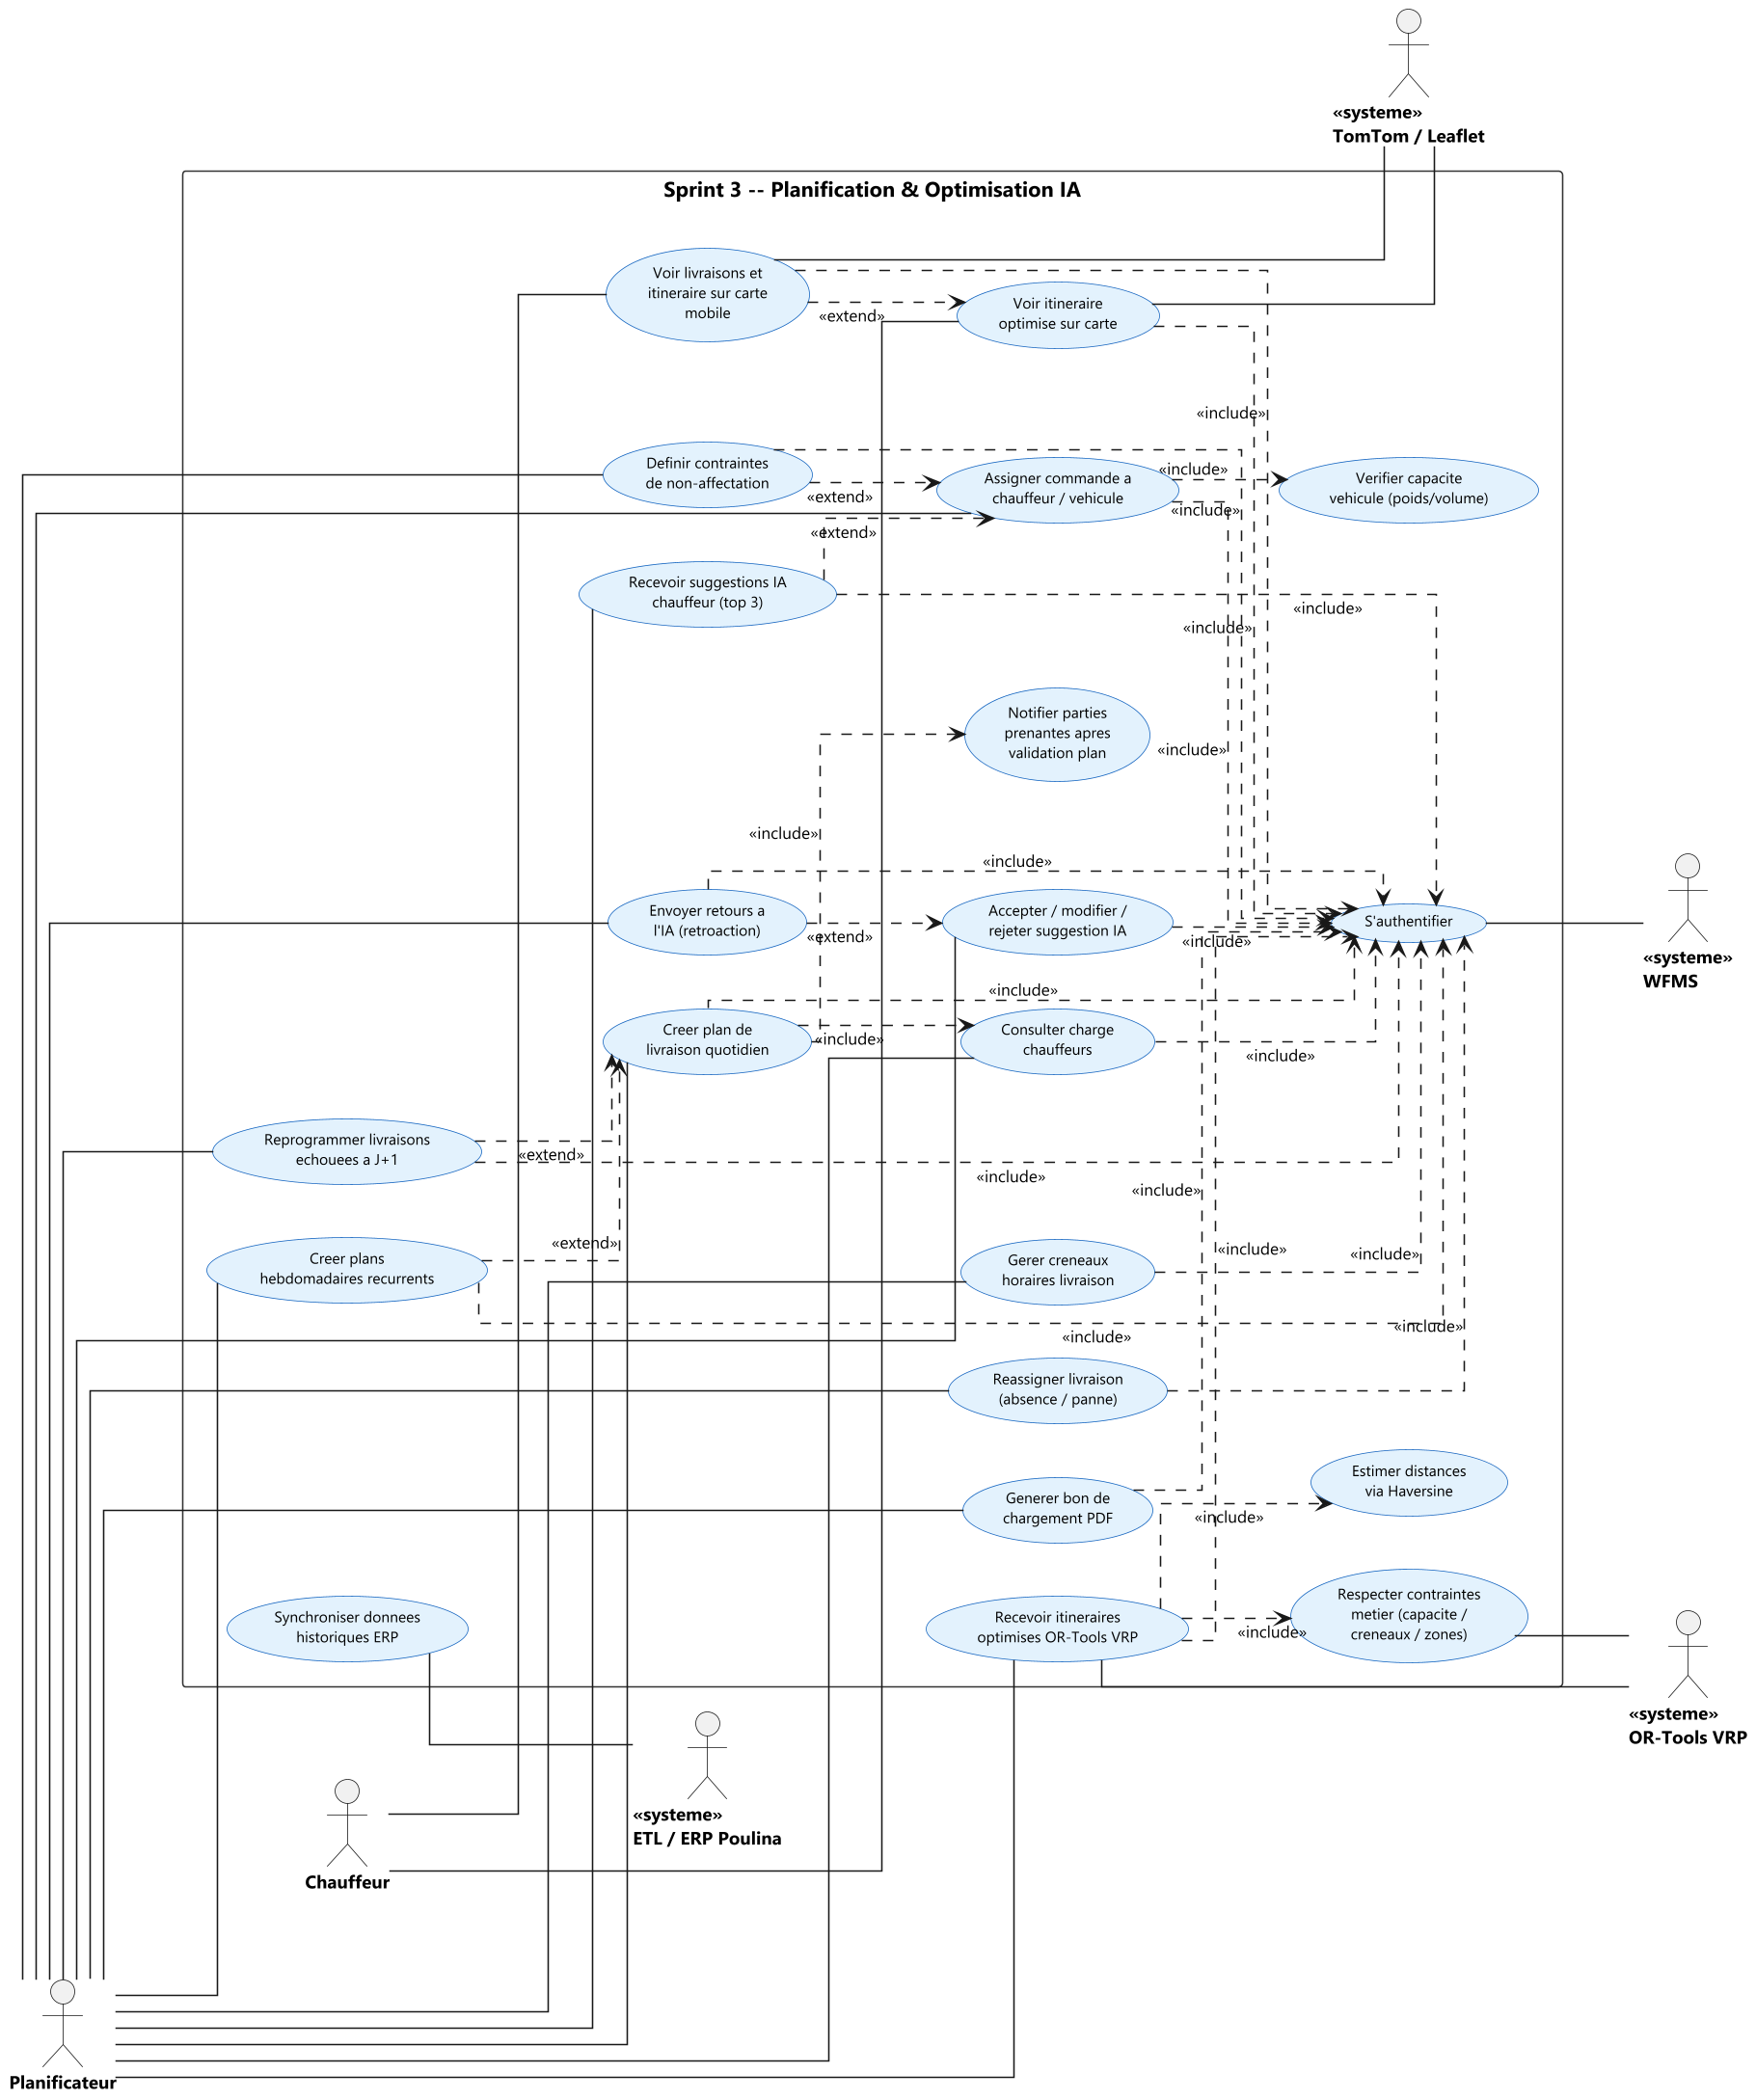
\includegraphics[width=0.9\textwidth, height=0.85\textheight, keepaspectratio]{img/diagrammes/sprint_3_usecase}%
}
\caption{Diagramme de cas d'utilisation du Sprint~3 --- Partie~2}
\label{fig:cas-utilisation-sp3-p2}
\end{figure}

\begin{figure}[H]
\centering
\IfFileExists{img/diagrammes/sprint_3_usecase_p3.png}{%
  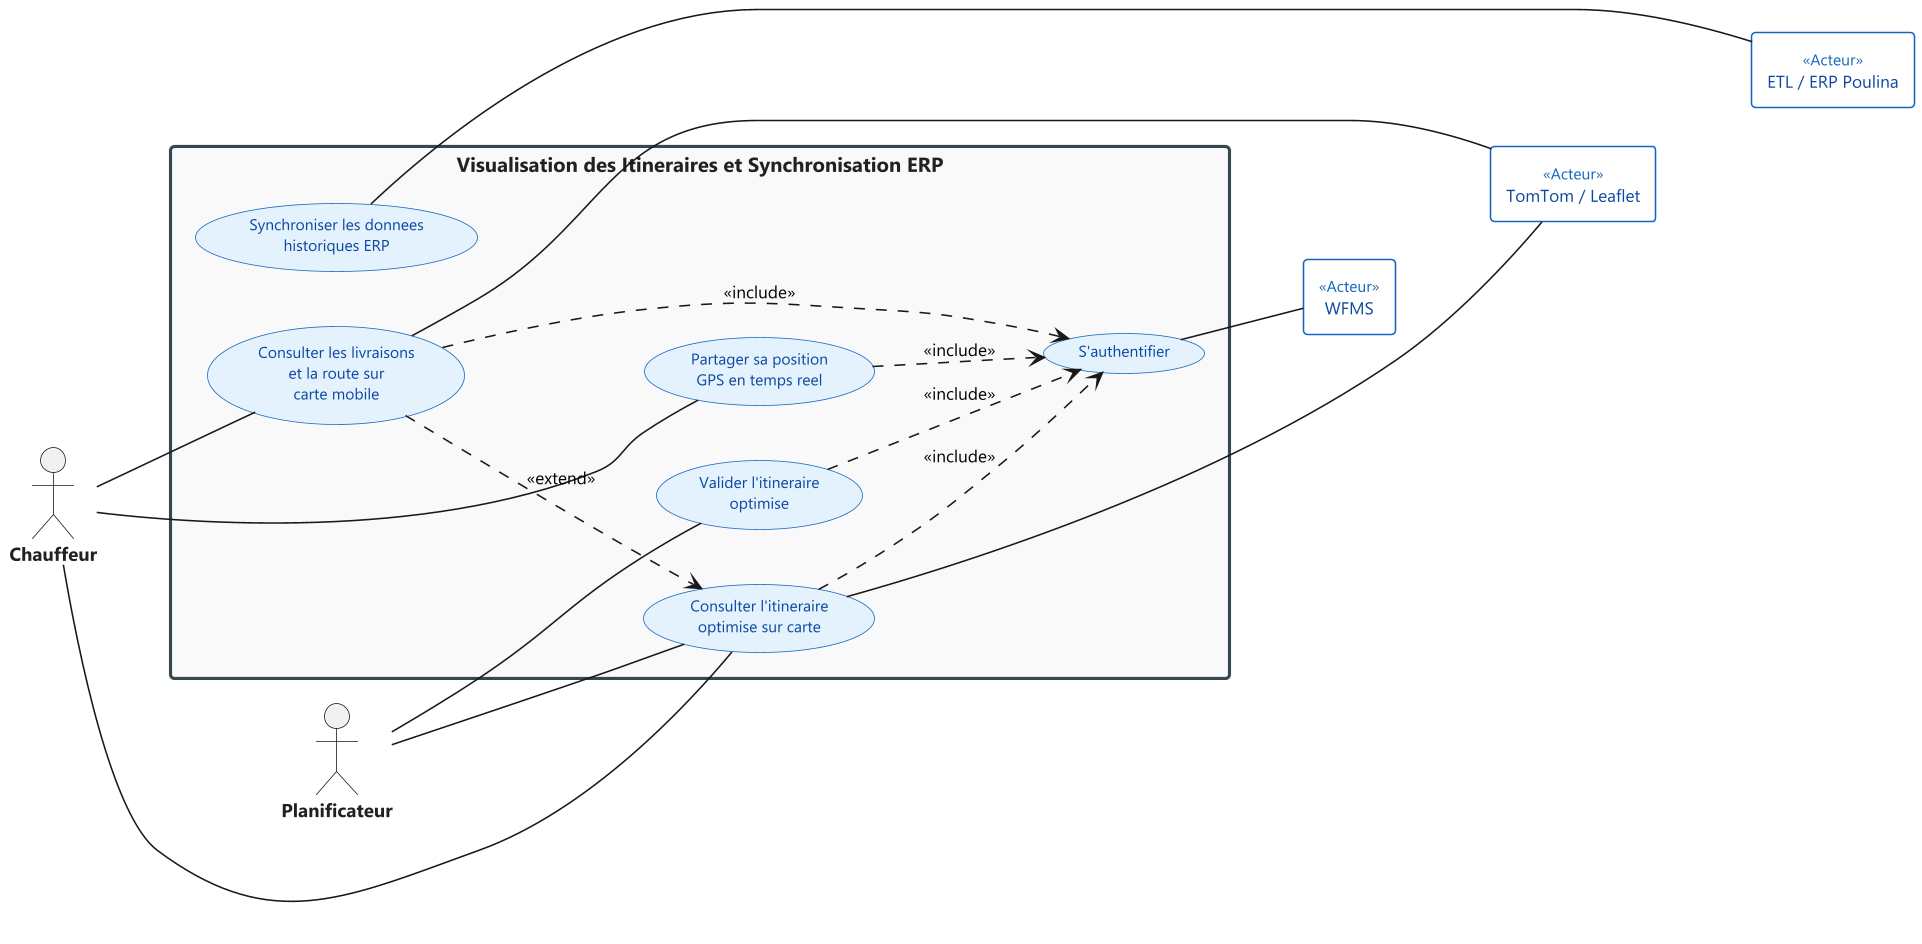
\includegraphics[width=0.9\textwidth, height=0.85\textheight, keepaspectratio]{img/diagrammes/sprint_3_usecase_p3}%
}{%
  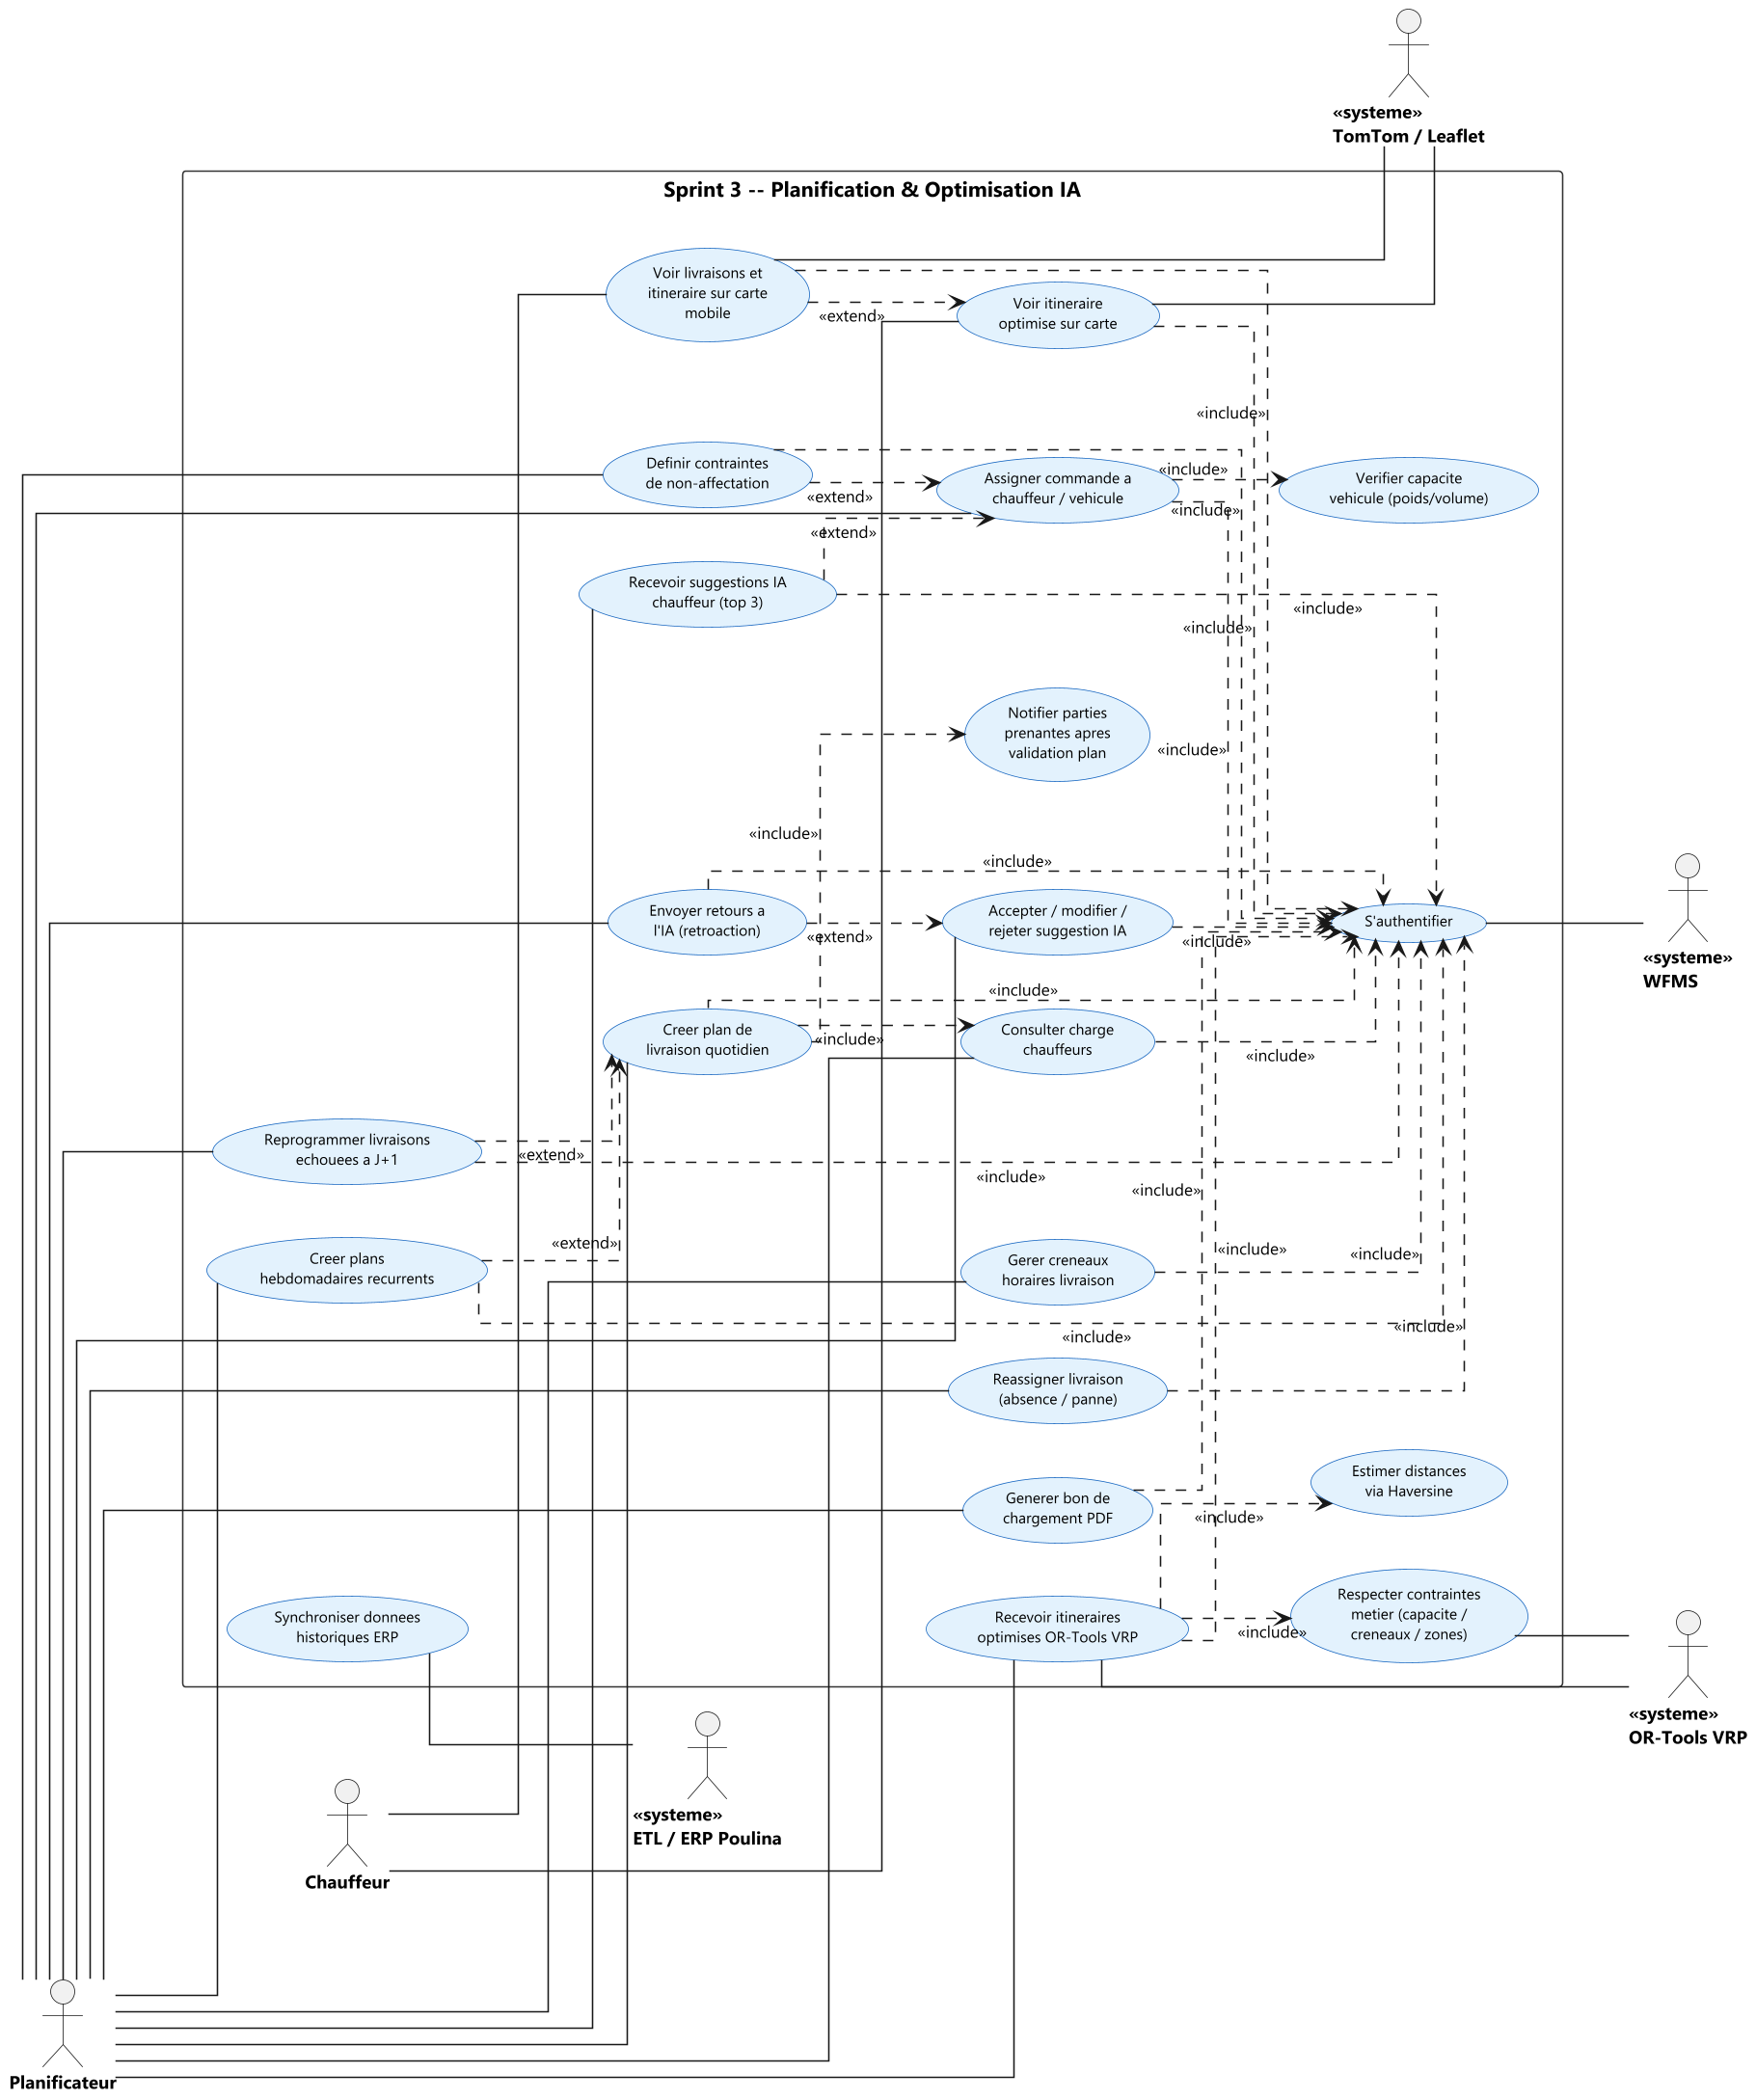
\includegraphics[width=0.9\textwidth, height=0.85\textheight, keepaspectratio]{img/diagrammes/sprint_3_usecase}%
}
\caption{Diagramme de cas d'utilisation du Sprint~3 --- Partie~3}
\label{fig:cas-utilisation-sp3-p3}
\end{figure}

\subsection{Description textuelle}

Le diagramme de cas d'utilisation du Sprint~3 implique deux acteurs métier principaux --- le \textbf{Planificateur} et le \textbf{Chauffeur} --- ainsi que trois systèmes externes : \textbf{WFMS} (authentification), \textbf{ETL / ERP Poulina} (synchronisation des données historiques) et \textbf{OR-Tools VRP} (moteur d'optimisation d'itinéraires). La carte est rendue via \textbf{TomTom / Leaflet}.

\captionsetup[longtable]{justification=centering}
\setlength{\arrayrulewidth}{1pt}
\begin{longtable}{|p{4cm}|p{11cm}|}
\hline
\rowcolor{headerbg}
\textbf{Élément} & \textbf{Description} \\
\hline
\textbf{Titre} & Planification et gestion des tournées \\
\hline
\textbf{Acteurs} & Planificateur, Chauffeur, ETL / ERP Poulina, TomTom / Leaflet \\
\hline
\textbf{Objectif} & Permettre au Planificateur de créer des plans de livraison journaliers et récurrents, de gérer la charge des chauffeurs, de contrôler les capacités véhicules et de générer les bons de chargement. \\
\hline
\textbf{Précondition} & Les commandes sont au statut PRÊTE. Le Planificateur est authentifié via WFMS. Les données historiques ERP sont synchronisées. \\
\hline
\textbf{Postcondition} & Le plan est validé, les commandes passent à AFFECTÉE et les parties prenantes (Chauffeur, REC, Client) sont notifiées. \\
\hline
\textbf{Scénario nominal} &
\begin{enumerate}[start=1, label=\arabic*., nosep, leftmargin=1.4em]
    \item Le Planificateur s'authentifie via WFMS et accède à l'interface de planification.
    \item Il crée un plan de livraison quotidien en sélectionnant les commandes prêtes.
    \item Il consulte la charge des chauffeurs disponibles et assigne commandes/véhicules.
    \item Le système vérifie la capacité du véhicule (poids et volume) à chaque affectation.
    \item Le Planificateur consulte la charge et la capacité restante de chaque chauffeur et véhicule ; les indicateurs de surcharge s'affichent en temps réel.
    \item Il définit les règles d'incompatibilité chauffeur-zone et configure des plans récurrents hebdomadaires.
    \item Après validation, le bon de chargement PDF est généré et les parties prenantes sont notifiées.
    \item Le Chauffeur consulte ses livraisons du jour et son itinéraire sur la carte mobile (TomTom / Leaflet).
\end{enumerate} \\
\hline
\textbf{Scénario alternatif} &
\begin{enumerate}[start=1, label=\arabic*., nosep, leftmargin=1.4em]
    \item Aucun chauffeur disponible : le Planificateur peut définir des contraintes de non-affectation ou reprogrammer les livraisons échouées à J+1.
    \item Capacité véhicule dépassée : l'affectation est bloquée avec message explicite.
    \item Règle d'incompatibilité chauffeur-zone : une alerte est levée ; l'affectation est refusée.
    \item Livraison échouée : le Planificateur la reprogramme en priorité le lendemain.
\end{enumerate} \\
\hline
\caption{Description textuelle --- Planification et gestion des tournées (Sprint 3)}
\end{longtable}
\setlength{\arrayrulewidth}{0.4pt}

\subsection{Diagramme de classes}

\newpage
\thispagestyle{empty}
\begin{landscape}
\begin{figure}[H]
\centering
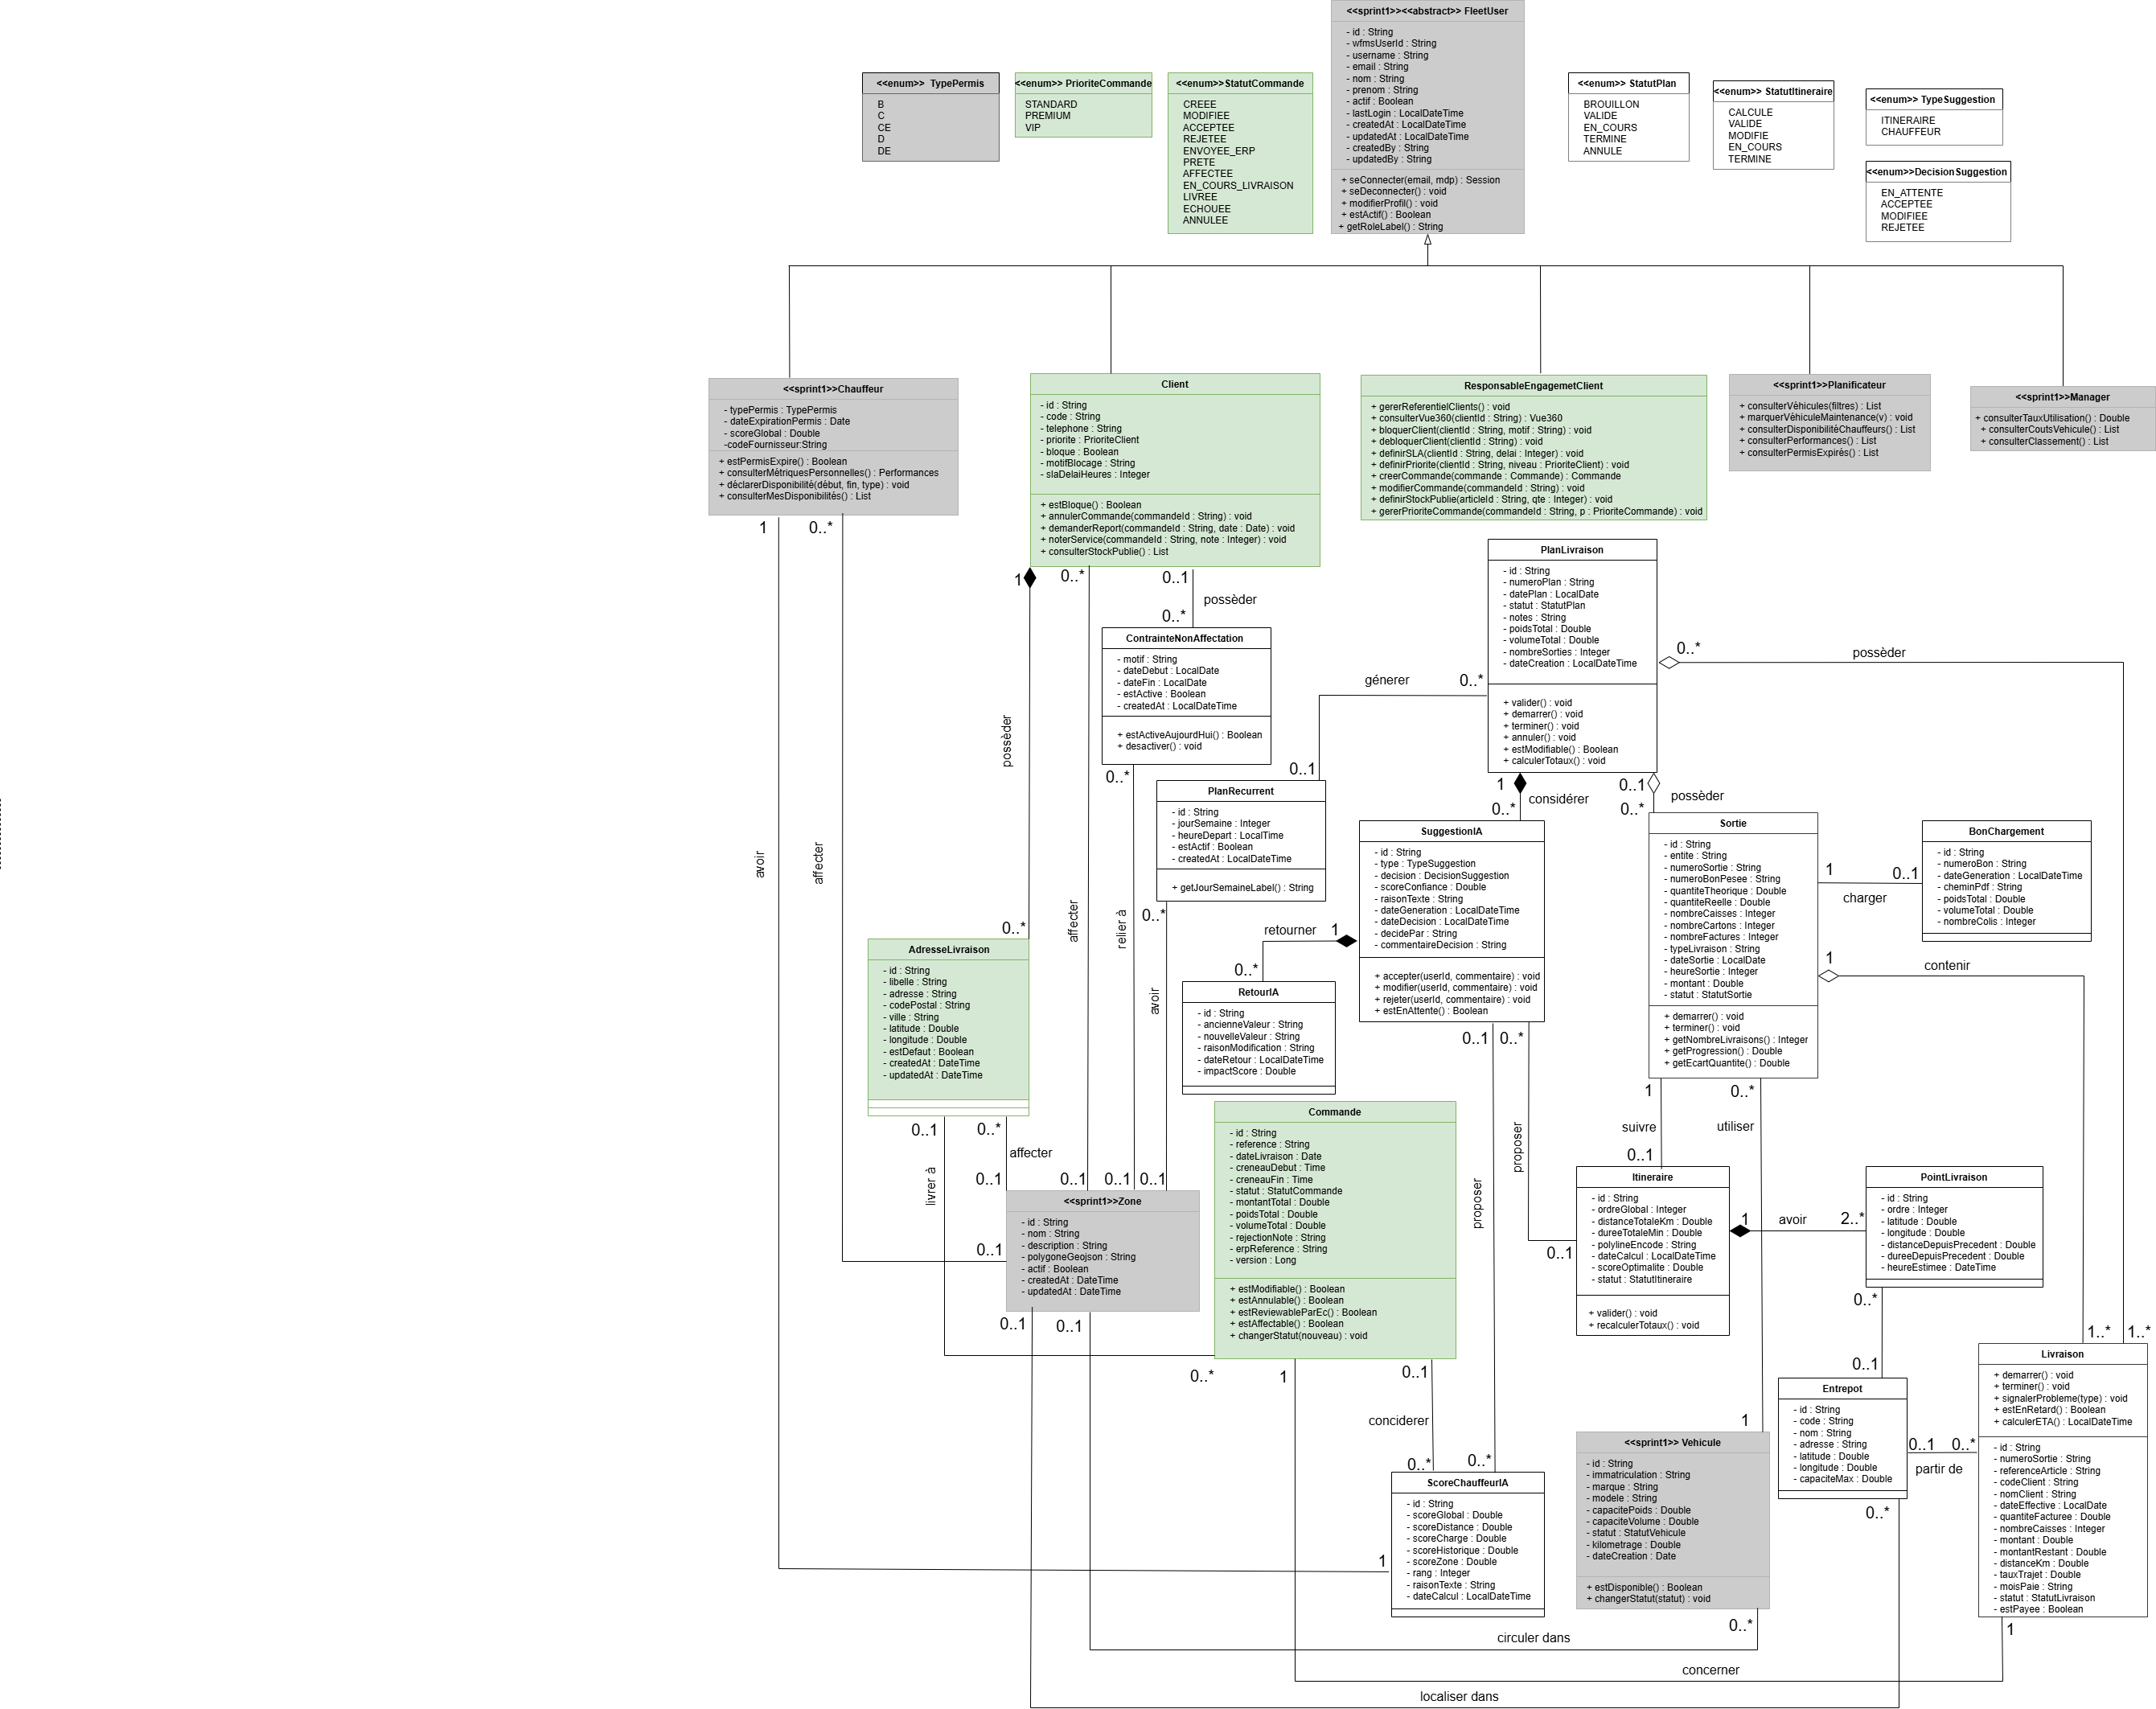
\includegraphics[width=\linewidth, height=0.95\textheight, keepaspectratio]{img/diagrammes/sprint_3_classes}
\caption{Diagramme de classes du Sprint 3}
\label{fig:diag-classes-sp3}
\end{figure}
\end{landscape}

% =============================================================
\section{Réalisation}
% =============================================================

\subsection{Affectation manuelle et gestion de la charge}

Le Planificateur sélectionne les commandes au statut PRÊTE et les affecte à un chauffeur et un véhicule disponibles. Le système vérifie en temps réel la disponibilité, la capacité restante et les règles d'incompatibilité chauffeur-zone.

\begin{figure}[H]
\centering
\IfFileExists{img/capture/web/sp3_planning_composite.png}{%
  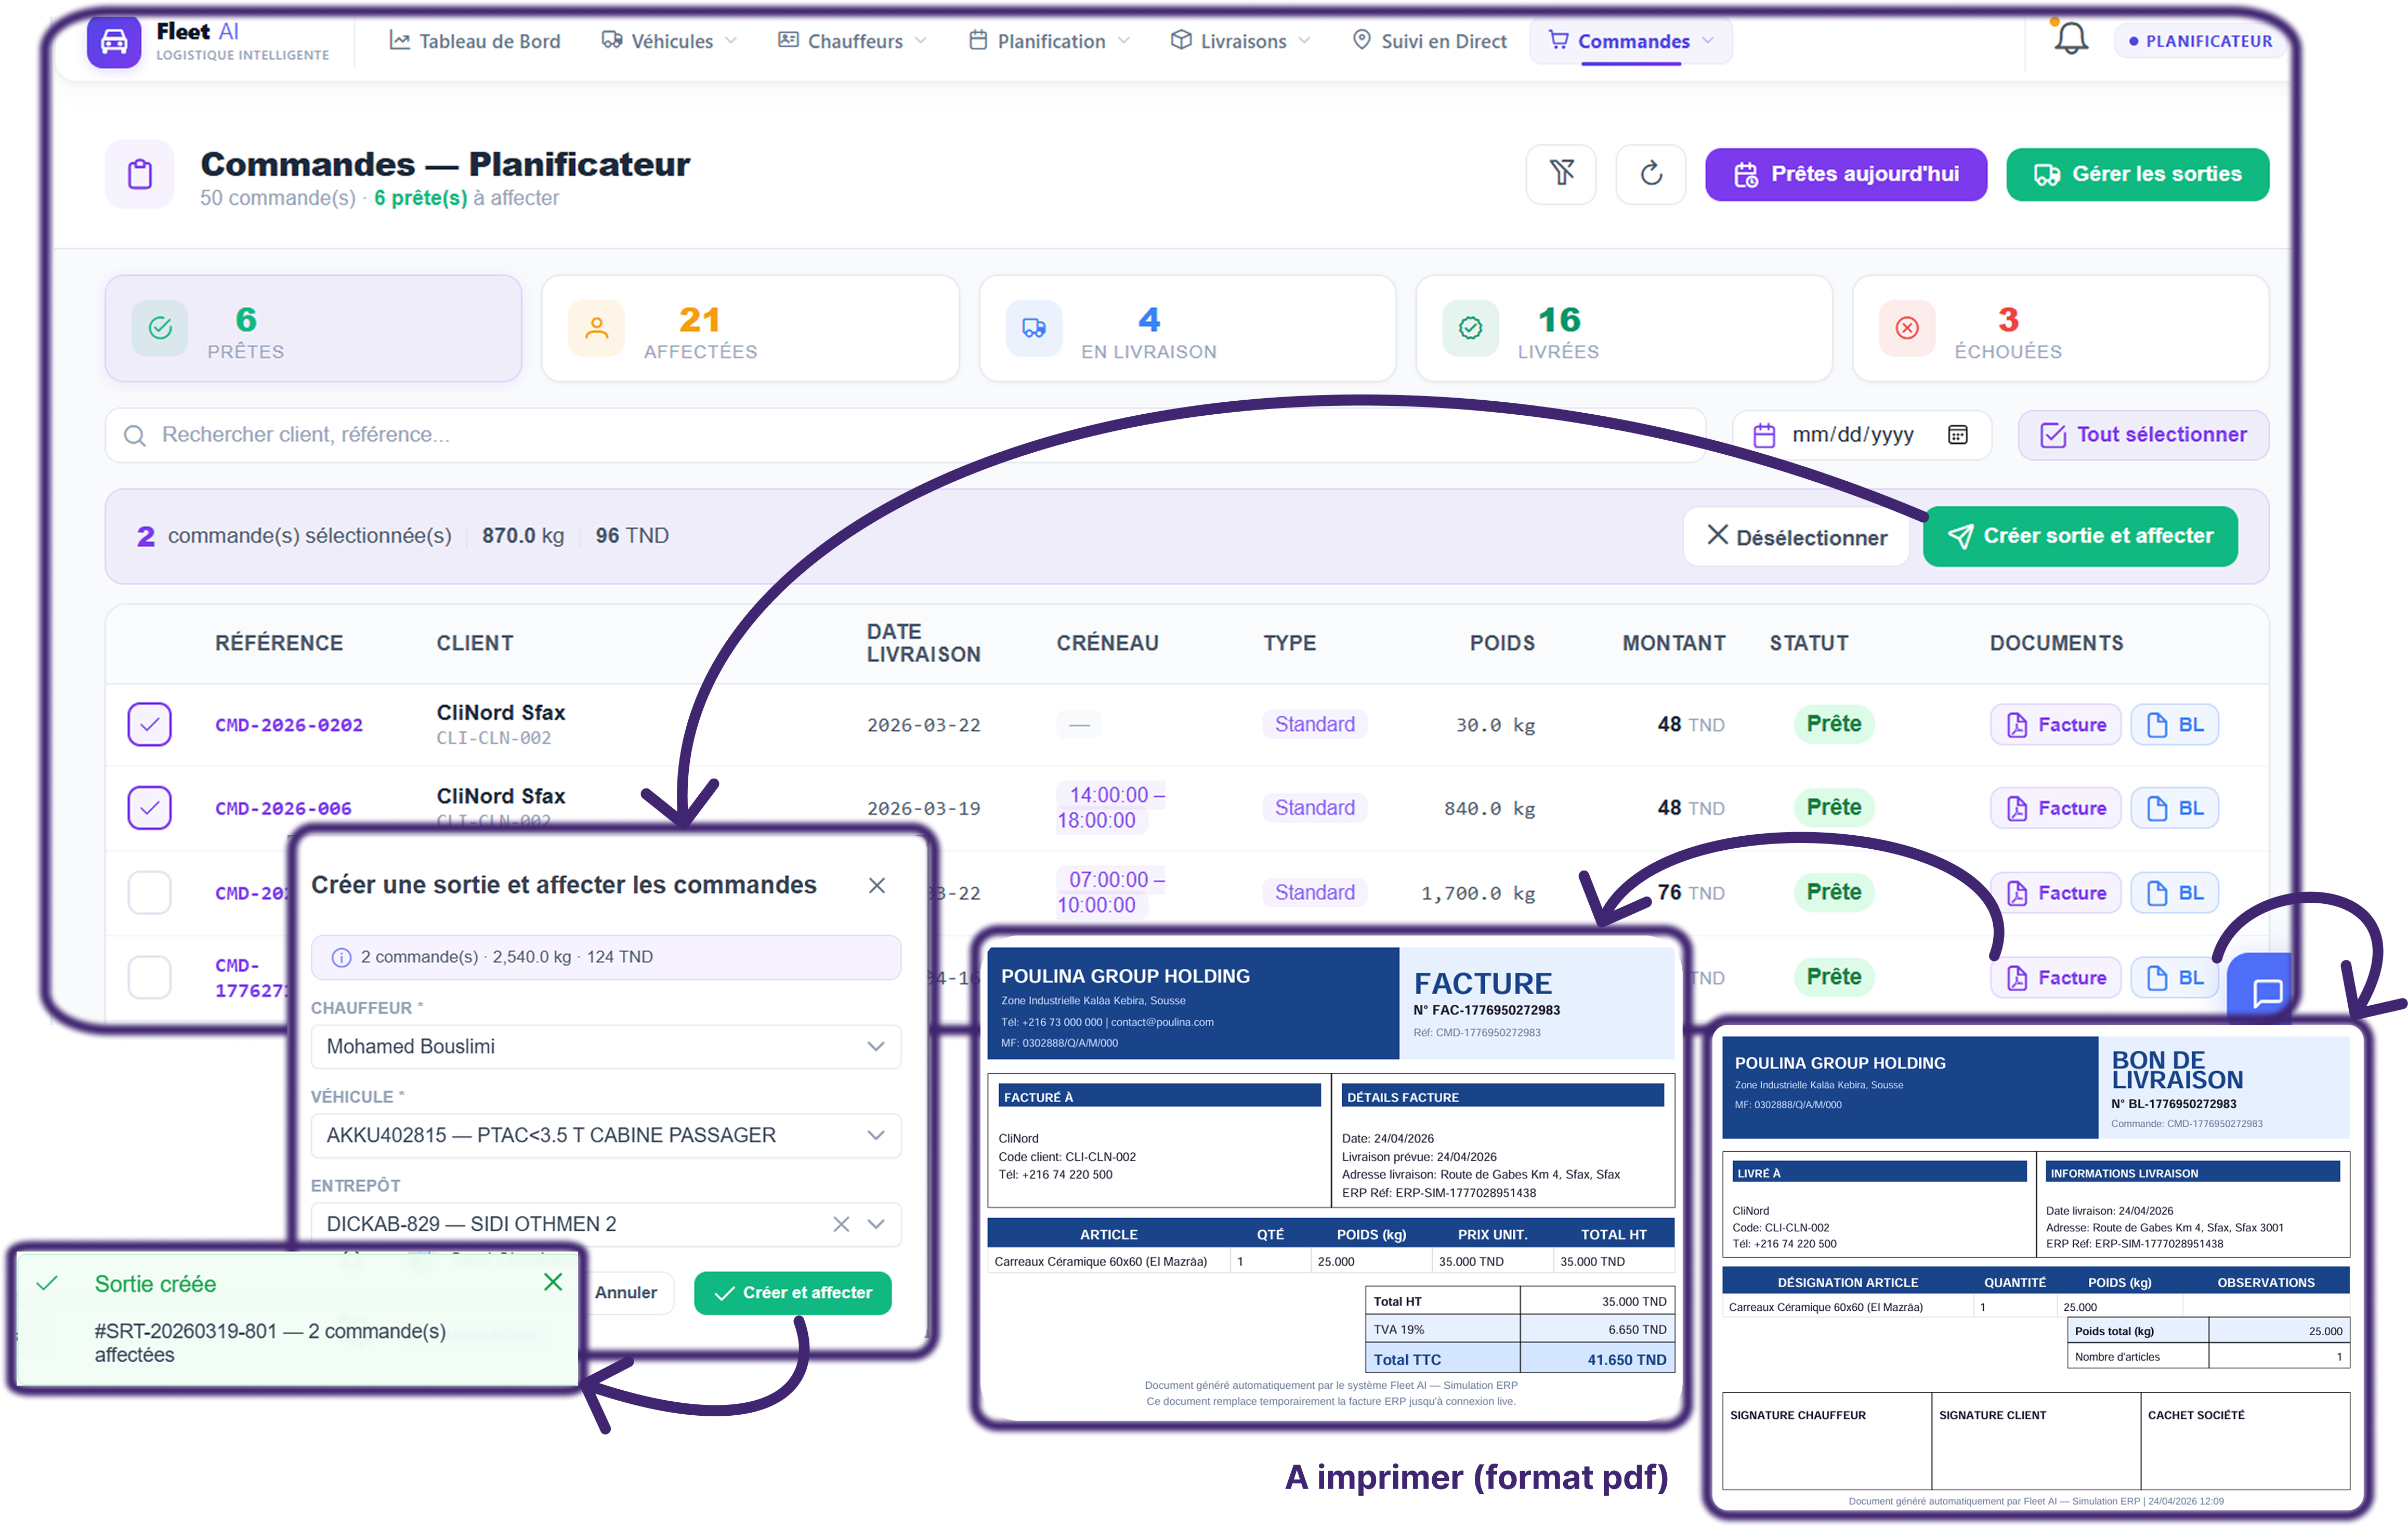
\includegraphics[width=\linewidth, keepaspectratio]{img/capture/web/sp3_planning_composite}%
}{%
  \fbox{\parbox{0.9\linewidth}{\centering\vspace{1.5cm}\textit{[img/sp3\_planning\_composite]}\vspace{1.5cm}}}%
}
\caption{Planification : commandes prêtes, charge chauffeurs et surcharge}
\label{fig:sp3-manual}
\end{figure}

% NOTE : Les suggestions d'itinéraires optimisées (OR-Tools / IA) sont traitées dans le Sprint 5 (chap_08.tex).

% NOTE : Le suivi GPS en temps réel et le tableau de bord KPI journalier sont traités dans le Sprint~4
% (section Suivi GPS et tableau de bord de pilotage), car ils relèvent de la phase d'exécution terrain.

\subsection{Gestion de la disponibilité des chauffeurs}

Le système \texttt{resolveWeeklySchedule()} calcule automatiquement le planning hebdomadaire selon le type de contrat : les Officiels sont automatiquement DISPONIBLE du lundi au vendredi, les Prestataires doivent déclarer leur disponibilité. Les absences (CONGE, MALADIE, FORMATION, MISSION) et les JOUR\_FERIE ont la priorité sur toutes les règles.

\begin{figure}[H]
\centering
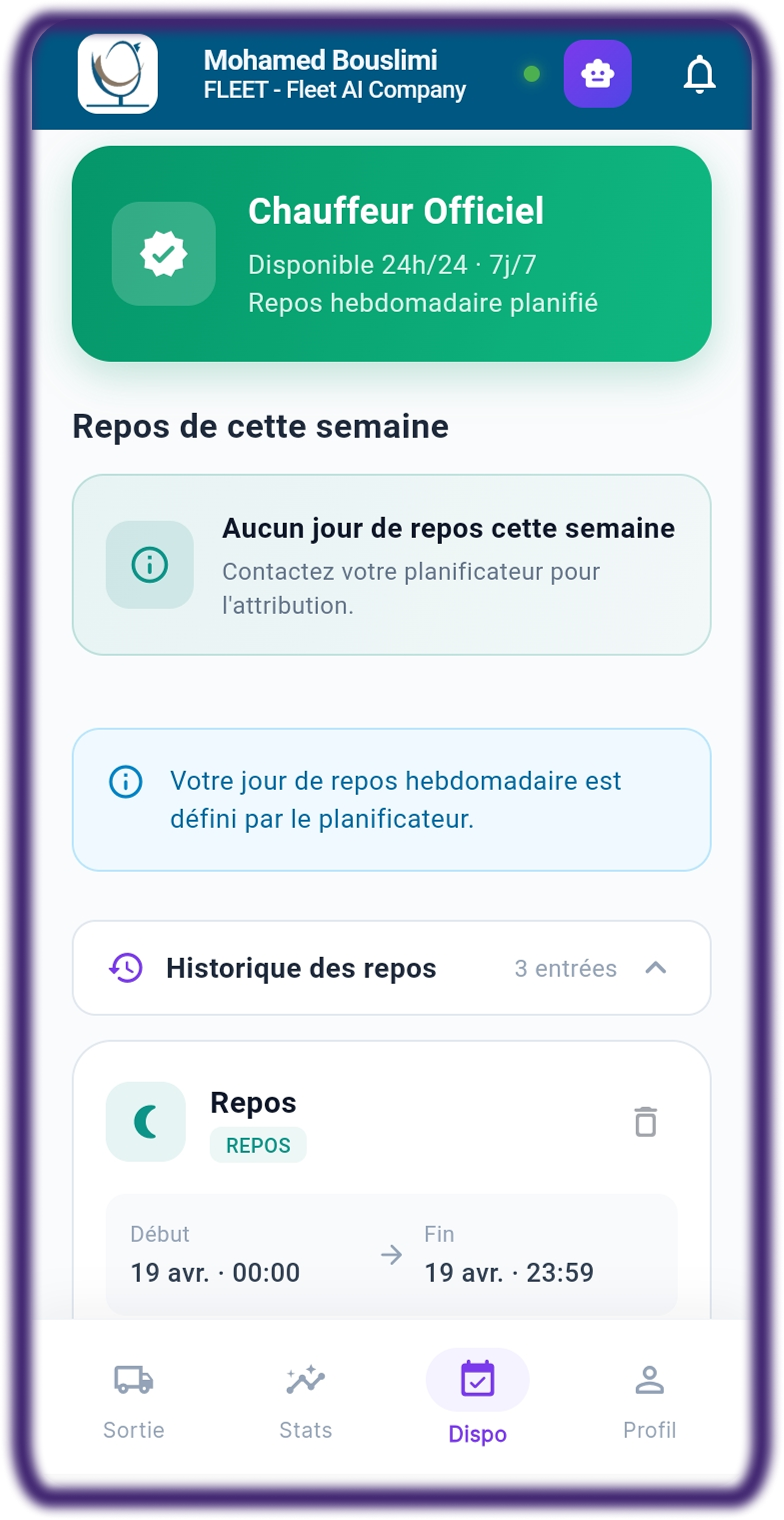
\includegraphics[width=0.48\linewidth, height=0.34\textheight, keepaspectratio]{img/capture/mobile/disponibilite_chauffeur}
\caption{App mobile --- Gestion de la disponibilité}
\label{fig:sp3-availability}
\end{figure}

\subsection{Plans de livraison et bons de chargement}

Le Planificateur regroupe plusieurs commandes par chauffeur dans un plan journalier. Le système calcule les distances estimées (Haversine) et la charge par véhicule. Un bon de chargement listant les articles par commande est générable en un clic.

\begin{figure}[H]
\centering
\IfFileExists{img/capture/web/sp3_plans_composite.png}{%
  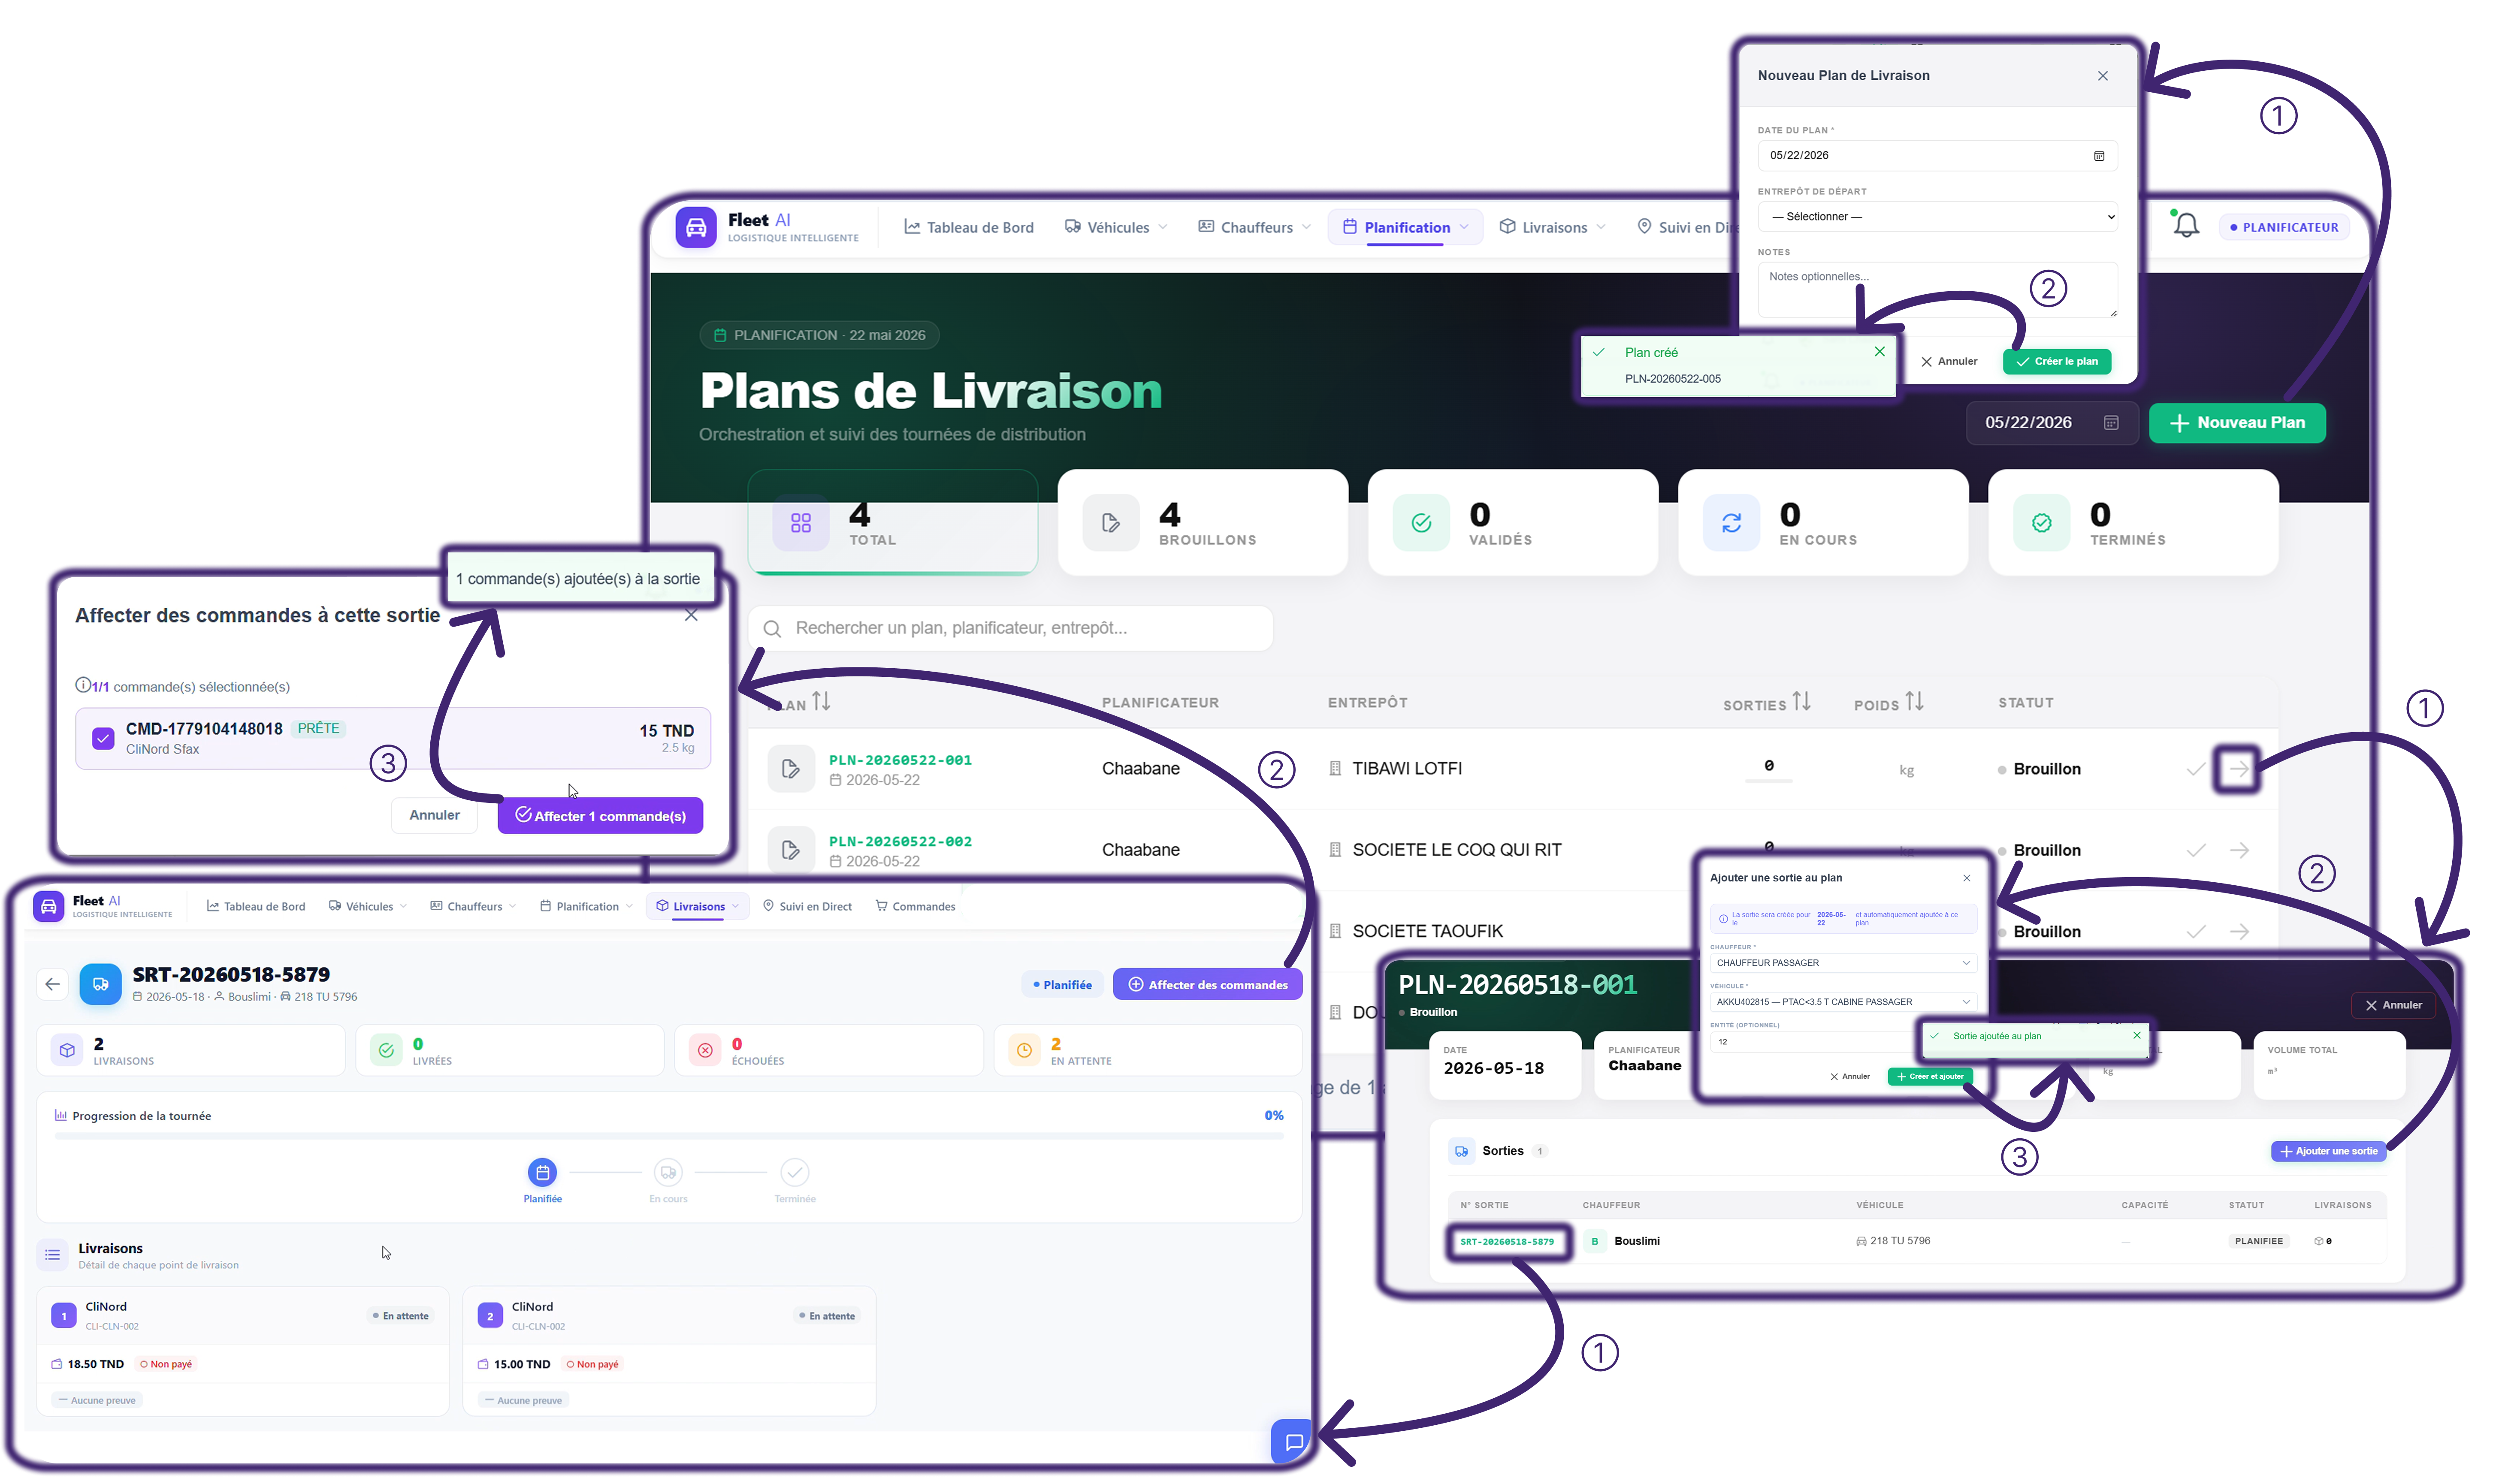
\includegraphics[width=\linewidth, keepaspectratio]{img/capture/web/sp3_plans_composite}%
}{%
  \fbox{\parbox{0.9\linewidth}{\centering\vspace{1.5cm}\textit{[img/sp3\_plans\_composite]}\vspace{1.5cm}}}%
}
\caption{Plans journaliers et bon de chargement PDF}
\label{fig:sp3-plans}
\end{figure}

\subsection{Application mobile Chauffeur --- Itinéraire du jour}

Après validation du plan par le Planificateur, le Chauffeur reçoit son itinéraire sur l'application mobile Fleet~AI (Flutter). Les points de livraison sont affichés numérotés dans l'ordre optimal sur la carte, avec navigation intégrée vers chaque adresse.

\begin{figure}[H]
\centering
\begin{subfigure}[t]{0.38\linewidth}
  \centering
  \IfFileExists{img/capture/mobile/itineraire_flutter.png}{%
    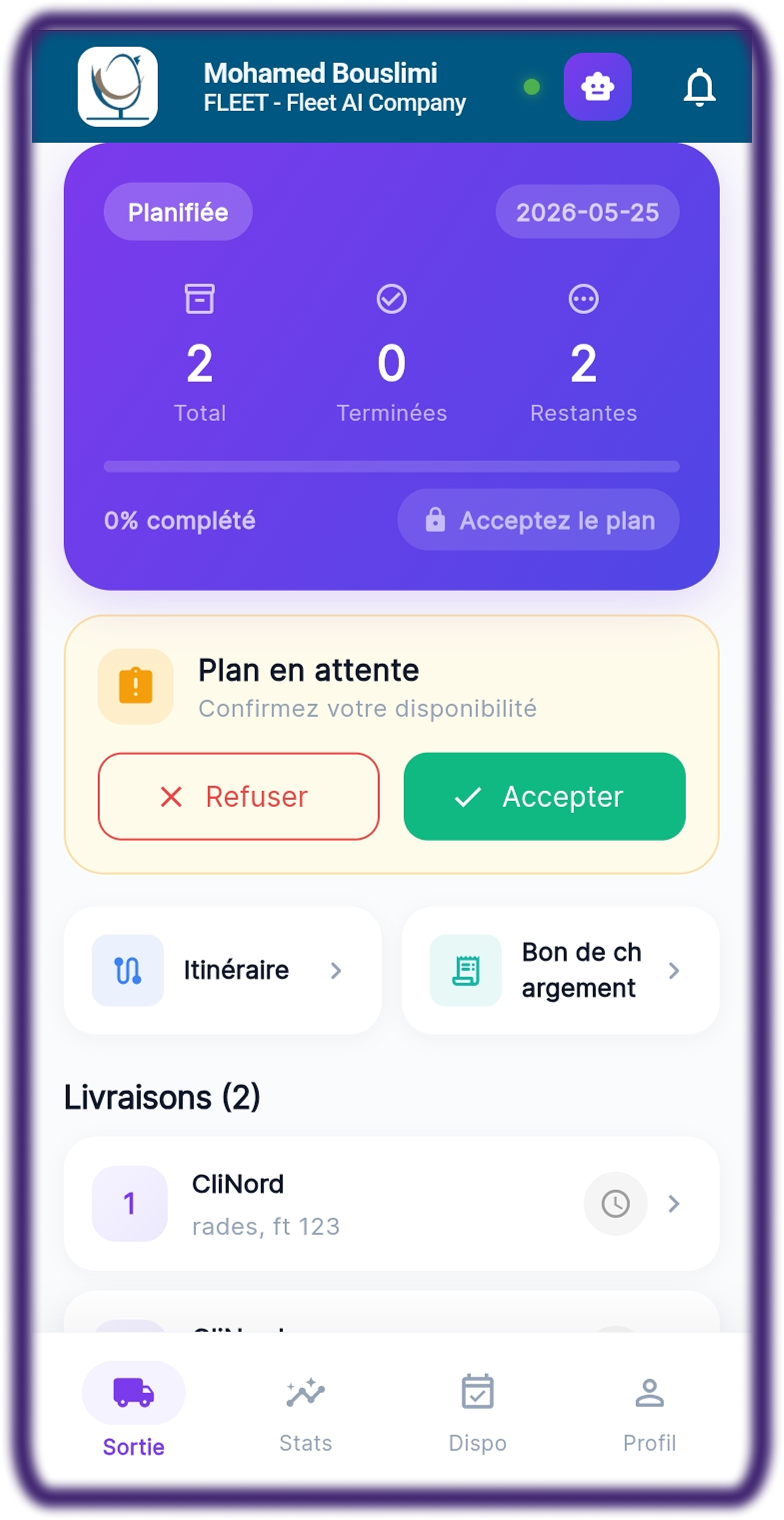
\includegraphics[width=\linewidth, height=0.30\textheight, keepaspectratio]{img/capture/mobile/itineraire_flutter.png}%
  }{%
    \fbox{\parbox{0.9\linewidth}{\centering\vspace{1.5cm}\textit{Manque: itineraire\_flutter.png}\vspace{1.5cm}}}%
  }
  \caption{Itinéraire optimisé sur carte (Flutter)}
\end{subfigure}
\hfill
\begin{subfigure}[t]{0.38\linewidth}
  \centering
  \IfFileExists{img/capture/mobile/liste_livraisons_flutter.png}{%
    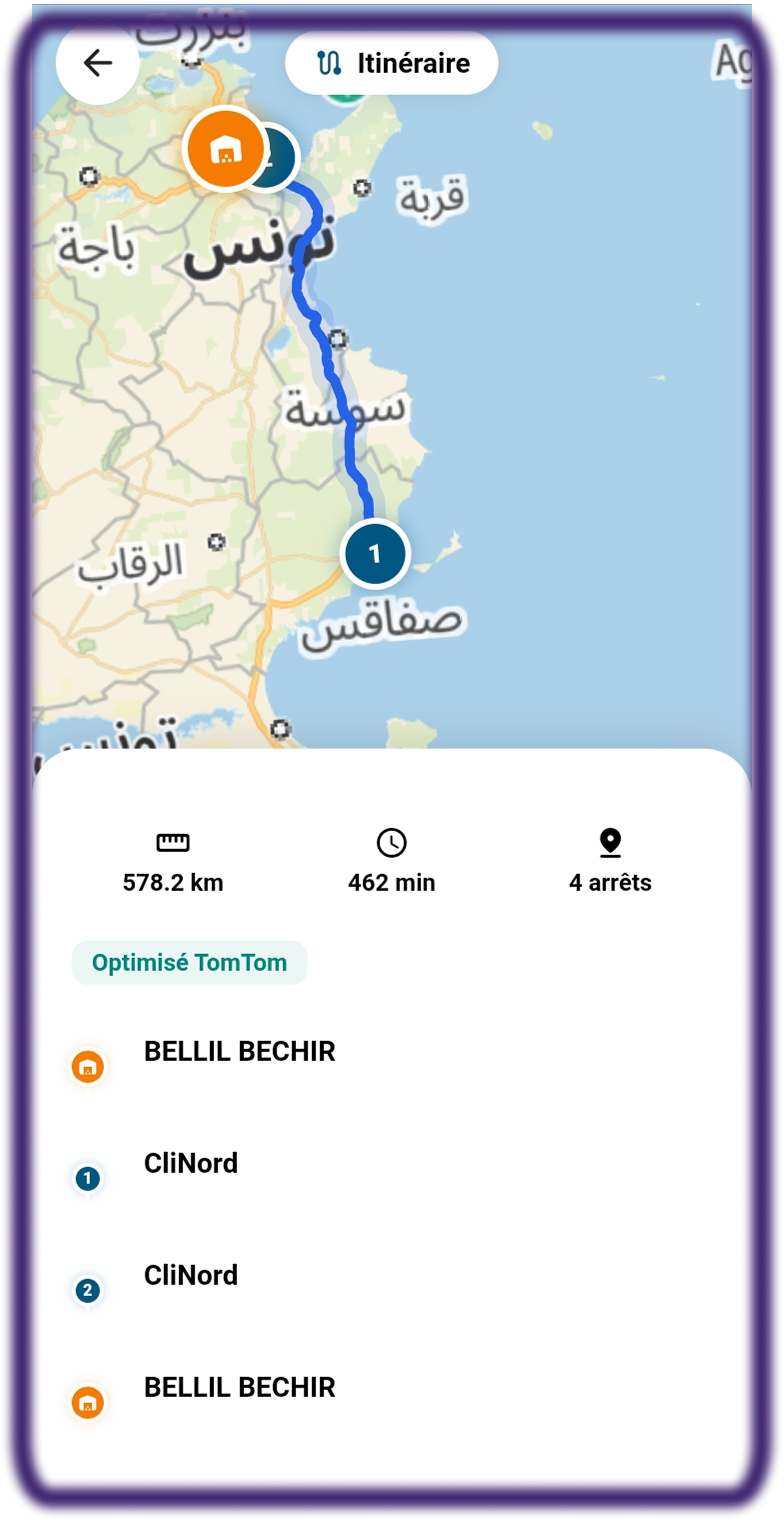
\includegraphics[width=\linewidth, height=0.30\textheight, keepaspectratio]{img/capture/mobile/liste_livraisons_flutter.png}%
  }{%
    \fbox{\parbox{0.9\linewidth}{\centering\vspace{1.5cm}\textit{Manque: liste\_livraisons\_flutter.png}\vspace{1.5cm}}}%
  }
  \caption{Liste des livraisons du jour (Flutter)}
\end{subfigure}
\caption{Application mobile Chauffeur --- Itinéraire et liste des livraisons du jour}
\label{fig:sp3-mobile}
\end{figure}

% =============================================================
\section{Tests}
% =============================================================

Un test d'intégration a été réalisé avec \textbf{Postman} sur l'endpoint \texttt{POST /api/sorties/list}, qui retourne la liste paginée des sorties (missions journalières) selon des critères de filtrage transmis dans le corps de la requête. L'authentification est assurée par l'en-tête \texttt{User-ID} (ici \texttt{sami.chaabane}). Le serveur répond en \textbf{200~OK} avec un payload JSON de 313~Ko en 1,127~seconde, confirmant la conformité du contrat d'API et la performance de la couche de persistance sous charge nominale.

\begin{figure}[H]
\centering
\IfFileExists{img/capture/web/sp3_test_postman_p1.png}{%
  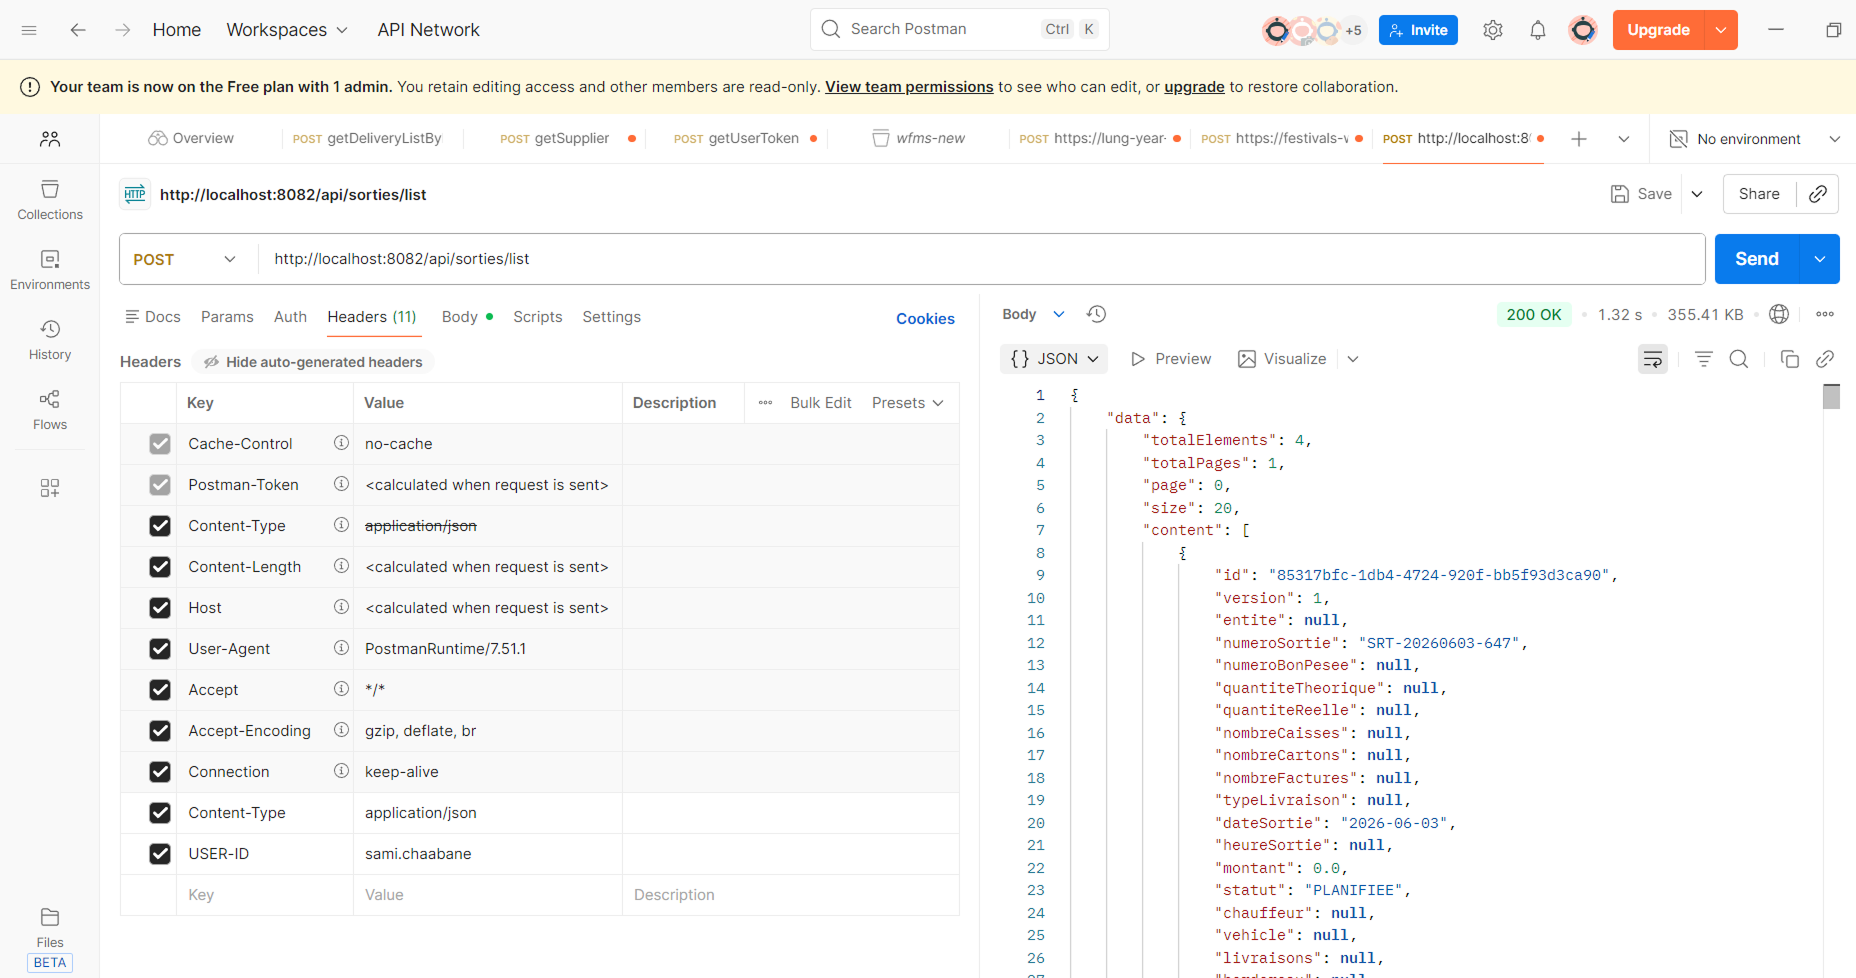
\includegraphics[width=\linewidth, keepaspectratio]{img/capture/web/sp3_test_postman_p1}%
}{%
  \fbox{\parbox{0.9\linewidth}{\centering\vspace{1.5cm}\textit{[img/capture/web/sp3\_test\_postman\_p1.png]}\vspace{1.5cm}}}%
}
\caption{Test Postman --- Endpoint \texttt{POST /api/sorties/list} : requête avec filtres et en-têtes d'authentification (HTTP~200 OK, 313~Ko)}
\label{fig:sp3-test-p1}
\end{figure}

\begin{figure}[H]
\centering
\IfFileExists{img/capture/web/sp3_test_postman_p2.png}{%
  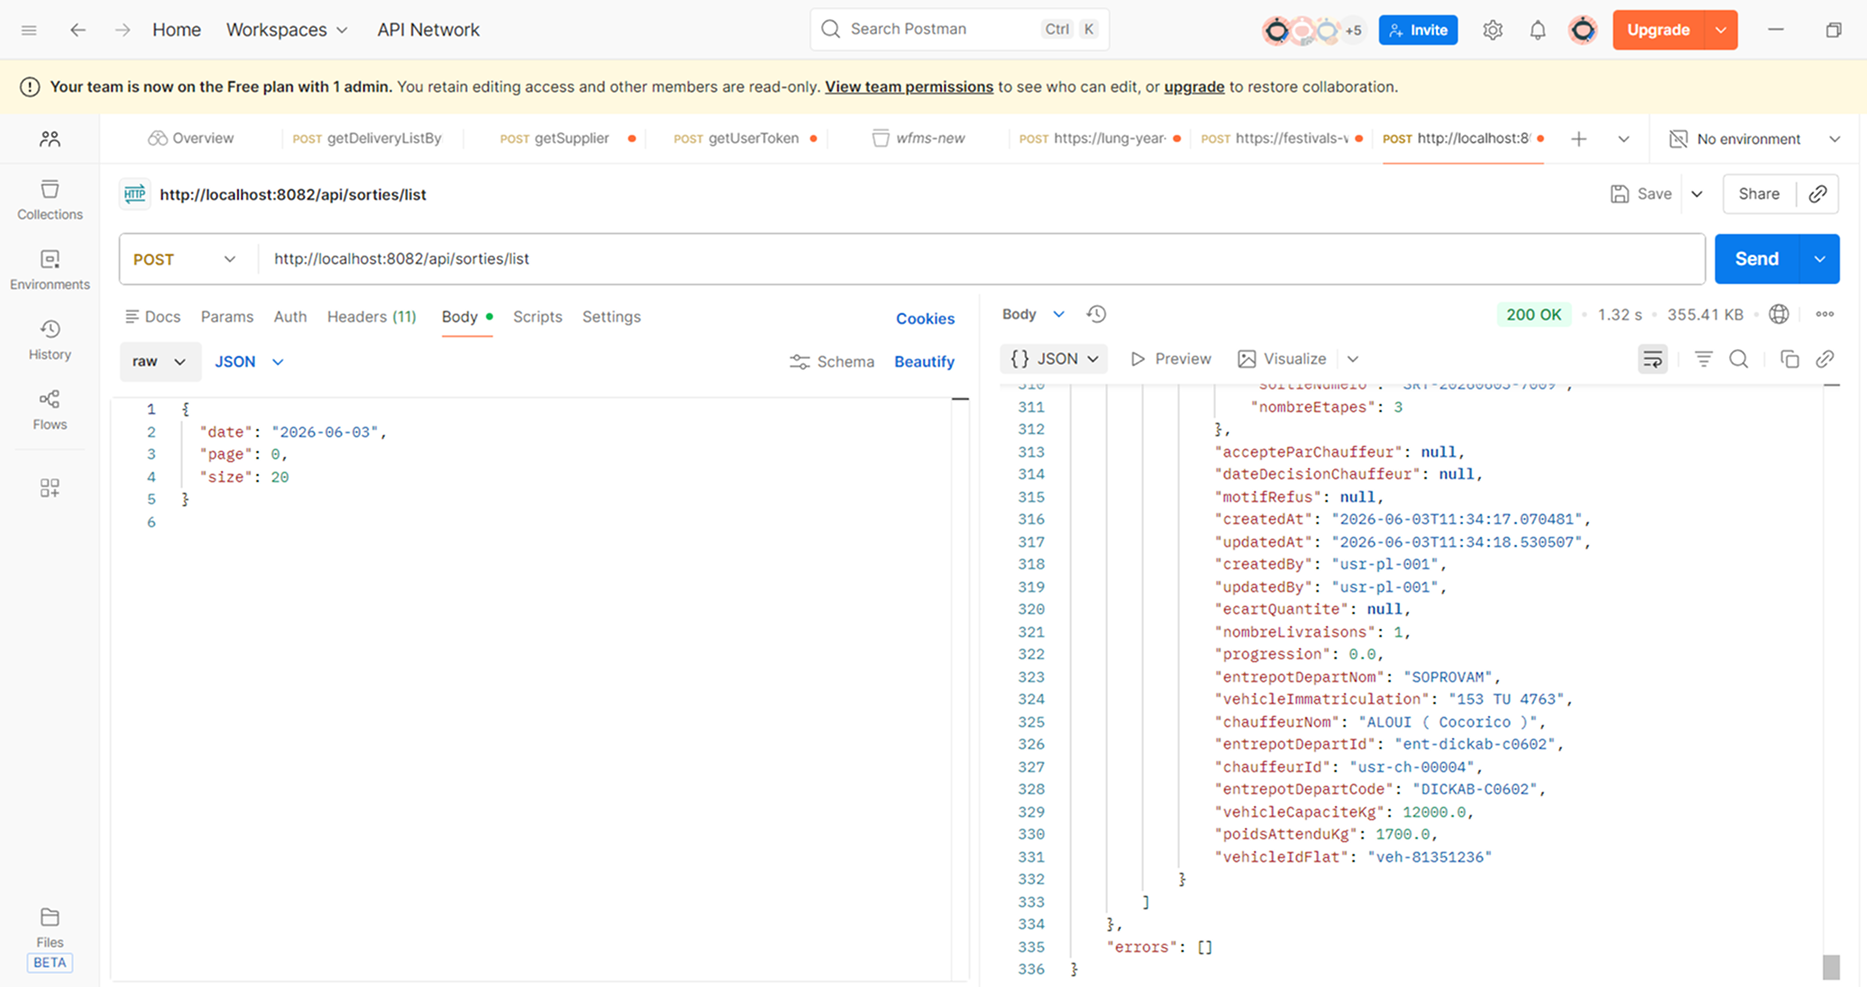
\includegraphics[width=\linewidth, keepaspectratio]{img/capture/web/sp3_test_postman_p2}%
}{%
  \fbox{\parbox{0.9\linewidth}{\centering\vspace{1.5cm}\textit{[img/capture/web/sp3\_test\_postman\_p2.png]}\vspace{1.5cm}}}%
}
\caption{Test Postman --- Réponse paginée de l'endpoint \texttt{POST /api/sorties/list} : liste des sorties avec dates, entités (CLN, PGA), statuts et montants}
\label{fig:sp3-test-p2}
\end{figure}

\section*{Conclusion}
\addcontentsline{toc}{section}{Conclusion}

Le Sprint~3 livre le moteur de planification de Fleet~AI : affectation manuelle avec contrôle de capacité, gestion des disponibilités, plans journaliers et récurrents avec génération de bons de chargement. Le suivi GPS et le tableau de bord de pilotage sont détaillés dans le Sprint~4 ; l'intelligence artificielle dans le Sprint~5.


% ---- Chapitre 7 : Sprint 4 ----
\chapter{Sprint 4 : Exécution des Livraisons, Paiement \& Réclamations}

\section*{Introduction}
\addcontentsline{toc}{section}{Introduction}
Le Sprint~4 couvre l'exécution terrain des livraisons et le pilotage en temps réel. Le Chauffeur dispose sur son application mobile de toutes les fonctionnalités nécessaires pour démarrer une sortie, effectuer une checklist véhicule, valider les livraisons avec preuves numériques (signature, photos géolocalisées, scan d'articles) et traiter les paiements selon trois modes distincts : prépayé, chèque et traite. En cas d'incident, il peut signaler le problème directement depuis l'application. Le Planificateur suit la flotte en temps réel sur une carte GPS avec alertes automatiques de retard. Le REC rapproche les encaissements et traite les réclamations clients, escaladées automatiquement si non résolues dans les délais. Le Manager pilote l'ensemble de l'activité via des tableaux de bord KPI journaliers et des rapports exportables.

\clearpage

\section{Sprint Backlog}

\textbf{Objectif du sprint :} L'objectif est de couvrir l'exécution terrain : validation des livraisons avec preuves numériques, gestion des trois modes de paiement, suivi GPS en temps réel avec alertes de retard, traitement des réclamations avec escalade automatique et mode hors ligne mobile.

\definecolor{headerbg}{HTML}{d5f5e3}
\setlength{\arrayrulewidth}{1pt}

Les story points (SP) reflètent la complexité et l'effort de chaque tâche, estimés selon la suite de Fibonacci.

\begin{longtable}{|>{\raggedright\arraybackslash}p{4.2cm}|>{\raggedright\arraybackslash}p{4.8cm}|>{\raggedright\arraybackslash}p{4.5cm}|c|}
\hline
\rowcolor{headerbg}
\textbf{User Story} & \textbf{Tâche} & \textbf{Critères d'acceptation} & \textbf{\rotatebox{90}{SP}} \\
\hline
\endfirsthead
\hline
\rowcolor{headerbg}
\textbf{User Story} & \textbf{Tâche} & \textbf{Critères d'acceptation} & \textbf{\rotatebox{90}{SP}} \\
\hline
\endhead
\hline
\endfoot

%------ US-039 ------
\multirow{2}{=}{En tant que Chauffeur, je veux démarrer une livraison depuis l'application mobile et voir ses détails afin de préparer ma tournée.}
& Permettre au Chauffeur de consulter les détails d'une livraison (adresse, articles, créneau horaire) avant de la démarrer. & Les détails de la livraison s'affichent sur l'application mobile (adresse, liste d'articles, créneau horaire). & 2 \\
\cline{2-4}
& Mettre à jour automatiquement le statut de la commande au démarrage de la livraison et notifier le Planificateur. & Le statut passe à « En cours de livraison » ; le Planificateur est notifié en temps réel. & 1 \\
\hline

%------ US-040 ------
\multirow{2}{=}{En tant que Chauffeur, je veux confirmer une livraison avec la signature électronique du client depuis l'application mobile.}
& Permettre au Chauffeur de recueillir la signature du client sur écran tactile lors de la remise de commande. & La signature est capturée sur écran tactile, horodatée et transmise au système. & 3 \\
\cline{2-4}
& Faire passer la livraison au statut « Livrée » lors de la confirmation avec signature et notifier les parties concernées. & La livraison passe au statut « Livrée » ; la signature est rattachée à la livraison et consultable. & 2 \\
\hline

%------ US-041 ------
\multirow{2}{=}{En tant que Chauffeur, je veux prendre des photos géolocalisées comme preuve de livraison depuis l'application mobile.}
& Permettre au Chauffeur de prendre des photos géolocalisées lors de chaque livraison. & Les photos sont géolocalisées avec horodatage ; plusieurs photos peuvent être prises par livraison. & 2 \\
\cline{2-4}
& Rattacher les photos prises à la livraison concernée et les rendre consultables par le REC et le Manager. & Les photos sont consultables par le REC et le Manager dans l'historique de la livraison. & 1 \\
\hline

%------ US-042 ------
\multirow{2}{=}{En tant que Chauffeur, je veux valider les articles livrés depuis l'application mobile afin de confirmer la conformité de la commande.}
& Permettre au Chauffeur de valider les articles remis au client et détecter tout écart avec la commande prévue. & La validation des articles est réalisée ; tout écart entre les articles prévus et livrés génère une alerte. & 2 \\
\cline{2-4}
& Notifier le REC de tout écart constaté entre les articles prévus et effectivement livrés. & Un écart entre prévu et livré génère une alerte visible par le REC. & 1 \\
\hline

%------ US-043 ------
\multirow{2}{=}{En tant que Chauffeur, je veux signaler un problème de livraison depuis l'application mobile.}
& Permettre au Chauffeur de sélectionner le type de problème rencontré parmi une liste de motifs prédéfinis. & Le type de problème est sélectionné ; commentaire optionnel ; le statut de la livraison passe à « Échouée ». & 2 \\
\cline{2-4}
& Notifier automatiquement le Planificateur et le REC après le signalement d'un problème par le Chauffeur. & Le Planificateur et le REC reçoivent une notification immédiate avec les détails du problème. & 1 \\
\hline

%------ US-044 ------
\multirow{2}{=}{En tant que Planificateur, je veux suivre en temps réel la position des chauffeurs dans mon tableau de bord afin de superviser les tournées.}
& Afficher au Planificateur la position en temps réel de tous les chauffeurs actifs sur une carte. & La carte affiche tous les chauffeurs actifs ; les positions sont mises à jour régulièrement. & 3 \\
\cline{2-4}
& Afficher les alertes de retard directement sur la carte de suivi avec possibilité de filtrer par zone. & Les alertes de retard s'affichent automatiquement ; le filtrage par zone est disponible. & 2 \\
\hline

%------ US-045 ------
\multirow{2}{=}{En tant que Planificateur, je veux que le statut de la commande se mette à jour automatiquement à chaque action du Chauffeur afin de suivre l'avancement en temps réel.}
& Déclencher automatiquement les transitions de statut de la commande à partir des actions du Chauffeur sur l'application mobile. & Chaque action du Chauffeur déclenche la mise à jour du statut ; synchronisation en temps réel. & 2 \\
\cline{2-4}
& Notifier les parties prenantes concernées (REC, Client) à chaque changement de statut de la commande. & Les notifications sont envoyées aux bonnes parties prenantes à chaque transition de statut. & 1 \\
\hline

%------ US-046 ------
\multirow{2}{=}{En tant que REC, je veux générer un bordereau de livraison pour chaque tournée depuis mon application web.}
& Générer un document récapitulatif de tournée (bordereau) listant les livraisons, les articles et les clients concernés. & Le bordereau contient la liste des livraisons, les articles et les clients ; téléchargeable. & 2 \\
\cline{2-4}
& Permettre au REC de télécharger le bordereau depuis l'interface de gestion des tournées en un clic. & Le bordereau est généré et téléchargeable depuis l'interface en un clic. & 1 \\
\hline

%------ US-047 ------
\multirow{2}{=}{En tant que Chauffeur, je veux remplir un checklist de départ du véhicule sur l'application mobile avant le début de la journée.}
& Permettre au Chauffeur de remplir une liste de contrôles de départ avec prise de photos pour les anomalies constatées. & Le checklist est interactif ; les anomalies sont documentées avec photos. & 2 \\
\cline{2-4}
& Bloquer le démarrage de la tournée si les points critiques du checklist ne sont pas validés par le Chauffeur. & Le démarrage est bloqué si des points critiques ne sont pas validés ; une alerte est affichée. & 1 \\
\hline

%------ US-048 ------
\multirow{2}{=}{En tant que Client, je veux suivre ma livraison en temps réel sur une carte dans l'application mobile.}
& Afficher au Client la position du chauffeur sur une carte avec estimation de l'heure d'arrivée. & Le Client voit la position du chauffeur sur la carte ; l'estimation d'arrivée est mise à jour régulièrement. & 3 \\
\cline{2-4}
& Envoyer une notification au Client lorsque le chauffeur est à moins de 10 minutes de son adresse. & La notification est envoyée lorsque le chauffeur est à moins de 10 minutes de l'adresse. & 2 \\
\hline

%------ US-049 ------
\multirow{2}{=}{En tant que Planificateur, je veux que le système détecte automatiquement les retards et l'alerte afin de prendre des mesures correctives.}
& Détecter automatiquement un retard lorsqu'une livraison dépasse de plus de 15 minutes l'estimation initiale. & Une alerte est générée si le retard dépasse 15 minutes ; le statut de retard est affiché. & 2 \\
\cline{2-4}
& Notifier le Planificateur et le REC en cas de retard détecté avec les détails de la livraison concernée. & Le Planificateur et le REC reçoivent une alerte dans les 2 minutes suivant la détection. & 1 \\
\hline

%------ Mode 1 - Prépayé ------
\multirow{2}{=}{En tant que Planificateur, je veux voir le statut de paiement d'une commande afin d'autoriser ou bloquer la livraison.}
& Importer le statut de paiement depuis le système de gestion des commandes et l'afficher sur la fiche commande. & Le statut de paiement est importé avec la commande ; si prépayé, la livraison est autorisée automatiquement. & 2 \\
\cline{2-4}
& Afficher un indicateur « Prépayé » sur la commande visible par le Planificateur et le Chauffeur. & L'indicateur de paiement est visible sur l'interface web (Planificateur) et l'application mobile (Chauffeur). & 1 \\
\hline

%------ Mode 2 - Chèque ------
\multirow{2}{=}{En tant que Chauffeur, je veux photographier le chèque du client et l'envoyer au REC pour validation avant d'autoriser la livraison.}
& Permettre au Chauffeur de photographier le chèque et de l'envoyer en temps réel au REC pour traitement. & La photo est transmise et reçue par le REC en temps réel ; les informations du chèque sont extraites automatiquement. & 3 \\
\cline{2-4}
& Permettre au REC de valider le chèque et d'envoyer une autorisation de livraison au Chauffeur. & La validation par le REC déclenche une autorisation envoyée au Chauffeur ; en cas d'échec, le motif est communiqué. & 5 \\
\hline

%------ Mode 3 - Traite ------
\multirow{2}{=}{En tant que Chauffeur, je veux photographier une traite et l'envoyer au REC pour décision d'acceptation ou refus.}
& Permettre au Chauffeur de photographier la traite et de l'envoyer au REC pour décision. & La photo est transmise et reçue par le REC ; l'acceptation autorise la livraison ; le refus exige un motif. & 3 \\
\cline{2-4}
& Notifier le Chauffeur de la décision du REC (acceptation = livraison autorisée ; refus = retour marchandise). & Acceptation : livraison autorisée. Refus : motif enregistré et Chauffeur et Client notifiés. & 2 \\
\hline

%------ US-050 ------
\multirow{2}{=}{En tant que Manager, je veux consulter les indicateurs de livraison du jour dans mon tableau de bord.}
& Calculer et exposer au Manager les indicateurs de livraison du jour (livrées, en cours, en retard, échouées). & Le tableau de bord affiche les compteurs par statut mis à jour en temps réel. & 2 \\
\cline{2-4}
& Afficher au Manager les indicateurs de livraison du jour avec graphique d'évolution. & Les indicateurs s'actualisent automatiquement ; le taux de réussite et le graphique d'évolution sont affichés. & 1 \\
\hline

%------ US-063-067 ------
\multirow{2}{=}{En tant que Chauffeur, je veux consulter le récapitulatif de mes encaissements du jour depuis l'application mobile.}
& Calculer et exposer au Chauffeur le récapitulatif de ses encaissements du jour par mode de paiement et par montant. & Le récapitulatif affiche le total par mode (espèces, chèques, traites) et le nombre de transactions. & 2 \\
\cline{2-4}
& Afficher au Chauffeur l'écran d'encaissements avec liste détaillée et totaux par mode de paiement. & L'écran est accessible depuis l'application mobile ; les totaux sont corrects et mis à jour. & 1 \\
\hline

%------ US-068 ------
\multirow{2}{=}{En tant que REC, je veux rapprocher les encaissements avec les commandes livrées dans mon application web.}
& Permettre au REC de rapprocher les encaissements reçus avec les commandes livrées et de détecter les écarts. & L'association encaissement/commande fonctionne ; les écarts sont signalés et mis en évidence. & 3 \\
\cline{2-4}
& Afficher au REC la liste des encaissements avec indicateurs d'écarts et statut de rapprochement. & Le statut « Rapproché » est visible ; les écarts sont mis en évidence pour action corrective. & 2 \\
\hline

%------ US-105/107 ------
\multirow{2}{=}{En tant que Manager, je veux un tableau de bord stratégique avec export des rapports et visualisation des tendances.}
& Calculer les indicateurs stratégiques (taux de livraison, coût par kilomètre, satisfaction client, utilisation de la flotte) et les exposer au Manager. & Les indicateurs stratégiques sont disponibles avec comparaison par période. & 3 \\
\cline{2-4}
& Permettre au Manager d'exporter les rapports et de visualiser les tendances sur 30, 60 et 90 jours. & Les rapports sont exportables ; les graphiques de tendances sur 30/60/90 jours sont disponibles. & 2 \\
\hline


%------ US-105 ------
\multirow{2}{=}{En tant que Client, je veux soumettre une réclamation depuis l'application mobile afin d'obtenir un suivi.}
& Permettre au Client de soumettre une réclamation en précisant la catégorie, la description et des photos jointes. & La réclamation est créée avec catégorie, description et pièces jointes ; un numéro de suivi est généré. & 3 \\
\cline{2-4}
& Affecter automatiquement la réclamation au Responsable en charge du client concerné. & La réclamation est assignée au Responsable du client ; un numéro de ticket est communiqué au Client. & 2 \\
\hline

%------ US-106 ------
\multirow{2}{=}{En tant que Responsable des Engagements Clients, je veux voir la liste des réclamations et les traiter dans le respect du délai de service.}
& Mettre à disposition du REC la liste des réclamations avec filtres par statut, date et délai de service restant. & Les réclamations sont filtrables ; le délai de service restant (en jours) est affiché pour chaque réclamation. & 3 \\
\cline{2-4}
& Permettre au REC de prendre en charge, résoudre ou clôturer une réclamation avec notification au Client à chaque changement. & Le REC peut changer le statut ; le Client est notifié à chaque changement de statut. & 2 \\
\hline

%------ US-107 ------
\multirow{2}{=}{En tant que Client, je veux suivre le statut de ma réclamation depuis l'application mobile afin de rester informé de son traitement.}
& Permettre au Client de consulter l'état de sa réclamation avec l'historique des transitions de statut. & Le Client voit le statut en temps réel avec l'historique des transitions. & 2 \\
\cline{2-4}
& Notifier le Client à chaque changement de statut de sa réclamation. & Le Client est notifié en temps réel à chaque changement de statut. & 1 \\
\hline

%------ US-108/110 ------
\multirow{2}{=}{En tant que Manager, je veux des statistiques sur les réclamations et l'identification des causes récurrentes dans mon tableau de bord.}
& Calculer les indicateurs de réclamations (volume, délai moyen de traitement, taux de récurrence, causes principales) et les exposer au Manager. & Les statistiques incluent : nombre par catégorie, délai moyen, taux de récurrence. & 3 \\
\cline{2-4}
& Afficher les causes les plus fréquentes de réclamations dans une vue comparative dans le tableau de bord Manager. & Les principales causes de réclamations s'affichent par ordre de fréquence décroissante. & 2 \\
\hline

%------ US-109 ------
\multirow{2}{=}{En tant que Responsable des Engagements Clients, je veux que les réclamations non traitées soient escaladées automatiquement après 48 heures afin de respecter les délais de réponse.}
& Déclencher automatiquement l'escalade d'une réclamation non traitée après 48 heures avec notification au Manager. & L'escalade est déclenchée après 48 heures ; le Manager est notifié avec les détails de la réclamation. & 2 \\
\cline{2-4}
& Mettre en évidence les réclamations escaladées dans la liste du REC avec un indicateur d'urgence visible. & Les réclamations escaladées affichent un indicateur d'urgence dans la liste. & 1 \\
\hline

%------ US-119/120 ------
\multirow{2}{=}{En tant que Manager, je veux personnaliser mon tableau de bord avec des widgets configurables et exporter les rapports.}
& Permettre au Manager de réorganiser les widgets de son tableau de bord et de sauvegarder sa configuration. & Les widgets sont déplaçables ; la configuration est sauvegardée par profil utilisateur. & 3 \\
\cline{2-4}
& Permettre au Manager d'exporter les rapports du tableau de bord dans des formats standards. & Les rapports sont exportables depuis tous les tableaux de bord ; la mise en page est professionnelle. & 2 \\
\hline

%------ US-140/141/142 ------
\multirow{2}{=}{En tant que Chauffeur, je veux utiliser l'application mobile en mode hors ligne et que mes actions se synchronisent automatiquement au retour du réseau.}
& Permettre au Chauffeur d'utiliser les fonctionnalités essentielles de l'application sans connexion réseau, avec mise en file d'attente des actions. & Les données essentielles sont disponibles hors ligne ; les actions sont mises en file d'attente et exécutées au retour du réseau. & 5 \\
\cline{2-4}
& Synchroniser automatiquement les données au retour du réseau avec gestion des conflits éventuels et indicateur de statut de connexion. & La synchronisation démarre automatiquement ; les conflits critiques sont signalés ; un indicateur de connexion est visible. & 3 \\
\hline

%------ US-121/122/123 ------
\multirow{2}{=}{En tant que Manager, je veux voir les tendances sur 30, 60 et 90 jours et un tableau de bord de performance des chauffeurs avec rapports automatisés.}
& Calculer les indicateurs historiques sur 30, 60 et 90 jours avec détection des anomalies et les présenter au Manager. & Les graphiques affichent les tendances ; les anomalies sont détectées et mises en évidence. & 3 \\
\cline{2-4}
& Envoyer automatiquement des rapports récapitulatifs hebdomadaires aux destinataires configurés. & Les rapports hebdomadaires sont envoyés automatiquement aux destinataires configurés. & 2 \\
\hline

\caption{Sprint Backlog du Sprint 4 --- Exécution des Livraisons, Paiement \& Réclamations}
\end{longtable}
\setlength{\arrayrulewidth}{0.4pt}


% =============================================================
\section{Conception}
% =============================================================

\subsection{Diagramme de cas d'utilisation}

\begin{figure}[H]
\centering
\IfFileExists{img/diagrammes/sprint_4_usecase_p1.png}{%
  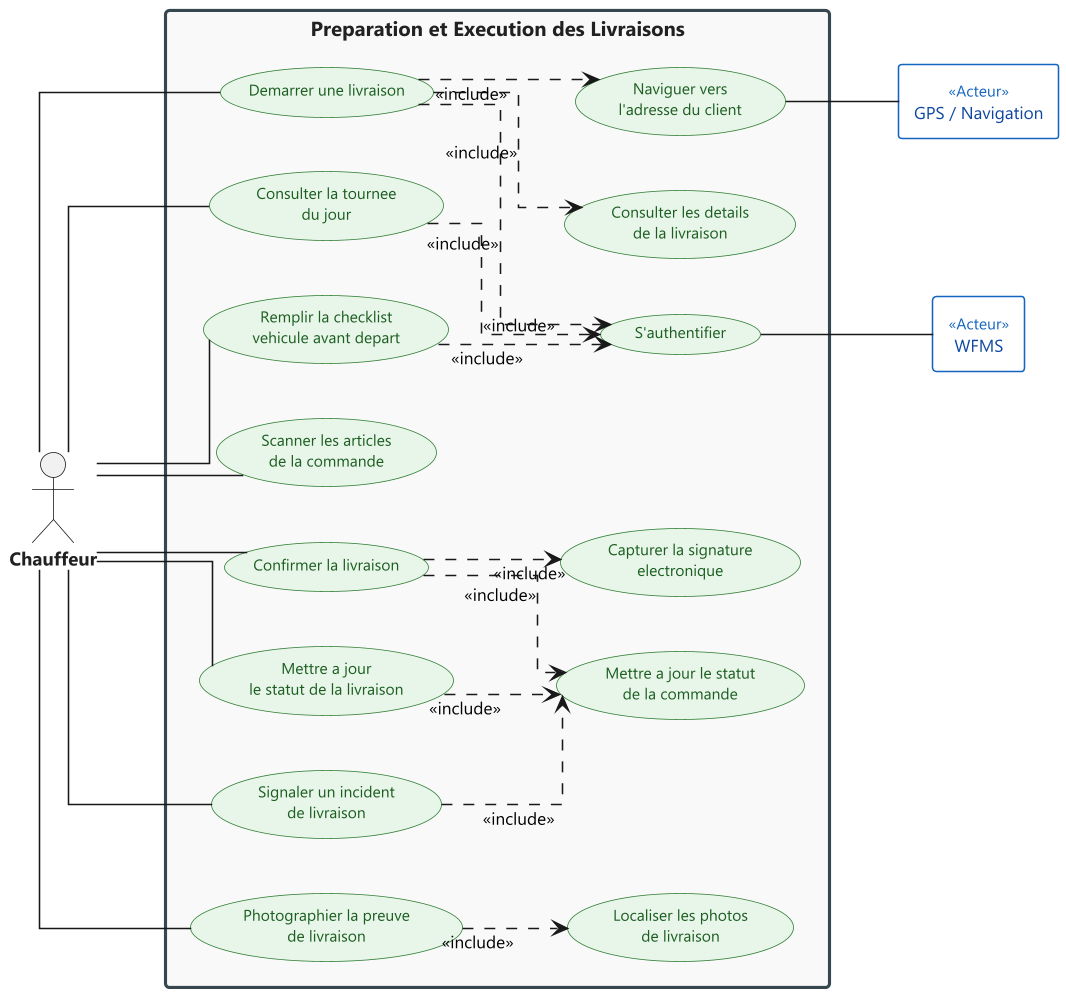
\includegraphics[width=0.9\textwidth, height=0.85\textheight, keepaspectratio]{img/diagrammes/sprint_4_usecase_p1}%
}{%
  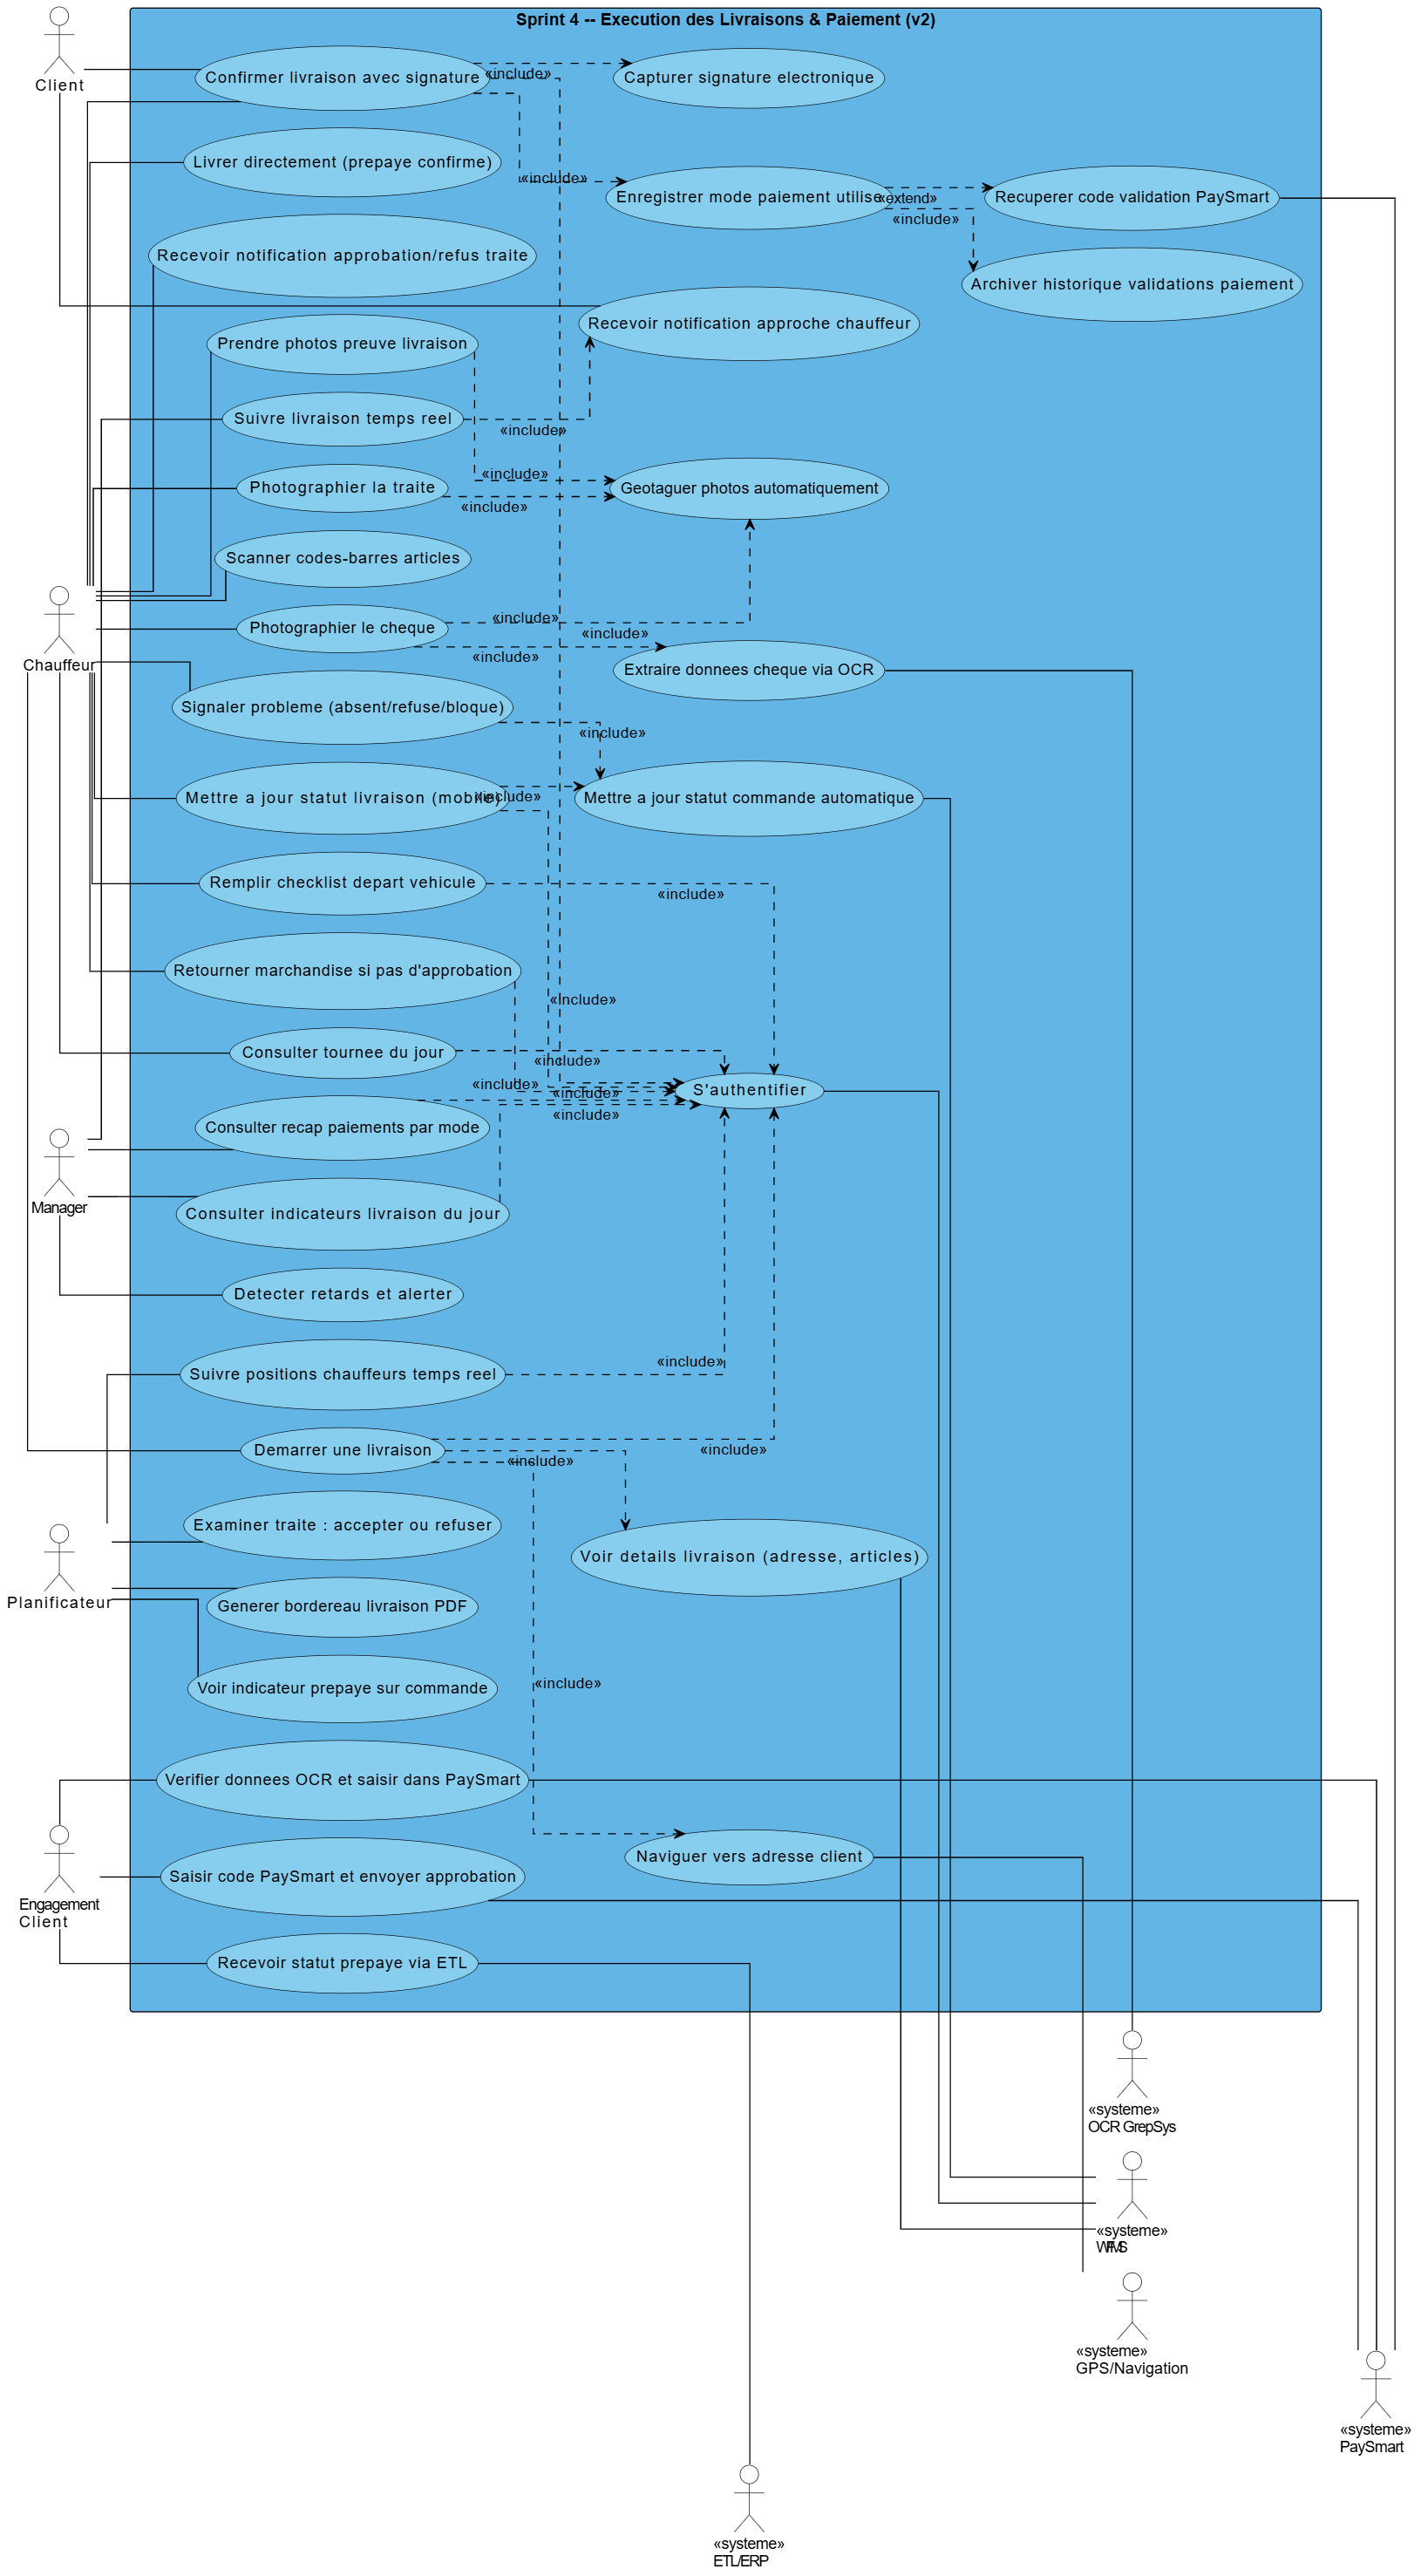
\includegraphics[width=0.9\textwidth, height=0.85\textheight, keepaspectratio]{img/diagrammes/sprint_4_usecase}%
}
\caption{Diagramme de cas d'utilisation du Sprint~4 --- Partie~1}
\label{fig:cas-utilisation-sp4-p1}
\end{figure}

\begin{figure}[H]
\centering
\IfFileExists{img/diagrammes/sprint_4_usecase_p2.png}{%
  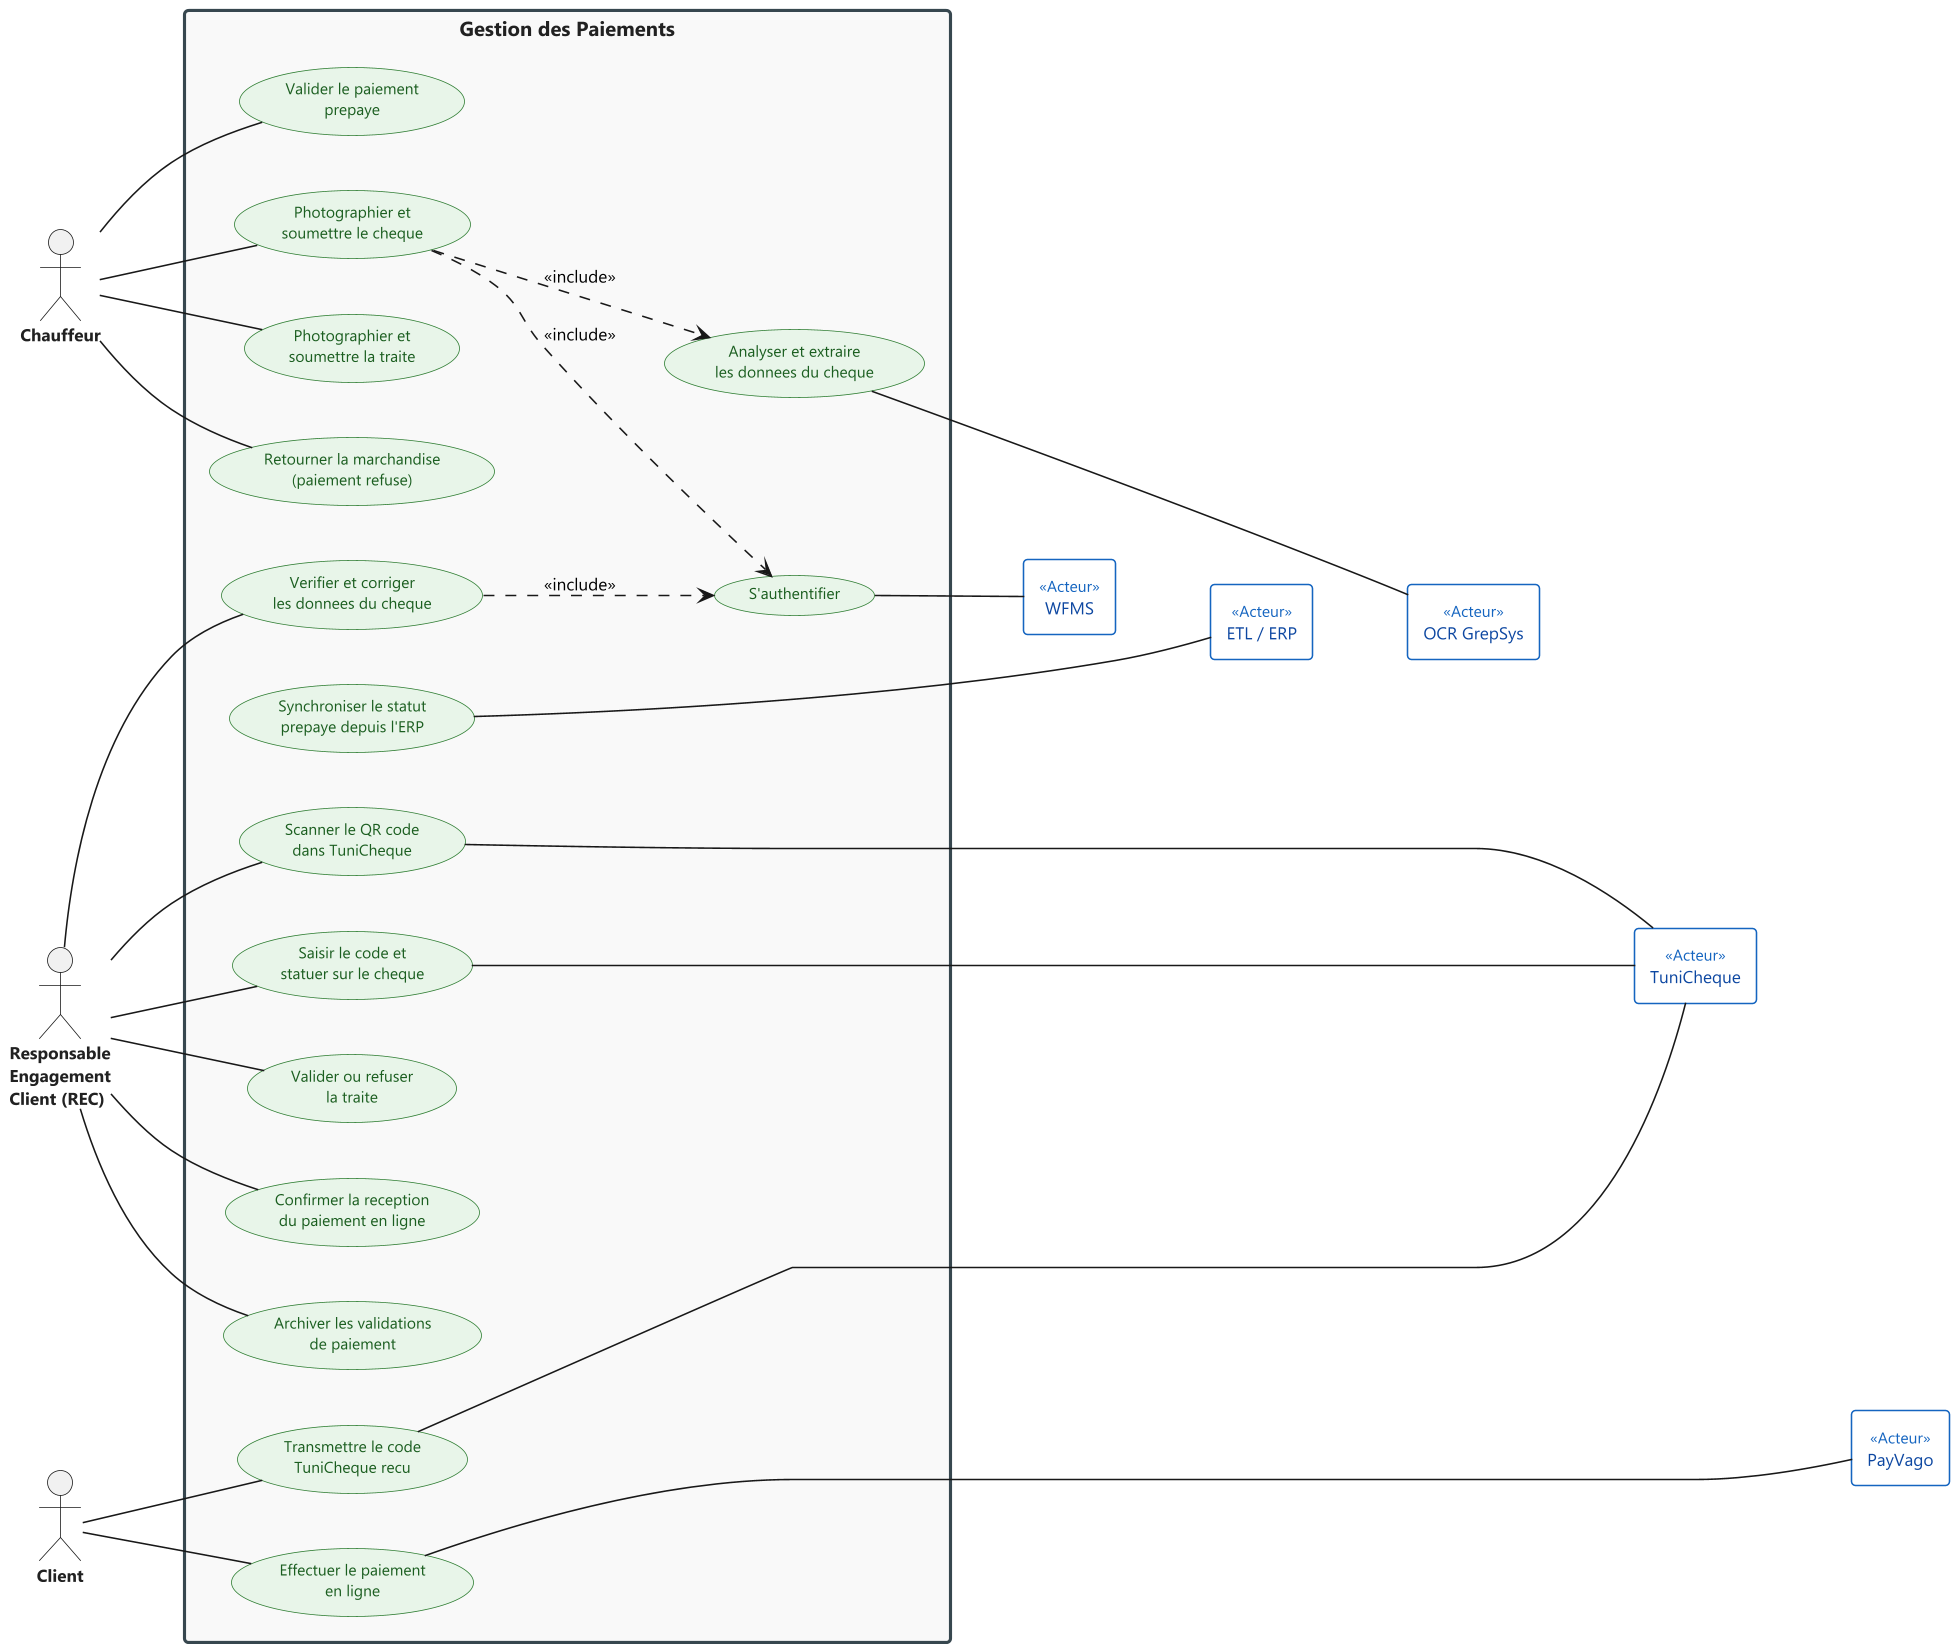
\includegraphics[width=0.9\textwidth, height=0.85\textheight, keepaspectratio]{img/diagrammes/sprint_4_usecase_p2}%
}{%
  \fbox{\parbox{0.9\linewidth}{\centering\vspace{4cm}\textit{[img/diagrammes/sprint\_4\_usecase\_p2.png]}\vspace{4cm}}}%
}
\caption{Diagramme de cas d'utilisation du Sprint~4 --- Partie~2}
\label{fig:cas-utilisation-sp4-p2}
\end{figure}

\begin{figure}[H]
\centering
\IfFileExists{img/diagrammes/sprint_4_usecase_p3.png}{%
  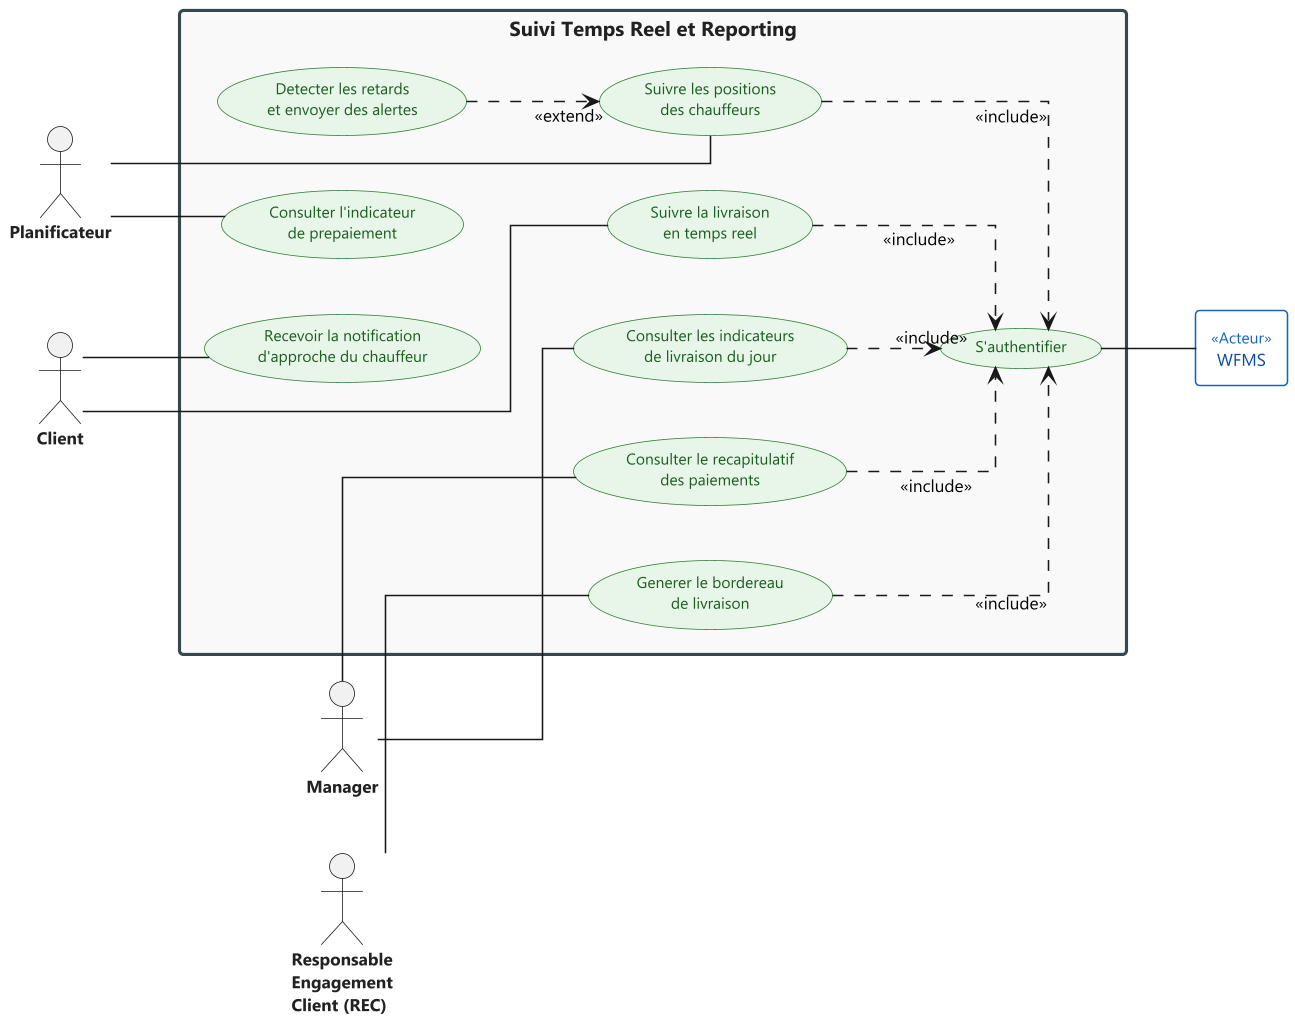
\includegraphics[width=0.9\textwidth, height=0.85\textheight, keepaspectratio]{img/diagrammes/sprint_4_usecase_p3}%
}{%
  \fbox{\parbox{0.9\linewidth}{\centering\vspace{4cm}\textit{[img/diagrammes/sprint\_4\_usecase\_p3.png]}\vspace{4cm}}}%
}
\caption{Diagramme de cas d'utilisation du Sprint~4 --- Partie~3}
\label{fig:cas-utilisation-sp4-p3}
\end{figure}

\subsection{Description textuelle}

\captionsetup[longtable]{justification=centering}
\setlength{\arrayrulewidth}{1pt}
\begin{longtable}{|p{4cm}|p{11cm}|}
\hline
\rowcolor{headerbg}
\textbf{Élément} & \textbf{Description} \\
\hline
\textbf{Titre} & Confirmer une livraison \\
\hline
\textbf{Acteurs} & Chauffeur, Responsable des Engagements Clients (REC), Planificateur \\
\hline
\textbf{Objectif} & Permettre au Chauffeur de valider la remise de la marchandise avec preuves numériques depuis l'application mobile, et au Planificateur/Manager de suivre l'exécution en temps réel depuis l'interface web. \\
\hline
\textbf{Précondition} & La livraison est au statut EN\_COURS. Le paiement est validé (ou le mode est prépayé). Le Chauffeur est connecté à l'app mobile. \\
\hline
\textbf{Postcondition} & La livraison passe au statut LIVRÉE. La preuve est archivée (chiffrement AES-256, 5 ans). Le client et le REC sont notifiés. \\
\hline
\textbf{Scénario nominal} &
\begin{enumerate}[start=1, label=\arabic*.]
    \item Le Chauffeur ouvre la livraison depuis l'app mobile et clique sur « Confirmer ».
    \item Le client signe sur l'écran tactile ; la signature est encodée en base64.
    \item Le Chauffeur prend des photos géolocalisées horodatées de la marchandise livrée.
    \item Le Chauffeur valide les articles remis et détecte tout écart avec la commande.
    \item Le système enregistre la preuve et passe la livraison au statut LIVRÉE.
    \item Le Planificateur voit la mise à jour en temps réel sur la carte GPS et le tableau de bord KPI.
    \item Le REC génère le bordereau de livraison depuis l'interface web.
\end{enumerate} \\
\hline
\textbf{Scénario alternatif} &
\begin{enumerate}[start=1, label=\arabic*.]
    \item Client absent : le Chauffeur sélectionne le motif « Client absent » ; statut passe à ÉCHOUÉE.
    \item Article non conforme : une alerte est générée et envoyée au REC.
    \item Mode de paiement non validé : la confirmation est bloquée jusqu'à l'approbation REC.
    \item Livraison échouée non traitée : le Planificateur la reprogramme en priorité le lendemain.
\end{enumerate} \\
\hline
\caption{Description textuelle --- Confirmer une livraison (Sprint 4)}
\end{longtable}
\setlength{\arrayrulewidth}{0.4pt}

\subsection{Diagramme de classes}

\newpage
\thispagestyle{empty}
\begin{landscape}
\begin{figure}[H]
\centering
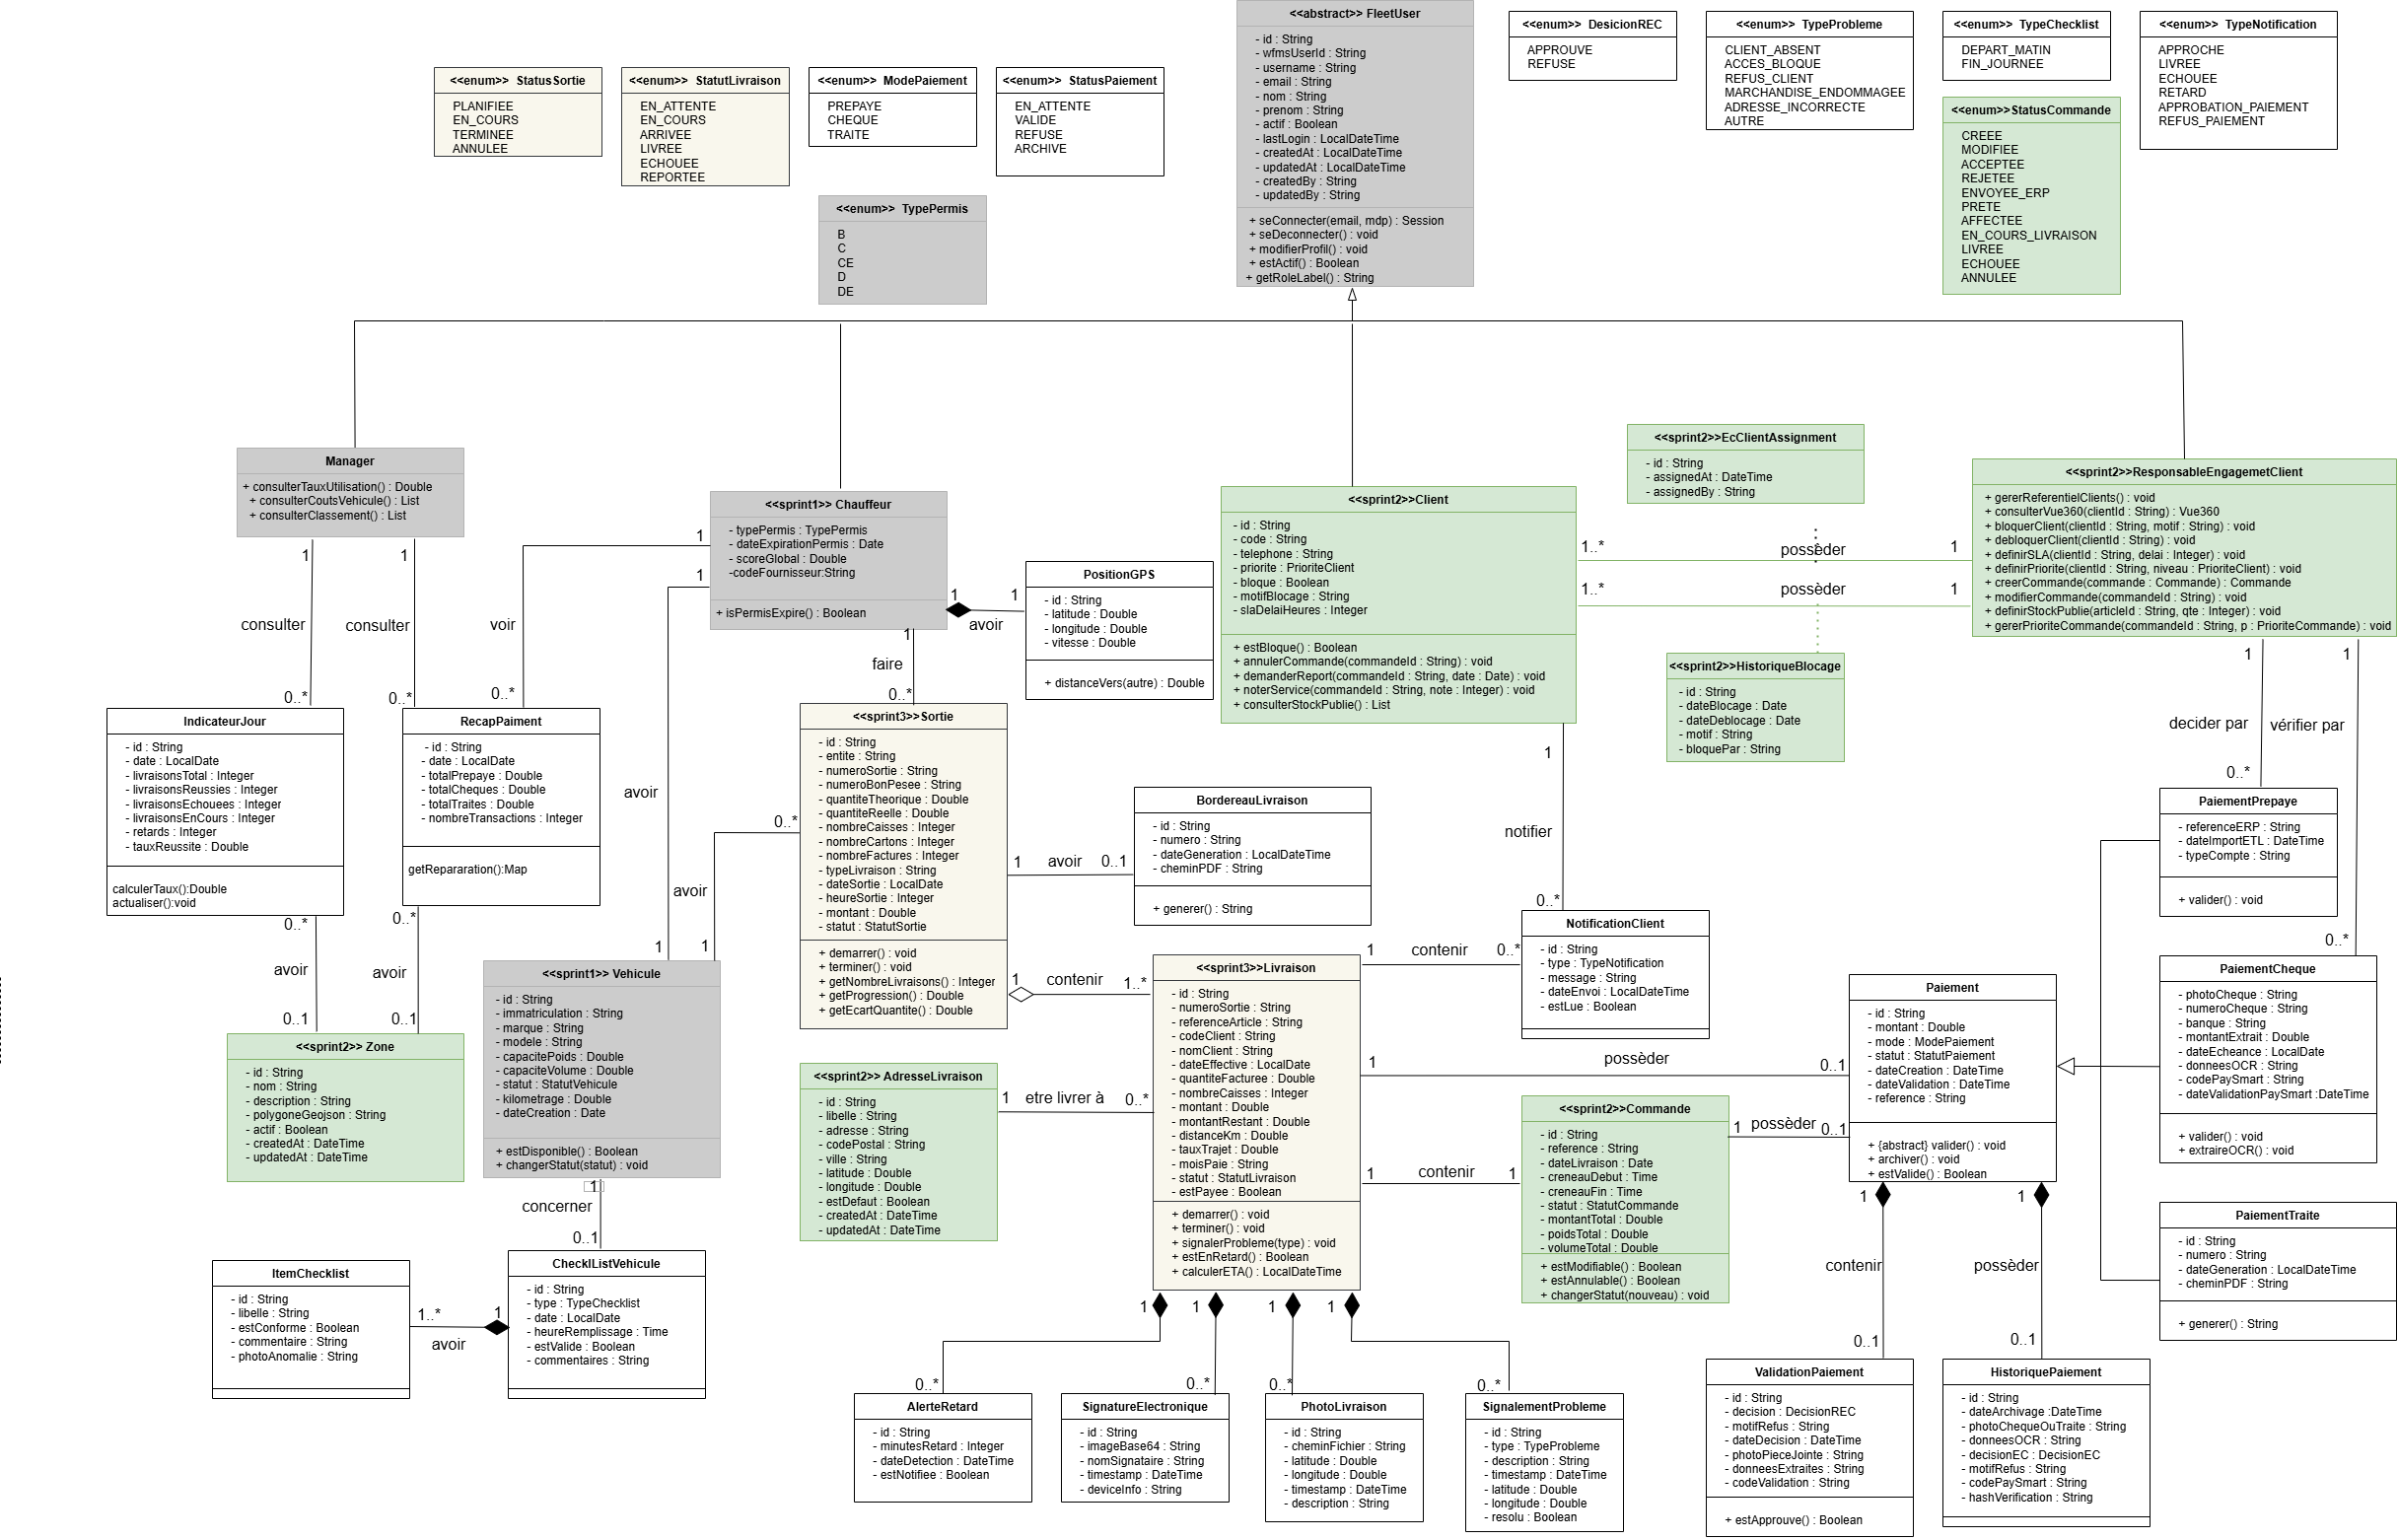
\includegraphics[width=\linewidth, height=0.95\textheight, keepaspectratio]{img/diagrammes/sprint_4_classes}
\caption{Diagramme de classes du Sprint 4}
\label{fig:diag-classes-sp4}
\end{figure}
\end{landscape}

% =============================================================
\section{Réalisation}
% =============================================================

\subsection{Suivi GPS en temps réel et tableau de bord de pilotage}

Le Sprint~4 marque le début de l'exécution terrain. Le Planificateur suit en temps réel la position de tous les chauffeurs actifs sur une carte Leaflet, mise à jour toutes les 30~secondes via WebSocket (STOMP/SockJS). Un service planifié détecte automatiquement les retards dépassant 15~minutes et déclenche des alertes visuelles sur l'interface. Le Manager dispose d'un tableau de bord KPI journalier affichant le taux de réussite, le nombre de livraisons en cours et les alertes actives. Le Client reçoit une notification lorsque le Chauffeur est à moins de dix minutes de son adresse.

\begin{figure}[H]
\centering
\IfFileExists{img/capture/web/sp4_tracking_kpi_composite.png}{%
  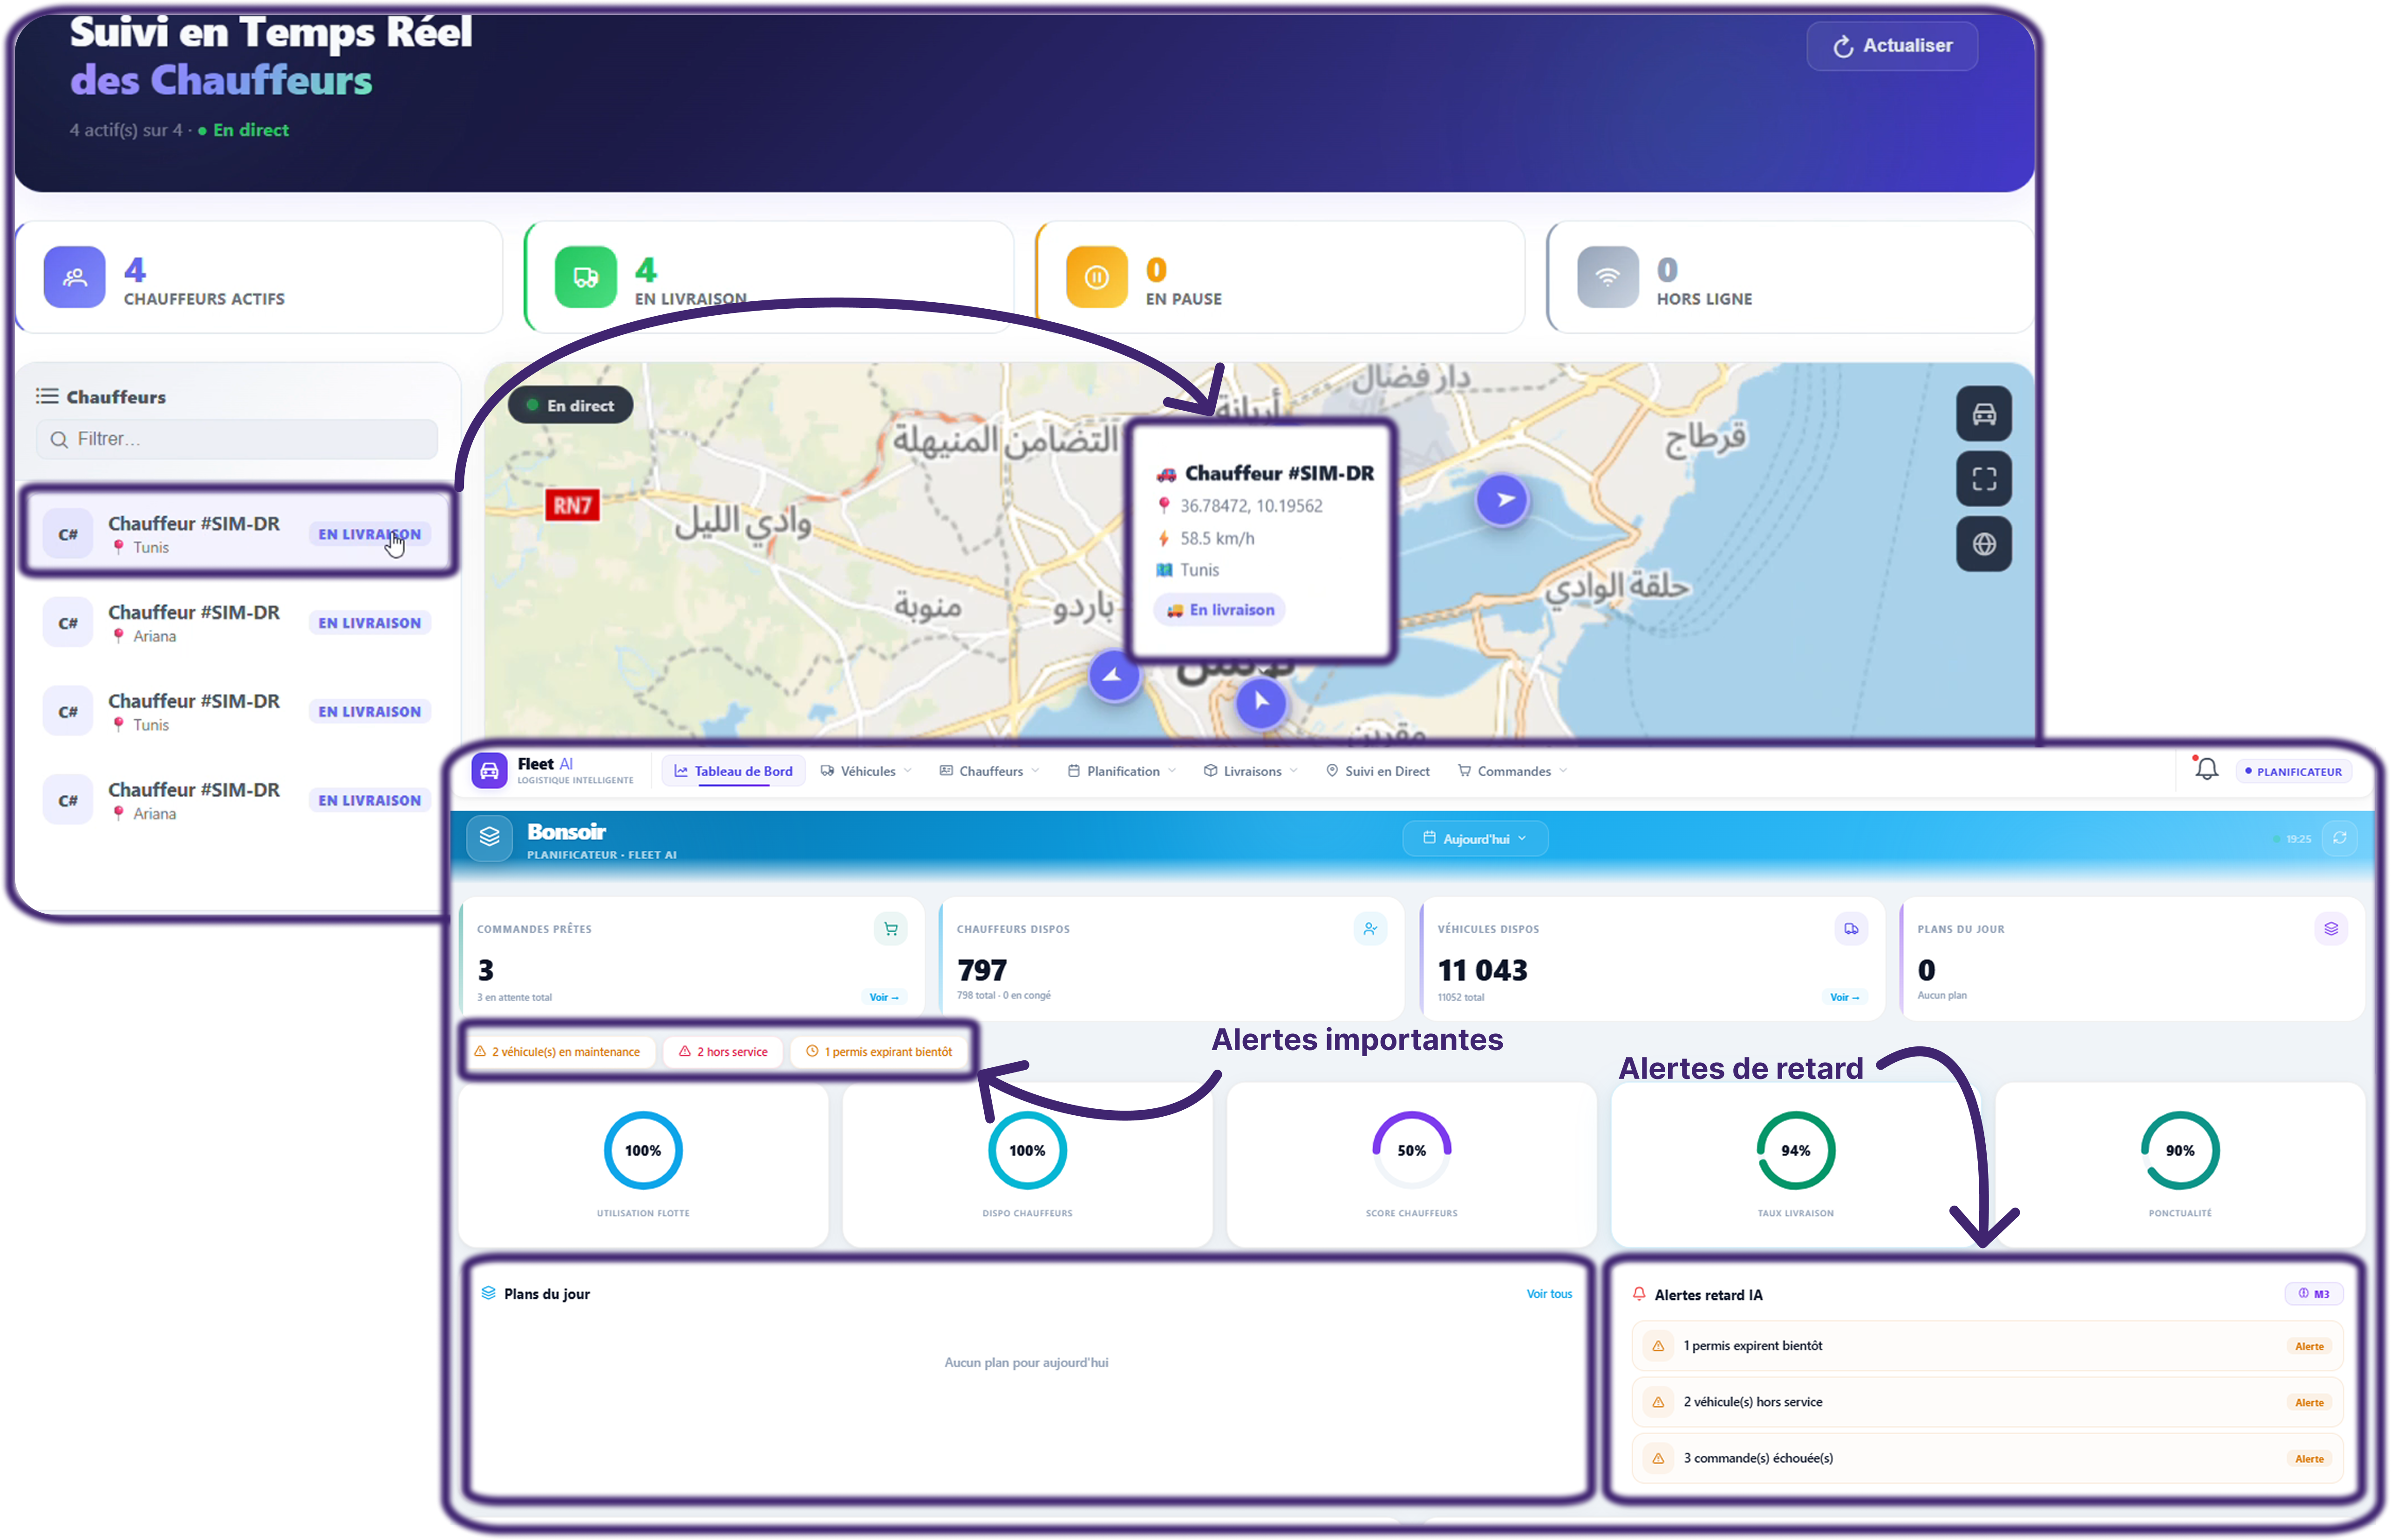
\includegraphics[width=\linewidth, keepaspectratio]{img/capture/web/sp4_tracking_kpi_composite}%
}{%
  \fbox{\parbox{0.9\linewidth}{\centering\vspace{4cm}\textit{[img/sp4\_tracking\_kpi\_composite]}\vspace{4cm}}}%
}
\caption{Carte GPS WebSocket, alertes retard et KPI journalier}
\label{fig:sp4-tracking}
\end{figure}

\subsection{Gestion des trois modes de paiement}

Le système prend en charge trois modes de paiement distincts, gérés exclusivement depuis l'interface web par le REC. Le mode \textbf{Prépayé} autorise la livraison automatiquement grâce au statut importé de l'ERP~: aucune action manuelle n'est requise. Le mode \textbf{Chèque} implique une capture OCR automatisée (GrepSys) par le Chauffeur, suivie d'une saisie dans PaySmart par le REC et d'une validation SMS envoyée au client. Le mode \textbf{Traite} requiert la photo de la traite et une décision explicite du REC (APPROUVÉ ou REFUSÉ avec motif obligatoire), tracée dans l'historique de paiement.

\begin{figure}[H]
\centering
\IfFileExists{img/capture/web/sp4_payment_composite.png}{%
  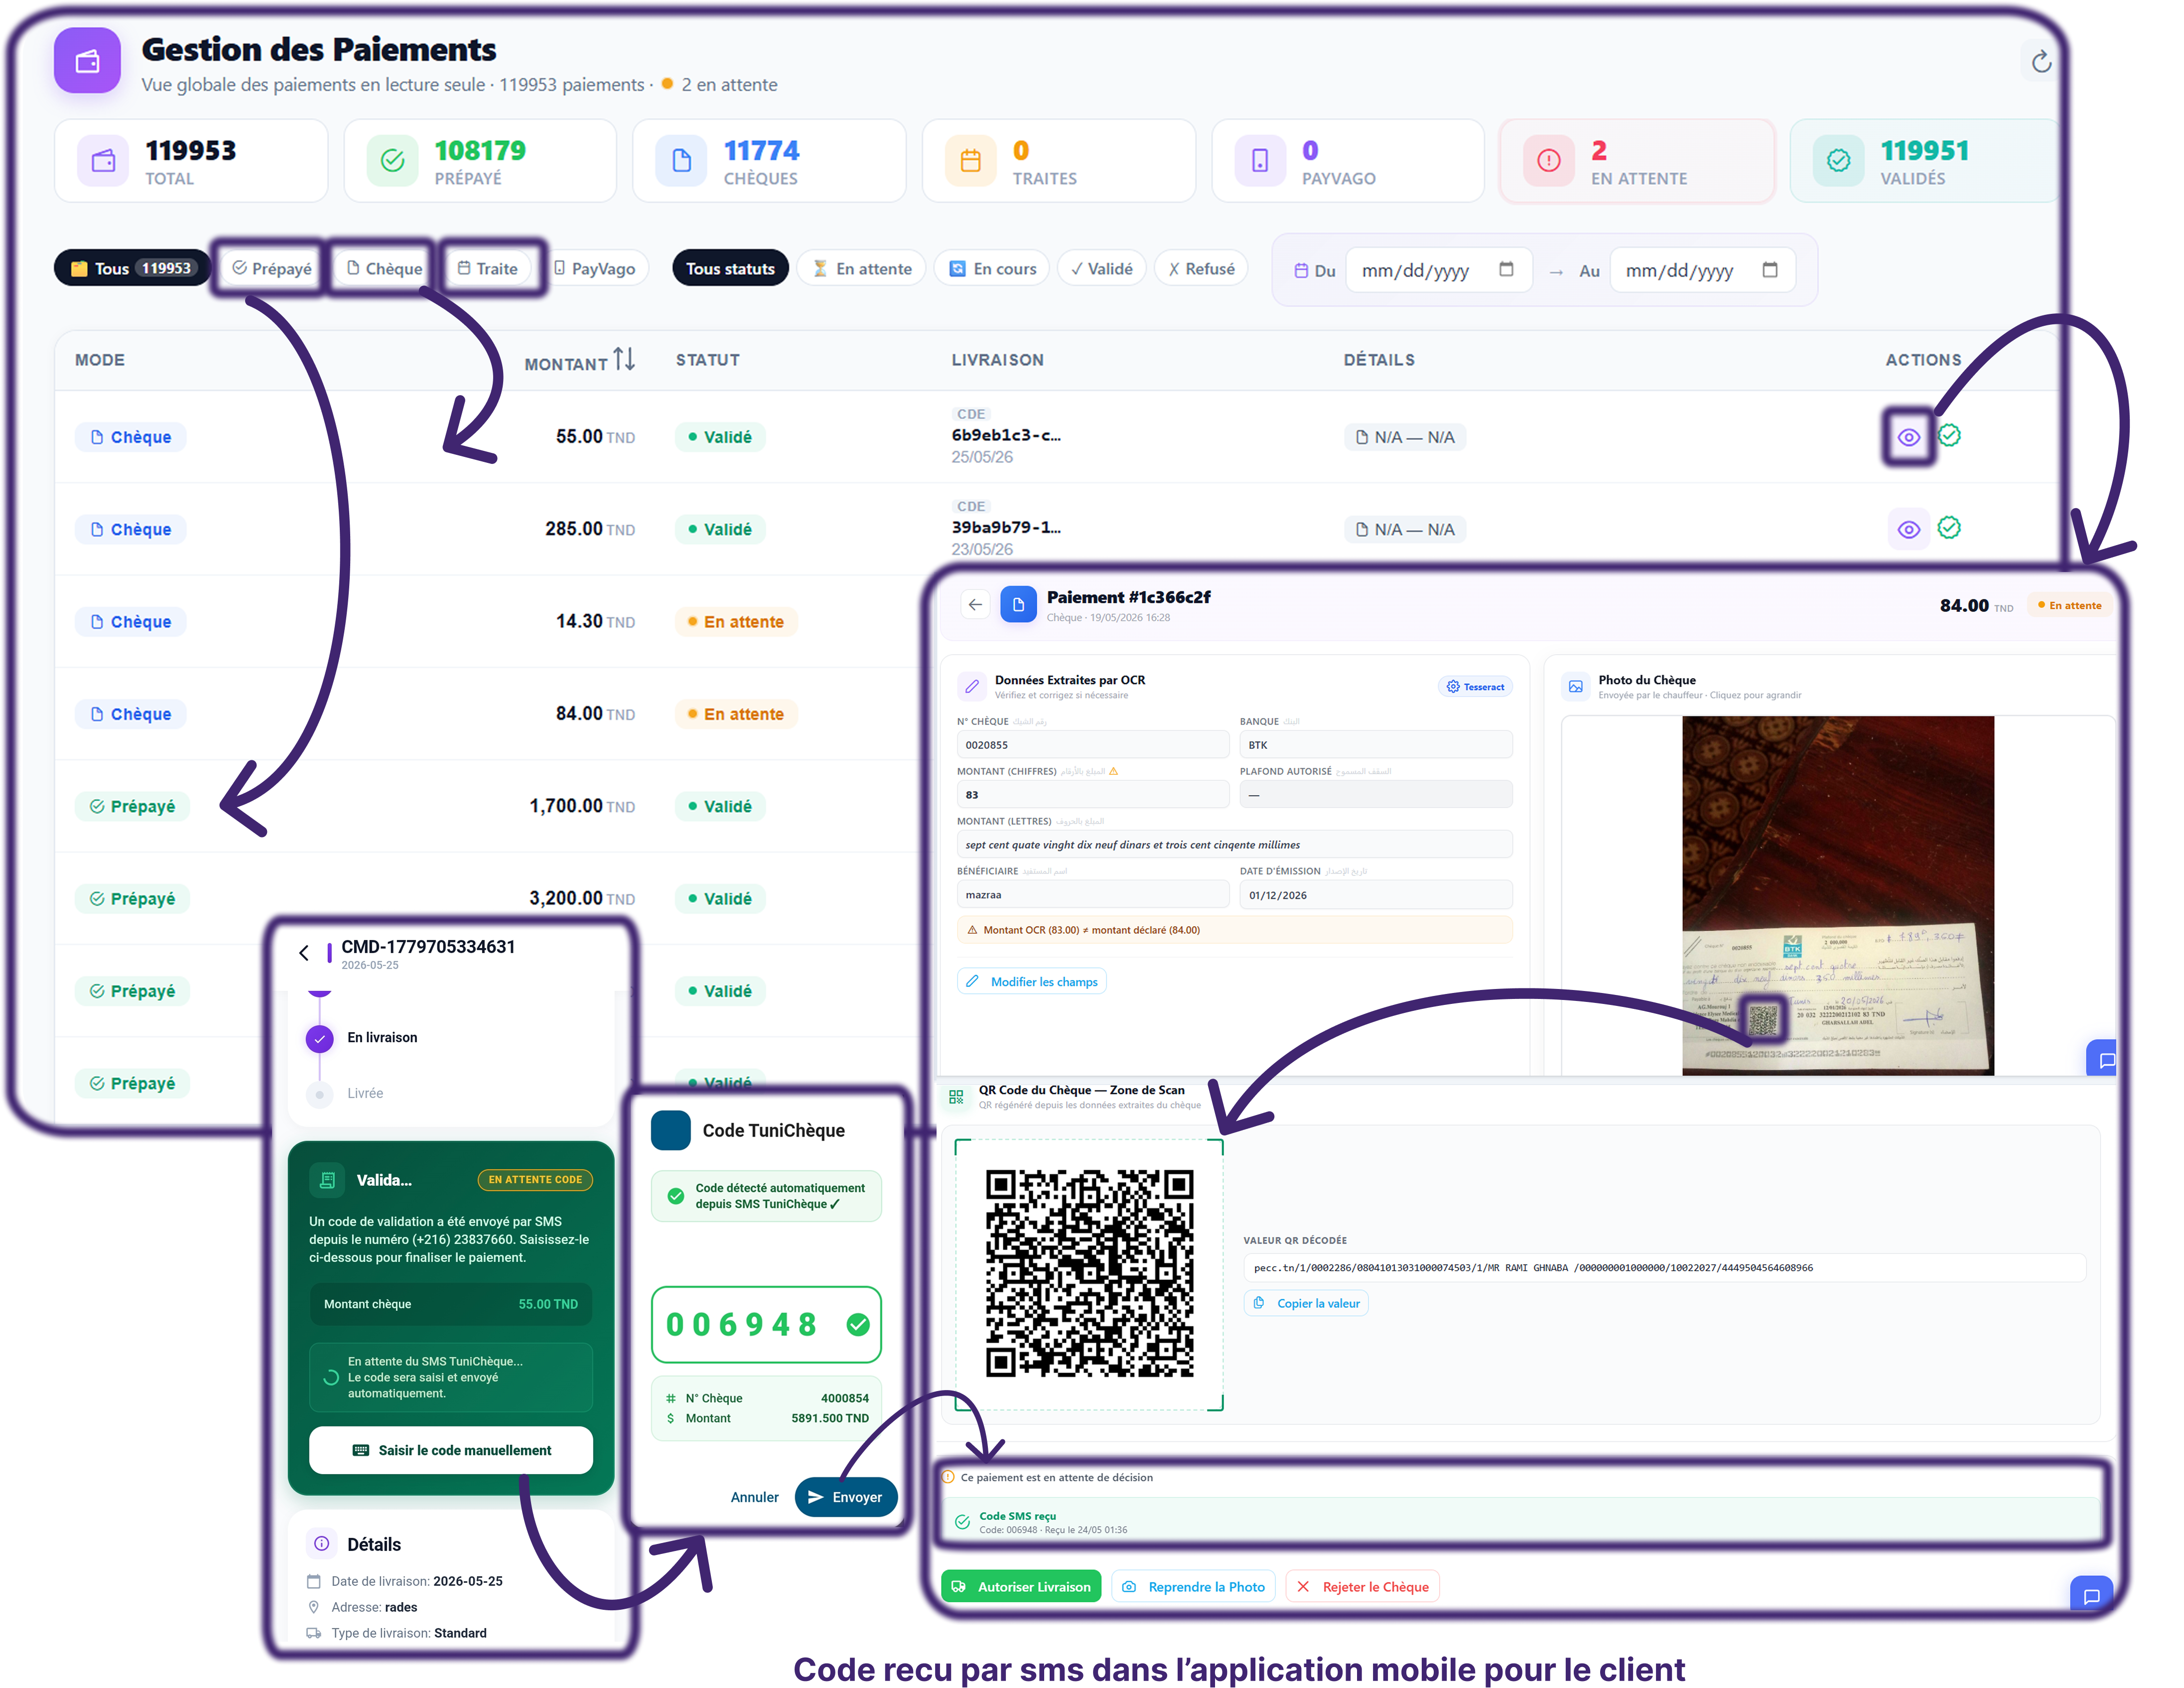
\includegraphics[width=\linewidth, keepaspectratio]{img/capture/web/sp4_payment_composite}%
}{%
  \fbox{\parbox{0.9\linewidth}{\centering\vspace{4cm}\textit{[img/sp4\_payment\_composite]}\vspace{4cm}}}%
}
\caption{Paiements : prépayé, chèque OCR et décision traite REC}
\label{fig:sp4-payments}
\end{figure}

\subsection{Gestion des livraisons échouées et reprogrammation}

En cas d'impossibilité de livrer, le Chauffeur signale le problème sur l'application mobile (CLIENT\_ABSENT, ACCES\_BLOQUE, REFUS\_CLIENT, MARCHANDISE\_ENDOMMAGEE, ADRESSE\_INCORRECTE). Le statut passe immédiatement à ÉCHOUÉE et une notification est envoyée au Planificateur et au REC. Depuis l'interface web, le Planificateur consulte la liste des livraisons échouées du jour et peut les reprogrammer en priorité le lendemain (J+1) avec réaffectation automatique.

\begin{figure}[H]
\centering
\IfFileExists{img/capture/web/sp4_reclamations_composite.png}{%
  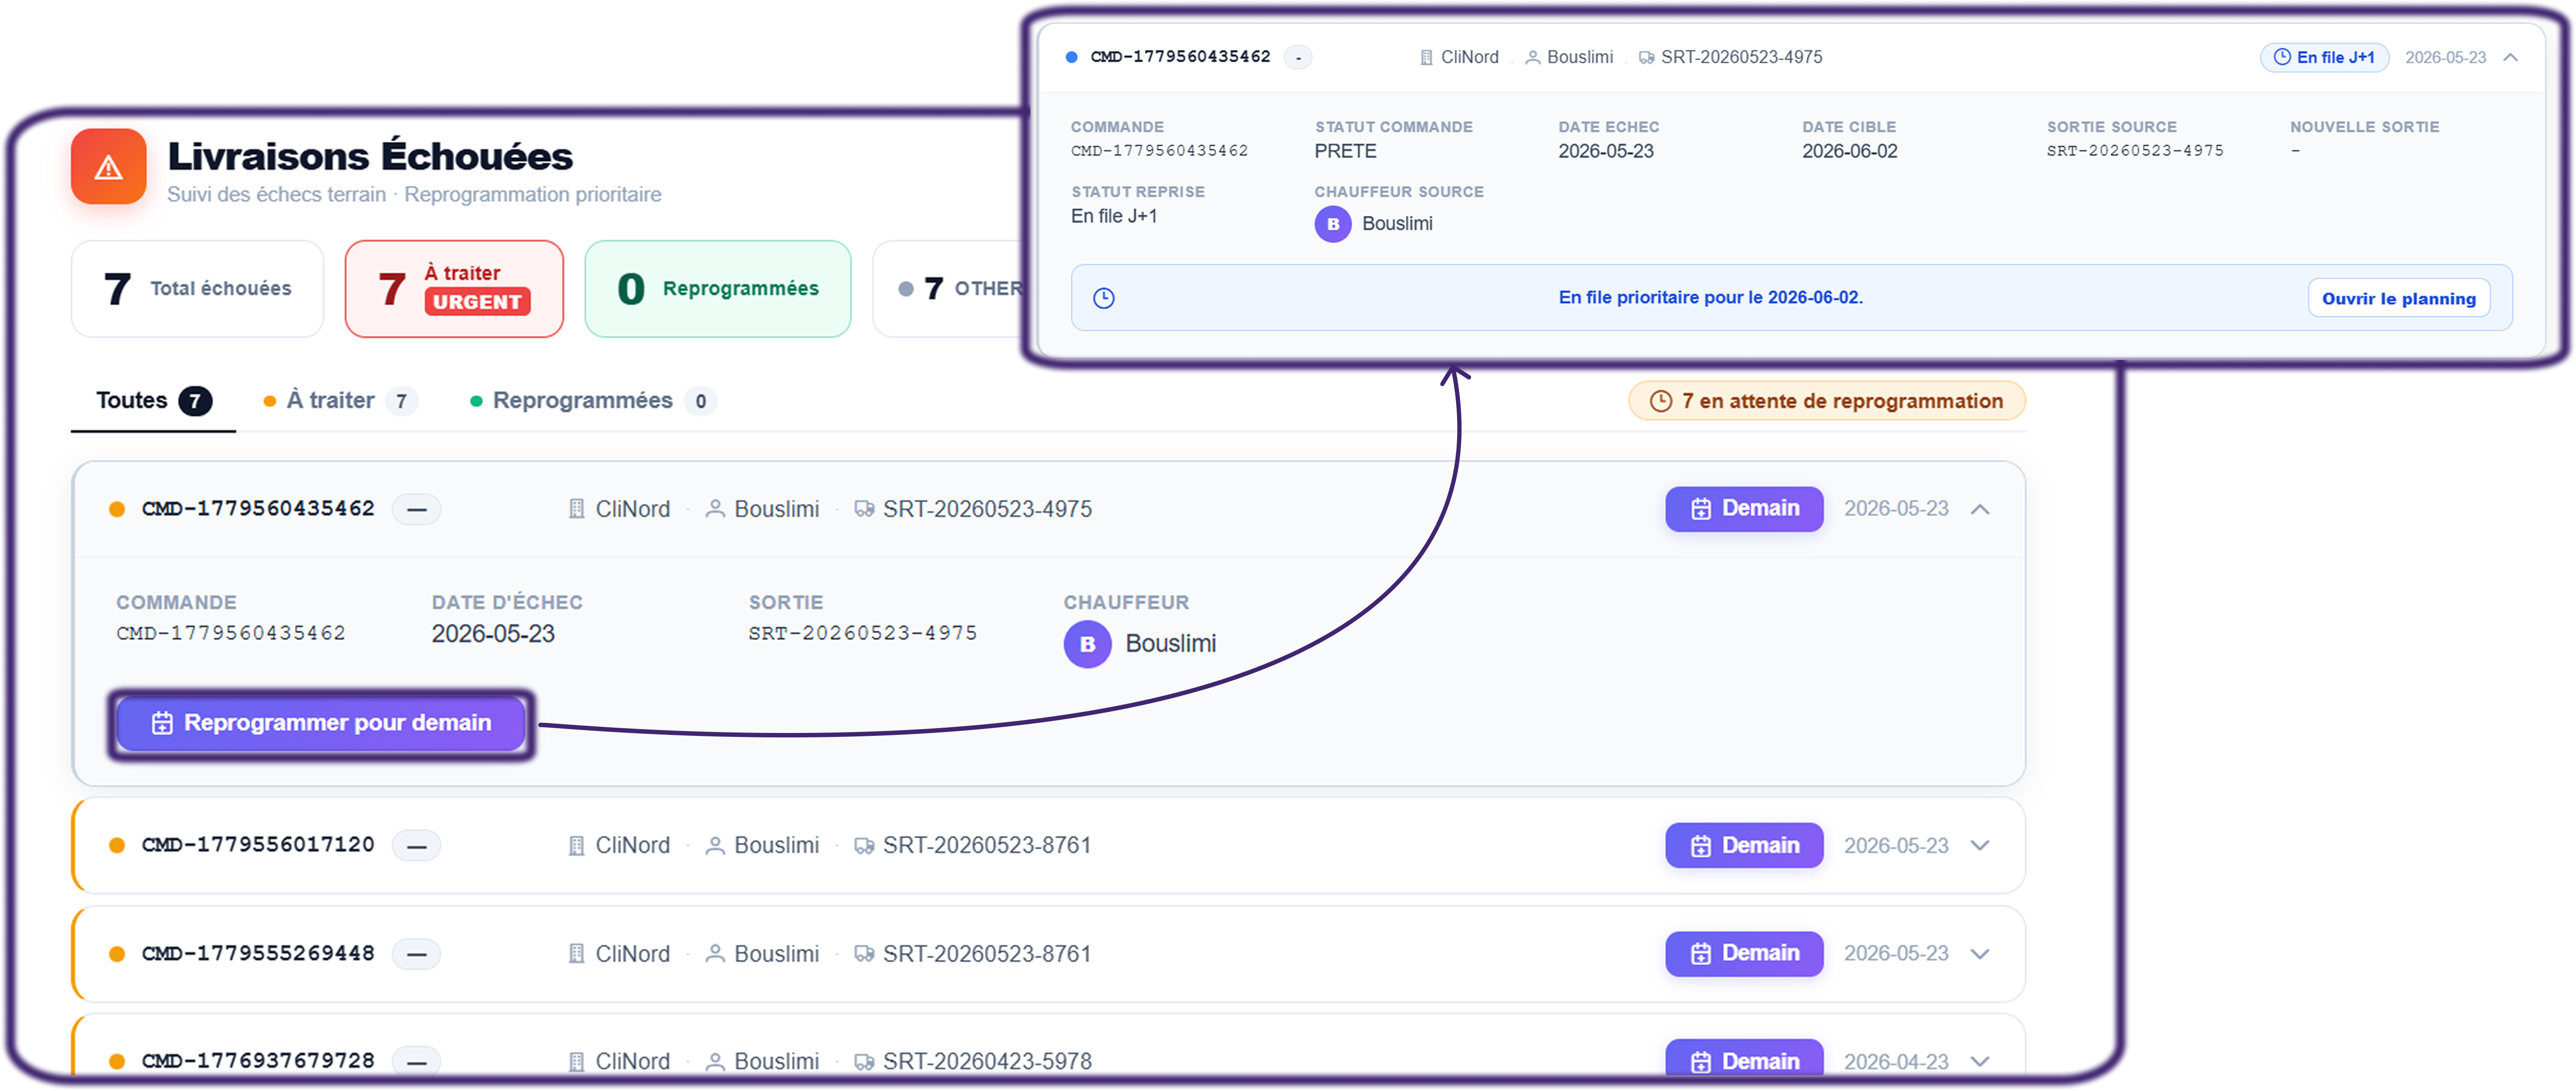
\includegraphics[width=\linewidth, keepaspectratio]{img/capture/web/sp4_reclamations_composite}%
}{%
  \fbox{\parbox{0.9\linewidth}{\centering\vspace{4cm}\textit{[img/sp4\_issues\_composite]}\vspace{4cm}}}%
}
\caption{Livraisons échouées : motifs et reprogrammation J+1}
\label{fig:sp4-issues}
\end{figure}

\subsection{Bordereaux de livraison et clôture de tournée}

En fin de journée, le REC génère depuis l'interface web un bordereau de livraison pour chaque tournée, récapitulant les montants encaissés par mode de paiement (espèces, chèque, traite) et le statut de chaque livraison (LIVRÉE / ÉCHOUÉE / REPORTÉE). Ce bordereau sert de document officiel de clôture de tournée. La réconciliation des encaissements par rapport aux commandes planifiées est effectuée automatiquement par le système.

\begin{figure}[H]
\centering
\IfFileExists{img/capture/web/sp4_recap_composite.png}{%
  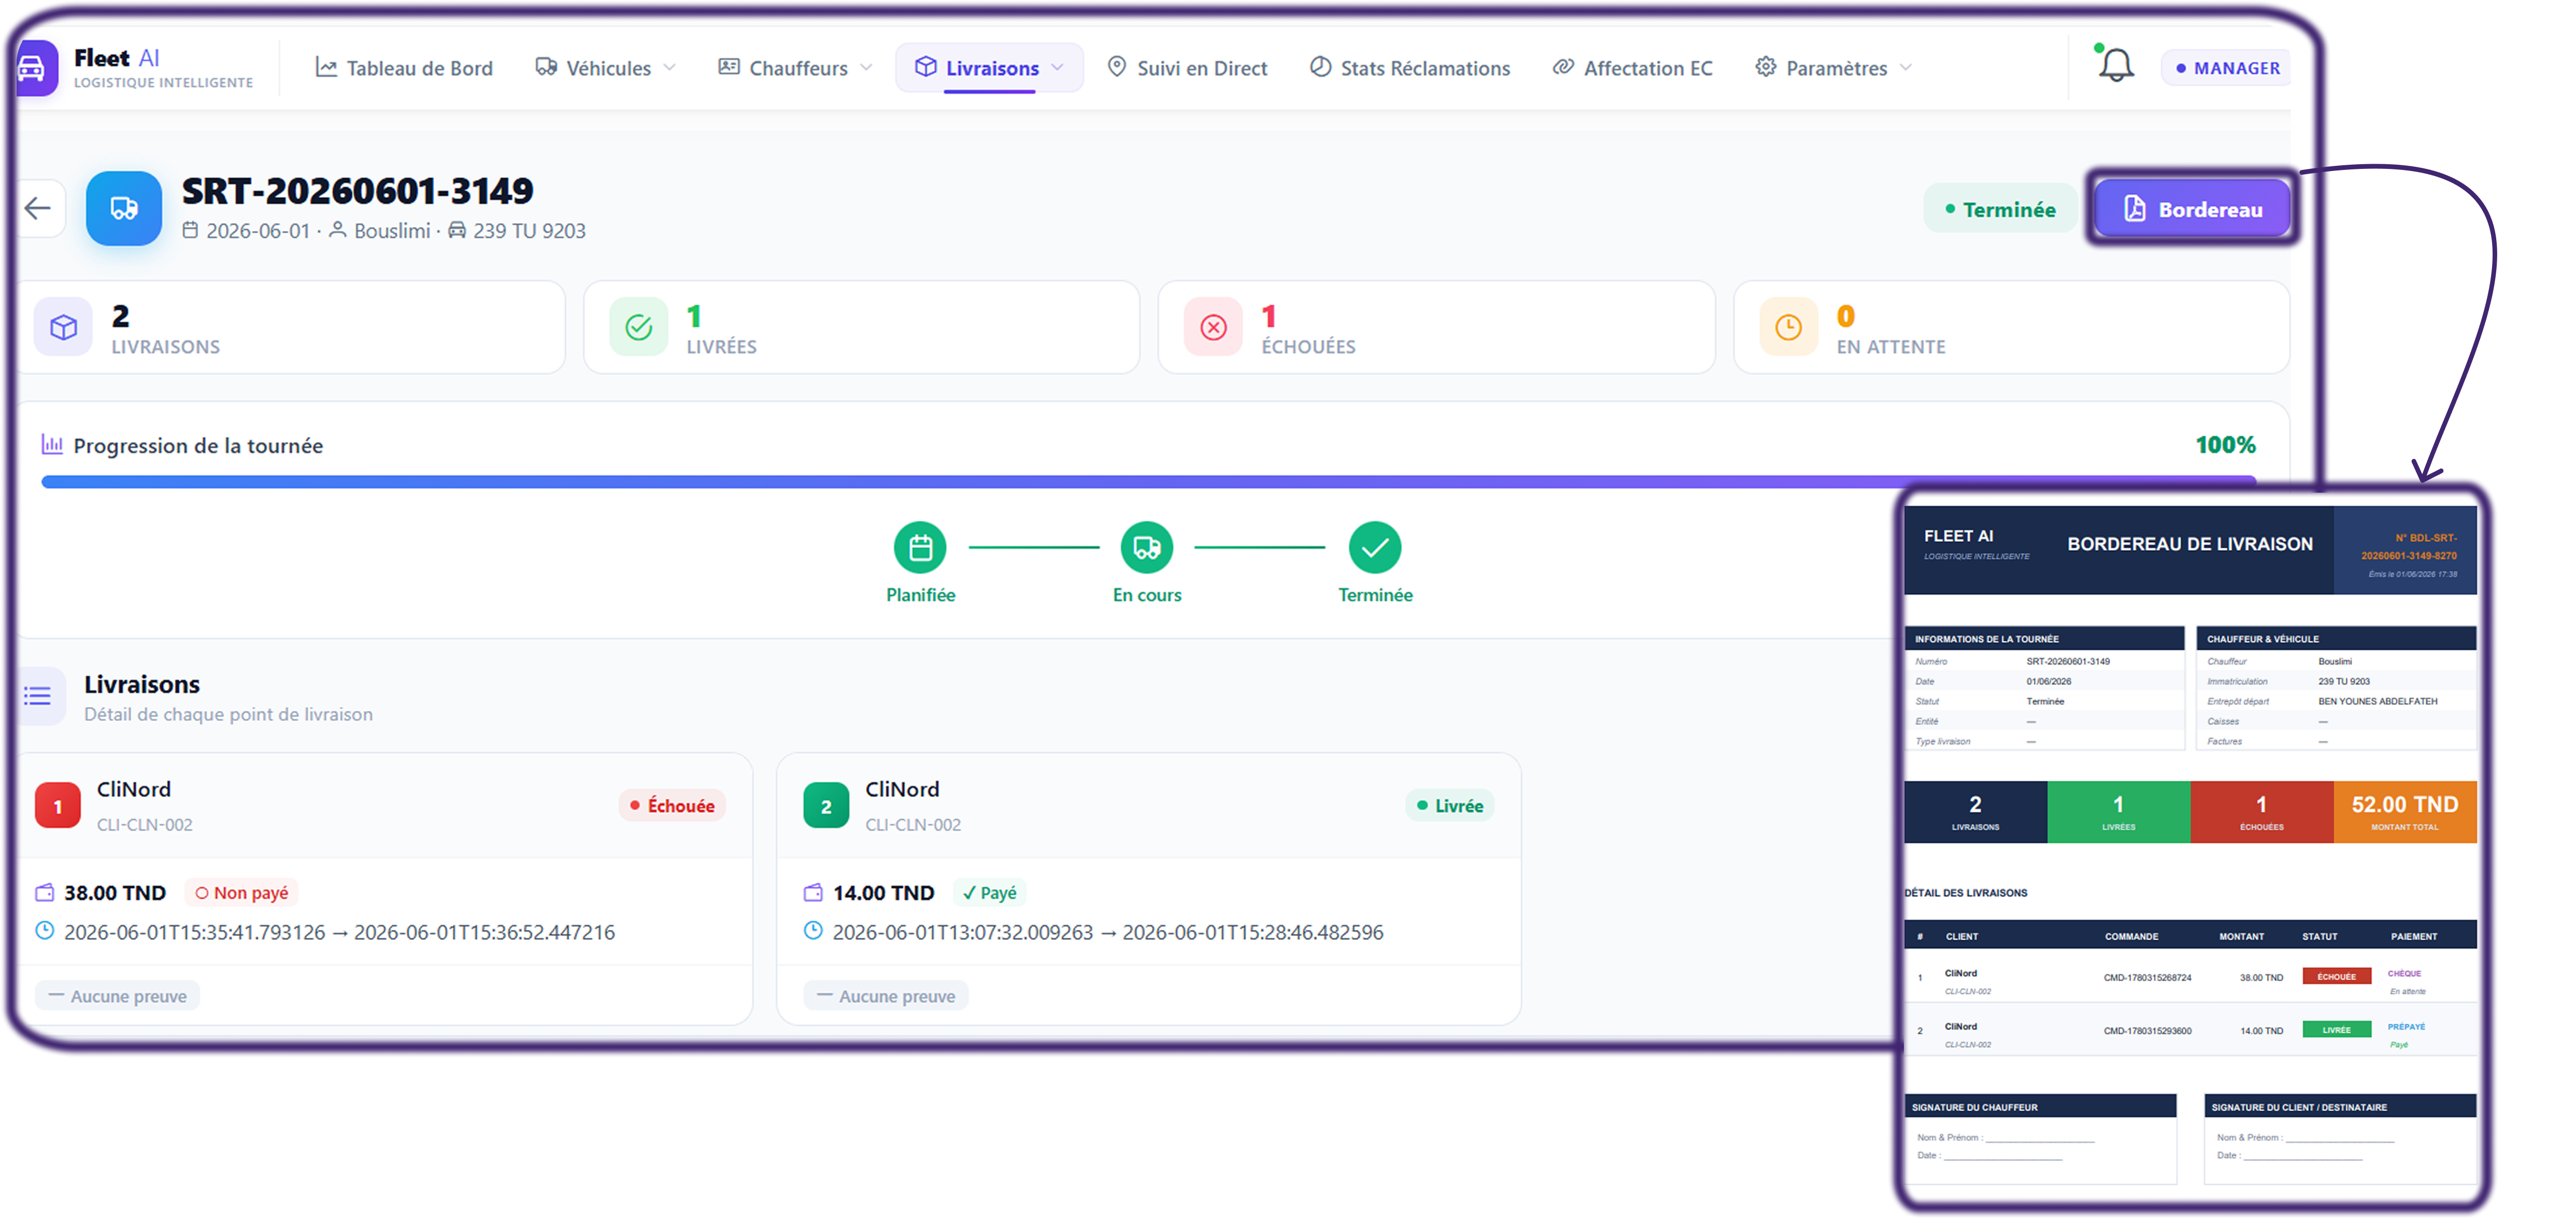
\includegraphics[width=\linewidth, keepaspectratio]{img/capture/web/sp4_recap_composite}%
}{%
  \fbox{\parbox{0.9\linewidth}{\centering\vspace{4cm}\textit{[img/capture/web/sp4\_recap\_composite.png]}\vspace{4cm}}}%
}
\caption{Bordereau de clôture et réconciliation encaissements}
\label{fig:sp4-recap}
\end{figure}

\subsection{Gestion et suivi des réclamations}

Le REC traite les réclamations clients depuis une interface web dédiée, avec visualisation du statut, du délai de traitement et de l'historique des échanges. Si une réclamation reste non traitée après 48~heures, le système l'escalade automatiquement au Manager avec notification. Depuis l'application mobile, le Client peut soumettre une réclamation en sélectionnant la catégorie et la description, et suivre l'état de traitement en temps réel de ses tickets ouverts (Ouvertes / En cours / Résolues).

\begin{figure}[H]
\centering
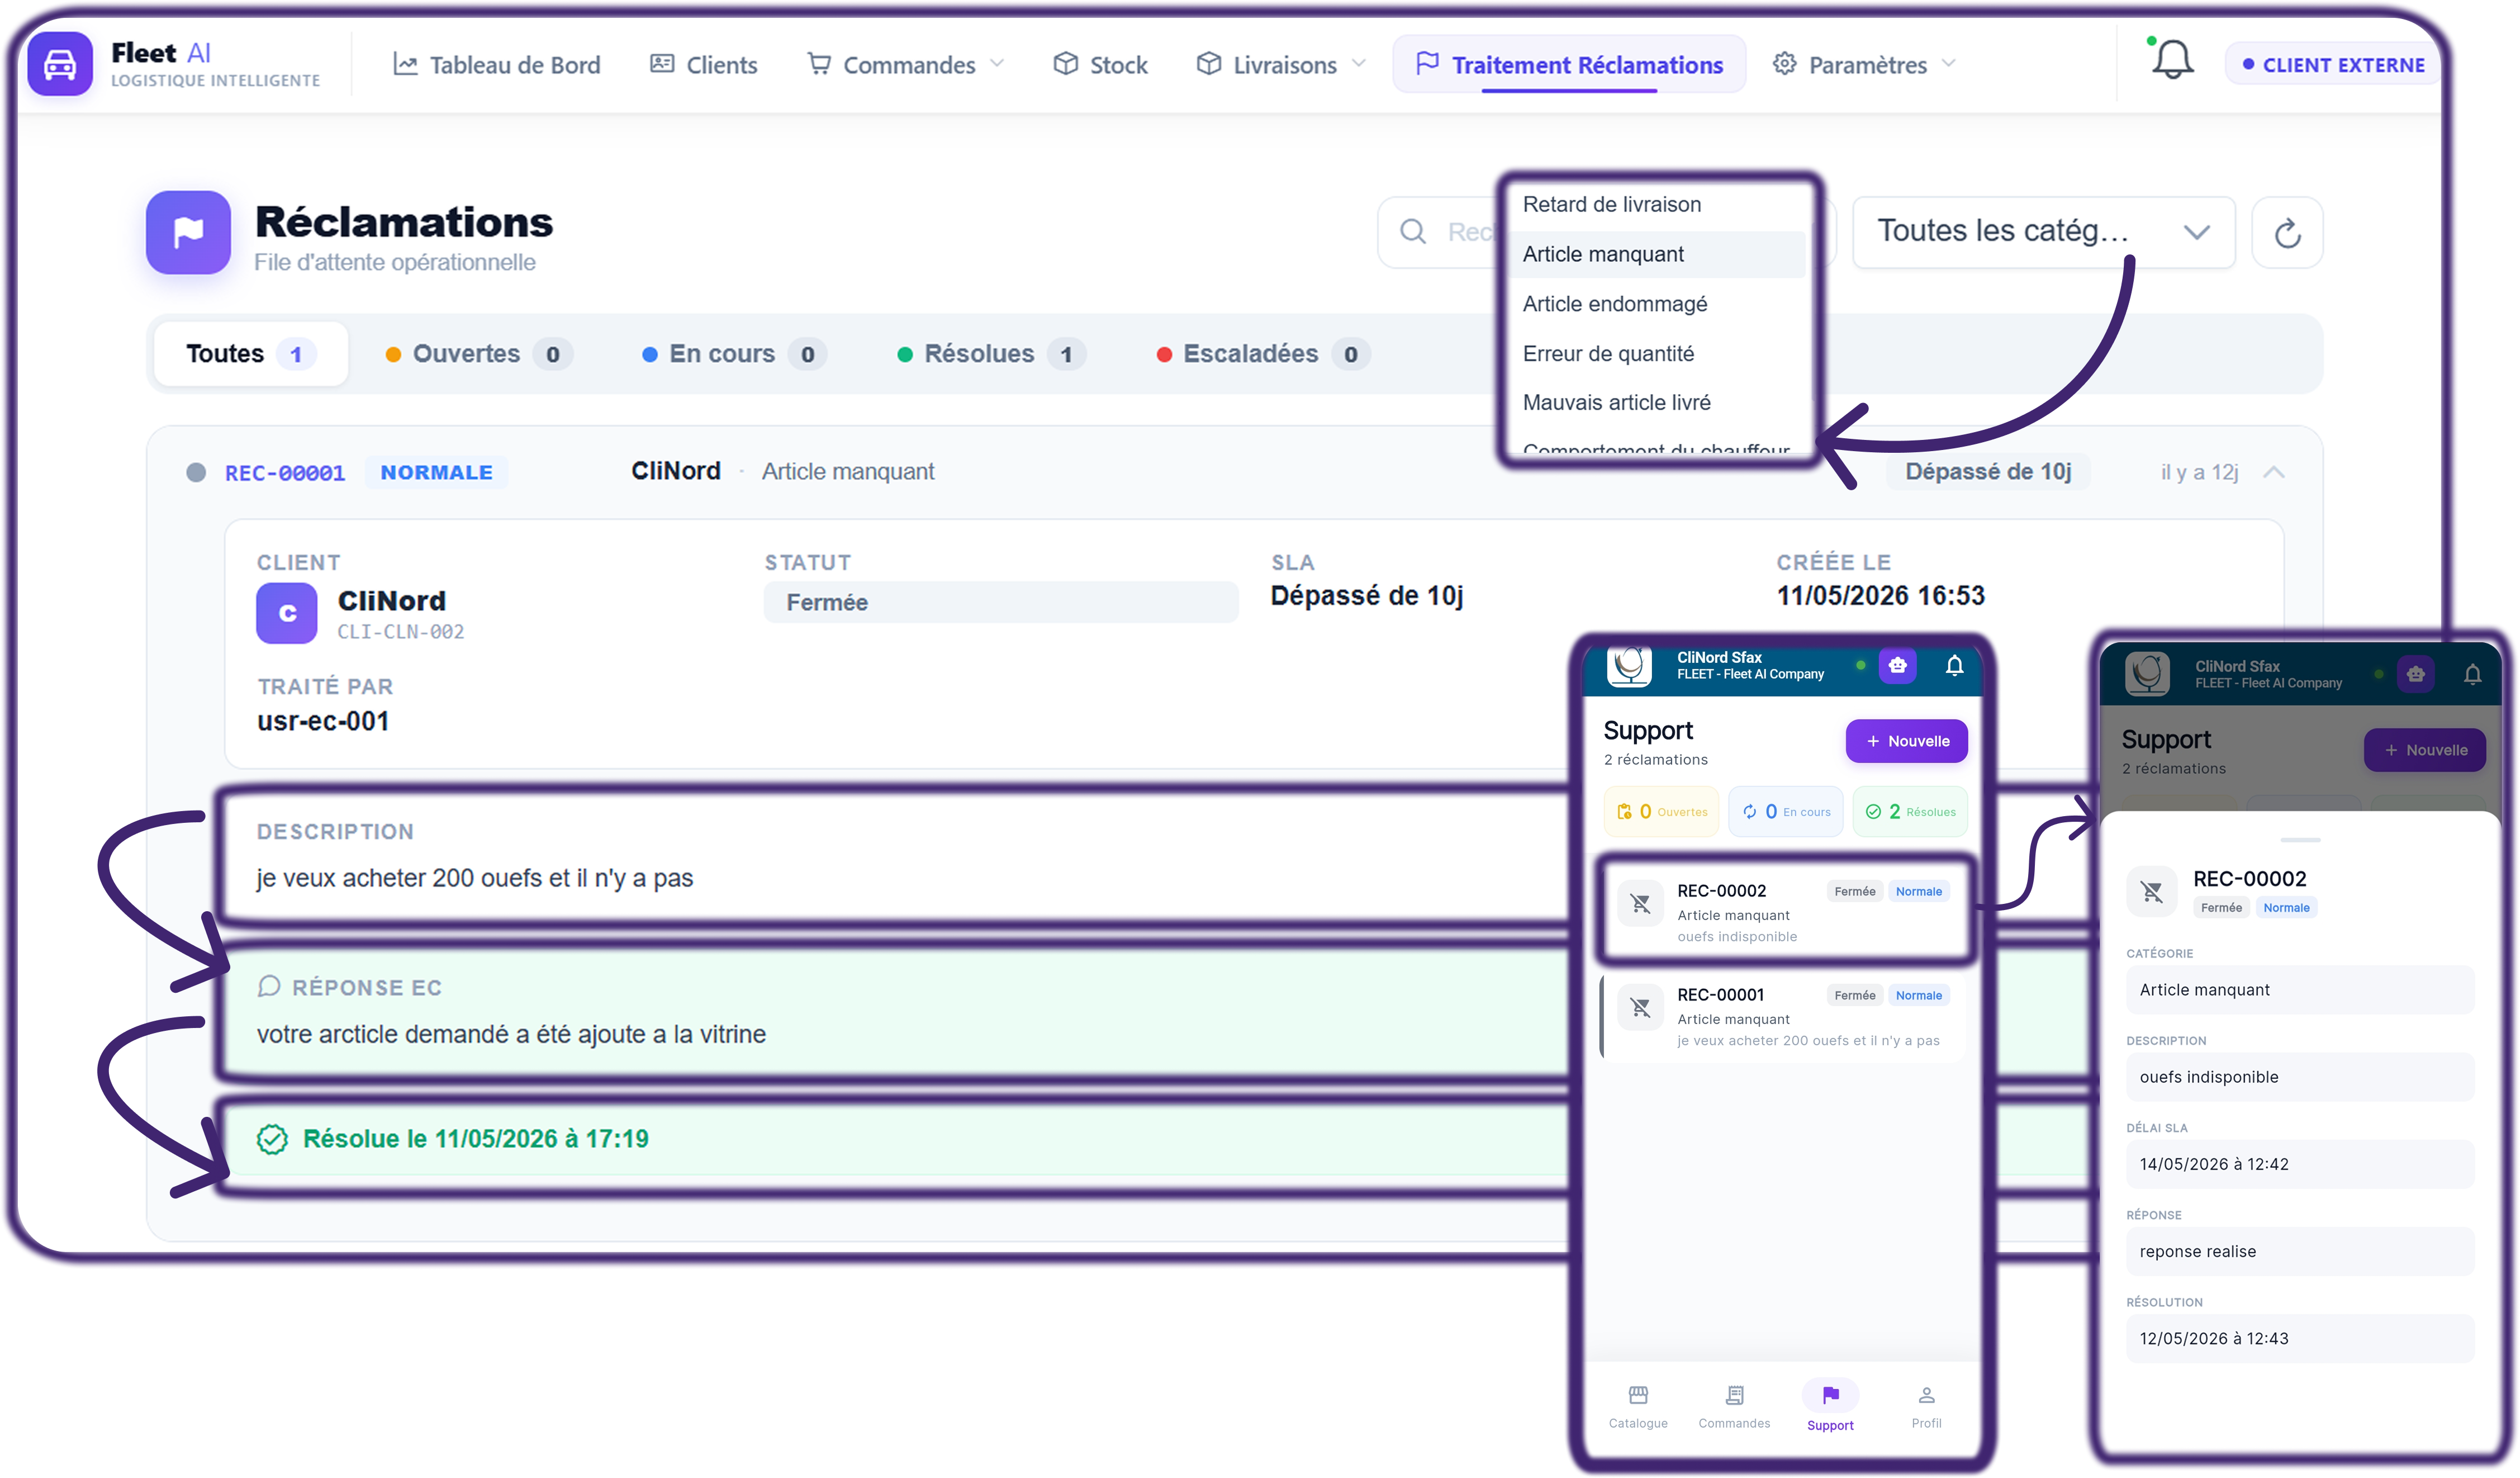
\includegraphics[width=\linewidth, keepaspectratio]{img/capture/mobile/support_client}
\caption{Interface Composite Web et Mobile --- Module Support : liste des réclamations avec statut et priorité (REC-00002, REC-00001), et détail d'un ticket avec catégorie, description, délai SLA, réponse du REC et date de résolution}
\label{fig:sp4-reclamations}
\end{figure}

\subsection{Application mobile Chauffeur --- Démarrage de sortie et checklist}

Avant sa première livraison, le Chauffeur accepte le plan qui lui a été attribué, valide la checklist de contrôle véhicule (niveau d'huile, carburant, rétroviseurs, documents, propreté, chargement sécurisé) puis autorise le suivi GPS en arrière-plan. Une fois la checklist validée, la sortie démarre : le statut passe à \textit{En cours}, la première livraison s'active automatiquement et l'itinéraire complet (578~km, 4 arrêts) est affiché sur la carte TomTom.

\begin{figure}[H]
\centering
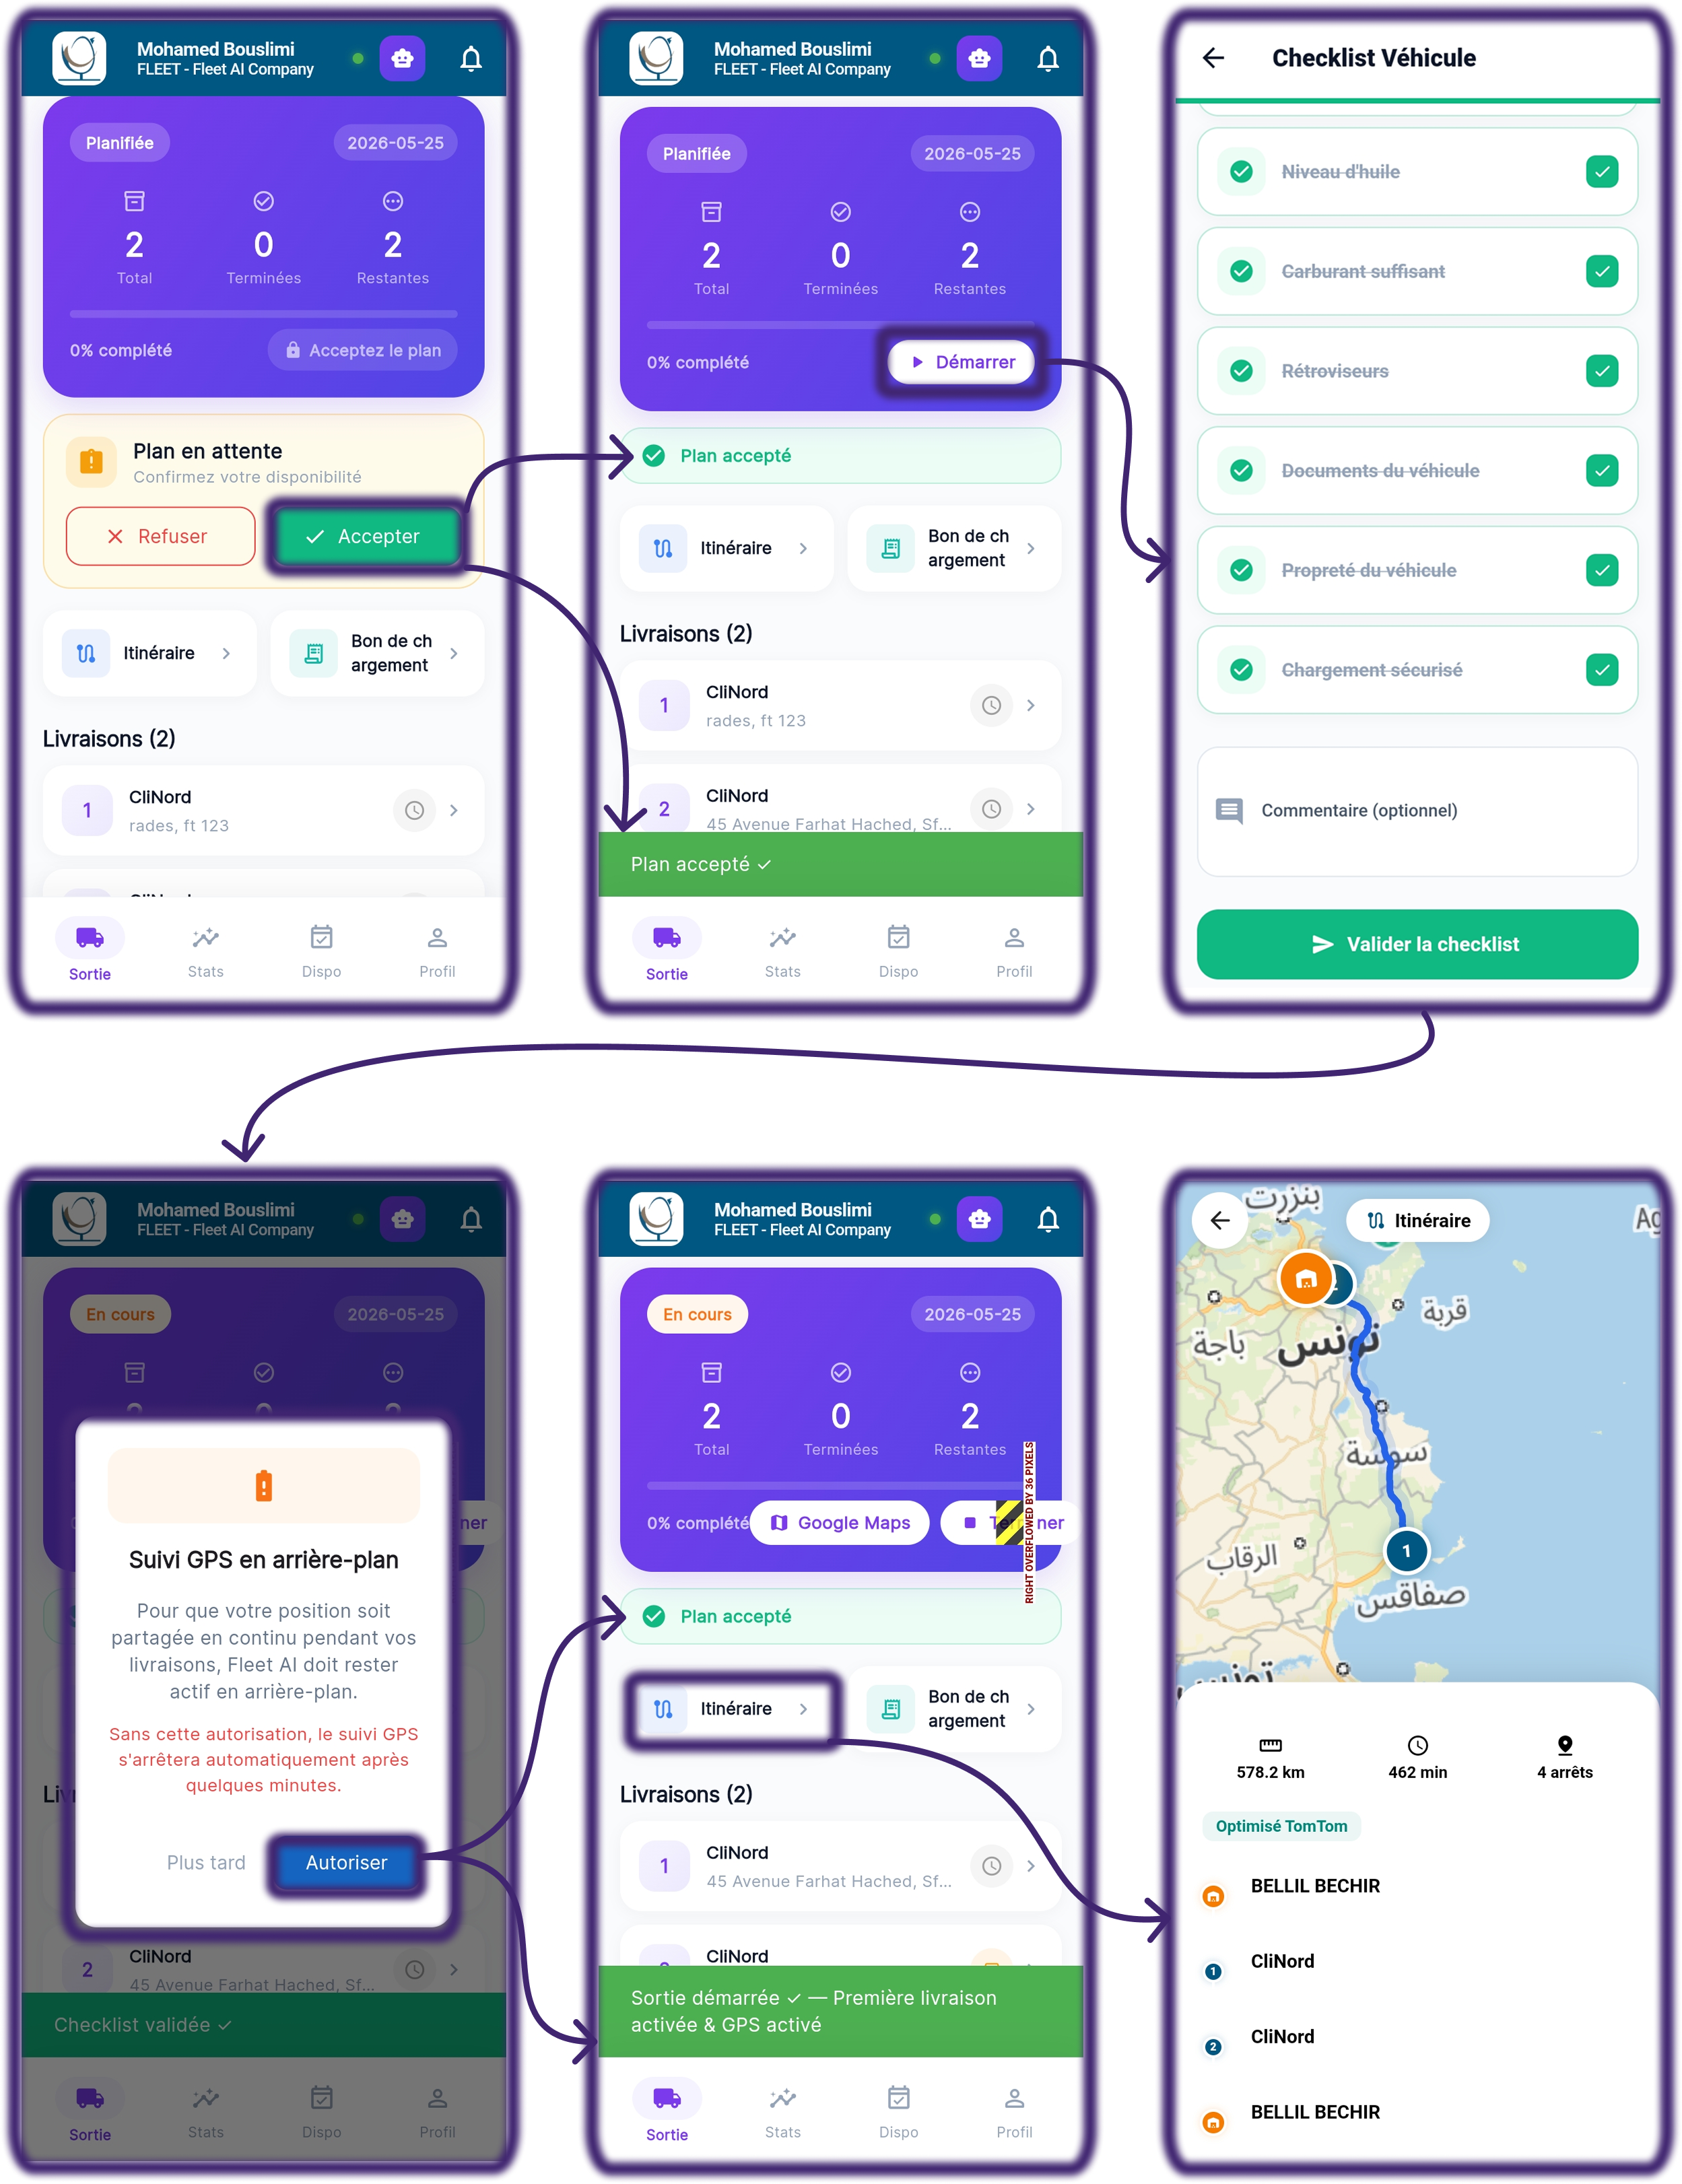
\includegraphics[width=\linewidth, keepaspectratio]{img/capture/mobile/debut_livraison_chauffeur}
\caption{Application mobile Chauffeur --- Démarrage de la sortie : (1)~plan en attente, acceptation, (2)~plan accepté avec bouton Démarrer, (3)~checklist véhicule complète, (4)~autorisation GPS arrière-plan, (5)~sortie démarrée avec activation livraison et (6)~itinéraire optimisé sur carte}
\label{fig:sp4-start}
\end{figure}

\subsection{Application mobile Chauffeur --- Finalisation et paiement de livraison}

A l'arrivée chez le client, le chauffeur signale son arrivée (ou elle est détectée automatiquement par le système GPS quand il entre dans le périmètre de l'adresse). Il consulte le bon de livraison PDF généré automatiquement, prend une photo de la marchandise remise, puis capture le paiement selon le mode indiqué (ici : chèque). L'écran de capture du chèque lui permet de photographier le titre et d'envoyer le montant au REC pour validation. La photo est transmise en temps réel et la livraison passe au statut LIVRÉE après confirmation.

\begin{figure}[H]
\centering
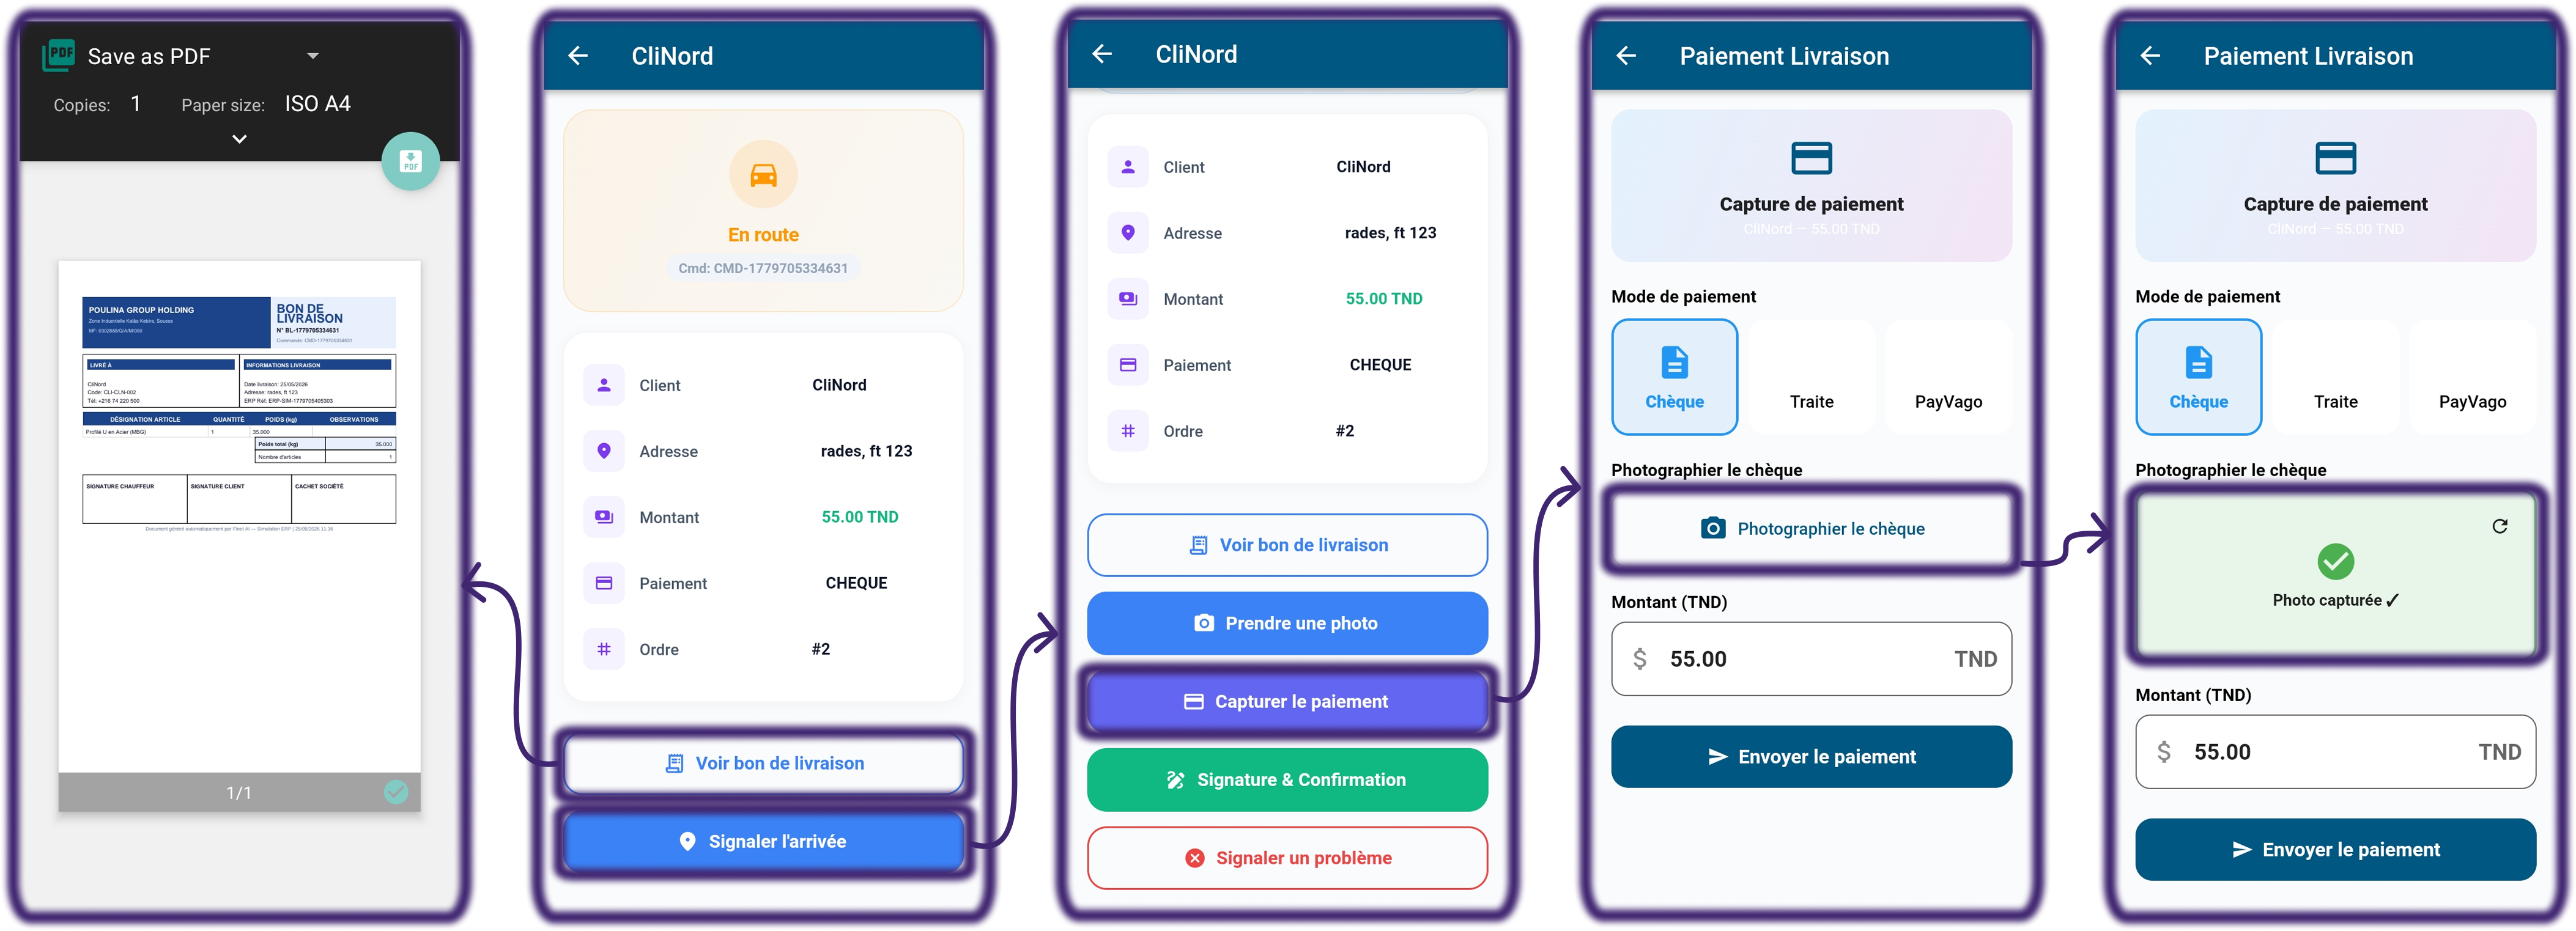
\includegraphics[width=\linewidth, keepaspectratio]{img/capture/mobile/finaliser_livraison_chauffeur}
\caption{Application mobile Chauffeur --- Finalisation de livraison : bon de livraison PDF, signalement d'arrivée, actions terrain (voir bon, prendre photo, capturer paiement, signature, signaler problème), capture du chèque avec photo et envoi au REC}
\label{fig:sp4-proof}
\end{figure}

% =============================================================
\section{Tests}
% =============================================================

\begin{figure}[H]
\centering
\IfFileExists{img/capture/web/sp4_test_browser.png}{%
  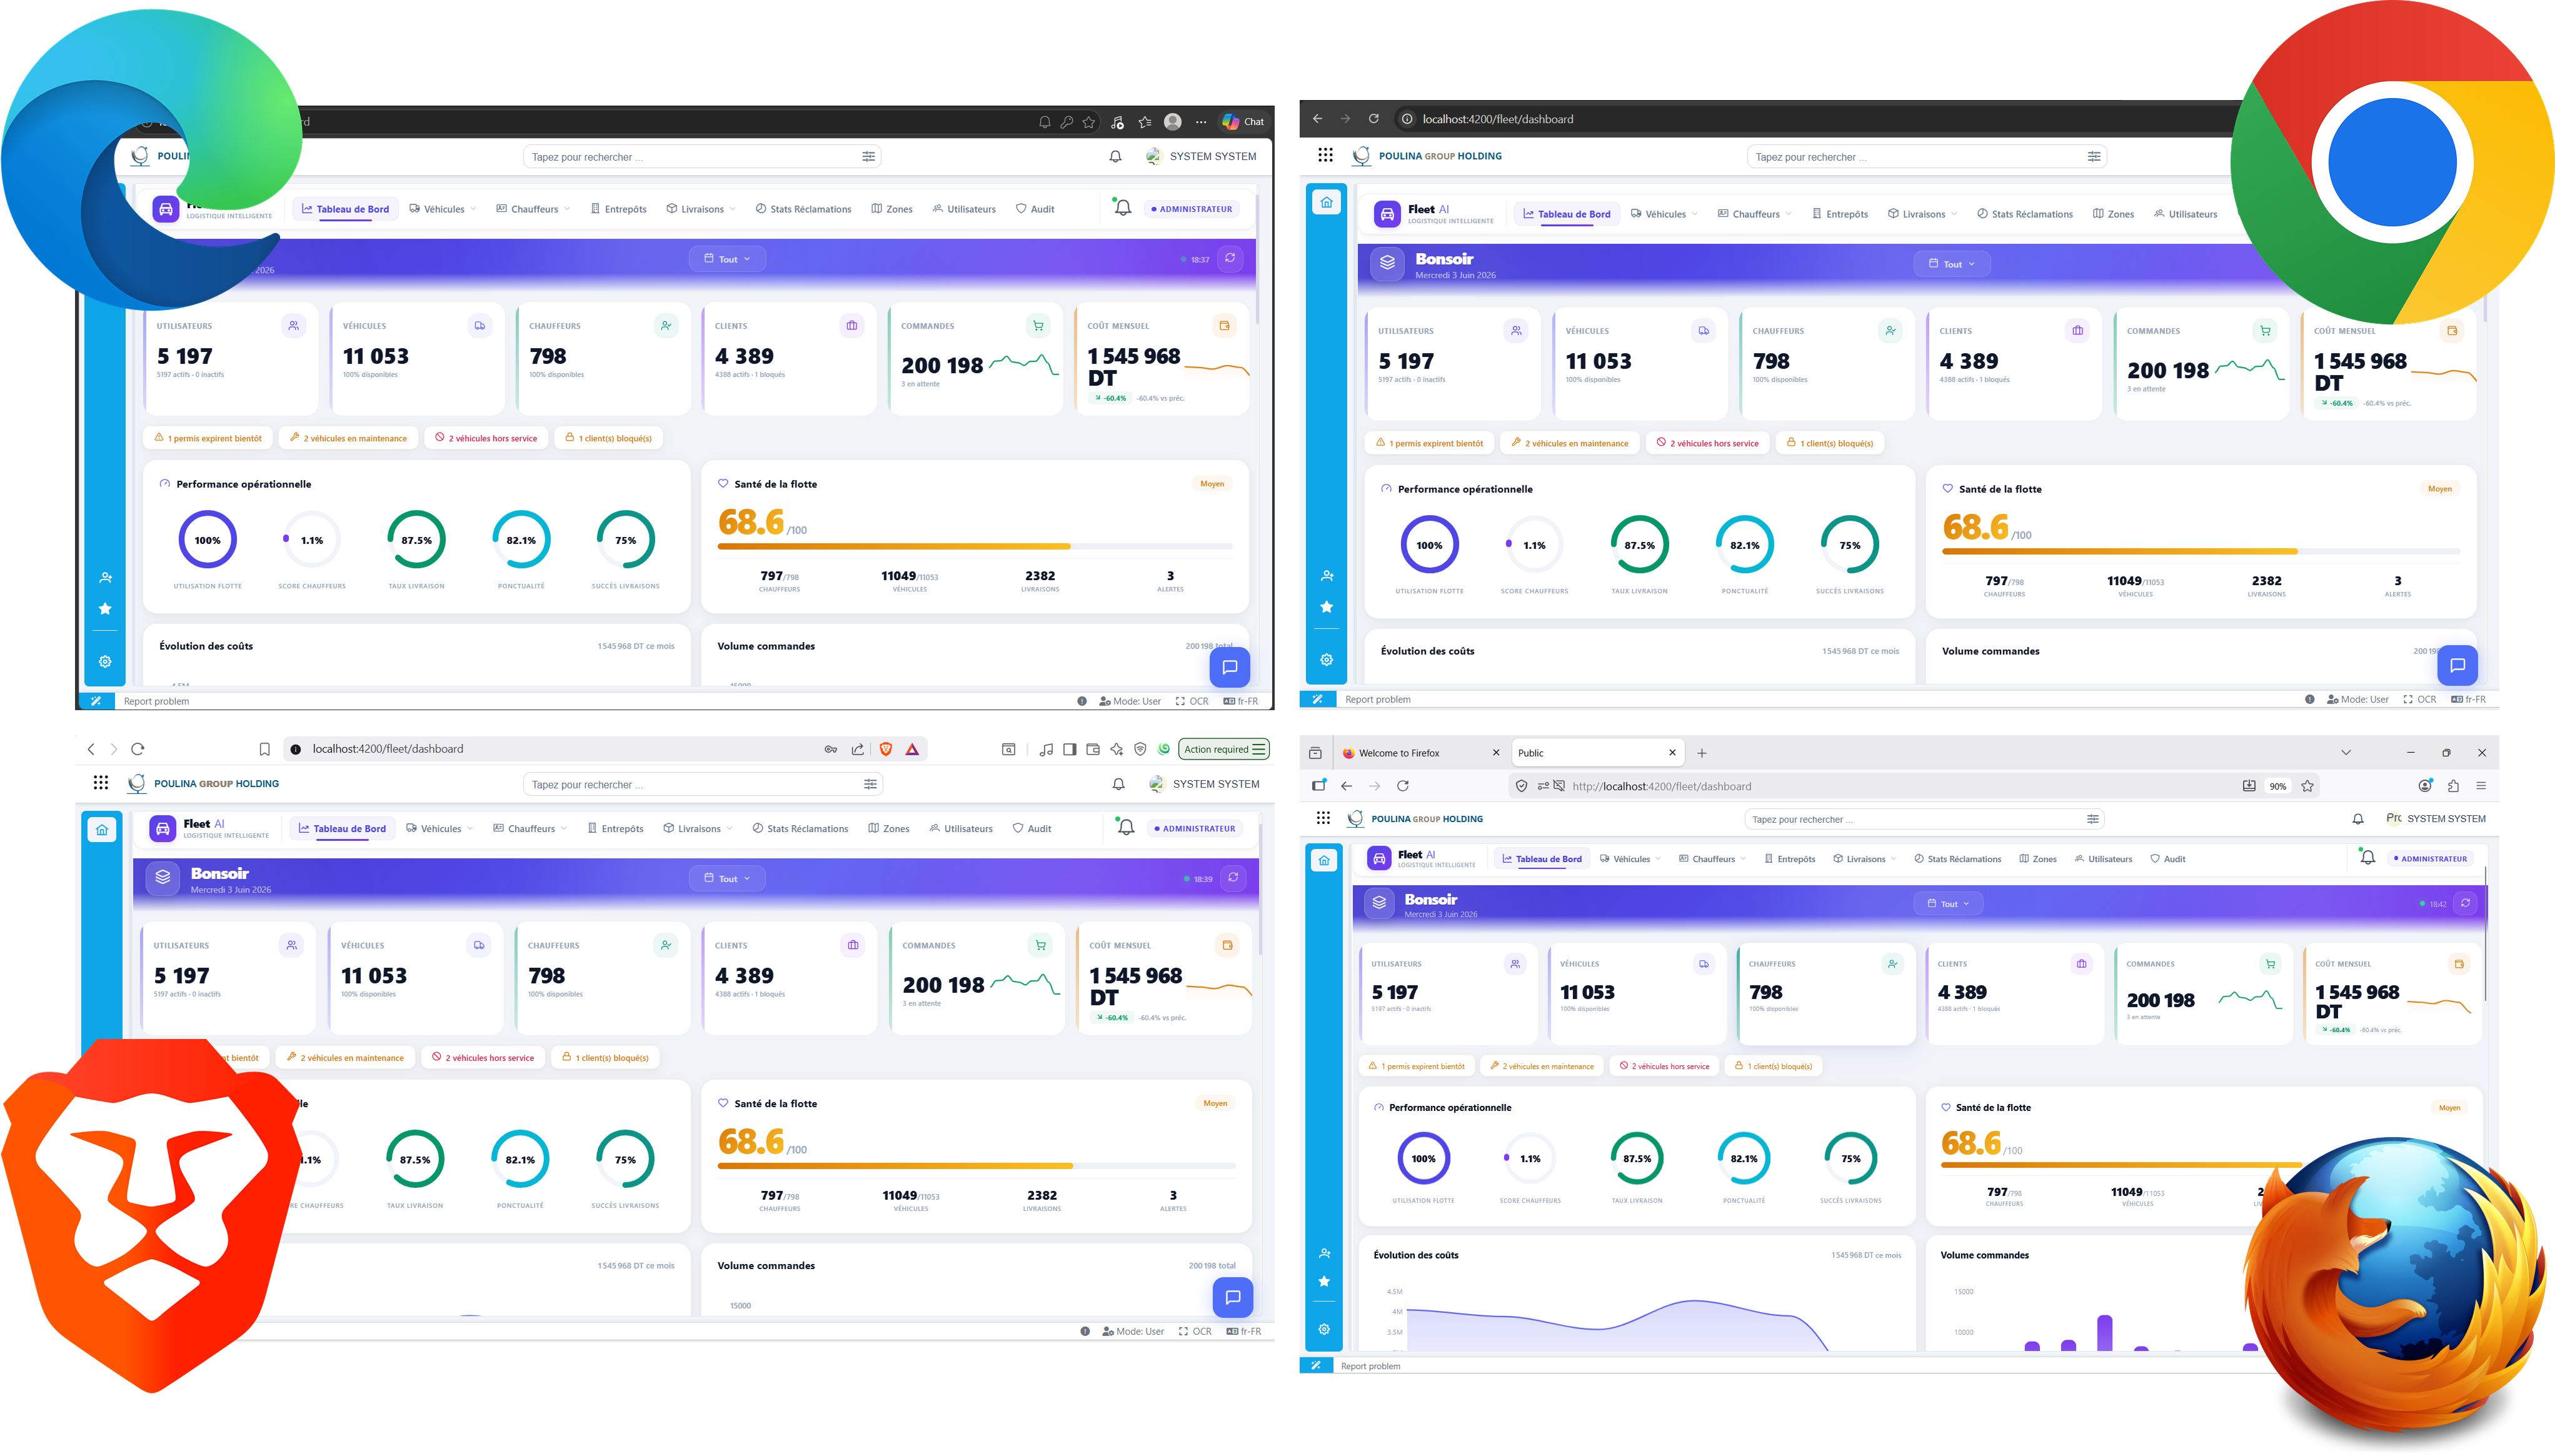
\includegraphics[width=\linewidth, keepaspectratio]{img/capture/web/sp4_test_browser}%
}{%
  \fbox{\parbox{0.9\linewidth}{\centering\vspace{4cm}\textit{[img/capture/web/sp4\_test\_browser.png]}\vspace{4cm}}}%
}
\caption{Exécution d'un test de navigateur sur la page de suivi GPS}
\label{fig:sp4-test}
\end{figure}

\section*{Conclusion}
\addcontentsline{toc}{section}{Conclusion}

Le Sprint~4 couvre l'intégralité de la phase d'exécution terrain de Fleet~AI : suivi GPS temps réel via WebSocket, gestion des trois modes de paiement, traitement des incidents et réclamations avec escalade automatique, et pilotage via tableaux de bord KPI journaliers. Les fonctionnalités de démarrage de sortie avec checklist véhicule, de confirmation terrain (prise de photo, capture chèque, signalement d'arrivée) et de support client sont illustrées par les captures de l'application mobile Flutter. Le Sprint~5 introduira la couche prédictive IA et l'assistant conversationnel.


% ---- Chapitre 8 : Sprint 5 ----
\chapter{Sprint 5 : Prédictions IA \& Chatbot Conversationnel}

\section*{Introduction}
\addcontentsline{toc}{section}{Introduction}
Le Sprint~5 complète Fleet~AI avec la couche d'Intelligence Artificielle. Six modèles de Machine Learning sont entraînés, évalués et déployés via une API FastAPI dédiée : scoring des chauffeurs, prévision de la demande par zone, détection des retards, dimensionnement de flotte, optimisation des tournées et évaluation du risque paiement. Chaque modèle suit la méthodologie CRISP-DM et est intégré directement dans l'interface métier concernée. En complément, un assistant conversationnel Text-to-SQL basé sur un LLM local (Gemma 4 31B via Ollama) permet aux managers d'interroger la base de données analytique en langage naturel, sans écrire de requêtes SQL. Ce sprint transforme Fleet~AI d'un outil de gestion en une plateforme décisionnelle intelligente.

\clearpage

% =============================================================
\section{Sprint Backlog}
% =============================================================

\textbf{Objectif du sprint :} L'objectif est de déployer la couche IA de Fleet~AI : six modèles prédictifs couvrant le scoring chauffeur, la demande, les retards, la flotte, les tournées et le risque paiement, ainsi qu'un assistant conversationnel Text-to-SQL accessible en langage naturel.

\definecolor{headerbg}{HTML}{d5f5e3}
\setlength{\arrayrulewidth}{1pt}

Les story points (SP) reflètent la complexité et l'effort de chaque tâche, estimés selon la suite de Fibonacci.

\begin{longtable}{|>{\raggedright\arraybackslash}p{4.2cm}|>{\raggedright\arraybackslash}p{4.8cm}|>{\raggedright\arraybackslash}p{4.5cm}|c|}
\hline
\rowcolor{headerbg}
\textbf{User Story} & \textbf{Tâche} & \textbf{Critères d'acceptation} & \textbf{\rotatebox{90}{SP}} \\
\hline
\endfirsthead
\hline
\rowcolor{headerbg}
\textbf{User Story} & \textbf{Tâche} & \textbf{Critères d'acceptation} & \textbf{\rotatebox{90}{SP}} \\
\hline
\endhead
\hline
\endfoot

%------ US-078 ------
\multirow{2}{=}{En tant que Planificateur, je veux des prédictions de la demande par zone et par jour dans mon tableau de bord afin d'anticiper les besoins en flotte.}
& Entraîner un modèle de prédiction de la demande à partir des données historiques de livraisons et le déployer dans le système. & Le modèle prédit la demande 7 jours à l'avance avec une précision jugée acceptable par l'équipe. & 8 \\
\cline{2-4}
& Afficher les prédictions de demande par zone et par jour dans le tableau de bord du Planificateur sous forme de graphique. & Les prédictions par zone et par jour sont affichées sous forme de graphique consultable. & 5 \\
\hline

%------ US-079 ------
\multirow{2}{=}{En tant que Planificateur, je veux des prédictions de retard pour chaque tournée dans mon tableau de bord afin d'agir préventivement.}
& Développer un modèle d'identification des tournées à risque de retard à partir des données historiques et des conditions opérationnelles. & Le modèle identifie les tournées à risque avec un taux de détection acceptable. & 5 \\
\cline{2-4}
& Afficher les tournées à risque avec un indicateur de confiance dans le tableau de bord du Planificateur. & Les tournées à risque sont mises en évidence avec un indicateur de niveau de risque (faible/moyen/élevé). & 3 \\
\hline

%------ US-080 ------
\multirow{2}{=}{En tant que Manager, je veux voir le niveau de confiance des prédictions dans mon tableau de bord afin de calibrer ma prise de décision.}
& Intégrer un indicateur de confiance à chaque prédiction exposée dans le tableau de bord Manager. & Chaque prédiction expose un niveau de confiance visible dans le tableau de bord. & 2 \\
\cline{2-4}
& Afficher l'indicateur de confiance par un repère visuel coloré sur chaque prédiction. & L'indicateur est visible sur chaque prédiction dans le tableau de bord. & 1 \\
\hline

%------ US-081 ------
\multirow{2}{=}{En tant qu'Administrateur, je veux que les modèles de prédiction soient réentraînés automatiquement périodiquement afin de maintenir leur précision.}
& Configurer un réentraînement automatique périodique des modèles de prédiction selon un calendrier défini. & Le réentraînement se déclenche automatiquement selon le calendrier configuré. & 3 \\
\cline{2-4}
& Alerter automatiquement le Manager si les indicateurs de performance des modèles se dégradent après réentraînement. & Une alerte est envoyée au Manager si la précision du modèle descend sous le seuil acceptable. & 2 \\
\hline

%------ US-082 ------
\multirow{2}{=}{En tant que Manager, je veux comparer les prédictions avec les réalisations dans mon tableau de bord afin d'évaluer la fiabilité du modèle.}
& Calculer et exposer au Manager l'écart entre les prédictions et les réalisations par zone et par semaine. & Le tableau comparatif affiche l'écart moyen par semaine et par zone. & 3 \\
\cline{2-4}
& Afficher la comparaison prédictions/réalisations avec filtres par période et par zone dans le tableau de bord. & Le graphique comparatif s'affiche avec filtres par période et par zone. & 2 \\
\hline

%------ US-083 ------
\multirow{2}{=}{En tant que Planificateur, je veux des recommandations pour le dimensionnement de la flotte dans mon tableau de bord afin d'optimiser le nombre de véhicules par zone.}
& Générer des recommandations de dimensionnement de flotte basées sur la demande prédite par zone. & Le système suggère le nombre optimal de véhicules par zone selon la demande prédite. & 3 \\
\cline{2-4}
& Afficher les recommandations de dimensionnement dans le tableau de bord avec comparaison face à la flotte actuelle. & Les recommandations sont affichées avec comparaison par rapport à la flotte existante. & 2 \\
\hline


%------ US-144 ------
\multirow{2}{=}{En tant que Manager, je veux interroger la base de données en langage naturel via un chatbot afin d'obtenir des analyses personnalisées.}
& Intégrer un modèle LLM local (Gemma) avec un pipeline Text-to-SQL pour traduire les questions en requêtes de base de données. & Le modèle génère des requêtes SQL valides correspondant aux intentions des utilisateurs. & 3 \\
\cline{2-4}
& Afficher l'interface de conversation dans l'application web avec historique des questions-réponses. & L'interface de chat est fonctionnelle ; l'historique est sauvegardé. & 2 \\
\hline

%------ US-145 ------
\multirow{2}{=}{En tant qu'Administrateur, je veux que le chatbot sécurise l'accès aux données selon le rôle de l'utilisateur afin de garantir la confidentialité.}
& Implémenter un validateur SQL (SQL Validator) pour bloquer les opérations d'écriture et vérifier les accès aux tables. & Le chatbot refuse toute requête DML ou DDL ; seules les tables autorisées sont interrogées. & 2 \\
\cline{2-4}
& Appliquer la sécurité au niveau des lignes (RLS) pour limiter les résultats au périmètre de l'utilisateur courant. & Les résultats sont filtrés selon le rôle (ex: le Manager ne voit que les stats de son périmètre). & 1 \\
\hline

\caption{Sprint Backlog du Sprint 5 --- Prédictions IA \& Chatbot Conversationnel}
\end{longtable}
\setlength{\arrayrulewidth}{0.4pt}


% =============================================================
\section{Modélisation IA selon la méthodologie CRISP-DM}
% =============================================================

Le sprint~5 introduit la couche prédictive de Fleet~AI : six modèles ML déployés via FastAPI, un chatbot Text-to-SQL sur LLM local, et un pipeline ETL industrialisé. La méthodologie \textbf{CRISP-DM} (\textit{Cross-Industry Standard Process for Data Mining}) cadre l'ensemble du cycle de vie, de la compréhension métier au déploiement en production.

% -----------------------------------------------------------
\subsection{Pipeline ETL -- Extraction, Transformation, Load}
% -----------------------------------------------------------

Avant tout entraînement, les données brutes issues du WFMS -- commandes ERP au format JSON, traces GPS, profils chauffeurs, historiques de paiement et logs d'audit -- doivent être préparées. Cette phase s'est révélée la difficulté centrale du sprint : la qualité des prédictions dépend directement de la rigueur du pipeline ETL.

% ============================================================
% FIGURE 8.1 — Pipeline ETL Fleet AI
% ============================================================
%
%  Layout (vertical, top-to-bottom) :
%
%   ┌─────────────────────────────────────────────────────────┐
%   │  Sources ERP / WFMS  (Ligne 0 — 5 nœuds gris)          │
%   │  S1   S2   S3   S4   S5                                 │
%   ├─────────────────────────────────────────────────────────┤
%   │  Étape 1 — Pré-traitement (Ligne 1 — 4 nœuds bleus)    │
%   │  E1 → E2 → E3 → E4                                     │
%   ├─────────────────────────────────────────────────────────┤
%   │  Étape 2 — Enrichissement (Ligne 2 — 4 nœuds)          │
%   │  E5 → E6 → E7(vert) → E8(bleu foncé)                   │
%   └─────────────────────────────────────────────────────────┘
%
%  Règles de routage sans croisement :
%  • S1→E1 : vertical direct
%  • S2,S3 → E2 : descendent à y=-1.4cm puis convergent vers E2
%  • S4,S5 → E4 : descendent à y=-1.4cm puis convergent vers E4
%  • E1→E5 : vertical direct (côté gauche)
%  • E4→E5 : passe en-dessous de la ligne 1 via y=-5.0cm
%             puis remonte à gauche (couloir x=-1.0cm) → E5
%  • E1→E2→E3→E4 : horizontaux directs
%  • E5→E6→E7→E8 : horizontaux directs
%
% ============================================================
% FIGURE 8.1 — Pipeline ETL Fleet AI
% ============================================================
\begin{figure}[H]
\centering
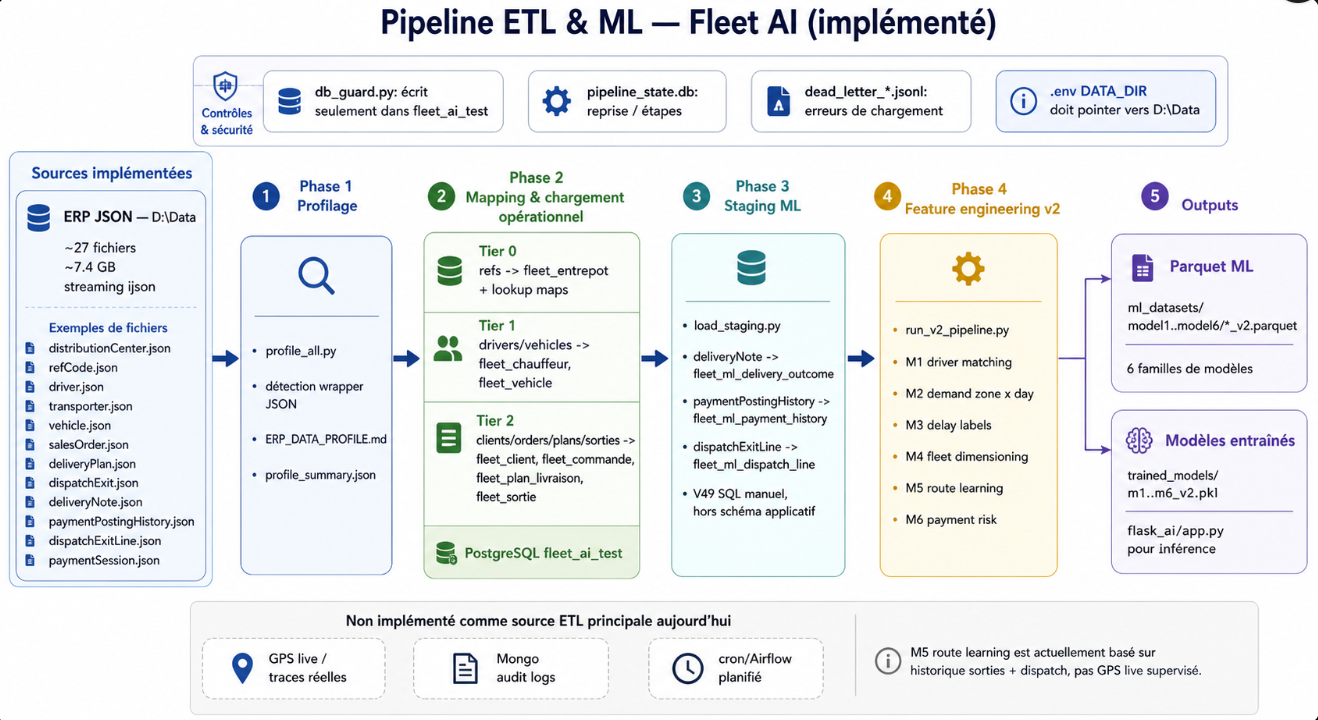
\includegraphics[width=\linewidth, keepaspectratio]{img/figure/ETL}
\caption{Pipeline ETL Fleet~AI --- Vue d'ensemble : de l'extraction ERP/WFMS à la sérialisation Parquet et au chargement PostgreSQL}
\label{fig:etl-pipeline}
\end{figure}



\subsubsection{Sources et extraction}

Le WFMS expose ses données sous forme de fichiers JSON hétérogènes dont la structure varie selon l'entité source (commandes, tournées, paiements, retours). Cinq catégories de sources sont ingérées :

\begin{itemize}
  \item fichiers de commandes ERP (champs manquants fréquents, encodages mixtes) ;
  \item traces GPS horodatées (intervalles irréguliers, coordonnées aberrantes) ;
  \item historiques de livraisons et statuts ;
  \item données client et transactions de paiement ;
  \item logs d'audit et événements métier.
\end{itemize}

\subsubsection{Transformation et nettoyage}

Le pipeline applique les transformations suivantes dans cet ordre :

\begin{enumerate}
  \item \textbf{Nettoyage} : suppression des doublons, correction des coordonnées GPS hors périmètre, normalisation des dates (ISO-8601).
  \item \textbf{Imputation} : valeurs manquantes imputées par médiane (variables continues) ou mode (variables catégorielles). Les colonnes dépassant 40\,\% de valeurs nulles sont exclues.
  \item \textbf{Résolution des incohérences} : détection par règles métier (ex. : livraison \texttt{LIVRÉE} sans horodatage, montant négatif) et mise en \textit{dead-letter queue} pour révision manuelle.
  \item \textbf{Normalisation} : variables numériques standardisées (StandardScaler) ; variables catégorielles encodées (One-Hot pour les zones géographiques, ordinal pour les niveaux de risque).
  \item \textbf{Feature engineering} : construction de variables métier dérivées -- taux de réussite historique par chauffeur, délai moyen de livraison par zone, charge hebdomadaire, score de ponctualité glissant sur 30~jours.
  \item \textbf{Agrégation temporelle} : fenêtres glissantes (1h, 24h, 7~jours) pour capturer les tendances de saisonnalité et les pics de demande.
\end{enumerate}

\subsubsection{Sérialisation et chargement}

Chaque modèle dispose d'un dataset dédié sérialisé au format \textbf{Parquet} (compression Snappy), choisi pour ses performances en lecture colonnaire et sa compatibilité native avec Pandas et PyArrow.

\begin{table}[H]
\centering
\setlength{\arrayrulewidth}{1pt}
\begin{tabular}{|l|l|r|}
\hline
\rowcolor{headerbg}
\textbf{Modèle} & \textbf{Dataset Parquet} & \textbf{Taille} \\
\hline
M1 -- Driver Scoring & \texttt{driver\_order\_pairs\_v2.parquet} & 11,5~Mo \\
\hline
M2 -- Demand Forecast & \texttt{demand\_features\_v2.parquet} & 2,3~Mo \\
\hline
M3 -- Delay Prediction & \texttt{delay\_features\_v2.parquet} & 8,9~Mo \\
\hline
M4 -- Fleet Dimensioning & \texttt{fleet\_features\_v2.parquet} & 1,6~Mo \\
\hline
M5 -- Route Learning & \texttt{route\_features\_v2.parquet} & 10,0~Mo \\
\hline
M6 -- Payment Risk & \texttt{payment\_risk\_v2.parquet} & 0,3~Mo \\
\hline
\end{tabular}
\caption{Datasets Parquet générés par le pipeline ETL}
\label{tab:datasets-parquet}
\end{table}
\setlength{\arrayrulewidth}{0.4pt}




% -----------------------------------------------------------
\subsection{M1 -- Driver Scoring : démarche CRISP-DM détaillée}
% -----------------------------------------------------------

Le modèle M1 constitue la référence pédagogique du sprint. Chaque phase CRISP-DM est détaillée ci-après.

\begin{figure}[H]
\centering
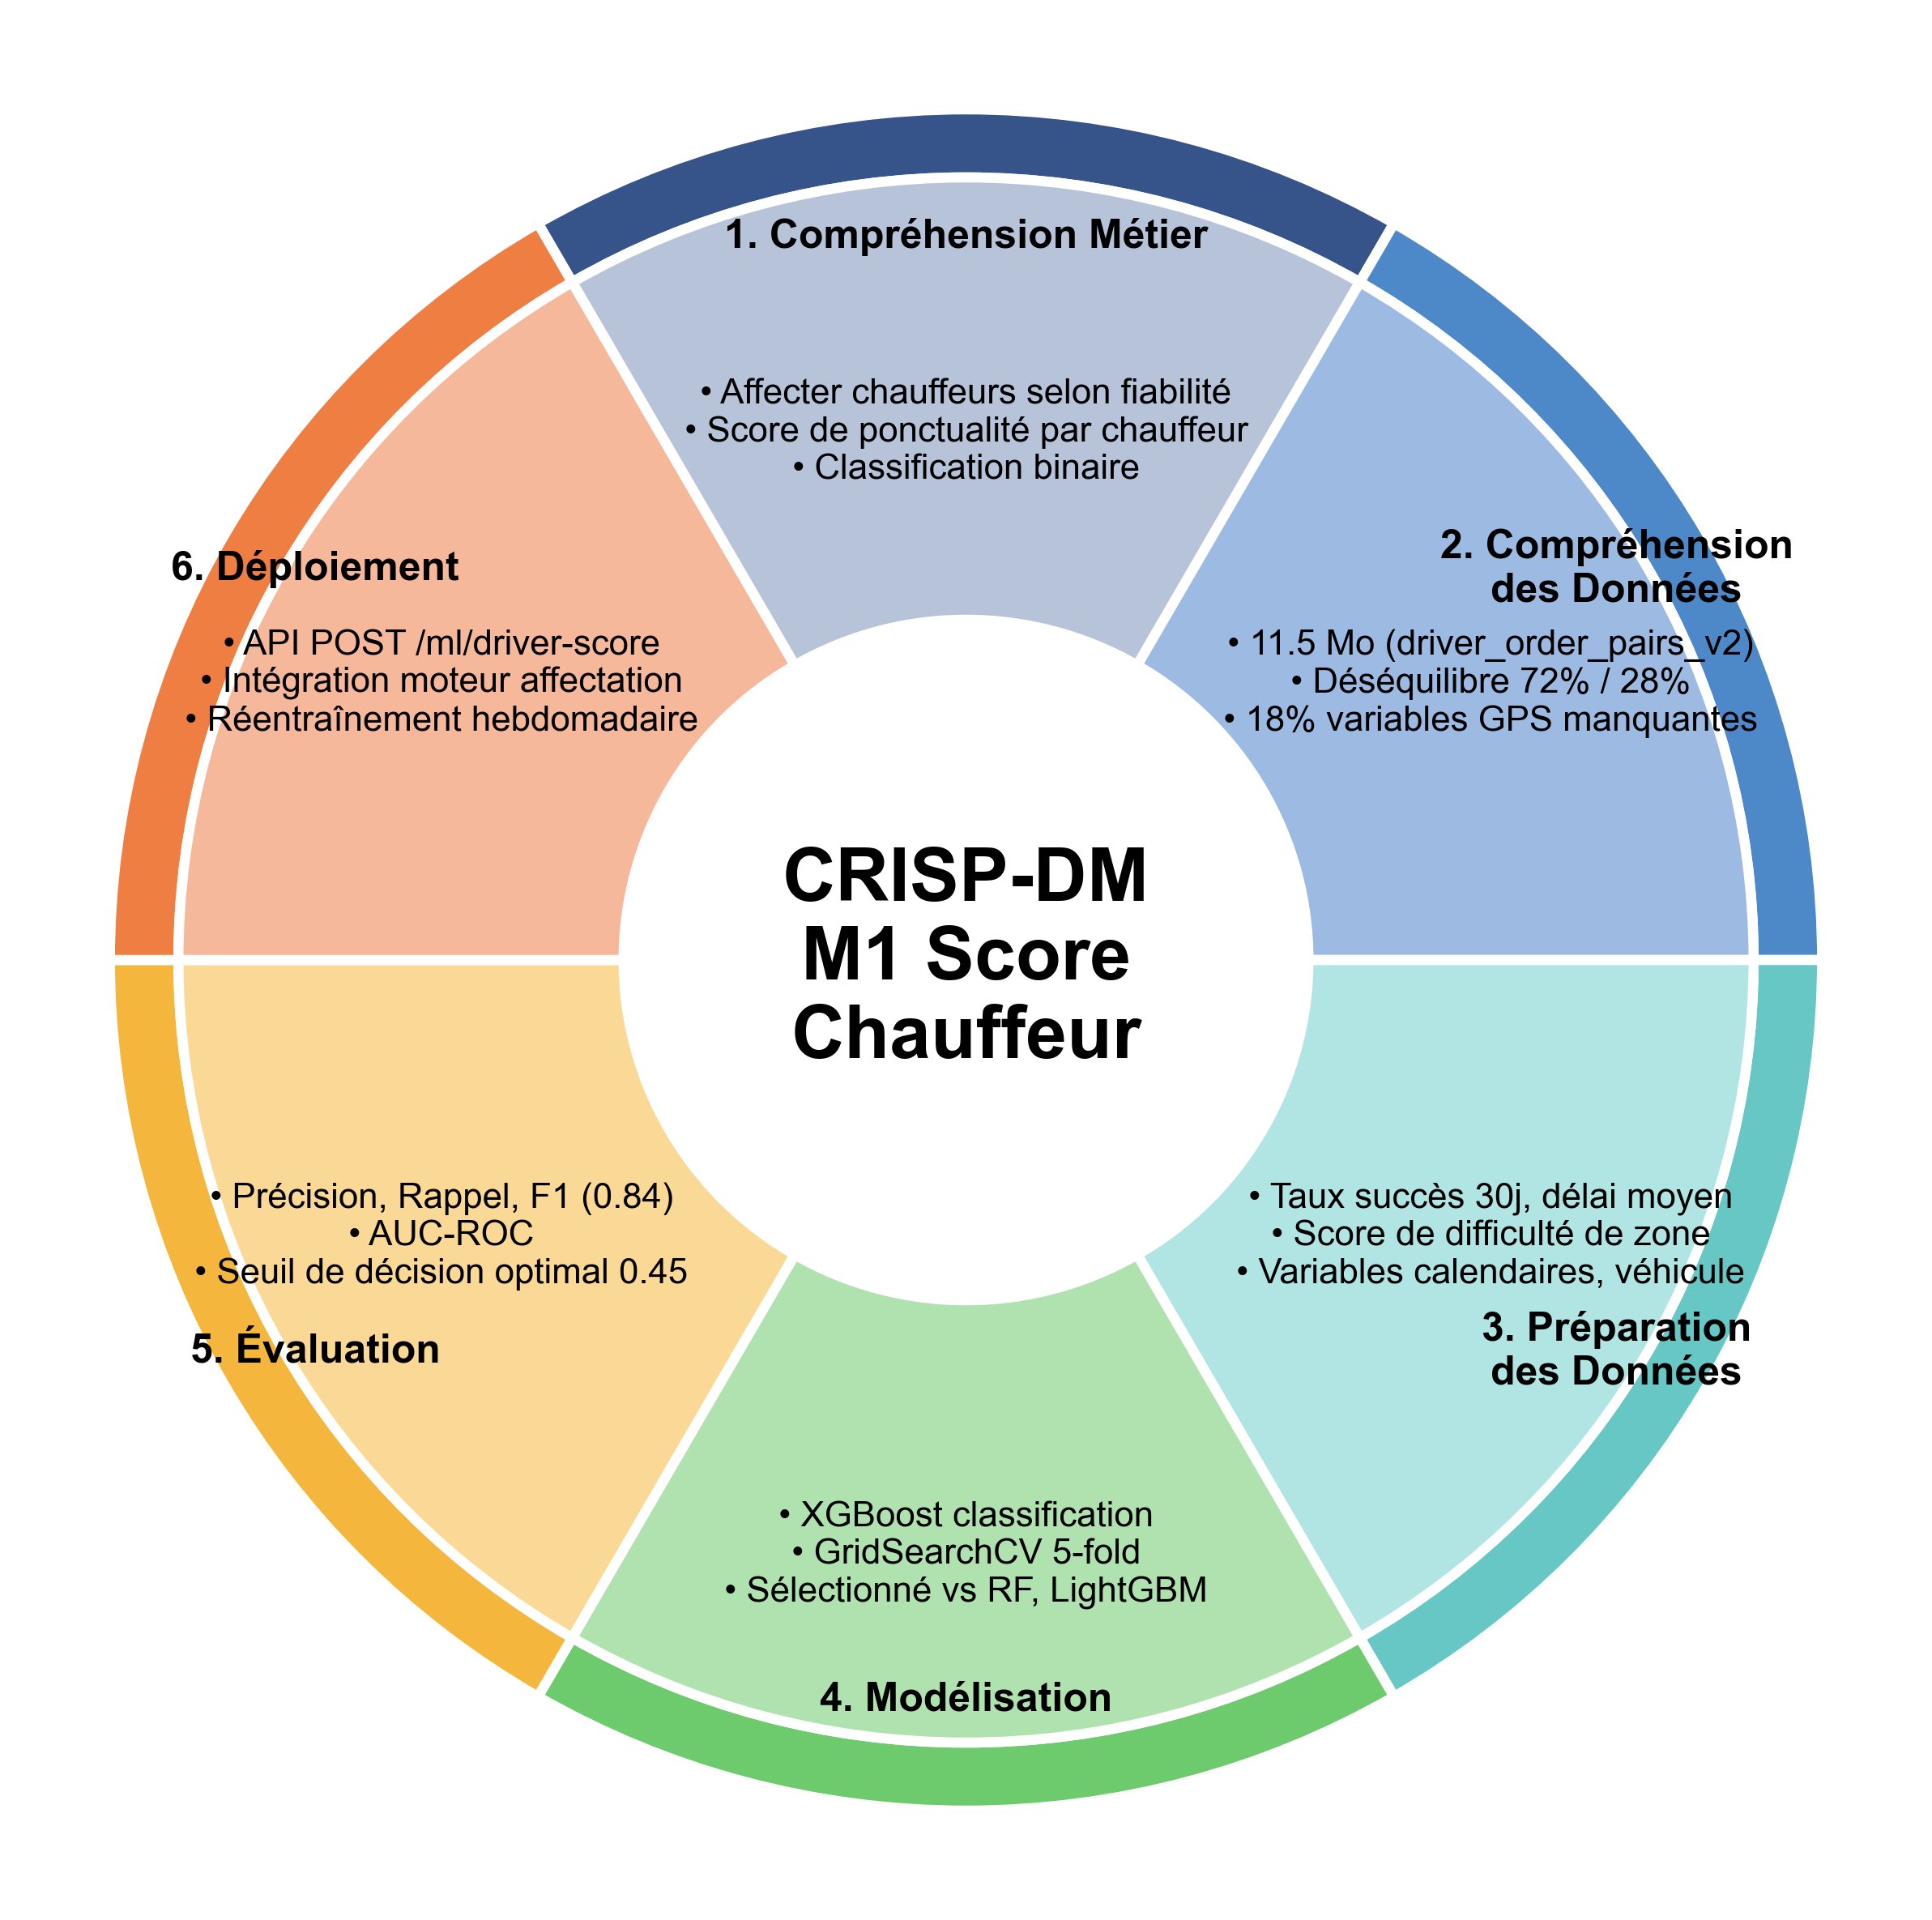
\includegraphics[width=0.90\linewidth]{img/crisp/crisp_dm_m1_driver}
\caption{Diagramme CRISP-DM -- M1 Score Chauffeur}
\label{fig:crisp-m1}
\end{figure}

\paragraph{Compréhension métier.}
Le planificateur de PGH doit affecter les chauffeurs aux tournées les plus adaptées à leur fiabilité. L'objectif est de produire un score de fiabilité par chauffeur, fondé sur son historique de ponctualité, afin d'alimenter le moteur d'affectation de Fleet~AI.

Problème modélisé : classification binaire de la ponctualité (\texttt{was\_on\_time} $\in \{0, 1\}$).

\paragraph{Compréhension des données.}
Dataset principal : \texttt{driver\_order\_pairs\_v2.parquet} (11,5~Mo, paires chauffeur--commande enrichies). Features initiales explorées : profil du chauffeur (ancienneté, type de permis), zone de livraison, tranche horaire, conditions de la tournée, historique de 90~jours.

Principaux constats d'exploration :
\begin{itemize}
  \item distribution déséquilibrée (72\,\% on-time / 28\,\% retard) ;
  \item forte corrélation entre zone et taux de retard ;
  \item variables GPS manquantes à 18\,\% -- gérées nativement par XGBoost.
\end{itemize}

\paragraph{Préparation des données.}
Application du pipeline ETL (\S~8.2.1). Features retenues après sélection :

\begin{itemize}
  \item \texttt{driver\_success\_rate\_30d} -- taux de réussite glissant 30~jours ;
  \item \texttt{avg\_delivery\_delay\_min} -- délai moyen historique en minutes ;
  \item \texttt{zone\_difficulty\_score} -- score de complexité de la zone ;
  \item \texttt{order\_count\_day} -- charge journalière du chauffeur ;
  \item \texttt{hour\_of\_day}, \texttt{day\_of\_week} -- variables calendaires ;
  \item \texttt{vehicle\_type\_encoded} -- type de véhicule (One-Hot).
\end{itemize}

\paragraph{Modélisation et justification du modèle.}
Cinq algorithmes ont été évalués lors de cette phase : Régression Logistique, Réseau de Neurones (MLP), Random Forest, LightGBM et XGBoost. Les résultats obtenus sur un jeu de test (20\,\% des données) sont présentés dans le tableau~\ref{tab:m1-evaluation}.

\begin{table}[H]
\centering
\setlength{\arrayrulewidth}{1pt}
\begin{tabular}{|l|c|c|p{4cm}|}
\hline
\rowcolor{headerbg}
\textbf{Algorithme} & \textbf{Précision (Accuracy)} & \textbf{F1-Score} & \textbf{Temps d'entraînement} \\
\hline
Régression Logistique & 68,5\,\% & 0,62 & Très rapide (< 10 s) \\
\hline
Réseau de Neurones (MLP) & 74,2\,\% & 0,71 & Lent ($\approx$ 12 min) \\
\hline
Random Forest & 81,4\,\% & 0,78 & Moyen ($\approx$ 3 min) \\
\hline
LightGBM & 83,1\,\% & 0,81 & Très rapide ($\approx$ 15 s) \\
\hline
\textbf{XGBoost} & \textbf{85,7\,\%} & \textbf{0,84} & \textbf{Rapide ($\approx$ 30 s)} \\
\hline
\end{tabular}
\caption{Comparatif des algorithmes évalués pour le modèle M1}
\label{tab:m1-evaluation}
\end{table}
\setlength{\arrayrulewidth}{0.4pt}

L'algorithme \textbf{XGBoost} a été retenu. En plus de fournir les meilleures performances (F1-Score de 0,84), il gère nativement les valeurs manquantes (fréquentes avec les signaux GPS), résiste bien au surapprentissage grâce à sa régularisation (L1/L2), et offre une grande interprétabilité (importance des features) cruciale pour expliquer les scores aux planificateurs.

Un classificateur XGBoost a donc été entraîné avec une recherche sur grille (\textit{GridSearchCV}, 5-fold stratifié) sur les hyperparamètres : \texttt{max\_depth} $\in$ \{4, 6, 8\}, \texttt{learning\_rate} $\in$ \{0.05, 0.1\}, \texttt{n\_estimators} $\in$ \{200, 400\}. Le paramètre \texttt{scale\_pos\_weight} compense le déséquilibre de classes.

\paragraph{Évaluation.}
Métriques retenues : Précision, Rappel, F1-Score et AUC-ROC. La matrice de confusion valide le seuil de décision optimal à 0.45 (maximisation du F1 sur la classe minoritaire).

\paragraph{Déploiement.}
Le modèle sérialisé (\texttt{joblib}) est exposé via une route FastAPI \texttt{POST /api/v1/ml/driver-score}. Le score retourné (0--100) est intégré directement dans l'algorithme d'affectation de Fleet~AI. Un réentraînement automatique est planifié hebdomadairement.

\paragraph{Intégration dans l'application.}
Le score du modèle M1 est visible par le Planificateur dans le formulaire d'affectation~: les trois meilleurs candidats chauffeurs sont classés par score de fiabilité (0--100), avec la décomposition des critères (zone, charge, performance). Ce score alimente également le module de suggestions du Sprint~5.

\begin{figure}[H]
\centering
\IfFileExists{img/capture/ai/sp5_m1_driver_score_composite.png}{%
  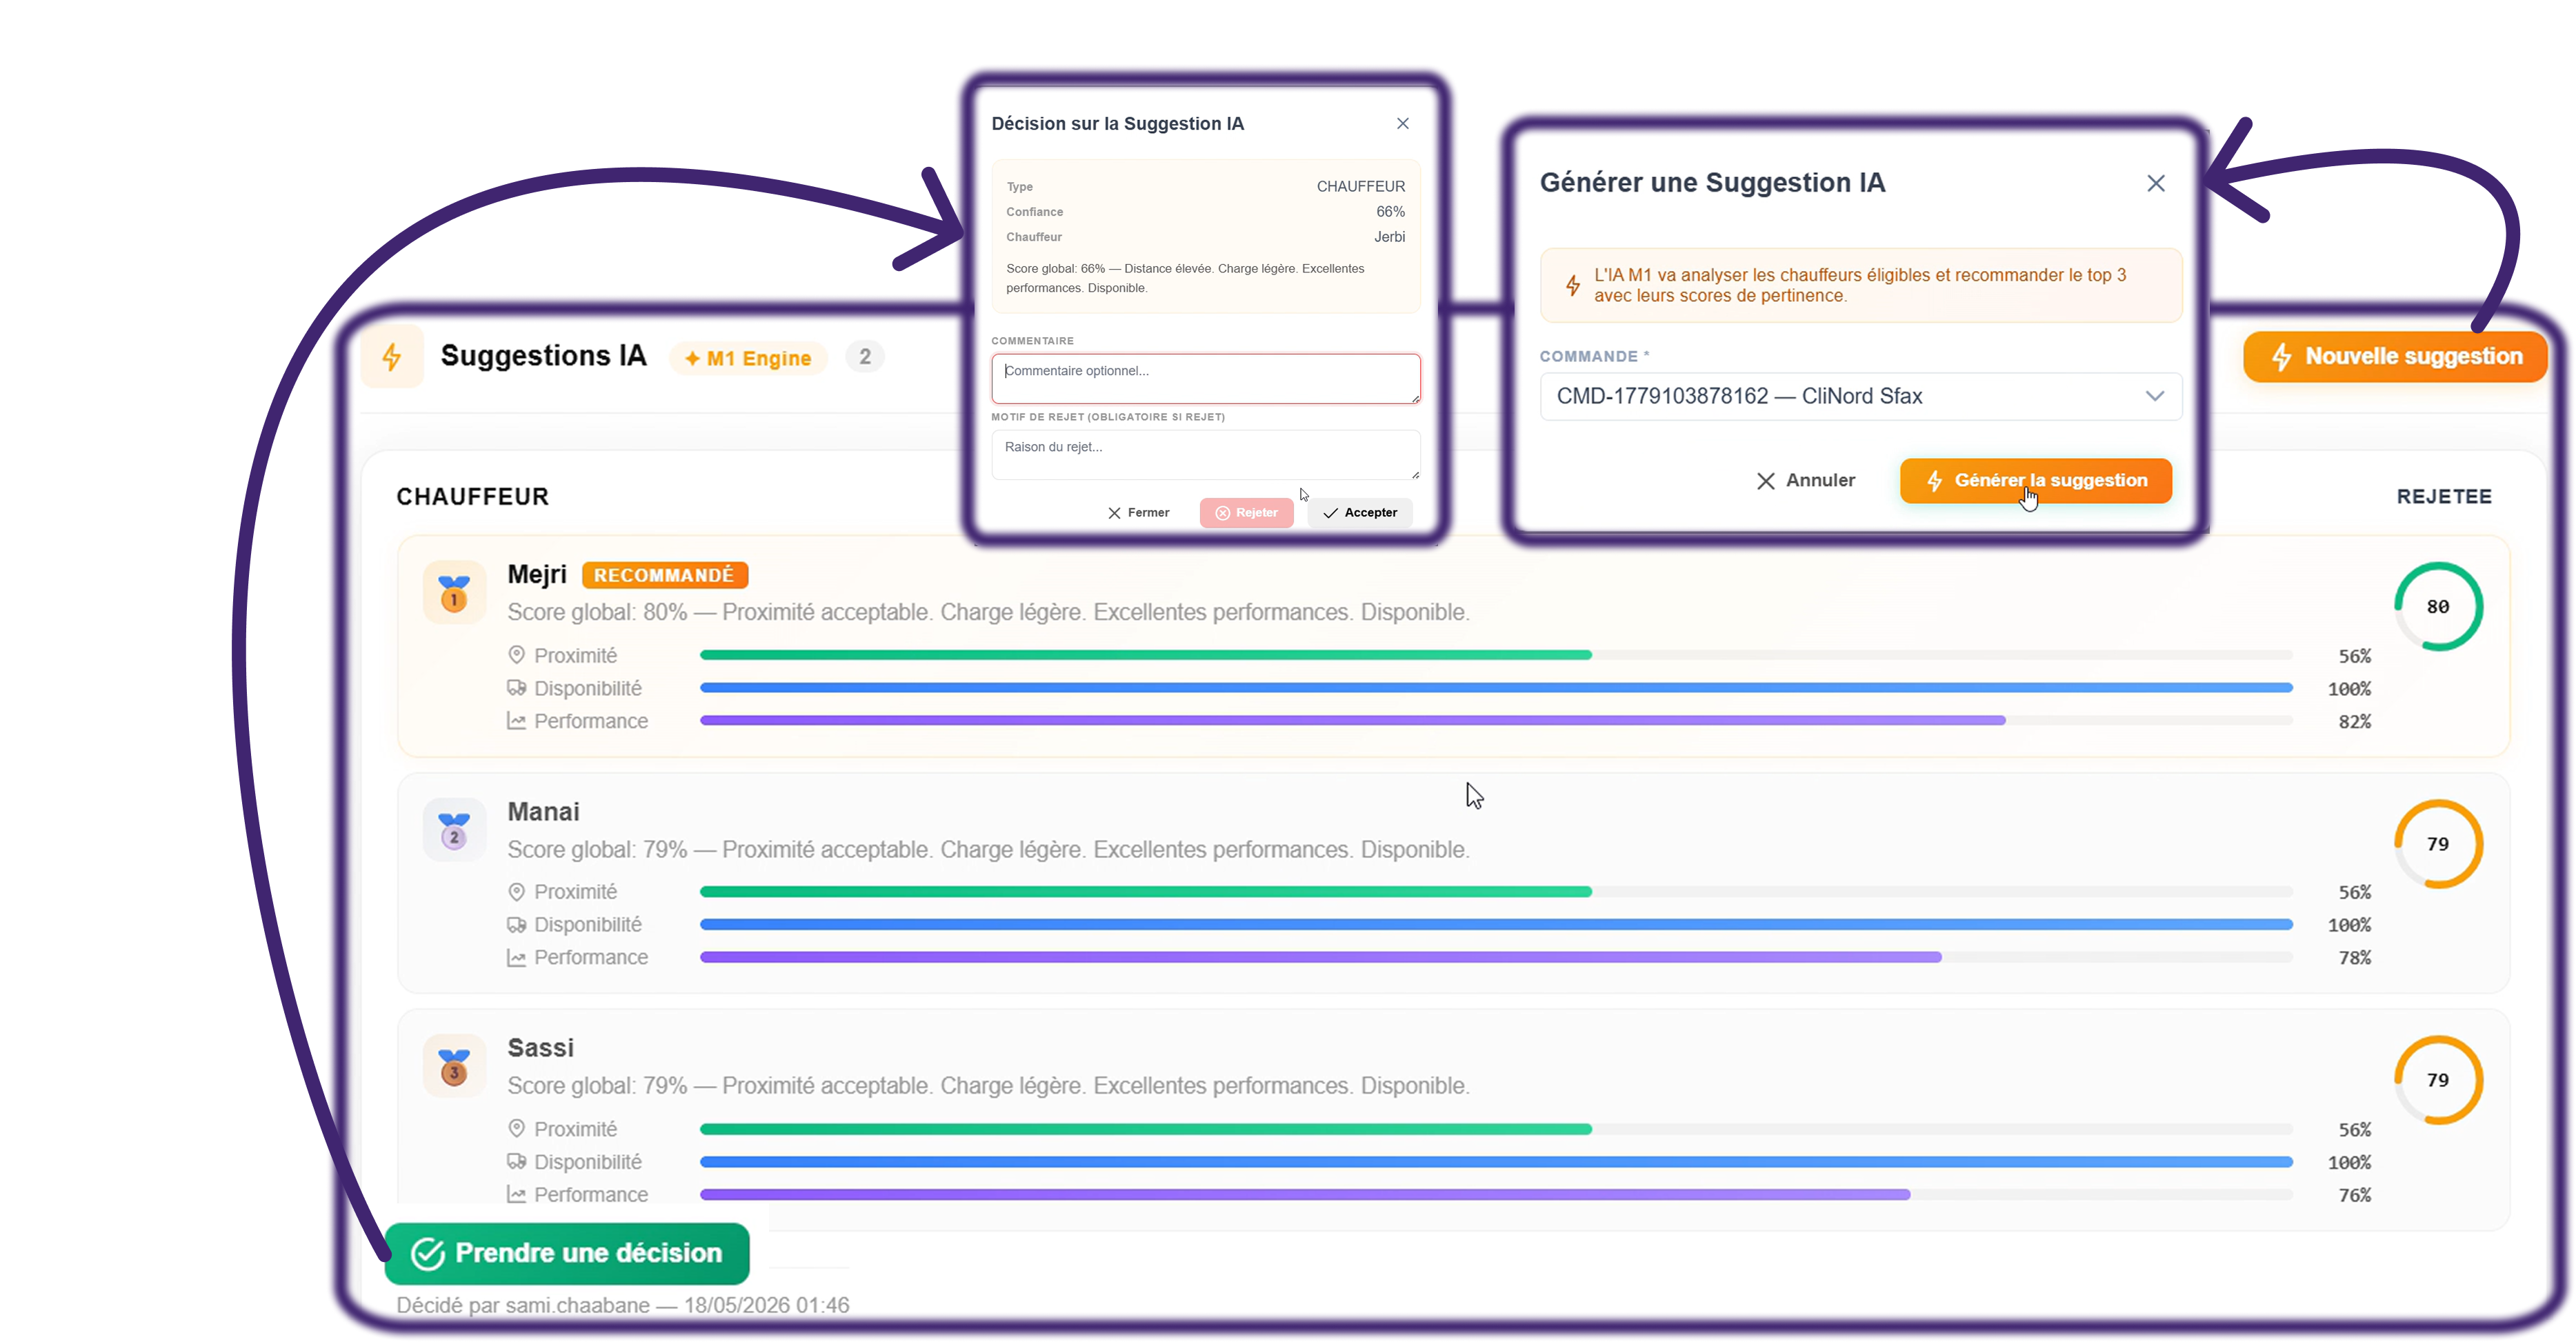
\includegraphics[width=\linewidth, keepaspectratio]{img/capture/ai/sp5_m1_driver_score_composite}%
}{%
  \fbox{\parbox{0.9\linewidth}{\centering\vspace{4cm}\textit{[\`{}img/sp5\_m1\_driver\_score\_composite\`{} --- Capture à réaliser]}\vspace{4cm}}}%
}
\caption{Intégration M1 Driver Scoring : formulaire d'affectation avec scores de fiabilité, top~3 chauffeurs et décomposition des critères}
\label{fig:sp5-m1-integration}
\end{figure}

% -----------------------------------------------------------
\subsection{Modèles prédictifs additionnels (M2 à M6)}
% -----------------------------------------------------------

Les modèles M2 à M6 suivent la même méthodologie CRISP-DM. Pour chacun de ces modèles, l'algorithme XGBoost a été retenu pour les mêmes raisons de performance, de gestion des données tabulaires et de robustesse que celles justifiées lors de la modélisation de M1. Seuls les éléments distinctifs de chaque modèle sont présentés ci-après.

\subsubsection{M2 -- Demand Forecast}

\begin{figure}[H]
\centering
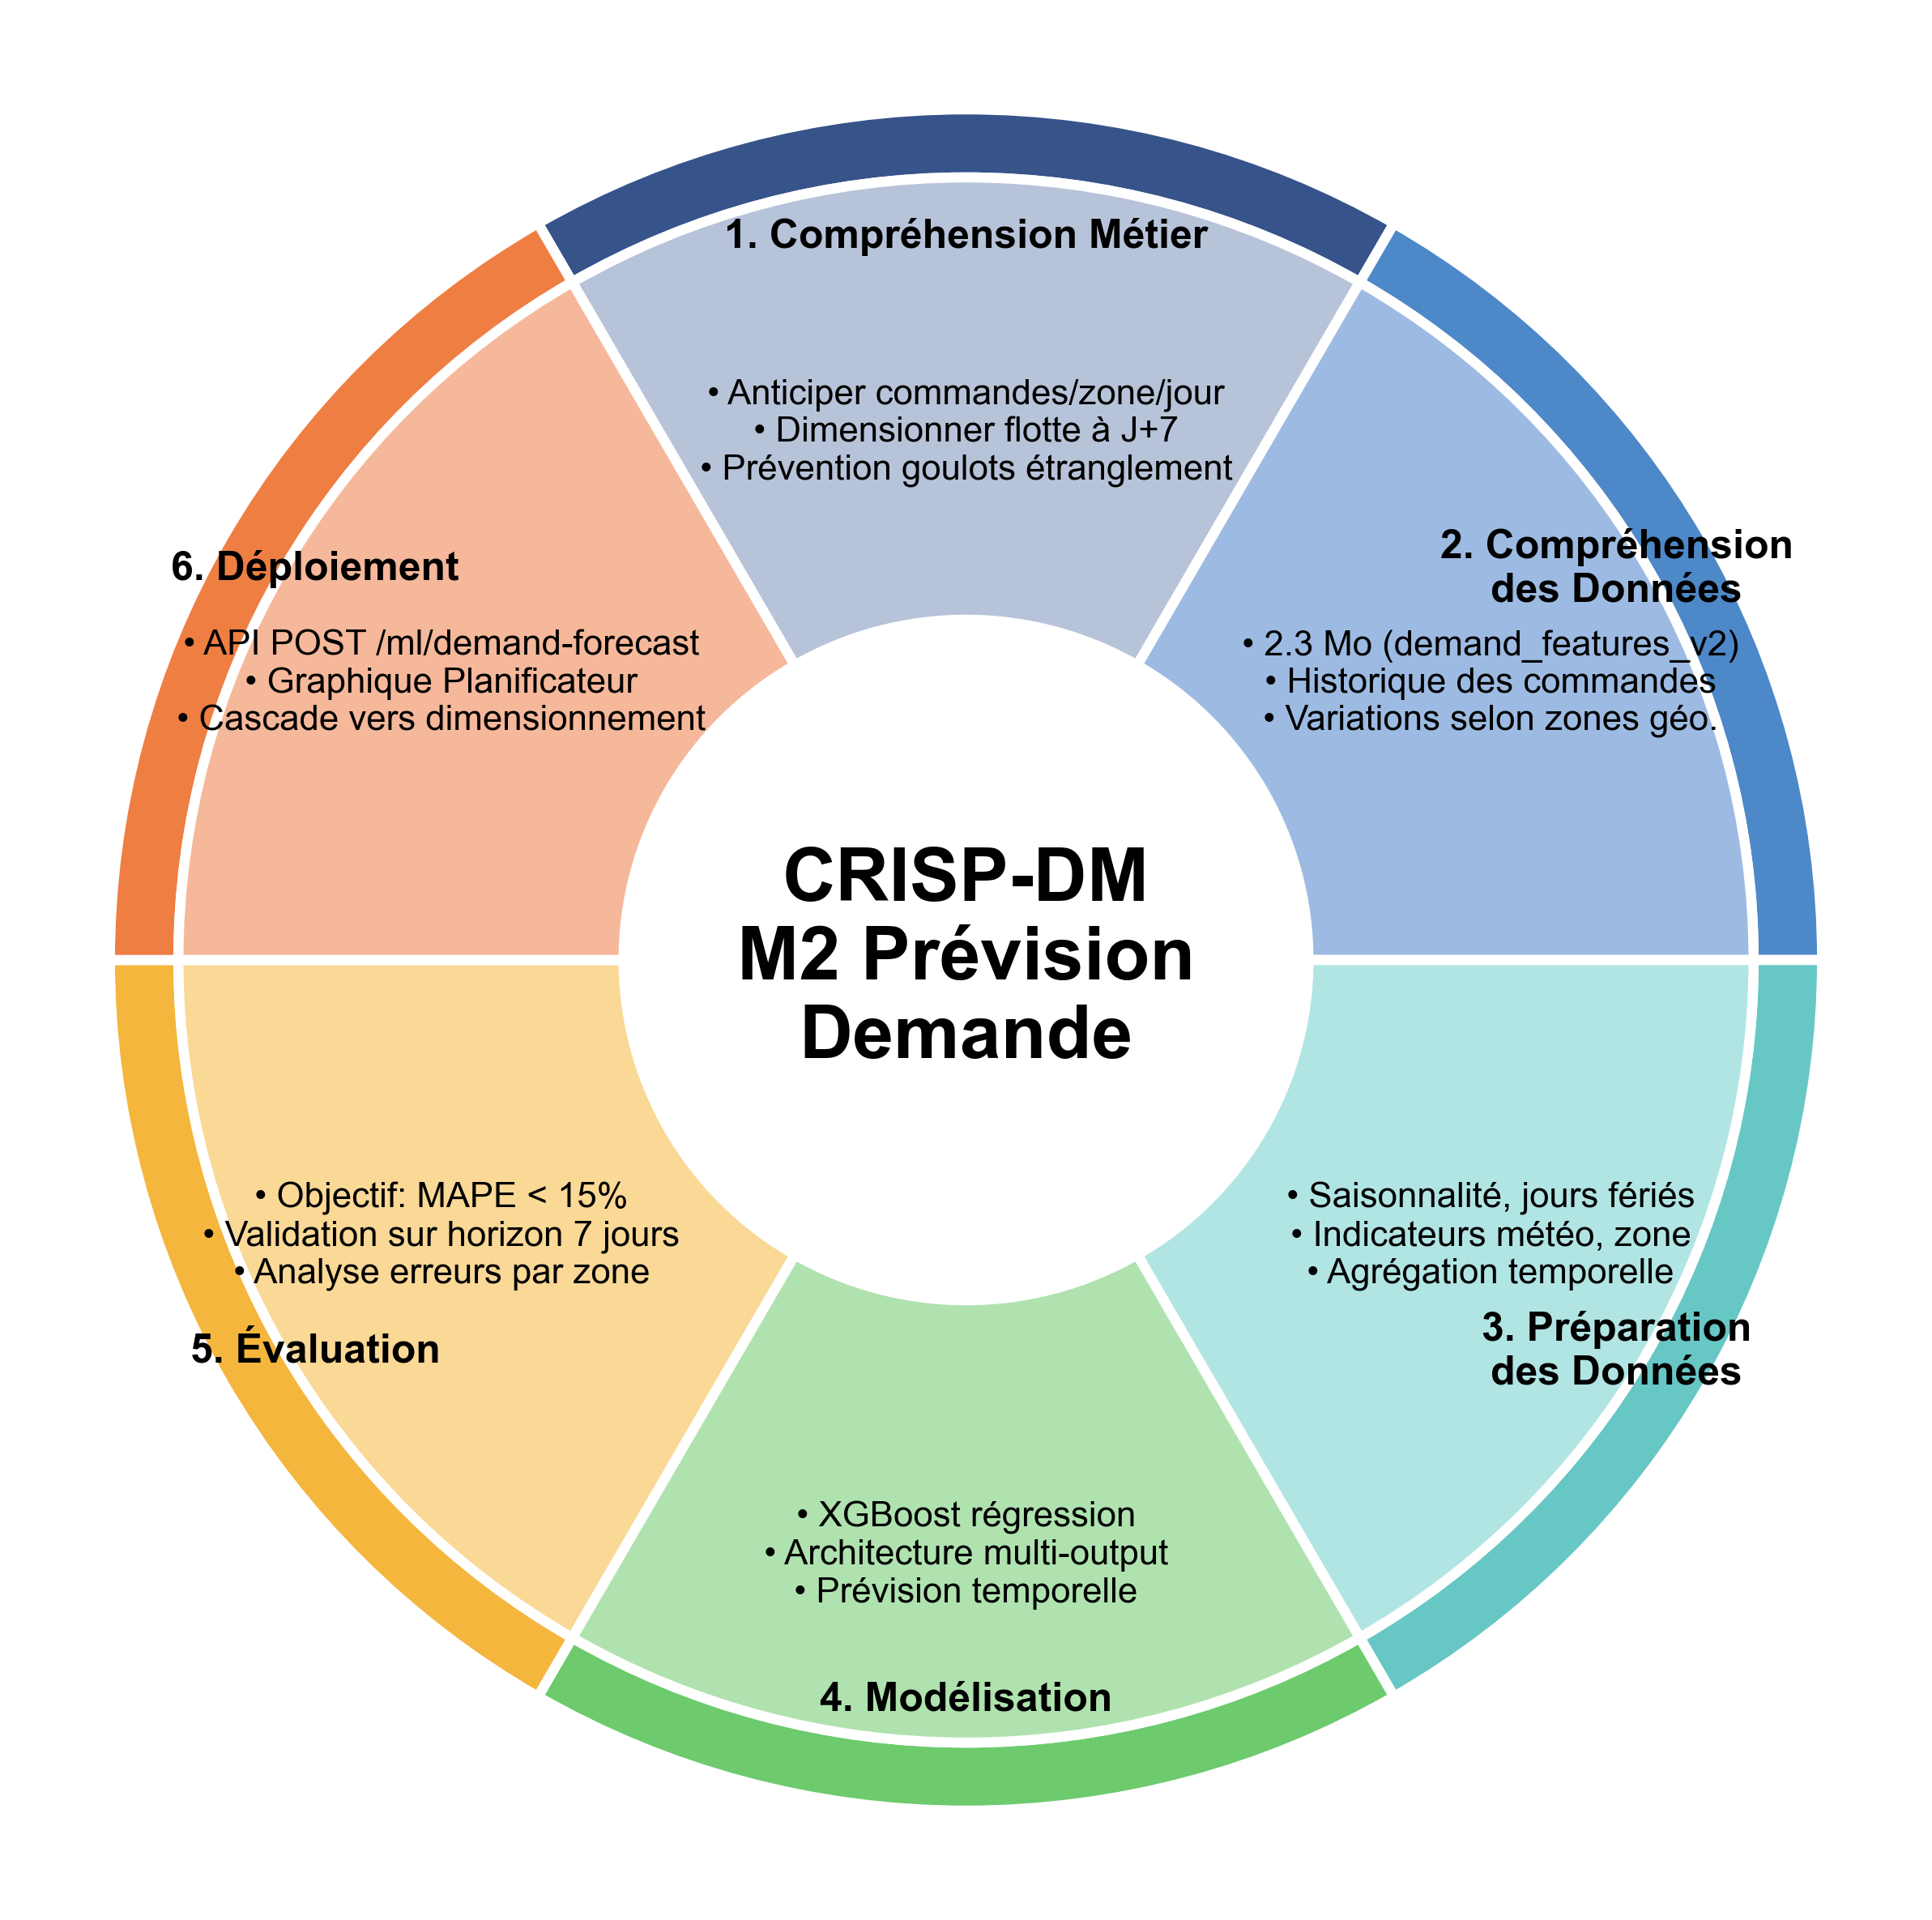
\includegraphics[width=0.88\linewidth]{img/crisp/crisp_dm_m2_demand}
\caption{Diagramme CRISP-DM -- M2 Prévision de la Demande}
\label{fig:crisp-m2}
\end{figure}

\begin{table}[H]
\centering
\setlength{\arrayrulewidth}{1pt}
\begin{tabular}{|p{3.5cm}|p{9.5cm}|}
\hline
\rowcolor{headerbg}
\multicolumn{2}{|c|}{\textbf{M2 -- Demand Forecast}} \\
\hline
\textbf{Objectif métier} & Anticiper le volume de commandes par zone et par jour pour dimensionner la flotte à J+7. \\
\hline
\textbf{Dataset} & \texttt{demand\_features\_v2.parquet} (2,3~Mo) \\
\hline
\textbf{Features clés} & Historique de commandes, saisonnalité, jours fériés, zone géographique, indicateurs météo. \\
\hline
\textbf{Algorithme} & XGBoost régression multi-output (une sortie par zone). \\
\hline
\textbf{Métrique cible} & MAPE $<$ 15\,\% sur l'horizon 7~jours. \\
\hline
\textbf{Intégration} & Tableau de bord Planificateur -- graphique de prévision par zone. \\
\hline
\end{tabular}
\caption{Fiche synthétique -- M2 Demand Forecast}
\label{tab:m2-summary}
\end{table}
\setlength{\arrayrulewidth}{0.4pt}

\paragraph{Intégration dans l'application.}
Les prévisions de la demande par zone et par jour sont affichées sous forme de graphique interactif dans le tableau de bord du Planificateur. L'horizon est de 7~jours avec un indicateur de fiabilité (MAPE).

\begin{figure}[H]
\centering
\IfFileExists{img/capture/ai/sp5_m2_demand_forecast_composite.png}{%
  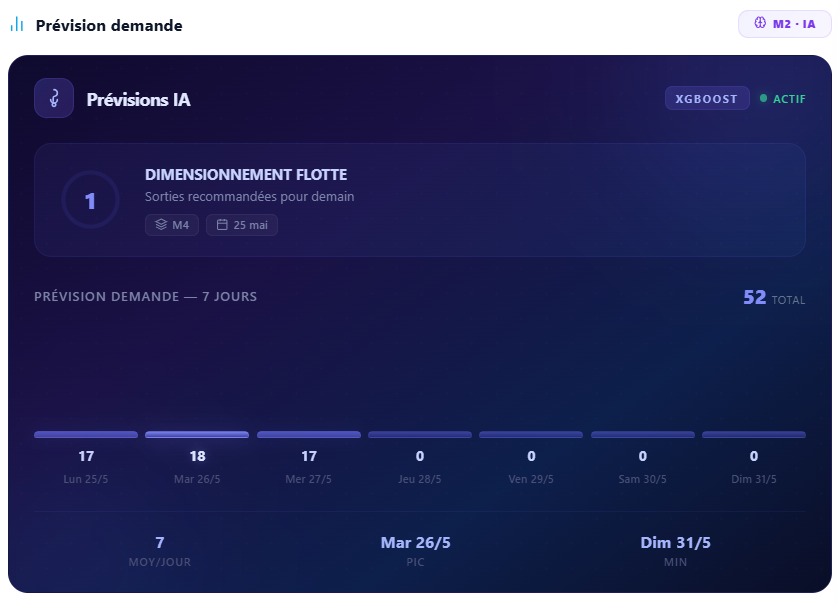
\includegraphics[width=\linewidth, keepaspectratio]{img/capture/ai/sp5_m2_demand_forecast_composite}%
}{%
  \fbox{\parbox{0.9\linewidth}{\centering\vspace{4cm}\textit{[\`{}img/sp5\_m2\_demand\_forecast\_composite\`{} --- Capture à réaliser]}\vspace{4cm}}}%
}
\caption{Intégration M2 Demand Forecast : tableau de bord Planificateur avec graphique de prévision de la demande par zone sur 7~jours}
\label{fig:sp5-m2-integration}
\end{figure}

\subsubsection{M3 -- Delay Prediction}

\begin{figure}[H]
\centering
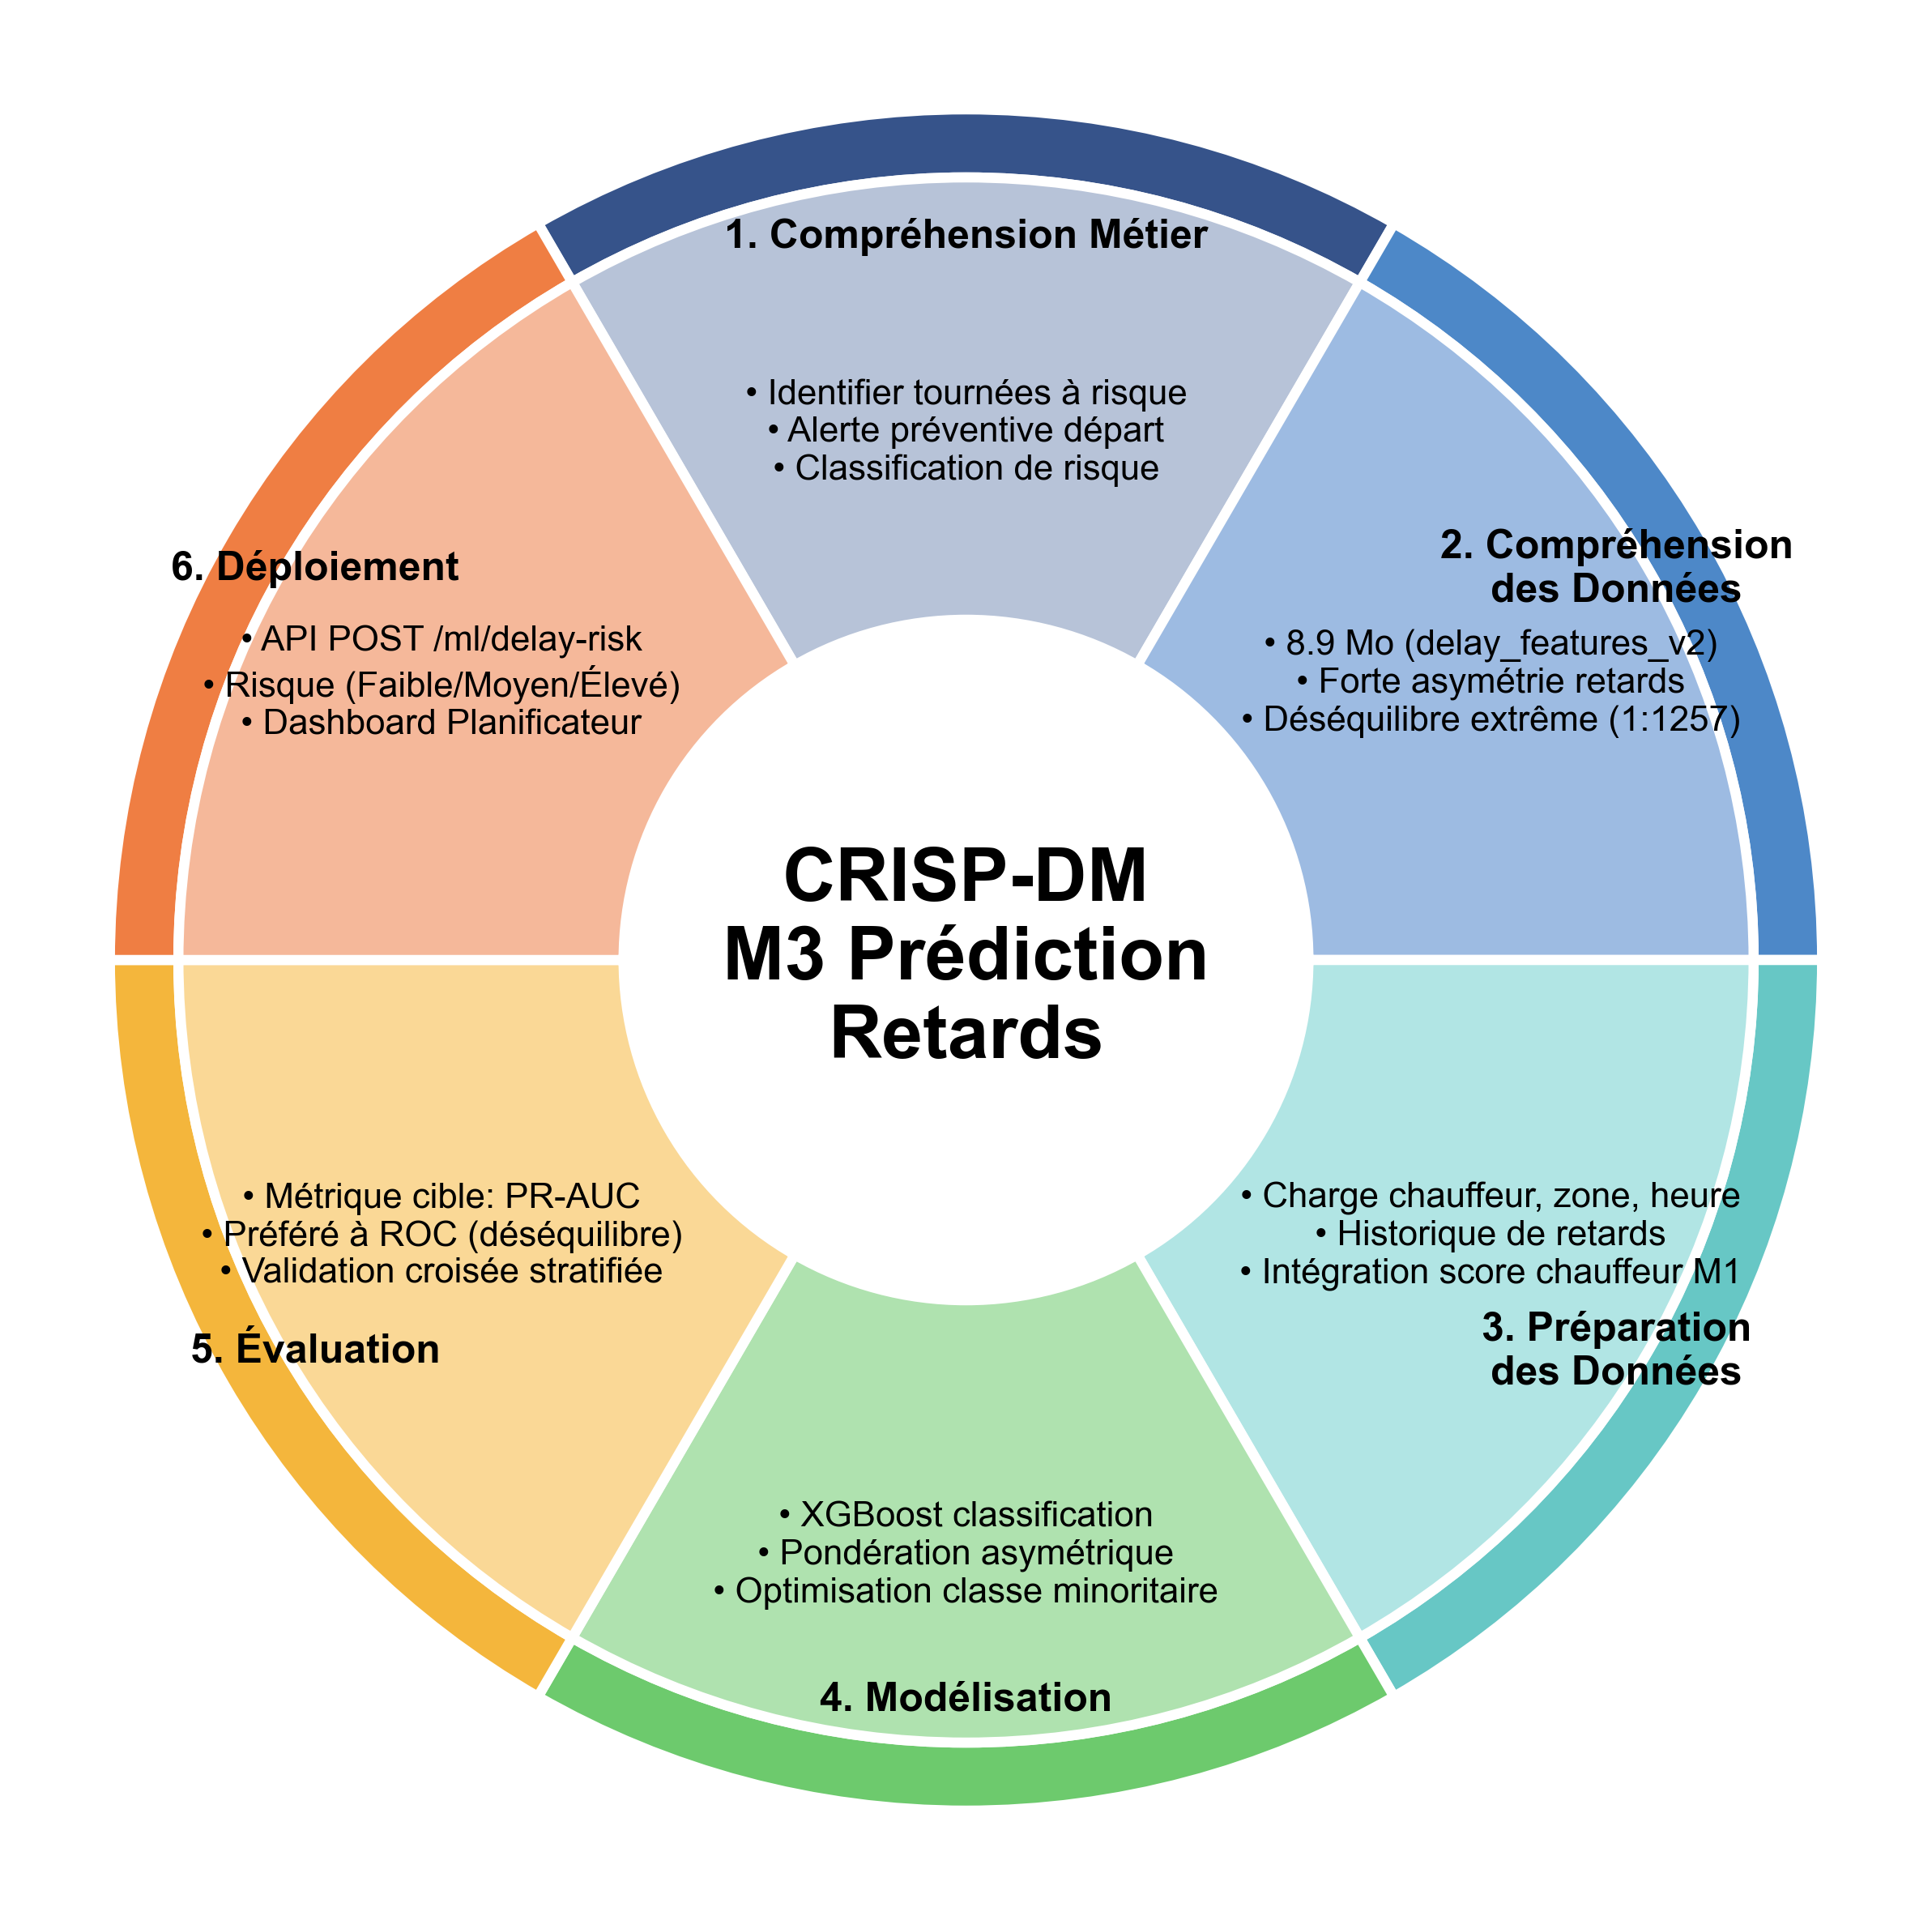
\includegraphics[width=0.88\linewidth]{img/crisp/crisp_dm_m3_delay}
\caption{Diagramme CRISP-DM -- M3 Prédiction des Retards}
\label{fig:crisp-m3}
\end{figure}

\begin{table}[H]
\centering
\setlength{\arrayrulewidth}{1pt}
\begin{tabular}{|p{3.5cm}|p{9.5cm}|}
\hline
\rowcolor{headerbg}
\multicolumn{2}{|c|}{\textbf{M3 -- Delay Prediction}} \\
\hline
\textbf{Objectif métier} & Identifier les tournées à risque de retard avant leur départ pour intervention préventive. \\
\hline
\textbf{Dataset} & \texttt{delay\_features\_v2.parquet} (8,9~Mo) \\
\hline
\textbf{Features clés} & Charge du chauffeur, zone, heure de départ, historique de retards, score M1. \\
\hline
\textbf{Algorithme} & XGBoost classification, pondération asymétrique des coûts (déséquilibre 1:1257). \\
\hline
\textbf{Métrique cible} & PR-AUC (plus représentative que ROC sur classes déséquilibrées). \\
\hline
\textbf{Intégration} & Indicateur de risque (Faible / Moyen / Élevé) dans le tableau de bord Planificateur. \\
\hline
\end{tabular}
\caption{Fiche synthétique -- M3 Delay Prediction}
\label{tab:m3-summary}
\end{table}
\setlength{\arrayrulewidth}{0.4pt}

\paragraph{Intégration dans l'application.}
L'indicateur de risque de retard (Faible~/ Moyen~/ Élevé) est affiché en couleur sur chaque tournée du tableau de bord Planificateur, permettant une intervention préventive avant le départ.

\begin{figure}[H]
\centering
\IfFileExists{img/capture/ai/sp5_m3_delay_prediction_composite.png}{%
  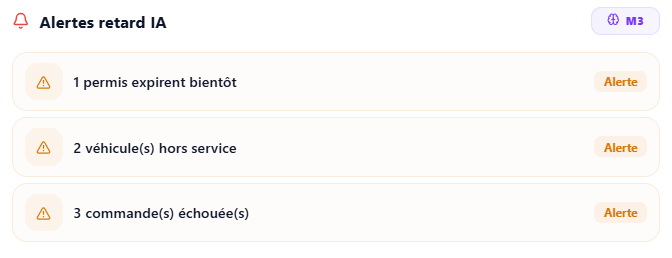
\includegraphics[width=\linewidth, keepaspectratio]{img/capture/ai/sp5_m3_delay_prediction_composite}%
}{%
  \fbox{\parbox{0.9\linewidth}{\centering\vspace{4cm}\textit{[\`{}img/sp5\_m3\_delay\_prediction\_composite\`{} --- Capture à réaliser]}\vspace{4cm}}}%
}
\caption{Intégration M3 Delay Prediction : indicateur de risque de retard (Faible / Moyen / Élevé) dans le tableau de bord Planificateur}
\label{fig:sp5-m3-integration}
\end{figure}

\subsubsection{M4 -- Fleet Dimensioning}

\begin{figure}[H]
\centering
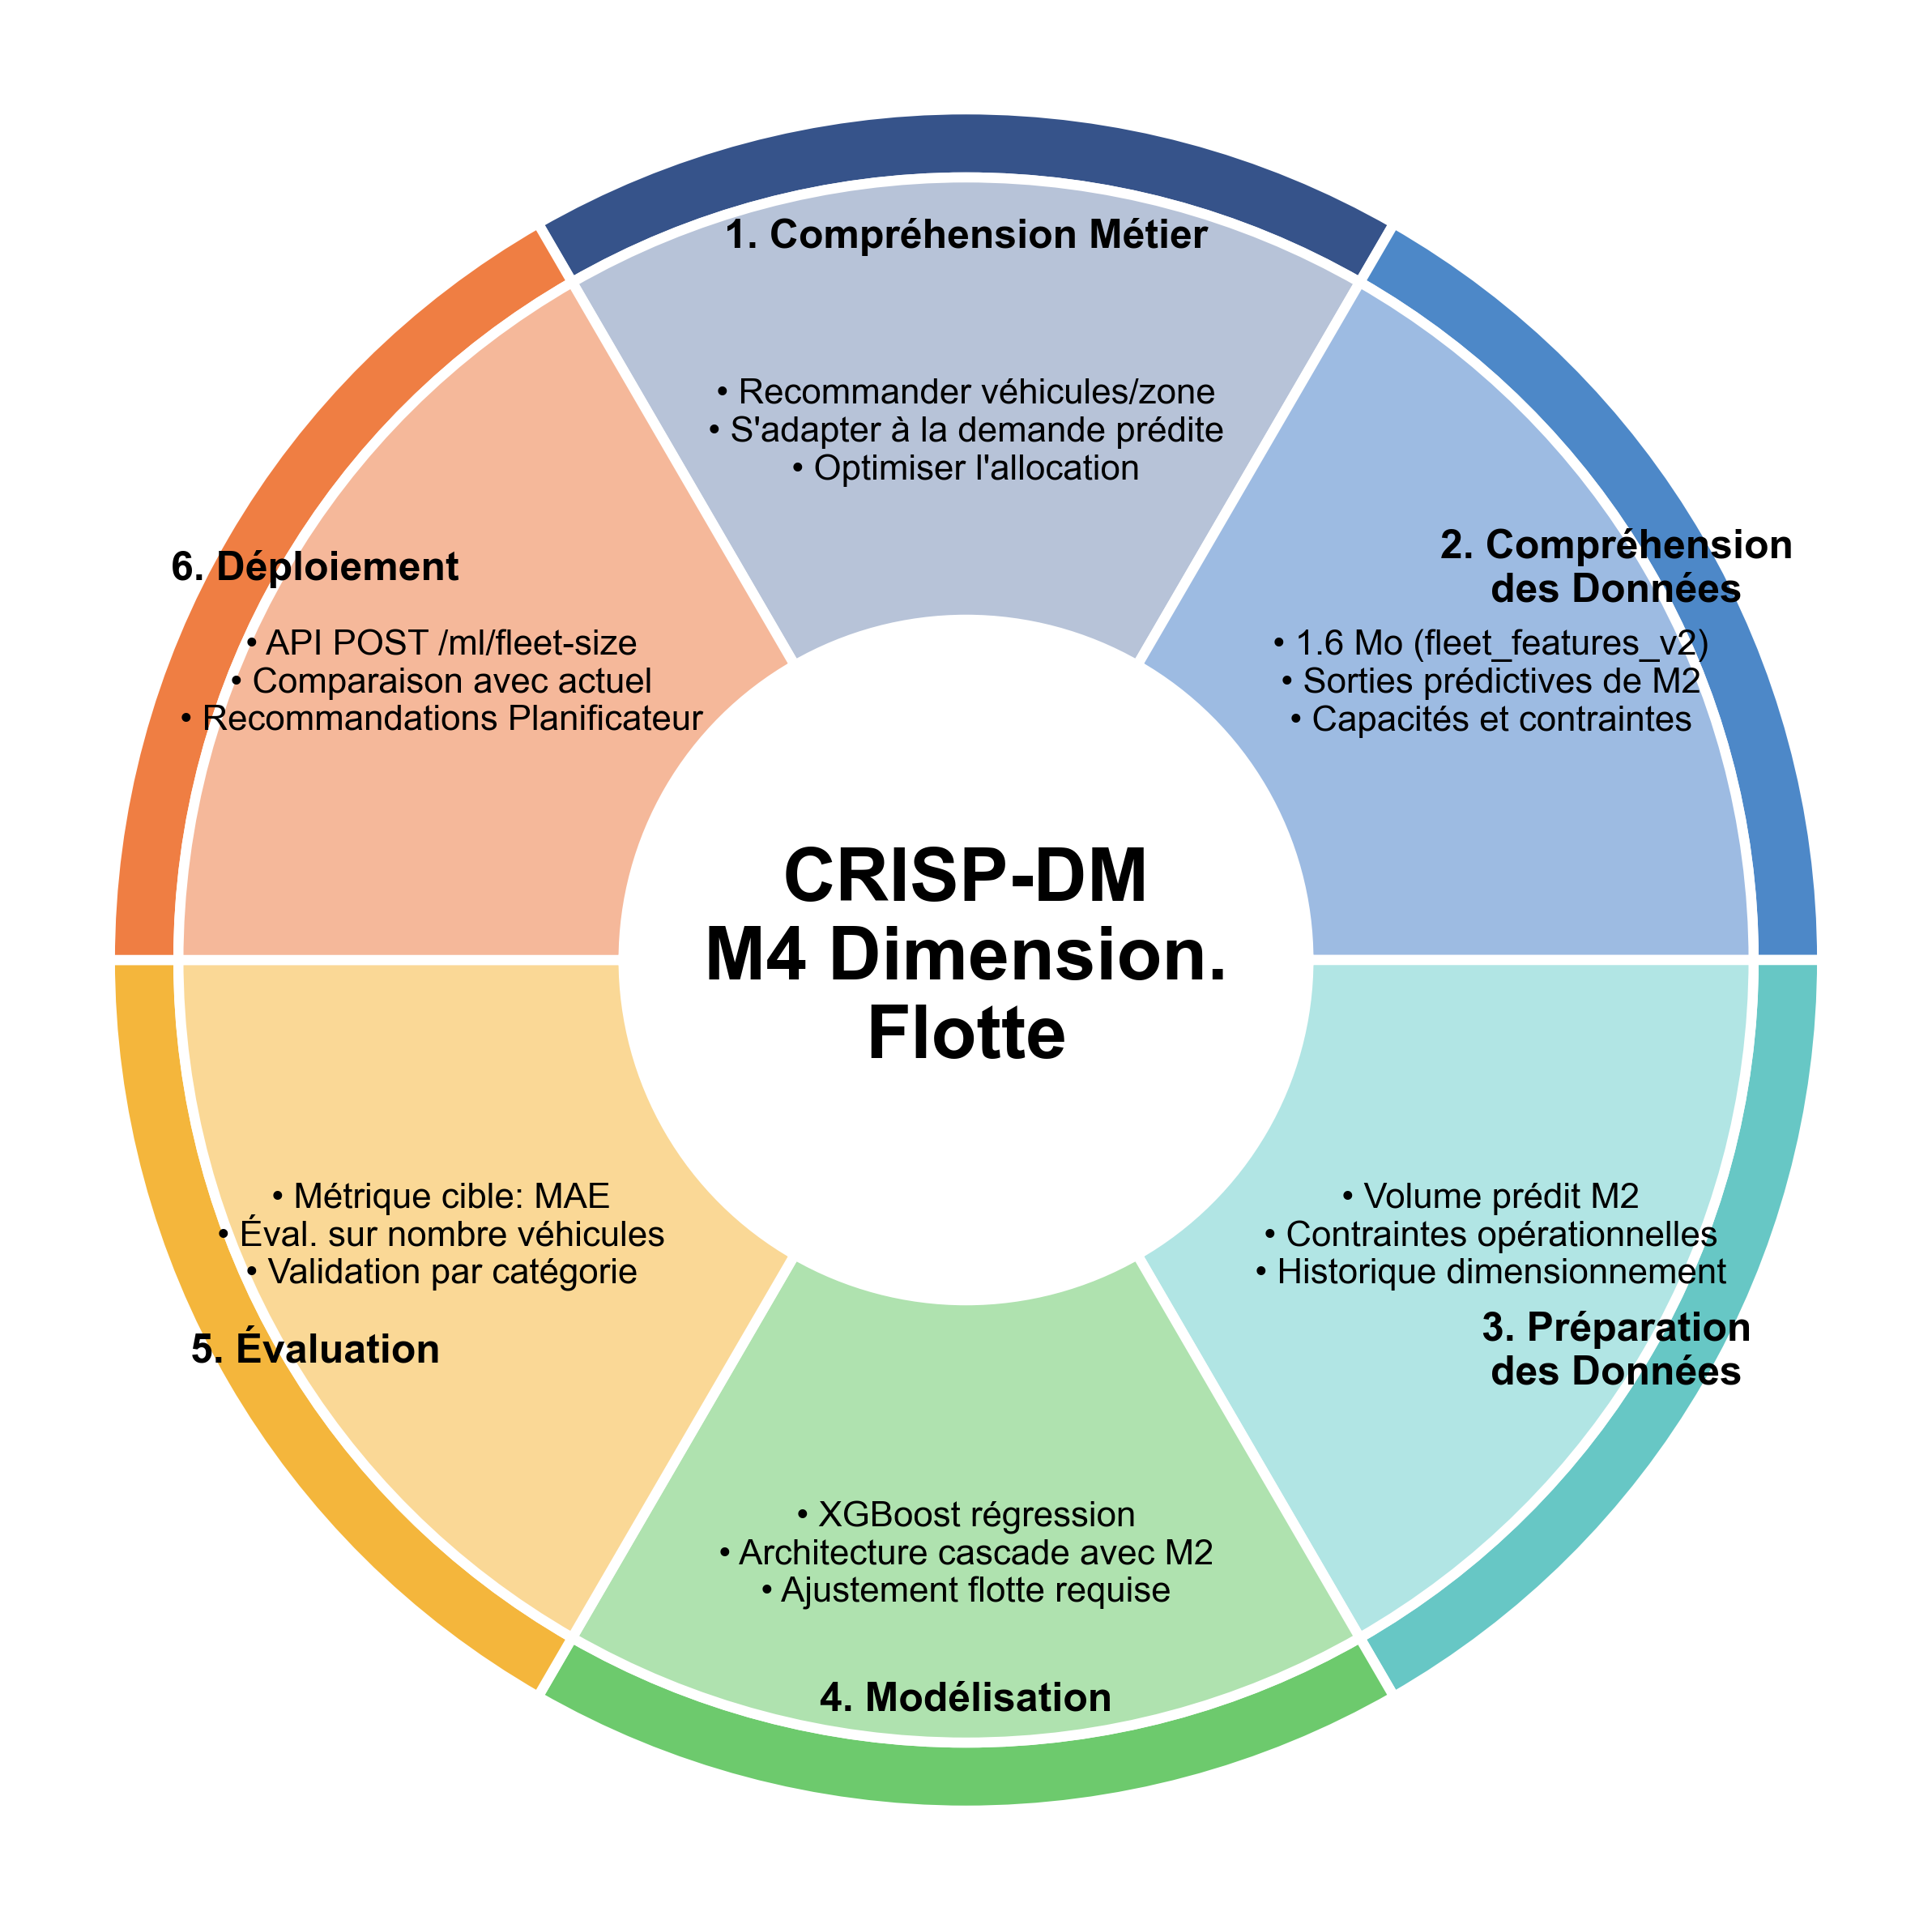
\includegraphics[width=0.88\linewidth]{img/crisp/crisp_dm_m4_fleet}
\caption{Diagramme CRISP-DM -- M4 Dimensionnement de Flotte}
\label{fig:crisp-m4}
\end{figure}

\begin{table}[H]
\centering
\setlength{\arrayrulewidth}{1pt}
\begin{tabular}{|p{3.5cm}|p{9.5cm}|}
\hline
\rowcolor{headerbg}
\multicolumn{2}{|c|}{\textbf{M4 -- Fleet Dimensioning}} \\
\hline
\textbf{Objectif métier} & Recommander le nombre optimal de véhicules par zone selon la demande prédite. \\
\hline
\textbf{Dataset} & \texttt{fleet\_features\_v2.parquet} (1,6~Mo) + sorties M2 (cascade). \\
\hline
\textbf{Features clés} & Volume prédit M2, capacité véhicule, contraintes opérationnelles, historique de dimensionnement. \\
\hline
\textbf{Algorithme} & XGBoost régression régularisée, architecture en cascade avec M2. \\
\hline
\textbf{Métrique cible} & MAE sur le nombre de véhicules recommandés. \\
\hline
\textbf{Intégration} & Recommandations de flotte dans le tableau de bord Planificateur avec comparaison flotte actuelle. \\
\hline
\end{tabular}
\caption{Fiche synthétique -- M4 Fleet Dimensioning}
\label{tab:m4-summary}
\end{table}
\setlength{\arrayrulewidth}{0.4pt}

\paragraph{Intégration dans l'application.}
Les recommandations de dimensionnement de flotte (nombre optimal de véhicules par zone) sont affichées dans le tableau de bord Planificateur avec une comparaison visuelle par rapport à la flotte actuelle.

\begin{figure}[H]
\centering
\IfFileExists{img/capture/ai/sp5_m4_fleet_sizing_composite.png}{%
  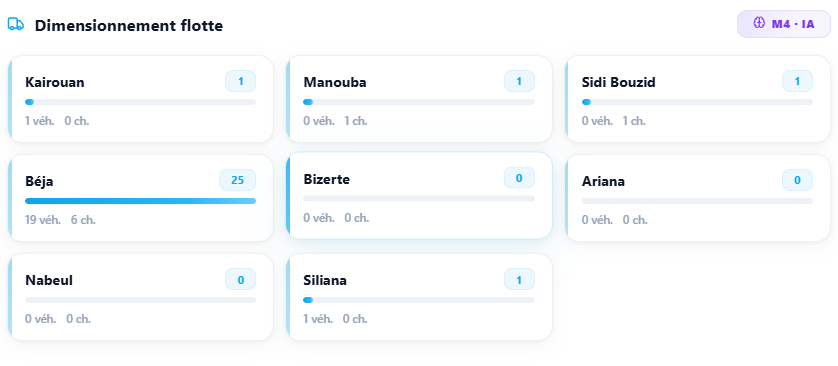
\includegraphics[width=\linewidth, keepaspectratio]{img/capture/ai/sp5_m4_fleet_sizing_composite}%
}{%
  \fbox{\parbox{0.9\linewidth}{\centering\vspace{4cm}\textit{[\`{}img/sp5\_m4\_fleet\_sizing\_composite\`{} --- Capture à réaliser]}\vspace{4cm}}}%
}
\caption{Intégration M4 Fleet Dimensioning : recommandations de dimensionnement de flotte par zone, comparaison avec la flotte actuelle}
\label{fig:sp5-m4-integration}
\end{figure}

\subsubsection{M5 -- Route Learning}

\begin{figure}[H]
\centering
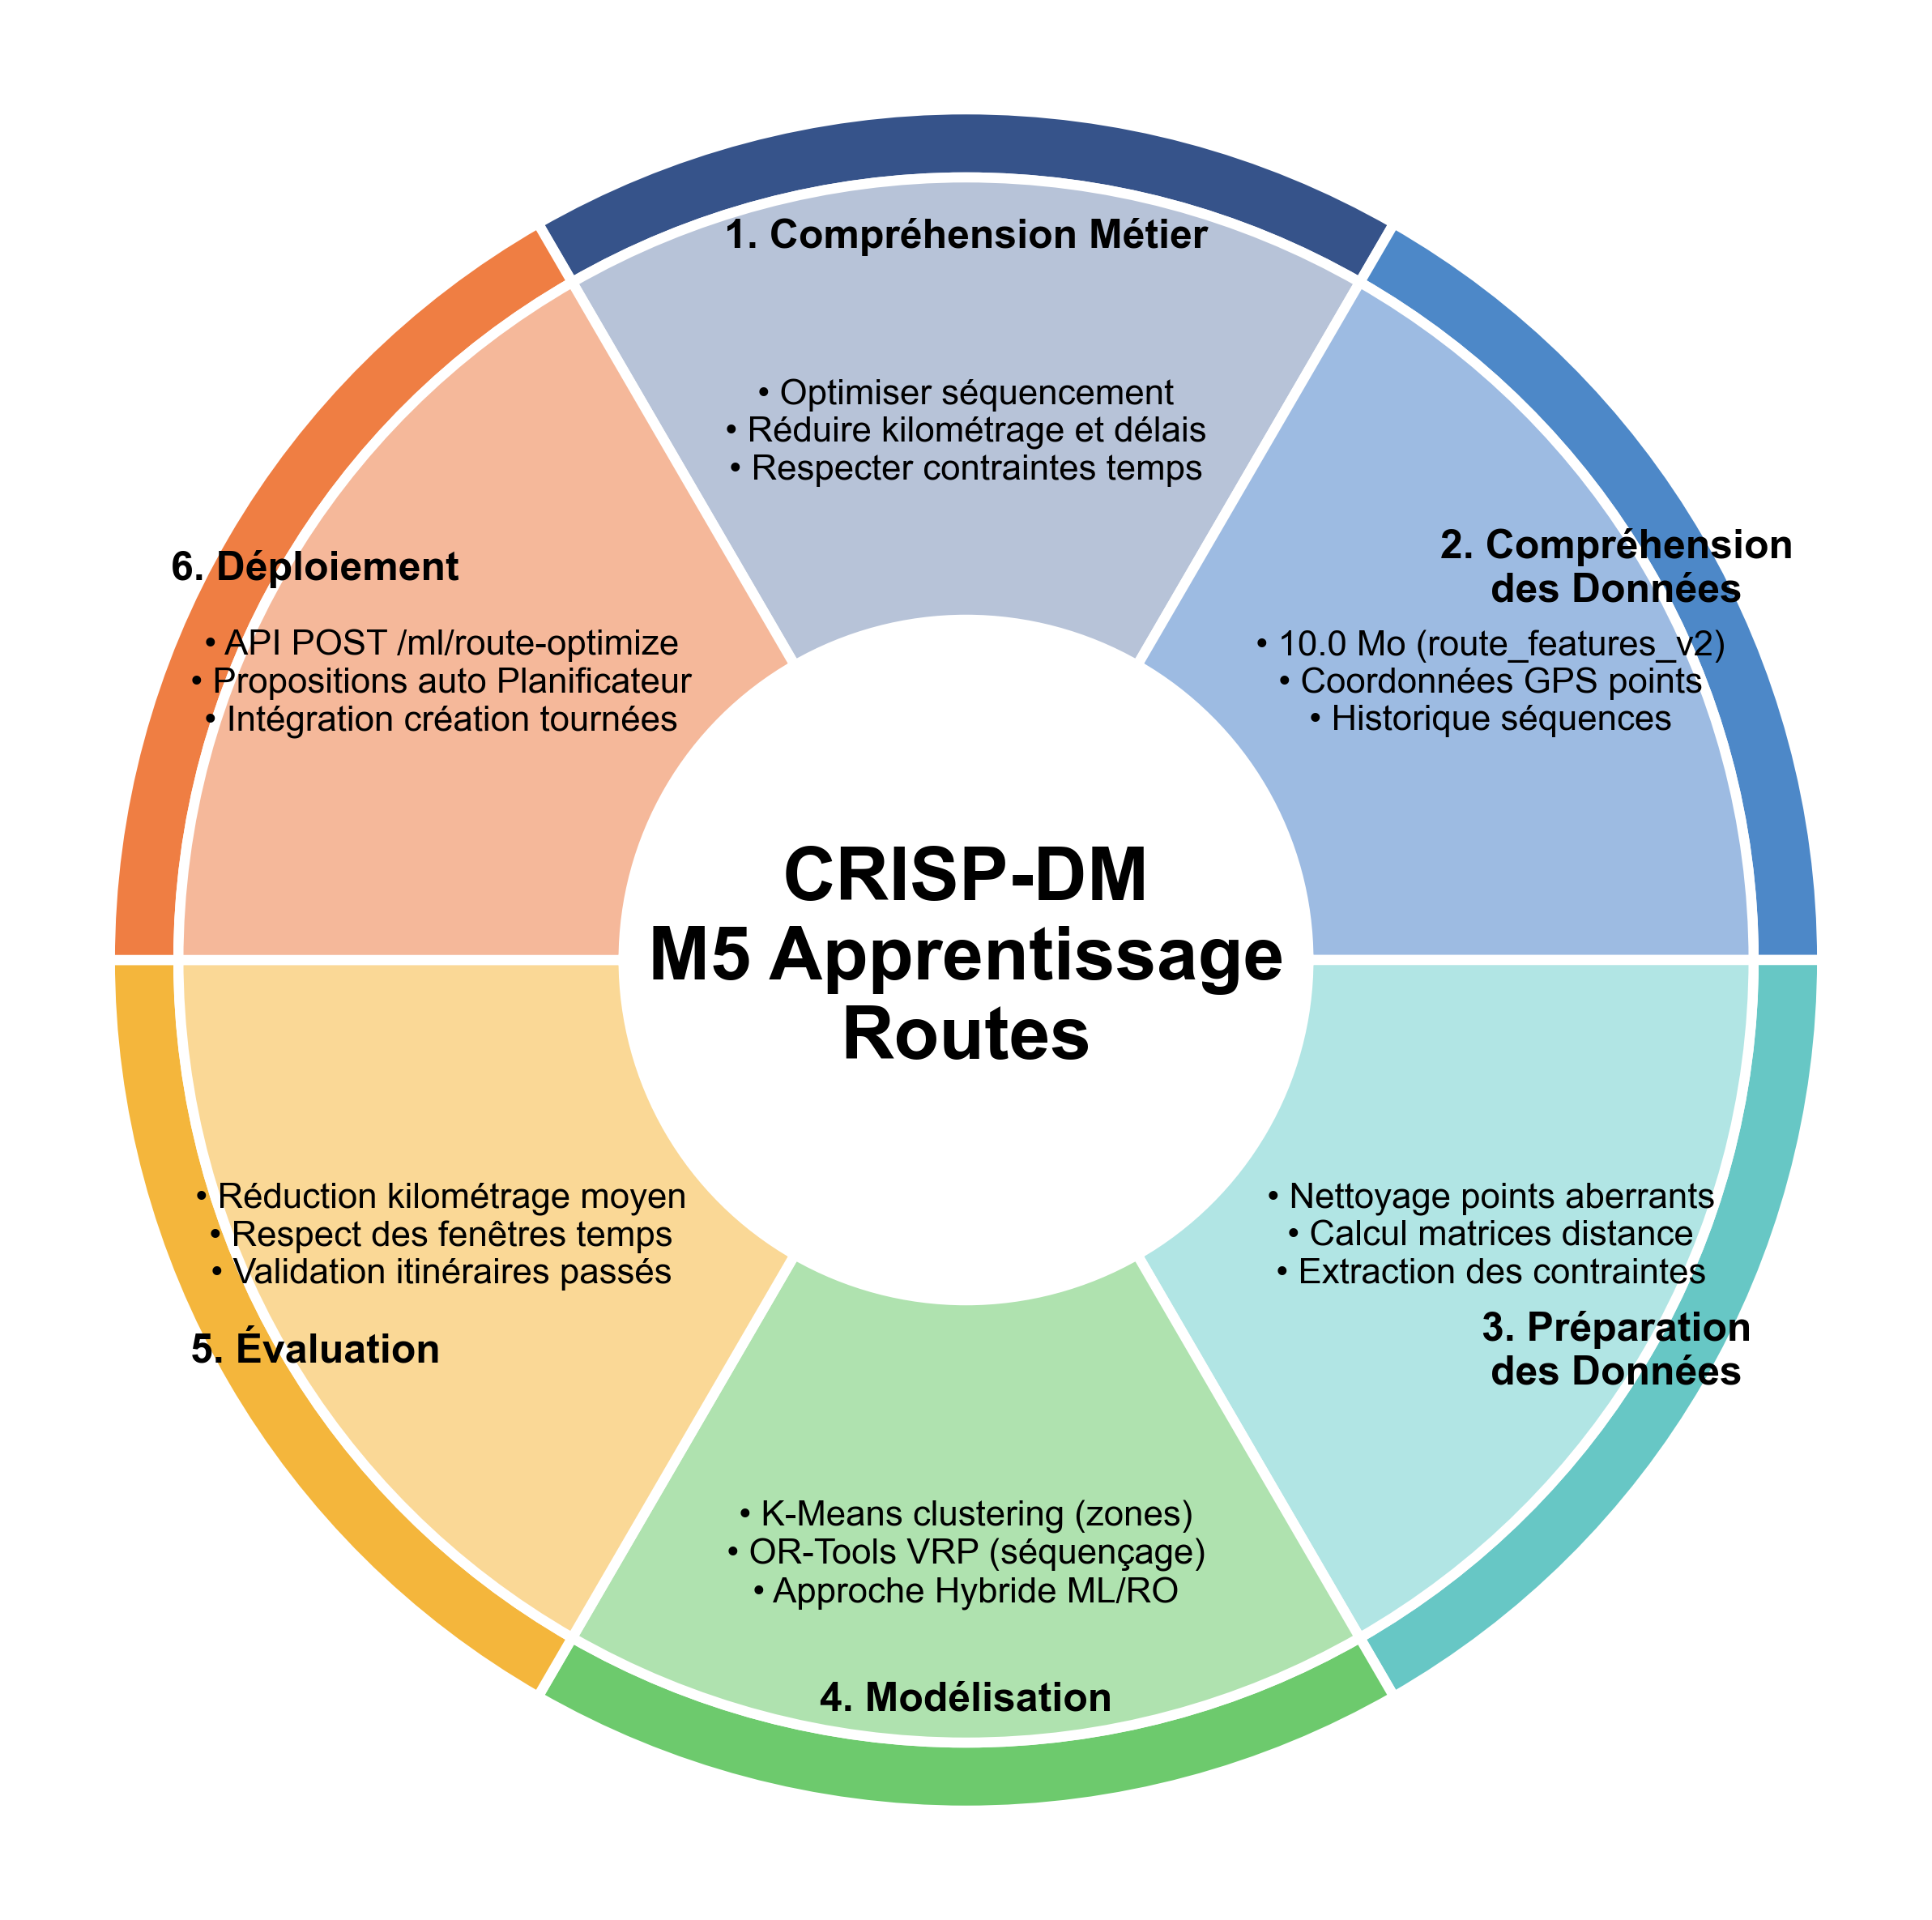
\includegraphics[width=0.88\linewidth]{img/crisp/crisp_dm_m5_route}
\caption{Diagramme CRISP-DM -- M5 Apprentissage des Routes}
\label{fig:crisp-m5}
\end{figure}

\begin{table}[H]
\centering
\setlength{\arrayrulewidth}{1pt}
\begin{tabular}{|p{3.5cm}|p{9.5cm}|}
\hline
\rowcolor{headerbg}
\multicolumn{2}{|c|}{\textbf{M5 -- Route Learning}} \\
\hline
\textbf{Objectif métier} & Optimiser le séquencement des tournées pour réduire le kilométrage et les délais. \\
\hline
\textbf{Dataset} & \texttt{route\_features\_v2.parquet} (10,0~Mo) \\
\hline
\textbf{Features clés} & Coordonnées GPS, historique de séquences efficaces, contraintes de temps, capacité. \\
\hline
\textbf{Algorithme} & Hybride : K-Means clustering (partitionnement de zones) + OR-Tools VRP (optimisation de séquence). \\
\hline
\textbf{Métrique cible} & Réduction du kilométrage moyen par tournée. \\
\hline
\textbf{Intégration} & Routes optimisées proposées au Planificateur lors de la création de tournées. \\
\hline
\end{tabular}
\caption{Fiche synthétique -- M5 Route Learning}
\label{tab:m5-summary}
\end{table}
\setlength{\arrayrulewidth}{0.4pt}

\paragraph{Modélisation et justification du modèle.}
Contrairement aux modèles prédictifs classiques (comme XGBoost utilisé pour le scoring), l'apprentissage des routes est un problème complexe d'optimisation combinatoire (VRP -- \textit{Vehicle Routing Problem}). Cinq approches algorithmiques ont été évaluées lors de cette phase. Les résultats obtenus sur un jeu de test de 500 tournées historiques sont présentés dans le tableau~\ref{tab:m5-evaluation}.

\begin{table}[H]
\centering
\setlength{\arrayrulewidth}{1pt}
\begin{tabular}{|l|c|c|p{4cm}|}
\hline
\rowcolor{headerbg}
\textbf{Algorithme} & \textbf{Écart à l'optimal (Gap)} & \textbf{Respect des délais} & \textbf{Temps d'exécution moyen} \\
\hline
Heuristique d'insertion & 14,5\,\% & 72\,\% & Très rapide (< 1 s) \\
\hline
Algorithme Génétique & 8,2\,\% & 84\,\% & Très lent ($\approx$ 5 min) \\
\hline
Recuit Simulé & 6,8\,\% & 87\,\% & Lent ($\approx$ 3 min) \\
\hline
OptaPlanner (Tabu Search) & 3,4\,\% & 94\,\% & Moyen ($\approx$ 1 min) \\
\hline
\textbf{K-Means + OR-Tools} & \textbf{1,2\,\%} & \textbf{98\,\%} & \textbf{Rapide ($\approx$ 10 s)} \\
\hline
\end{tabular}
\caption{Comparatif des algorithmes évalués pour le modèle M5 (Optimisation VRP)}
\label{tab:m5-evaluation}
\end{table}
\setlength{\arrayrulewidth}{0.4pt}

L'approche hybride \textbf{K-Means + OR-Tools} a été retenue. En premier lieu, l'algorithme K-Means pré-partitionne géographiquement les points de livraison (Clustering spatial), ce qui réduit drastiquement l'espace de recherche. Ensuite, le solveur OR-Tools de Google applique des heuristiques de routage avancées (\textit{Guided Local Search}) sur chaque cluster. En plus de garantir le meilleur respect des contraintes de temps (98\,\%), cette combinaison offre le compromis idéal entre la qualité de la solution (écart minimal de 1,2\,\%) et un temps d'exécution très court (10 secondes), une exigence fondamentale pour les planificateurs de PGH.

\paragraph{Intégration dans l'application.}
Les routes optimisées par M5 sont proposées au Planificateur sous forme de suggestions d'itinéraires dans l'interface de planification. Le Planificateur peut accepter, modifier ou rejeter chaque suggestion avec traitement de la rétroaction (\texttt{SuggestionIA.decision}).

\begin{figure}[H]
\centering
\IfFileExists{img/capture/ai/sp5_m5_route_suggestions_composite.png}{%
  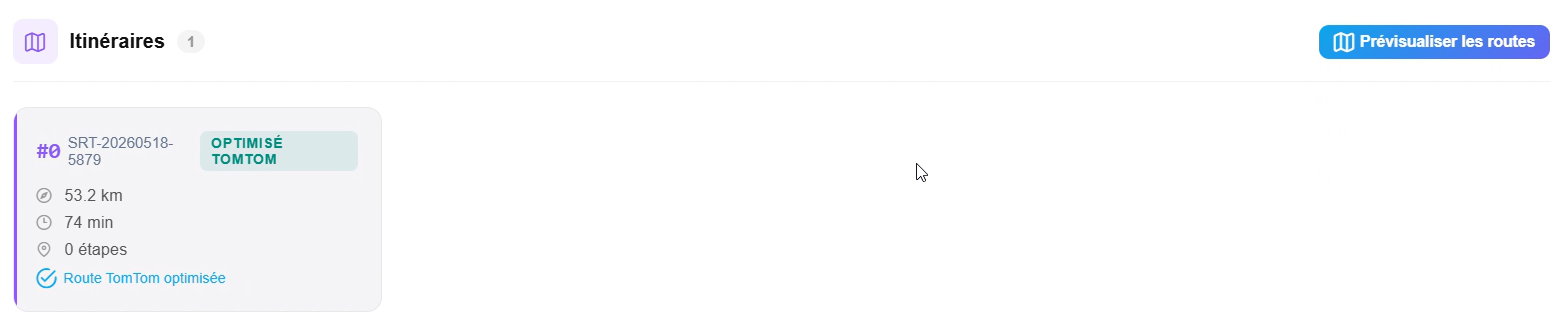
\includegraphics[width=\linewidth, keepaspectratio]{img/capture/ai/sp5_m5_route_suggestions_composite}%
}{%
  \fbox{\parbox{0.9\linewidth}{\centering\vspace{4cm}\textit{[\`{}img/sp5\_m5\_route\_suggestions\_composite\`{} --- Capture à réaliser]}\vspace{4cm}}}%
}
\caption{Intégration M5 Route Learning : interface suggestions d'itinéraires optimisés (K-Means + OR-Tools), score de qualité et actions Accepter / Modifier / Rejeter}
\label{fig:sp5-m5-integration}
\end{figure}

\subsubsection{M6 -- Payment Risk}

\begin{figure}[H]
\centering
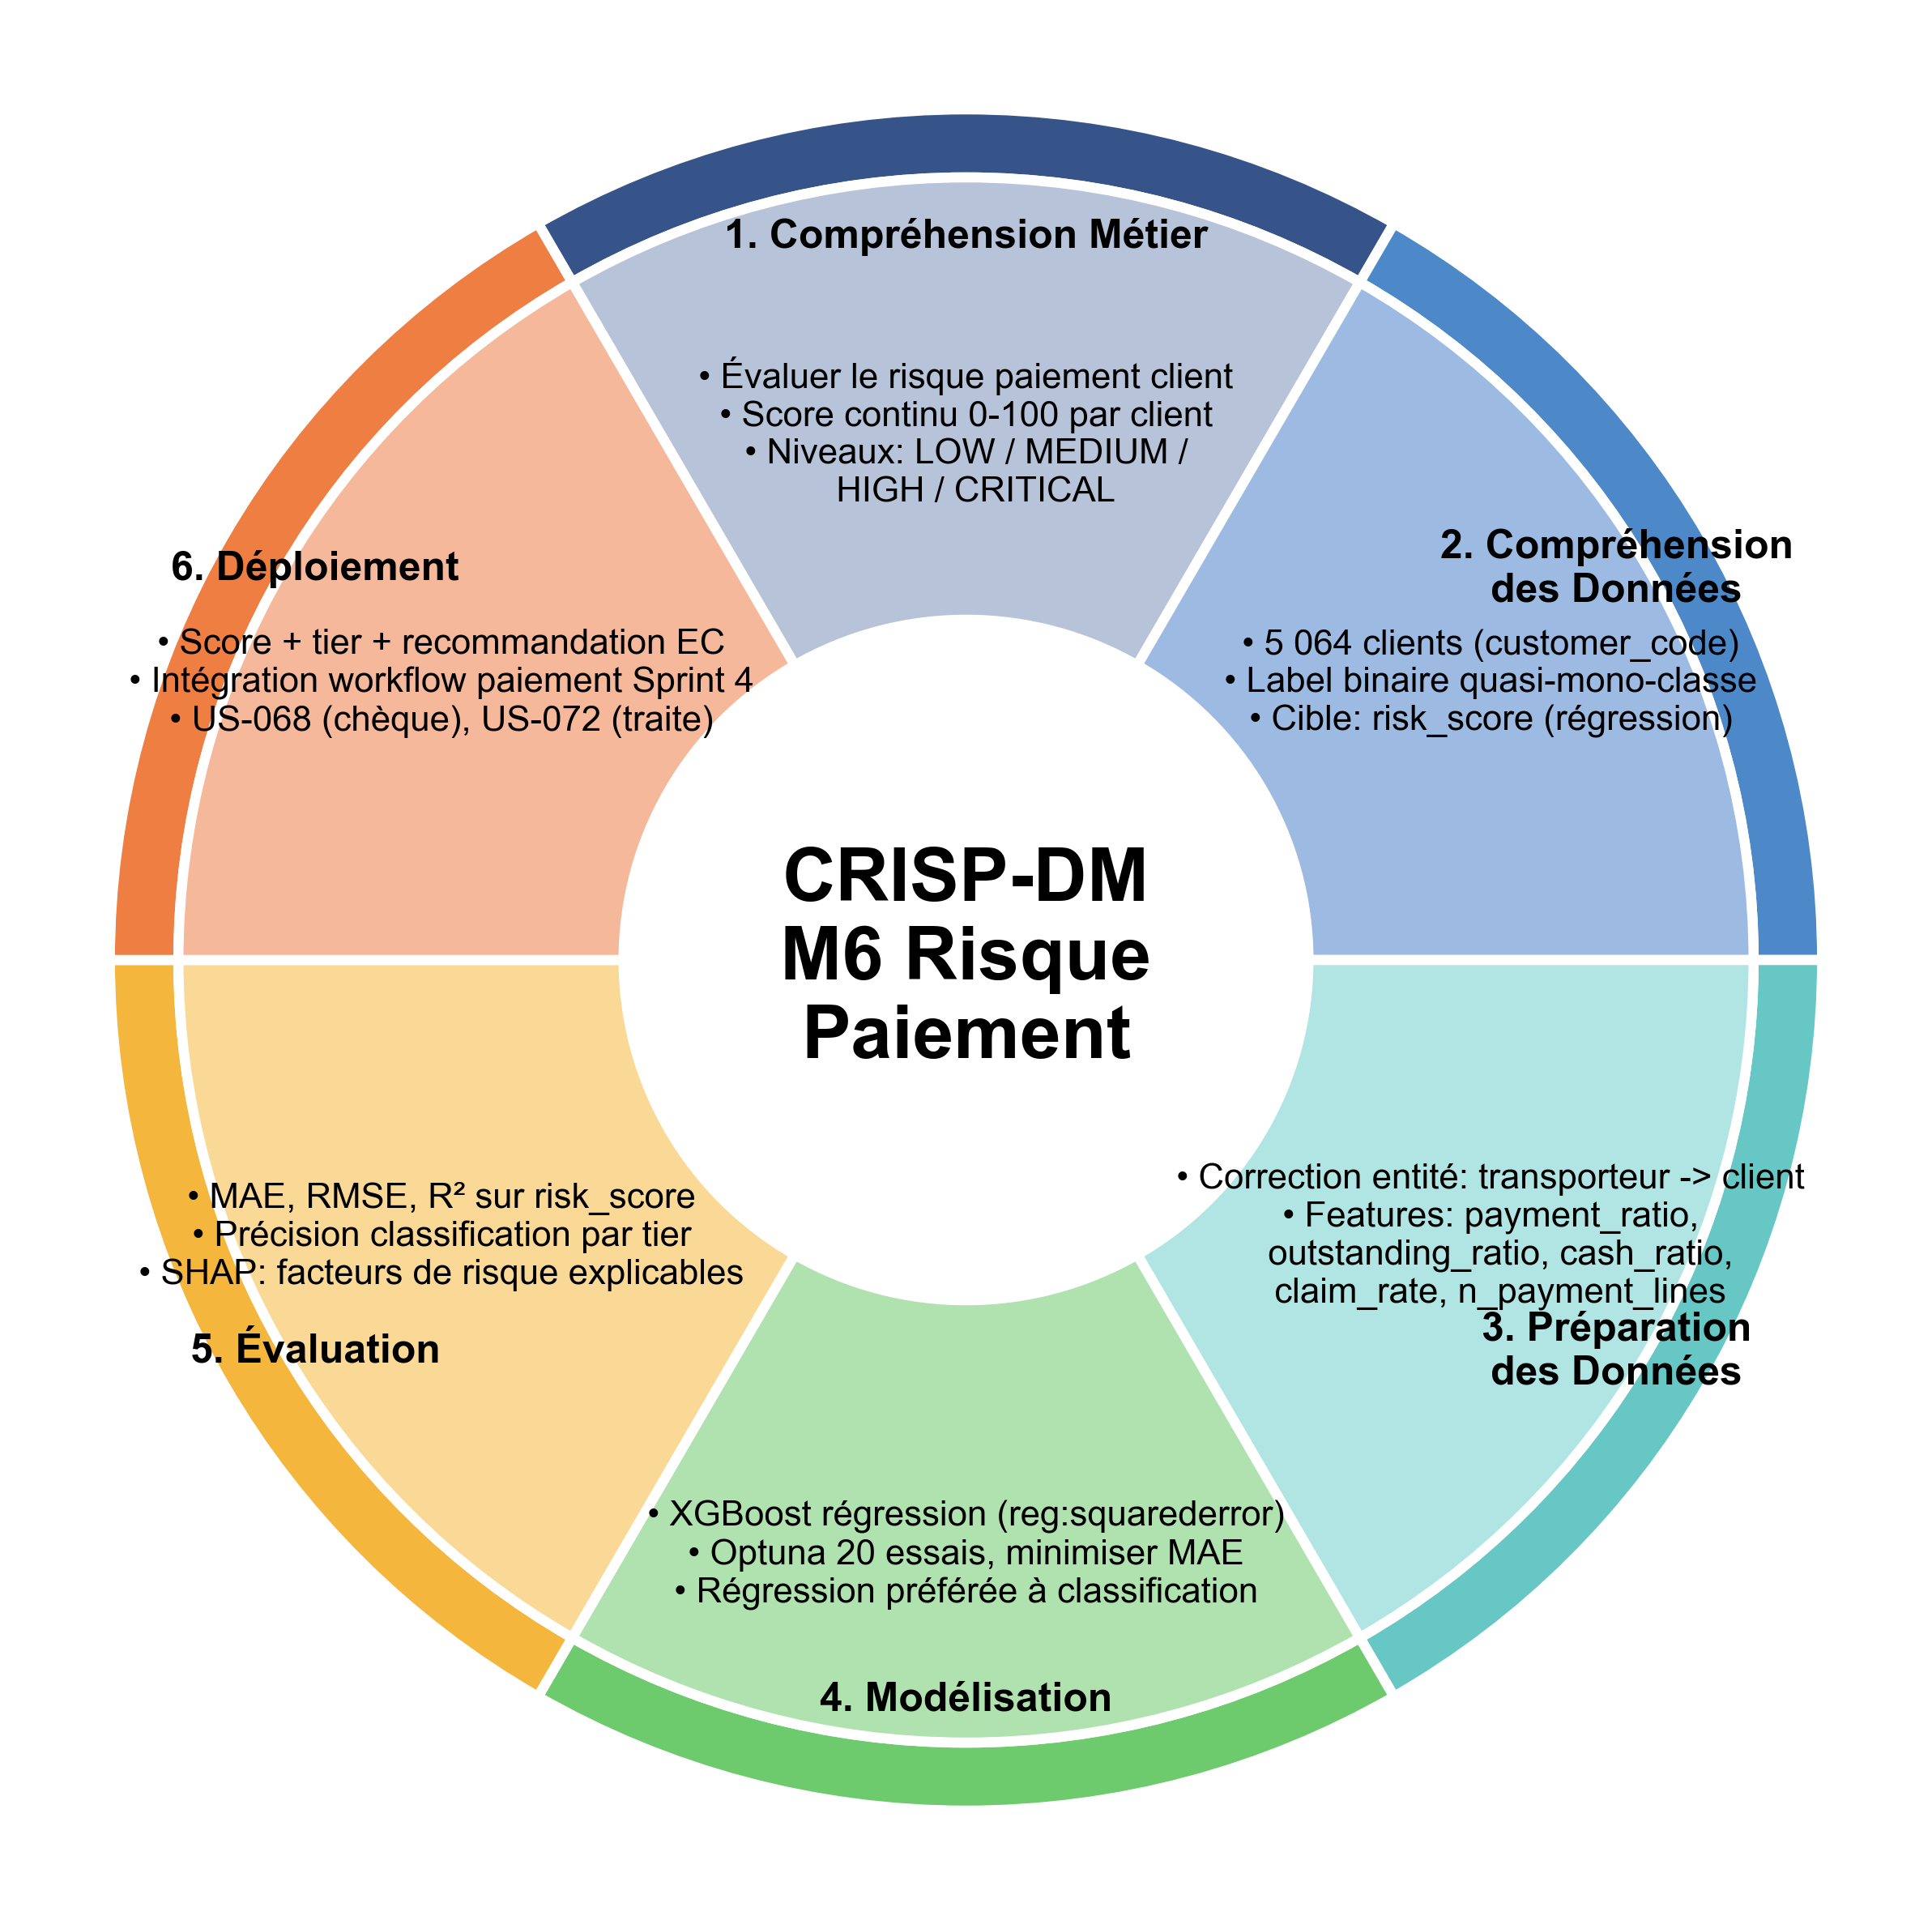
\includegraphics[width=0.88\linewidth]{img/crisp/crisp_dm_m6_payment}
\caption{Diagramme CRISP-DM -- M6 Risque Paiement Client}
\label{fig:crisp-m6}
\end{figure}

\begin{table}[H]
\centering
\setlength{\arrayrulewidth}{1pt}
\begin{tabular}{|p{3.5cm}|p{9.5cm}|}
\hline
\rowcolor{headerbg}
\multicolumn{2}{|c|}{\textbf{M6 -- Payment Risk}} \\
\hline
\textbf{Objectif métier} & Évaluer la solvabilité opérationnelle d'un client pour décider du mode de paiement autorisé. \\
\hline
\textbf{Dataset} & \texttt{payment\_risk\_v2.parquet} (0,3~Mo) \\
\hline
\textbf{Features clés} & Historique de paiements, taux d'incidents, ancienneté client, volume de commandes, délais de règlement. \\
\hline
\textbf{Algorithme} & XGBoost régression, score normalisé 0--100, seuils : Low / Medium / High / Critical. \\
\hline
\textbf{Métrique cible} & Corrélation entre score prédit et incidents de paiement réels. \\
\hline
\textbf{Intégration} & Score de risque visible par le REC lors de la validation d'une commande ou d'un paiement par traite. \\
\hline
\end{tabular}
\caption{Fiche synthétique -- M6 Payment Risk}
\label{tab:m6-summary}
\end{table}
\setlength{\arrayrulewidth}{0.4pt}

\paragraph{Intégration dans l'application.}
Le score de risque paiement (Low~/ Medium~/ High~/ Critical) est affiché par le REC lors de la validation d'une commande ou d'un paiement par traite, permettant une décision d'octroi de crédit informatisée.

\begin{figure}[H]
\centering
\IfFileExists{img/capture/ai/sp5_m6_payment_risk_composite.png}{%
  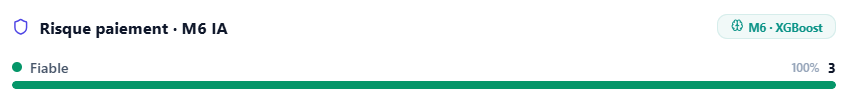
\includegraphics[width=\linewidth, keepaspectratio]{img/capture/ai/sp5_m6_payment_risk_composite}%
}{%
  \fbox{\parbox{0.9\linewidth}{\centering\vspace{4cm}\textit{[\`{}img/sp5\_m6\_payment\_risk\_composite\`{} --- Capture à réaliser]}\vspace{4cm}}}%
}
\caption{Intégration M6 Payment Risk : score de risque paiement (Low / Medium / High / Critical) affiché au REC lors de la validation d'une commande}
\label{fig:sp5-m6-integration}
\end{figure}

\subsubsection{Tableau comparatif des six modèles}

\begin{table}[H]
\centering
\setlength{\arrayrulewidth}{1pt}
\resizebox{\textwidth}{!}{%
\begin{tabular}{|l|l|l|l|l|}
\hline
\rowcolor{headerbg}
\textbf{Modèle} & \textbf{Type} & \textbf{Algorithme} & \textbf{Métrique} & \textbf{Endpoint FastAPI} \\
\hline
M1 Driver Scoring & Classification & XGBoost & F1 / AUC-ROC & \texttt{/ml/driver-score} \\
\hline
M2 Demand Forecast & Régression multi & XGBoost & MAPE $<$15\,\% & \texttt{/ml/demand-forecast} \\
\hline
M3 Delay Prediction & Classification & XGBoost & PR-AUC & \texttt{/ml/delay-risk} \\
\hline
M4 Fleet Sizing & Régression & XGBoost (cascade) & MAE & \texttt{/ml/fleet-size} \\
\hline
M5 Route Learning & Clustering + VRP & K-Means + OR-Tools & km réduit & \texttt{/ml/route-optimize} \\
\hline
M6 Payment Risk & Régression & XGBoost & Score 0--100 & \texttt{/ml/payment-risk} \\
\hline
\end{tabular}%
}
\caption{Comparatif des six modèles ML déployés dans Fleet~AI}
\label{tab:ml-comparatif}
\end{table}
\setlength{\arrayrulewidth}{0.4pt}

% -----------------------------------------------------------
\subsection{Architecture LLM et Chatbot Text-to-SQL}
% -----------------------------------------------------------

Fleet~AI intègre un chatbot analytique fondé sur le modèle \textbf{Gemma~4 31B} déployé localement via \textbf{Ollama}. L'utilisateur interroge la base de données en langage naturel ; le système génère, valide et exécute la requête SQL correspondante, puis reformule le résultat en texte. Ce déploiement on-premise est une contrainte métier : PGH ne peut pas externaliser ses données opérationnelles vers des API cloud tierces.

\subsubsection{Architecture globale}

% ============================================================
% FIGURE 8.8 — Architecture Text-to-SQL locale
% ============================================================
%
%  Layout (3 couches horizontales, pipeline en Z) :
%
%  ┌─────────────────────────── Frontend ──────────────────────┐
%  │  [Utilisateur]                                            │
%  └───────────────────────────────────────────────────────────┘
%  ┌─────────────────────────── Backend ───────────────────────┐
%  │  (1)Auth → (2)Session → (3)Intention → (4)Génération SQL  │
%  │                                              ↓            │
%  │  (7)Reformulation ← (6)Exécution ← (5)Validation         │
%  └───────────────────────────────────────────────────────────┘
%  ┌──────────────────── Infrastructure On-Premise ────────────┐
%  │  Redis/MongoDB     Ollama LLM      PostgreSQL  Schéma.md  │
%  └───────────────────────────────────────────────────────────┘
%
%  Règles de routage sans croisement :
%  • Pipeline principal : flèches bleues horizontales dans chaque rangée
%  • Retour (7)→Utilisateur : monte à gauche via couloir x=2.0
%  • Dépendances infra : flèches verticales directes
%    chaque nœud backend est aligné verticalement avec son infra
%
% ============================================================
% FIGURE 8.8 — Architecture Text-to-SQL locale
% ============================================================
\begin{figure}[H]
\centering
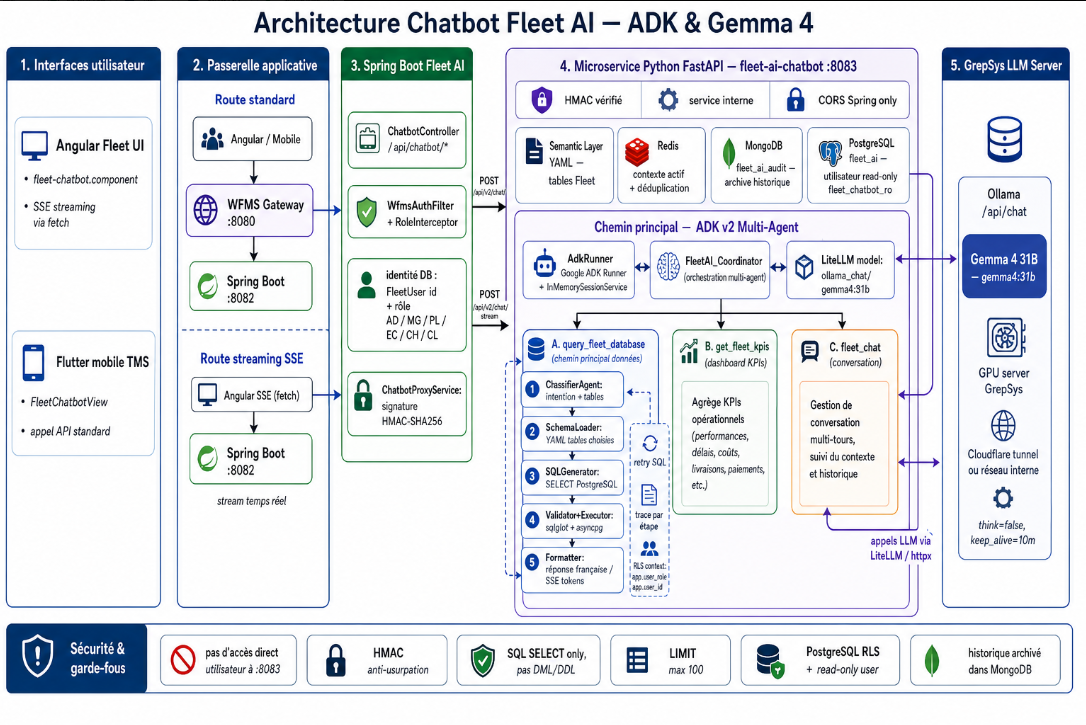
\includegraphics[width=\linewidth, keepaspectratio]{img/figure/chatBot}
\caption{Architecture Text-to-SQL locale --- Pipeline 7 étapes du Chatbot Fleet~AI (Gemma~4 31B via Ollama, déploiement on-premise PGH)}
\label{fig:dfd-chatbot}
\end{figure}


\subsubsection{Pipeline conversationnel}

Le traitement d'une requête utilisateur suit sept étapes :

\begin{enumerate}
  \item \textbf{Authentification et contexte} : la requête est reçue par le backend Spring Boot. L'identité et le rôle de l'utilisateur (RBAC) déterminent le périmètre de données accessible.
  \item \textbf{Gestion de session} : l'historique conversationnel est stocké dans \textbf{Redis} (TTL~30~min) pour maintenir le contexte entre les échanges successifs. Les conversations sont archivées dans \textbf{MongoDB}.
  \item \textbf{Compréhension de l'intention} : Gemma~4 31B analyse la question et identifie l'intention métier (reporting, agrégation, filtrage, tendance).
  \item \textbf{Génération SQL} : le LLM génère une requête SQL guidée par un \textit{schema prompt} injectant la structure relationnelle de Fleet~AI (tables, colonnes, relations).
  \item \textbf{Validation et sécurité} : un validateur intercepte la requête avant exécution -- blocage des instructions d'écriture (\texttt{INSERT}, \texttt{UPDATE}, \texttt{DELETE}), vérification syntaxique, contrôle des tables autorisées selon le rôle (RLS).
  \item \textbf{Exécution} : la requête validée s'exécute en lecture seule sur PostgreSQL.
  \item \textbf{Reformulation} : le jeu de résultats est retourné à Gemma~4 31B qui produit une réponse textuelle structurée, accessible depuis le frontend Angular (web) ou Flutter (mobile).
\end{enumerate}

\subsubsection{Sécurité et contraintes techniques}

\begin{table}[H]
\centering
\setlength{\arrayrulewidth}{1pt}
\begin{tabular}{|p{4cm}|p{9.5cm}|}
\hline
\rowcolor{headerbg}
\textbf{Composant} & \textbf{Rôle dans le pipeline} \\
\hline
Ollama & Serveur d'inférence local pour Gemma~4 31B. Aucune donnée ne quitte l'infrastructure PGH. \\
\hline
Redis & Cache de session conversationnelle (TTL configurable, éviction LRU). \\
\hline
MongoDB & Archivage persistant des conversations pour audit et ré-entraînement futur. \\
\hline
SQL Validator & Middleware Spring Boot : whitelist de tables, blocage DDL/DML, contrôle de la profondeur des jointures. \\
\hline
RLS (Row-Level Security) & Restriction PostgreSQL : chaque rôle ne voit que les données de son périmètre (zone, entreprise, tournée). \\
\hline
Spring Boot & Point d'entrée REST sécurisé (JWT), orchestrateur du pipeline multi-étapes. \\
\hline
\end{tabular}
\caption{Composants de l'architecture chatbot Text-to-SQL}
\label{tab:chatbot-components}
\end{table}
\setlength{\arrayrulewidth}{0.4pt}

\paragraph{Intégration dans l'application.}
L'interface de chatbot est accessible depuis le tableau de bord Manager (Angular) et depuis l'application mobile Flutter. L'utilisateur pose une question en français ou en arabe ; la réponse est affichée sous forme textuelle avec un tableau de données lorsque la question porte sur des agrégations ou des classements.

\begin{figure}[H]
\centering
\IfFileExists{img/capture/ai/sp5_chatbot_composite.png}{%
  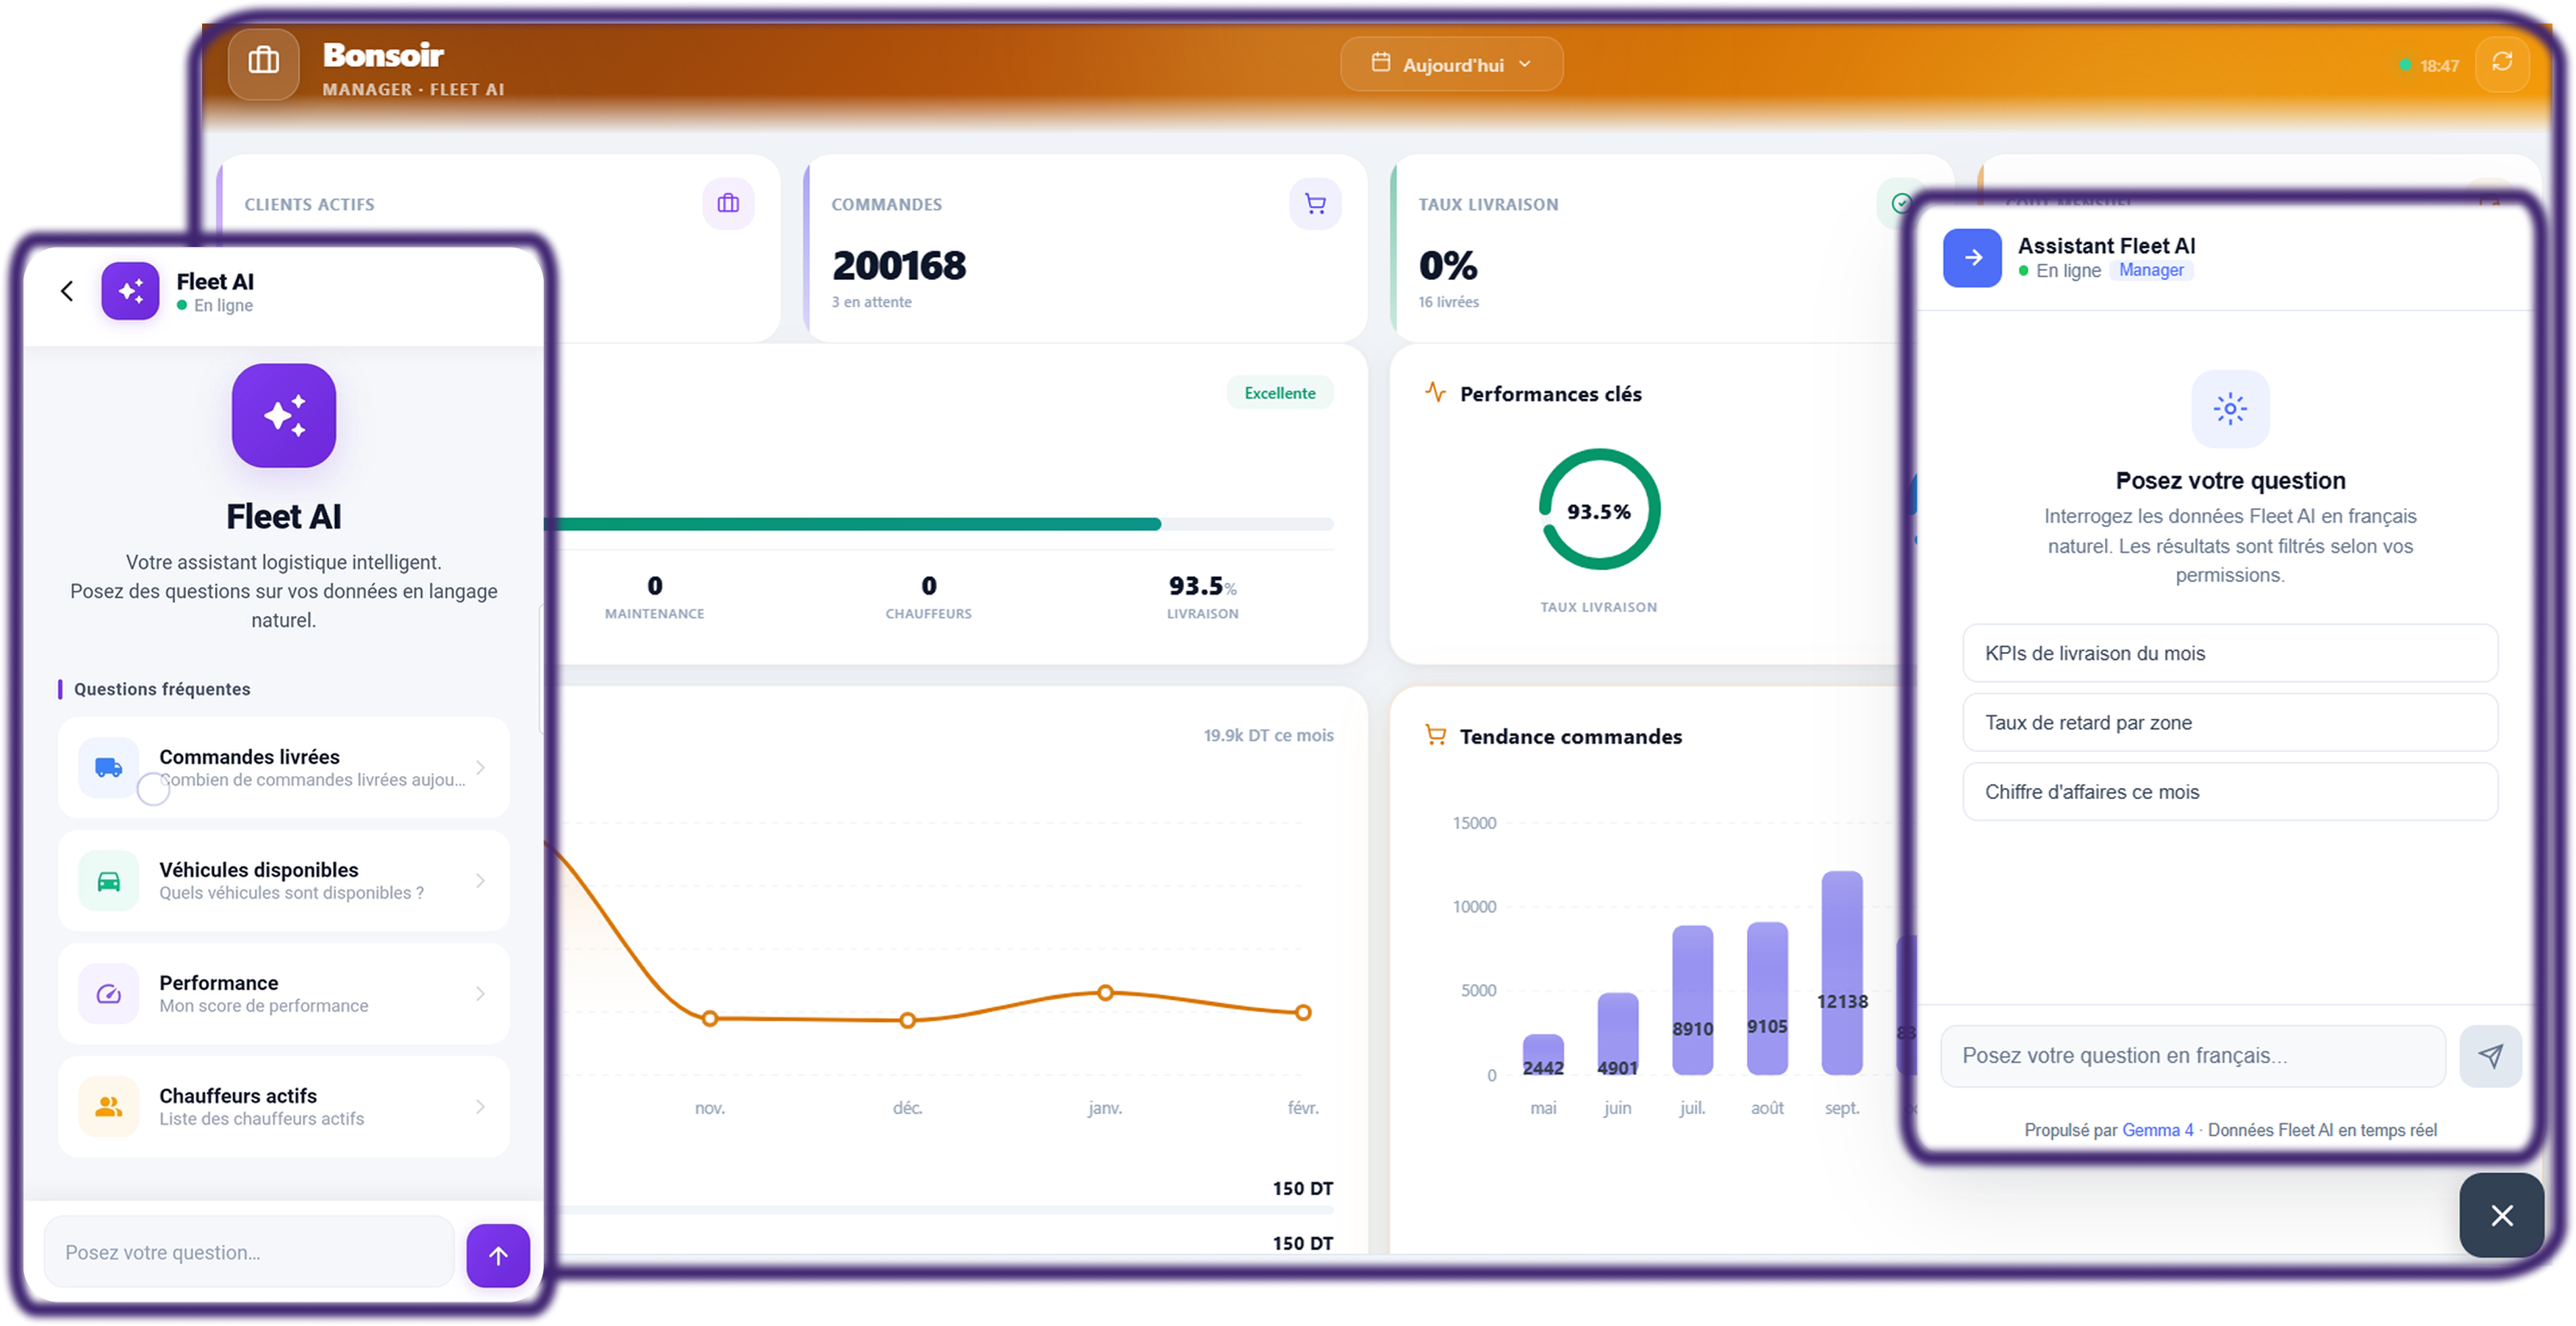
\includegraphics[width=\linewidth, keepaspectratio]{img/capture/ai/sp5_chatbot_composite}%
}{%
  \fbox{\parbox{0.9\linewidth}{\centering\vspace{4cm}\textit{[\`{}img/sp5\_chatbot\_composite\`{} --- Capture à réaliser]}\vspace{4cm}}}%
}
\caption{Intégration Chatbot Text-to-SQL : interface conversationnelle en langage naturel, génération SQL automatique et réponse reformulée par Gemma~4 31B}
\label{fig:sp5-chatbot-integration}
\end{figure}



% =============================================================
\section{Tests}
% =============================================================

Afin de valider la robustesse de la couche IA déployée, des tests de charge ont été exécutés sur l'API d'Intelligence Artificielle à l'aide de \textbf{JMeter}, simulant des appels simultanés aux six modèles ML et au chatbot Text-to-SQL.

\begin{figure}[H]
\centering
\IfFileExists{img/capture/ai/sp5_test_jmeter.png}{%
  \includegraphics[width=\linewidth, keepaspectratio]{img/capture/ai/sp5_test_jmeter}%
}{%
  \fbox{\parbox{0.9\linewidth}{\centering\vspace{4cm}\textit{[img/capture/ai/sp5\_test\_jmeter.png]}\vspace{4cm}}}%
}
\caption{Exécution d'un test de charge avec JMeter sur l'API d'Intelligence Artificielle}
\label{fig:sp5-test-jmeter}
\end{figure}

\section*{Conclusion}
\addcontentsline{toc}{section}{Conclusion}

Le Sprint~5 achève Fleet~AI. Les six modèles ML (scoring chauffeur, prévision de la demande, détection des retards, dimensionnement de flotte, apprentissage des routes, risque paiement) sont déployés via FastAPI selon la méthodologie CRISP-DM. Le chatbot Text-to-SQL fondé sur Gemma~4 31B permet d'interroger la base de données en langage naturel.


% ---- Conclusion générale ----
\newpage
\vspace*{0.6\baselineskip}
\begin{center}
  {\Huge\bfseries Conclusion générale}
\end{center}
\addcontentsline{toc}{chapter}{Conclusion générale}
\markboth{Conclusion générale}{}
\vspace{1.5cm}

Ce projet de fin d'études, réalisé chez \textbf{GREPSYS Tunisia} pour \textbf{Poulina Group Holding}, nous a conduits à concevoir et développer \textbf{Fleet~AI} de zéro : 133 user stories réparties sur cinq sprints de deux semaines, intégrées à la plateforme WFMS sans en modifier le code source.\\

Le point de départ était simple : PGH planifiait ses livraisons à la main, communiquait par téléphone et ne disposait d'aucune traçabilité des paiements. Le système livré couvre l'ensemble du cycle logistique.

Le \textbf{Sprint~1} a posé les fondations : authentification WFMS, gestion des utilisateurs avec RBAC, référentiels véhicules, chauffeurs et zones, journal d'audit et l'application mobile chauffeur. Le \textbf{Sprint~2} a introduit la gestion des clients, le workflow de commande à dix statuts et l'application mobile client. Le \textbf{Sprint~3} a ajouté la planification assistée par OR-Tools, le suivi GPS temps réel via WebSocket et la gestion enterprise des disponibilités. Le \textbf{Sprint~4} a couvert l'exécution terrain et le suivi client : preuves numériques de livraison, trois modes de paiement avec validation REC, gestion des réclamations avec escalade, notifications multicanal et mode hors ligne mobile. Le \textbf{Sprint~5} a doté la plateforme de son intelligence artificielle : modèles de prédiction ML déployés via FastAPI (scoring, demande, retards, dimensionnement, routes, risque de paiement) et un assistant conversationnel (chatbot) Text-to-SQL sécurisé.\\

Sur le plan technique, nous avons travaillé avec une pile variée (Angular 19, Spring Boot 3.4, Flutter, FastAPI, PostgreSQL, MongoDB, Redis) dans un écosystème déjà en production, ce qui impose des contraintes que les projets académiques standards n'ont pas. L'intégration avec l'ERP de PGH via un adaptateur ETL, sans toucher aux systèmes existants, a été la contrainte la plus complexe à gérer.\\

Ce stage nous a appris autant sur la gestion des contraintes d'intégration que sur les technologies elles-mêmes.



% ---- Bibliographie / Médiagraphie ----
\clearpage
\phantomsection
\addcontentsline{toc}{chapter}{Médiagraphie}
\printbibliography[title={Médiagraphie}]

\end{document}
